% Options for packages loaded elsewhere
\PassOptionsToPackage{unicode}{hyperref}
\PassOptionsToPackage{hyphens}{url}
%
\documentclass[
]{book}
\usepackage{amsmath,amssymb}
\usepackage{lmodern}
\usepackage{iftex}
\ifPDFTeX
  \usepackage[T1]{fontenc}
  \usepackage[utf8]{inputenc}
  \usepackage{textcomp} % provide euro and other symbols
\else % if luatex or xetex
  \usepackage{unicode-math}
  \defaultfontfeatures{Scale=MatchLowercase}
  \defaultfontfeatures[\rmfamily]{Ligatures=TeX,Scale=1}
\fi
% Use upquote if available, for straight quotes in verbatim environments
\IfFileExists{upquote.sty}{\usepackage{upquote}}{}
\IfFileExists{microtype.sty}{% use microtype if available
  \usepackage[]{microtype}
  \UseMicrotypeSet[protrusion]{basicmath} % disable protrusion for tt fonts
}{}
\makeatletter
\@ifundefined{KOMAClassName}{% if non-KOMA class
  \IfFileExists{parskip.sty}{%
    \usepackage{parskip}
  }{% else
    \setlength{\parindent}{0pt}
    \setlength{\parskip}{6pt plus 2pt minus 1pt}}
}{% if KOMA class
  \KOMAoptions{parskip=half}}
\makeatother
\usepackage{xcolor}
\usepackage{color}
\usepackage{fancyvrb}
\newcommand{\VerbBar}{|}
\newcommand{\VERB}{\Verb[commandchars=\\\{\}]}
\DefineVerbatimEnvironment{Highlighting}{Verbatim}{commandchars=\\\{\}}
% Add ',fontsize=\small' for more characters per line
\usepackage{framed}
\definecolor{shadecolor}{RGB}{248,248,248}
\newenvironment{Shaded}{\begin{snugshade}}{\end{snugshade}}
\newcommand{\AlertTok}[1]{\textcolor[rgb]{0.94,0.16,0.16}{#1}}
\newcommand{\AnnotationTok}[1]{\textcolor[rgb]{0.56,0.35,0.01}{\textbf{\textit{#1}}}}
\newcommand{\AttributeTok}[1]{\textcolor[rgb]{0.77,0.63,0.00}{#1}}
\newcommand{\BaseNTok}[1]{\textcolor[rgb]{0.00,0.00,0.81}{#1}}
\newcommand{\BuiltInTok}[1]{#1}
\newcommand{\CharTok}[1]{\textcolor[rgb]{0.31,0.60,0.02}{#1}}
\newcommand{\CommentTok}[1]{\textcolor[rgb]{0.56,0.35,0.01}{\textit{#1}}}
\newcommand{\CommentVarTok}[1]{\textcolor[rgb]{0.56,0.35,0.01}{\textbf{\textit{#1}}}}
\newcommand{\ConstantTok}[1]{\textcolor[rgb]{0.00,0.00,0.00}{#1}}
\newcommand{\ControlFlowTok}[1]{\textcolor[rgb]{0.13,0.29,0.53}{\textbf{#1}}}
\newcommand{\DataTypeTok}[1]{\textcolor[rgb]{0.13,0.29,0.53}{#1}}
\newcommand{\DecValTok}[1]{\textcolor[rgb]{0.00,0.00,0.81}{#1}}
\newcommand{\DocumentationTok}[1]{\textcolor[rgb]{0.56,0.35,0.01}{\textbf{\textit{#1}}}}
\newcommand{\ErrorTok}[1]{\textcolor[rgb]{0.64,0.00,0.00}{\textbf{#1}}}
\newcommand{\ExtensionTok}[1]{#1}
\newcommand{\FloatTok}[1]{\textcolor[rgb]{0.00,0.00,0.81}{#1}}
\newcommand{\FunctionTok}[1]{\textcolor[rgb]{0.00,0.00,0.00}{#1}}
\newcommand{\ImportTok}[1]{#1}
\newcommand{\InformationTok}[1]{\textcolor[rgb]{0.56,0.35,0.01}{\textbf{\textit{#1}}}}
\newcommand{\KeywordTok}[1]{\textcolor[rgb]{0.13,0.29,0.53}{\textbf{#1}}}
\newcommand{\NormalTok}[1]{#1}
\newcommand{\OperatorTok}[1]{\textcolor[rgb]{0.81,0.36,0.00}{\textbf{#1}}}
\newcommand{\OtherTok}[1]{\textcolor[rgb]{0.56,0.35,0.01}{#1}}
\newcommand{\PreprocessorTok}[1]{\textcolor[rgb]{0.56,0.35,0.01}{\textit{#1}}}
\newcommand{\RegionMarkerTok}[1]{#1}
\newcommand{\SpecialCharTok}[1]{\textcolor[rgb]{0.00,0.00,0.00}{#1}}
\newcommand{\SpecialStringTok}[1]{\textcolor[rgb]{0.31,0.60,0.02}{#1}}
\newcommand{\StringTok}[1]{\textcolor[rgb]{0.31,0.60,0.02}{#1}}
\newcommand{\VariableTok}[1]{\textcolor[rgb]{0.00,0.00,0.00}{#1}}
\newcommand{\VerbatimStringTok}[1]{\textcolor[rgb]{0.31,0.60,0.02}{#1}}
\newcommand{\WarningTok}[1]{\textcolor[rgb]{0.56,0.35,0.01}{\textbf{\textit{#1}}}}
\usepackage{longtable,booktabs,array}
\usepackage{calc} % for calculating minipage widths
% Correct order of tables after \paragraph or \subparagraph
\usepackage{etoolbox}
\makeatletter
\patchcmd\longtable{\par}{\if@noskipsec\mbox{}\fi\par}{}{}
\makeatother
% Allow footnotes in longtable head/foot
\IfFileExists{footnotehyper.sty}{\usepackage{footnotehyper}}{\usepackage{footnote}}
\makesavenoteenv{longtable}
\usepackage{graphicx}
\makeatletter
\def\maxwidth{\ifdim\Gin@nat@width>\linewidth\linewidth\else\Gin@nat@width\fi}
\def\maxheight{\ifdim\Gin@nat@height>\textheight\textheight\else\Gin@nat@height\fi}
\makeatother
% Scale images if necessary, so that they will not overflow the page
% margins by default, and it is still possible to overwrite the defaults
% using explicit options in \includegraphics[width, height, ...]{}
\setkeys{Gin}{width=\maxwidth,height=\maxheight,keepaspectratio}
% Set default figure placement to htbp
\makeatletter
\def\fps@figure{htbp}
\makeatother
\setlength{\emergencystretch}{3em} % prevent overfull lines
\providecommand{\tightlist}{%
  \setlength{\itemsep}{0pt}\setlength{\parskip}{0pt}}
\setcounter{secnumdepth}{5}
\ifLuaTeX
  \usepackage{selnolig}  % disable illegal ligatures
\fi
\IfFileExists{bookmark.sty}{\usepackage{bookmark}}{\usepackage{hyperref}}
\IfFileExists{xurl.sty}{\usepackage{xurl}}{} % add URL line breaks if available
\urlstyle{same} % disable monospaced font for URLs
\hypersetup{
  pdftitle={Everyday-R: Practical R for Data Science},
  pdfauthor={by Brian Jungmin Park},
  hidelinks,
  pdfcreator={LaTeX via pandoc}}

\title{Everyday-R: Practical R for Data Science}
\author{by Brian Jungmin Park}
\date{}

\begin{document}
\maketitle

{
\setcounter{tocdepth}{1}
\tableofcontents
}
\hypertarget{introduction}{%
\chapter{Introduction}\label{introduction}}

This book serves as a collection of R Markdown files that aims to assist users in learning the practical syntax and usage of R. Mainly, code snippets and workflow aimed at tackling everyday tasks in data science will be covered, including data cleaning, data wrangling, iterations, machine learning with \texttt{caret}, data visualization, and web app design using \texttt{Shiny}. Each broad topic will be split into chapters, though there will be some overlap.

\hypertarget{r-syntax-in-this-book}{%
\section{R syntax in this book}\label{r-syntax-in-this-book}}

Code chunks will be presented in a typical Markdown format as such, with the code output below:

\begin{Shaded}
\begin{Highlighting}[]
\FunctionTok{runif}\NormalTok{(}\AttributeTok{n =} \DecValTok{20}\NormalTok{, }\AttributeTok{min =} \DecValTok{0}\NormalTok{, }\AttributeTok{max =} \DecValTok{100}\NormalTok{)}
\end{Highlighting}
\end{Shaded}

\begin{verbatim}
##  [1] 35.324141  1.300332  3.815085 65.052808 25.930353
##  [6] 71.680373 11.756955 15.622318 92.419946 16.882423
## [11] 61.781247  7.588279 59.476065 51.196286 26.978792
## [16] 29.432249 25.140491 90.854434 87.523651 85.770563
\end{verbatim}

When using commands outside of base R, the loading of the parent package will be explicitly shown to avoid confusion:

\begin{Shaded}
\begin{Highlighting}[]
\FunctionTok{library}\NormalTok{(microbenchmark)}
\NormalTok{microbenchmark}\SpecialCharTok{::}\FunctionTok{microbenchmark}\NormalTok{(}\FunctionTok{runif}\NormalTok{(}\AttributeTok{n =} \DecValTok{20}\NormalTok{, }\AttributeTok{min =} \DecValTok{0}\NormalTok{, }\AttributeTok{max =} \DecValTok{100}\NormalTok{))}
\end{Highlighting}
\end{Shaded}

\begin{verbatim}
## Unit: microseconds
##                               expr   min    lq    mean
##  runif(n = 20, min = 0, max = 100) 1.292 1.334 1.56276
##  median    uq   max neval
##   1.459 1.584 8.043   100
\end{verbatim}

Typically in longer chains of code, I will use \texttt{\%\textgreater{}\%} from \texttt{magrittr} as a pipe. This is usually standard practice in code using packages from the \texttt{tidyverse} so it's a good habit to start using it.

Finally, here is the R version I am currently using:

\begin{Shaded}
\begin{Highlighting}[]
\NormalTok{version}
\end{Highlighting}
\end{Shaded}

\begin{verbatim}
##                _                           
## platform       x86_64-apple-darwin17.0     
## arch           x86_64                      
## os             darwin17.0                  
## system         x86_64, darwin17.0          
## status                                     
## major          4                           
## minor          0.5                         
## year           2021                        
## month          03                          
## day            31                          
## svn rev        80133                       
## language       R                           
## version.string R version 4.0.5 (2021-03-31)
## nickname       Shake and Throw
\end{verbatim}

\hypertarget{r-packages-commonly-used-in-this-book}{%
\section{R packages commonly used in this book}\label{r-packages-commonly-used-in-this-book}}

\begin{itemize}
\item
  \texttt{tidyverse}: a collection of packages for data science, including \texttt{dplyr}, \texttt{purrr}, \texttt{stringr}, \texttt{forcats}, \texttt{readr}, and \texttt{ggplot}.
\item
  \texttt{caret}: package for implementation of machine learning models, with support for algorithms such as \texttt{ranger}, \texttt{rpart}, \texttt{xgbTree}, and \texttt{svmLinear}.
\item
  \texttt{mlbench}: package for benchmarks and datasets in machine learning.
\item
  \texttt{broom}: package for summarizing of model estimates.
\item
  \texttt{ggpubr}: package for publication-ready data visualizations.
\item
  \texttt{Shiny}: package for implementation and designing of interactive web apps.
\end{itemize}

\hypertarget{installing-r-packages}{%
\section{Installing R packages}\label{installing-r-packages}}

R packages found in this book are available on CRAN and thus can be installed simply by running \texttt{install.packages()}. For packages not on CRAN (or if you want to download developmental versions of a package), you can install packages straight from a GitHub repository by running \texttt{devtools::install\_github()}.

\hypertarget{code-availability}{%
\section{Code availability}\label{code-availability}}

All code used to compile this book as well as the individual markdown files are available on my repository \href{https://github.com/snowoflondon/everyday-r}{here}

\hypertarget{website-hosting}{%
\section{Website hosting}\label{website-hosting}}

This book is hosted on the \texttt{shinyapps} server, deployed with the R package \texttt{rsconnect}. The markdown files are compiled in this book format using the R package \texttt{bookdown}.

\hypertarget{everyday-data-wrangling}{%
\chapter{Everyday data wrangling}\label{everyday-data-wrangling}}

Suppose there exists a test dataset and the user is tasked with proving their proficiency in exploratory data analysis (EDA). Alternatively, the user may be handed a piece of data (e.g., maybe an Excel sheet) and is asked to run some preliminary analysis. Prior to jumping straight into EDA and statistical modeling, the user must be able to transform the original data into a desirable format. This includes, but is not limited to, missing data imputation, scalar transformation, feature selection, group aggregation, and data filtering. The following notebook outlines the fundamentals of data wrangling, using practical base R and \texttt{tidyverse} solutions interchangeably.

\begin{Shaded}
\begin{Highlighting}[]
\FunctionTok{library}\NormalTok{(tidyverse)}
\end{Highlighting}
\end{Shaded}

\begin{verbatim}
## -- Attaching packages -------------------- tidyverse 1.3.1 --
\end{verbatim}

\begin{verbatim}
## v ggplot2 3.4.1     v purrr   1.0.1
## v tibble  3.2.0     v dplyr   1.1.0
## v tidyr   1.3.0     v stringr 1.5.0
## v readr   1.4.0     v forcats 0.5.1
\end{verbatim}

\begin{verbatim}
## -- Conflicts ----------------------- tidyverse_conflicts() --
## x dplyr::filter() masks stats::filter()
## x dplyr::lag()    masks stats::lag()
\end{verbatim}

\hypertarget{renaming-column-headers}{%
\section{Renaming column headers}\label{renaming-column-headers}}

Suppose a \texttt{32\ x\ 11} dataset \texttt{mtcars} where \texttt{rownames} correspond to the car model.

\begin{Shaded}
\begin{Highlighting}[]
\FunctionTok{data}\NormalTok{(mtcars)}
\NormalTok{mtcars }\OtherTok{\textless{}{-}}\NormalTok{ mtcars }\SpecialCharTok{\%\textgreater{}\%} \FunctionTok{as\_tibble}\NormalTok{(}\AttributeTok{rownames =} \StringTok{\textquotesingle{}CAR\textquotesingle{}}\NormalTok{)}
\end{Highlighting}
\end{Shaded}

Renaming column headers with \texttt{dplyr::rename} is as simple as \texttt{rename(new\_name\ =\ old\_name)}, but with \texttt{rename\_with()} there's more flexibility:

\begin{Shaded}
\begin{Highlighting}[]
\NormalTok{mtcars }\SpecialCharTok{\%\textgreater{}\%} \FunctionTok{rename\_with}\NormalTok{(toupper)}
\end{Highlighting}
\end{Shaded}

\begin{verbatim}
## # A tibble: 32 x 12
##    CAR          MPG   CYL  DISP    HP  DRAT    WT  QSEC    VS
##    <chr>      <dbl> <dbl> <dbl> <dbl> <dbl> <dbl> <dbl> <dbl>
##  1 Mazda RX4   21       6  160    110  3.9   2.62  16.5     0
##  2 Mazda RX4~  21       6  160    110  3.9   2.88  17.0     0
##  3 Datsun 710  22.8     4  108     93  3.85  2.32  18.6     1
##  4 Hornet 4 ~  21.4     6  258    110  3.08  3.22  19.4     1
##  5 Hornet Sp~  18.7     8  360    175  3.15  3.44  17.0     0
##  6 Valiant     18.1     6  225    105  2.76  3.46  20.2     1
##  7 Duster 360  14.3     8  360    245  3.21  3.57  15.8     0
##  8 Merc 240D   24.4     4  147.    62  3.69  3.19  20       1
##  9 Merc 230    22.8     4  141.    95  3.92  3.15  22.9     1
## 10 Merc 280    19.2     6  168.   123  3.92  3.44  18.3     1
## # ... with 22 more rows, and 3 more variables: AM <dbl>,
## #   GEAR <dbl>, CARB <dbl>
\end{verbatim}

You can pass any function within \texttt{rename\_with()} to alter the column headers and use the \texttt{.cols\ =} argument to define which columns you'd apply the function to:

\begin{Shaded}
\begin{Highlighting}[]
\NormalTok{mtcars }\SpecialCharTok{\%\textgreater{}\%} \FunctionTok{rename\_with}\NormalTok{(}\ControlFlowTok{function}\NormalTok{(x) }\FunctionTok{paste0}\NormalTok{(x, }\StringTok{"\_1"}\NormalTok{), }\AttributeTok{.cols =} \SpecialCharTok{{-}}\DecValTok{1}\NormalTok{)}
\end{Highlighting}
\end{Shaded}

\begin{verbatim}
## # A tibble: 32 x 12
##    CAR     mpg_1 cyl_1 disp_1  hp_1 drat_1  wt_1 qsec_1  vs_1
##    <chr>   <dbl> <dbl>  <dbl> <dbl>  <dbl> <dbl>  <dbl> <dbl>
##  1 Mazda ~  21       6   160    110   3.9   2.62   16.5     0
##  2 Mazda ~  21       6   160    110   3.9   2.88   17.0     0
##  3 Datsun~  22.8     4   108     93   3.85  2.32   18.6     1
##  4 Hornet~  21.4     6   258    110   3.08  3.22   19.4     1
##  5 Hornet~  18.7     8   360    175   3.15  3.44   17.0     0
##  6 Valiant  18.1     6   225    105   2.76  3.46   20.2     1
##  7 Duster~  14.3     8   360    245   3.21  3.57   15.8     0
##  8 Merc 2~  24.4     4   147.    62   3.69  3.19   20       1
##  9 Merc 2~  22.8     4   141.    95   3.92  3.15   22.9     1
## 10 Merc 2~  19.2     6   168.   123   3.92  3.44   18.3     1
## # ... with 22 more rows, and 3 more variables: am_1 <dbl>,
## #   gear_1 <dbl>, carb_1 <dbl>
\end{verbatim}

Alternatively with base R, you can call the \texttt{names} attribute and alter that directly:

\begin{Shaded}
\begin{Highlighting}[]
\FunctionTok{names}\NormalTok{(mtcars)[}\SpecialCharTok{{-}}\DecValTok{1}\NormalTok{] }\OtherTok{\textless{}{-}} \FunctionTok{paste0}\NormalTok{(}\FunctionTok{names}\NormalTok{(mtcars[}\SpecialCharTok{{-}}\DecValTok{1}\NormalTok{]), }\StringTok{\textquotesingle{}\_1\textquotesingle{}}\NormalTok{) }\CommentTok{\# not run}
\end{Highlighting}
\end{Shaded}

\hypertarget{grouped-operations}{%
\section{Grouped operations}\label{grouped-operations}}

Grouped operations are most useful when you're working with data where there is a categorical variable. Grouped summaries are powerful tools easily done with \texttt{dplyr::summarise}:

\begin{Shaded}
\begin{Highlighting}[]
\NormalTok{mtcars }\SpecialCharTok{\%\textgreater{}\%} \FunctionTok{group\_by}\NormalTok{(cyl) }\SpecialCharTok{\%\textgreater{}\%} \FunctionTok{summarise}\NormalTok{(}\AttributeTok{avg\_mpg =} \FunctionTok{mean}\NormalTok{(mpg))}
\end{Highlighting}
\end{Shaded}

\begin{verbatim}
## # A tibble: 3 x 2
##     cyl avg_mpg
##   <dbl>   <dbl>
## 1     4    26.7
## 2     6    19.7
## 3     8    15.1
\end{verbatim}

Using multiple columns at once and renaming the output columns:

\begin{Shaded}
\begin{Highlighting}[]
\NormalTok{mtcars }\SpecialCharTok{\%\textgreater{}\%} \FunctionTok{group\_by}\NormalTok{(cyl) }\SpecialCharTok{\%\textgreater{}\%} 
  \FunctionTok{summarise}\NormalTok{(}\FunctionTok{across}\NormalTok{(}\FunctionTok{c}\NormalTok{(mpg, disp, hp), mean, }\AttributeTok{.names =} \StringTok{"mean\_\{col\}"}\NormalTok{))}
\end{Highlighting}
\end{Shaded}

\begin{verbatim}
## # A tibble: 3 x 4
##     cyl mean_mpg mean_disp mean_hp
##   <dbl>    <dbl>     <dbl>   <dbl>
## 1     4     26.7      105.    82.6
## 2     6     19.7      183.   122. 
## 3     8     15.1      353.   209.
\end{verbatim}

\begin{Shaded}
\begin{Highlighting}[]
\NormalTok{mtcars }\SpecialCharTok{\%\textgreater{}\%} \FunctionTok{group\_by}\NormalTok{(cyl) }\SpecialCharTok{\%\textgreater{}\%} 
  \FunctionTok{summarise}\NormalTok{(}\FunctionTok{across}\NormalTok{(}\FunctionTok{where}\NormalTok{(is.numeric), mean, }\AttributeTok{.names =} \StringTok{"mean\_\{col\}"}\NormalTok{))}
\end{Highlighting}
\end{Shaded}

\begin{verbatim}
## # A tibble: 3 x 11
##     cyl mean_mpg mean_disp mean_hp mean_drat mean_wt mean_q~1
##   <dbl>    <dbl>     <dbl>   <dbl>     <dbl>   <dbl>    <dbl>
## 1     4     26.7      105.    82.6      4.07    2.29     19.1
## 2     6     19.7      183.   122.       3.59    3.12     18.0
## 3     8     15.1      353.   209.       3.23    4.00     16.8
## # ... with 4 more variables: mean_vs <dbl>, mean_am <dbl>,
## #   mean_gear <dbl>, mean_carb <dbl>, and abbreviated
## #   variable name 1: mean_qsec
\end{verbatim}

Alternatively, in base R, you can use \texttt{aggregate()} with the \texttt{\textasciitilde{}}; you can read this as \emph{grouping mpg by cyl} where \emph{by} corresponds to the \texttt{\textasciitilde{}}:

\begin{Shaded}
\begin{Highlighting}[]
\FunctionTok{aggregate}\NormalTok{(mpg }\SpecialCharTok{\textasciitilde{}}\NormalTok{ cyl, }\AttributeTok{data =}\NormalTok{ mtcars, }\AttributeTok{FUN =}\NormalTok{ mean)}
\end{Highlighting}
\end{Shaded}

\begin{verbatim}
##   cyl      mpg
## 1   4 26.66364
## 2   6 19.74286
## 3   8 15.10000
\end{verbatim}

When calculating the size of the groups, you can use \texttt{n()}:

\begin{Shaded}
\begin{Highlighting}[]
\NormalTok{mtcars }\SpecialCharTok{\%\textgreater{}\%} \FunctionTok{group\_by}\NormalTok{(cyl) }\SpecialCharTok{\%\textgreater{}\%} \FunctionTok{summarise}\NormalTok{(}\AttributeTok{count =} \FunctionTok{n}\NormalTok{())}
\end{Highlighting}
\end{Shaded}

\begin{verbatim}
## # A tibble: 3 x 2
##     cyl count
##   <dbl> <int>
## 1     4    11
## 2     6     7
## 3     8    14
\end{verbatim}

Filtering by groups of size greater than a certain value:

\begin{Shaded}
\begin{Highlighting}[]
\NormalTok{mtcars }\SpecialCharTok{\%\textgreater{}\%} \FunctionTok{group\_by}\NormalTok{(cyl) }\SpecialCharTok{\%\textgreater{}\%} \FunctionTok{filter}\NormalTok{(}\FunctionTok{n}\NormalTok{() }\SpecialCharTok{\textgreater{}} \DecValTok{7}\NormalTok{) }\SpecialCharTok{\%\textgreater{}\%} \FunctionTok{ungroup}\NormalTok{()}
\end{Highlighting}
\end{Shaded}

\begin{verbatim}
## # A tibble: 25 x 12
##    CAR          mpg   cyl  disp    hp  drat    wt  qsec    vs
##    <chr>      <dbl> <dbl> <dbl> <dbl> <dbl> <dbl> <dbl> <dbl>
##  1 Datsun 710  22.8     4  108     93  3.85  2.32  18.6     1
##  2 Hornet Sp~  18.7     8  360    175  3.15  3.44  17.0     0
##  3 Duster 360  14.3     8  360    245  3.21  3.57  15.8     0
##  4 Merc 240D   24.4     4  147.    62  3.69  3.19  20       1
##  5 Merc 230    22.8     4  141.    95  3.92  3.15  22.9     1
##  6 Merc 450SE  16.4     8  276.   180  3.07  4.07  17.4     0
##  7 Merc 450SL  17.3     8  276.   180  3.07  3.73  17.6     0
##  8 Merc 450S~  15.2     8  276.   180  3.07  3.78  18       0
##  9 Cadillac ~  10.4     8  472    205  2.93  5.25  18.0     0
## 10 Lincoln C~  10.4     8  460    215  3     5.42  17.8     0
## # ... with 15 more rows, and 3 more variables: am <dbl>,
## #   gear <dbl>, carb <dbl>
\end{verbatim}

\hypertarget{data-transformation}{%
\section{Data transformation}\label{data-transformation}}

Sometimes it's useful to transform numeric columns:

\begin{Shaded}
\begin{Highlighting}[]
\NormalTok{mtcars }\SpecialCharTok{\%\textgreater{}\%} \FunctionTok{mutate}\NormalTok{(}\AttributeTok{mpg =}\NormalTok{ mpg}\SpecialCharTok{*}\DecValTok{2}\NormalTok{)}
\end{Highlighting}
\end{Shaded}

\begin{verbatim}
## # A tibble: 32 x 12
##    CAR          mpg   cyl  disp    hp  drat    wt  qsec    vs
##    <chr>      <dbl> <dbl> <dbl> <dbl> <dbl> <dbl> <dbl> <dbl>
##  1 Mazda RX4   42       6  160    110  3.9   2.62  16.5     0
##  2 Mazda RX4~  42       6  160    110  3.9   2.88  17.0     0
##  3 Datsun 710  45.6     4  108     93  3.85  2.32  18.6     1
##  4 Hornet 4 ~  42.8     6  258    110  3.08  3.22  19.4     1
##  5 Hornet Sp~  37.4     8  360    175  3.15  3.44  17.0     0
##  6 Valiant     36.2     6  225    105  2.76  3.46  20.2     1
##  7 Duster 360  28.6     8  360    245  3.21  3.57  15.8     0
##  8 Merc 240D   48.8     4  147.    62  3.69  3.19  20       1
##  9 Merc 230    45.6     4  141.    95  3.92  3.15  22.9     1
## 10 Merc 280    38.4     6  168.   123  3.92  3.44  18.3     1
## # ... with 22 more rows, and 3 more variables: am <dbl>,
## #   gear <dbl>, carb <dbl>
\end{verbatim}

Using \texttt{across()} allows for conditional transformation and keep the old columns, while renaming the new columns:

\begin{Shaded}
\begin{Highlighting}[]
\NormalTok{mtcars }\SpecialCharTok{\%\textgreater{}\%} 
  \FunctionTok{mutate}\NormalTok{(}\FunctionTok{across}\NormalTok{(}\FunctionTok{where}\NormalTok{(is.numeric), }\ControlFlowTok{function}\NormalTok{(x) x}\SpecialCharTok{*}\DecValTok{2}\NormalTok{, }\AttributeTok{.names =} \StringTok{"double\_\{col\}"}\NormalTok{))}
\end{Highlighting}
\end{Shaded}

\begin{verbatim}
## # A tibble: 32 x 23
##    CAR          mpg   cyl  disp    hp  drat    wt  qsec    vs
##    <chr>      <dbl> <dbl> <dbl> <dbl> <dbl> <dbl> <dbl> <dbl>
##  1 Mazda RX4   21       6  160    110  3.9   2.62  16.5     0
##  2 Mazda RX4~  21       6  160    110  3.9   2.88  17.0     0
##  3 Datsun 710  22.8     4  108     93  3.85  2.32  18.6     1
##  4 Hornet 4 ~  21.4     6  258    110  3.08  3.22  19.4     1
##  5 Hornet Sp~  18.7     8  360    175  3.15  3.44  17.0     0
##  6 Valiant     18.1     6  225    105  2.76  3.46  20.2     1
##  7 Duster 360  14.3     8  360    245  3.21  3.57  15.8     0
##  8 Merc 240D   24.4     4  147.    62  3.69  3.19  20       1
##  9 Merc 230    22.8     4  141.    95  3.92  3.15  22.9     1
## 10 Merc 280    19.2     6  168.   123  3.92  3.44  18.3     1
## # ... with 22 more rows, and 14 more variables: am <dbl>,
## #   gear <dbl>, carb <dbl>, double_mpg <dbl>,
## #   double_cyl <dbl>, double_disp <dbl>, double_hp <dbl>,
## #   double_drat <dbl>, double_wt <dbl>, double_qsec <dbl>,
## #   double_vs <dbl>, double_am <dbl>, double_gear <dbl>,
## #   double_carb <dbl>
\end{verbatim}

You can overwrite the existing columns completely; also keep in mind that you can pass any function within \texttt{across()} as such:

\begin{Shaded}
\begin{Highlighting}[]
\NormalTok{mtcars }\SpecialCharTok{\%\textgreater{}\%} \FunctionTok{mutate}\NormalTok{(}\FunctionTok{across}\NormalTok{(}\FunctionTok{c}\NormalTok{(mpg, disp), }\ControlFlowTok{function}\NormalTok{(x) x}\SpecialCharTok{*}\DecValTok{3}\NormalTok{))}
\end{Highlighting}
\end{Shaded}

\begin{verbatim}
## # A tibble: 32 x 12
##    CAR          mpg   cyl  disp    hp  drat    wt  qsec    vs
##    <chr>      <dbl> <dbl> <dbl> <dbl> <dbl> <dbl> <dbl> <dbl>
##  1 Mazda RX4   63       6  480    110  3.9   2.62  16.5     0
##  2 Mazda RX4~  63       6  480    110  3.9   2.88  17.0     0
##  3 Datsun 710  68.4     4  324     93  3.85  2.32  18.6     1
##  4 Hornet 4 ~  64.2     6  774    110  3.08  3.22  19.4     1
##  5 Hornet Sp~  56.1     8 1080    175  3.15  3.44  17.0     0
##  6 Valiant     54.3     6  675    105  2.76  3.46  20.2     1
##  7 Duster 360  42.9     8 1080    245  3.21  3.57  15.8     0
##  8 Merc 240D   73.2     4  440.    62  3.69  3.19  20       1
##  9 Merc 230    68.4     4  422.    95  3.92  3.15  22.9     1
## 10 Merc 280    57.6     6  503.   123  3.92  3.44  18.3     1
## # ... with 22 more rows, and 3 more variables: am <dbl>,
## #   gear <dbl>, carb <dbl>
\end{verbatim}

Iterating across the columns using \texttt{purrr::modify} instead:

\begin{Shaded}
\begin{Highlighting}[]
\NormalTok{mtcars }\SpecialCharTok{\%\textgreater{}\%} \FunctionTok{modify\_if}\NormalTok{(is.numeric, }\SpecialCharTok{\textasciitilde{}}\NormalTok{ .x}\SpecialCharTok{*}\DecValTok{3}\NormalTok{)}
\end{Highlighting}
\end{Shaded}

\begin{verbatim}
## # A tibble: 32 x 12
##    CAR          mpg   cyl  disp    hp  drat    wt  qsec    vs
##    <chr>      <dbl> <dbl> <dbl> <dbl> <dbl> <dbl> <dbl> <dbl>
##  1 Mazda RX4   63      18  480    330 11.7   7.86  49.4     0
##  2 Mazda RX4~  63      18  480    330 11.7   8.62  51.1     0
##  3 Datsun 710  68.4    12  324    279 11.6   6.96  55.8     3
##  4 Hornet 4 ~  64.2    18  774    330  9.24  9.64  58.3     3
##  5 Hornet Sp~  56.1    24 1080    525  9.45 10.3   51.1     0
##  6 Valiant     54.3    18  675    315  8.28 10.4   60.7     3
##  7 Duster 360  42.9    24 1080    735  9.63 10.7   47.5     0
##  8 Merc 240D   73.2    12  440.   186 11.1   9.57  60       3
##  9 Merc 230    68.4    12  422.   285 11.8   9.45  68.7     3
## 10 Merc 280    57.6    18  503.   369 11.8  10.3   54.9     3
## # ... with 22 more rows, and 3 more variables: am <dbl>,
## #   gear <dbl>, carb <dbl>
\end{verbatim}

Mutating columns of characters is also straightforward:

\begin{Shaded}
\begin{Highlighting}[]
\NormalTok{mtcars }\SpecialCharTok{\%\textgreater{}\%} \FunctionTok{mutate}\NormalTok{(}\AttributeTok{CAR =} \FunctionTok{gsub}\NormalTok{(}\StringTok{\textquotesingle{}Merc\textquotesingle{}}\NormalTok{, }\StringTok{\textquotesingle{}Mercedes\textquotesingle{}}\NormalTok{, CAR))}
\end{Highlighting}
\end{Shaded}

\begin{verbatim}
## # A tibble: 32 x 12
##    CAR          mpg   cyl  disp    hp  drat    wt  qsec    vs
##    <chr>      <dbl> <dbl> <dbl> <dbl> <dbl> <dbl> <dbl> <dbl>
##  1 Mazda RX4   21       6  160    110  3.9   2.62  16.5     0
##  2 Mazda RX4~  21       6  160    110  3.9   2.88  17.0     0
##  3 Datsun 710  22.8     4  108     93  3.85  2.32  18.6     1
##  4 Hornet 4 ~  21.4     6  258    110  3.08  3.22  19.4     1
##  5 Hornet Sp~  18.7     8  360    175  3.15  3.44  17.0     0
##  6 Valiant     18.1     6  225    105  2.76  3.46  20.2     1
##  7 Duster 360  14.3     8  360    245  3.21  3.57  15.8     0
##  8 Mercedes ~  24.4     4  147.    62  3.69  3.19  20       1
##  9 Mercedes ~  22.8     4  141.    95  3.92  3.15  22.9     1
## 10 Mercedes ~  19.2     6  168.   123  3.92  3.44  18.3     1
## # ... with 22 more rows, and 3 more variables: am <dbl>,
## #   gear <dbl>, carb <dbl>
\end{verbatim}

\begin{Shaded}
\begin{Highlighting}[]
\NormalTok{mtcars }\SpecialCharTok{\%\textgreater{}\%} \FunctionTok{mutate}\NormalTok{(}\AttributeTok{CAR =} \FunctionTok{gsub}\NormalTok{(}\StringTok{\textquotesingle{} \textquotesingle{}}\NormalTok{, }\StringTok{\textquotesingle{}\_\textquotesingle{}}\NormalTok{, CAR)) }\SpecialCharTok{\%\textgreater{}\%} \FunctionTok{mutate}\NormalTok{(}\FunctionTok{across}\NormalTok{(CAR, tolower))}
\end{Highlighting}
\end{Shaded}

\begin{verbatim}
## # A tibble: 32 x 12
##    CAR          mpg   cyl  disp    hp  drat    wt  qsec    vs
##    <chr>      <dbl> <dbl> <dbl> <dbl> <dbl> <dbl> <dbl> <dbl>
##  1 mazda_rx4   21       6  160    110  3.9   2.62  16.5     0
##  2 mazda_rx4~  21       6  160    110  3.9   2.88  17.0     0
##  3 datsun_710  22.8     4  108     93  3.85  2.32  18.6     1
##  4 hornet_4_~  21.4     6  258    110  3.08  3.22  19.4     1
##  5 hornet_sp~  18.7     8  360    175  3.15  3.44  17.0     0
##  6 valiant     18.1     6  225    105  2.76  3.46  20.2     1
##  7 duster_360  14.3     8  360    245  3.21  3.57  15.8     0
##  8 merc_240d   24.4     4  147.    62  3.69  3.19  20       1
##  9 merc_230    22.8     4  141.    95  3.92  3.15  22.9     1
## 10 merc_280    19.2     6  168.   123  3.92  3.44  18.3     1
## # ... with 22 more rows, and 3 more variables: am <dbl>,
## #   gear <dbl>, carb <dbl>
\end{verbatim}

\hypertarget{joining-and-separating-character-columns}{%
\section{Joining and separating character columns}\label{joining-and-separating-character-columns}}

For the \texttt{CAR} column comprised of strings, you can separate the individual strings into multiple columns; the \texttt{extra\ =\ \textquotesingle{}merge\textquotesingle{}} argument tells the function to separate the string based on the first instance of '' '' and merge the rest:

\begin{Shaded}
\begin{Highlighting}[]
\NormalTok{mtcars }\SpecialCharTok{\%\textgreater{}\%} \FunctionTok{separate}\NormalTok{(CAR, }\FunctionTok{c}\NormalTok{(}\StringTok{\textquotesingle{}Brand\textquotesingle{}}\NormalTok{, }\StringTok{\textquotesingle{}Model\textquotesingle{}}\NormalTok{), }\AttributeTok{sep =} \StringTok{" "}\NormalTok{, }\AttributeTok{extra =} \StringTok{\textquotesingle{}merge\textquotesingle{}}\NormalTok{)}
\end{Highlighting}
\end{Shaded}

\begin{verbatim}
## # A tibble: 32 x 13
##    Brand   Model      mpg   cyl  disp    hp  drat    wt  qsec
##    <chr>   <chr>    <dbl> <dbl> <dbl> <dbl> <dbl> <dbl> <dbl>
##  1 Mazda   RX4       21       6  160    110  3.9   2.62  16.5
##  2 Mazda   RX4 Wag   21       6  160    110  3.9   2.88  17.0
##  3 Datsun  710       22.8     4  108     93  3.85  2.32  18.6
##  4 Hornet  4 Drive   21.4     6  258    110  3.08  3.22  19.4
##  5 Hornet  Sportab~  18.7     8  360    175  3.15  3.44  17.0
##  6 Valiant <NA>      18.1     6  225    105  2.76  3.46  20.2
##  7 Duster  360       14.3     8  360    245  3.21  3.57  15.8
##  8 Merc    240D      24.4     4  147.    62  3.69  3.19  20  
##  9 Merc    230       22.8     4  141.    95  3.92  3.15  22.9
## 10 Merc    280       19.2     6  168.   123  3.92  3.44  18.3
## # ... with 22 more rows, and 4 more variables: vs <dbl>,
## #   am <dbl>, gear <dbl>, carb <dbl>
\end{verbatim}

Combining multiple \texttt{tidyverse} verbs using the pipe \texttt{\%\textgreater{}\%}:

\begin{Shaded}
\begin{Highlighting}[]
\NormalTok{mtcars }\SpecialCharTok{\%\textgreater{}\%} \FunctionTok{separate}\NormalTok{(CAR, }\FunctionTok{c}\NormalTok{(}\StringTok{\textquotesingle{}Brand\textquotesingle{}}\NormalTok{, }\StringTok{\textquotesingle{}Model\textquotesingle{}}\NormalTok{), }\AttributeTok{sep =} \StringTok{" "}\NormalTok{, }\AttributeTok{extra =} \StringTok{\textquotesingle{}merge\textquotesingle{}}\NormalTok{) }\SpecialCharTok{\%\textgreater{}\%}
  \FunctionTok{group\_by}\NormalTok{(Brand) }\SpecialCharTok{\%\textgreater{}\%} \FunctionTok{summarise}\NormalTok{(}\AttributeTok{count =} \FunctionTok{n}\NormalTok{(), }\AttributeTok{mean\_mpg =} \FunctionTok{mean}\NormalTok{(mpg)) }\SpecialCharTok{\%\textgreater{}\%}
  \FunctionTok{arrange}\NormalTok{(}\FunctionTok{desc}\NormalTok{(count))}
\end{Highlighting}
\end{Shaded}

\begin{verbatim}
## # A tibble: 22 x 3
##    Brand    count mean_mpg
##    <chr>    <int>    <dbl>
##  1 Merc         7     19.0
##  2 Fiat         2     29.8
##  3 Hornet       2     20.0
##  4 Mazda        2     21  
##  5 Toyota       2     27.7
##  6 AMC          1     15.2
##  7 Cadillac     1     10.4
##  8 Camaro       1     13.3
##  9 Chrysler     1     14.7
## 10 Datsun       1     22.8
## # ... with 12 more rows
\end{verbatim}

Note that the pipe \texttt{\%\textgreater{}\%} is part of the \texttt{magrittr} package but there's no need to load it after loading \texttt{tidyverse}. The pipe notation is frequently used between \texttt{tidyverse} verbs but you can also use it in some base R operations as well.

Separation of columns by strings, using base R instead involves using \texttt{strsplit()} which outputs a list and therefore we need to unpack it afterwards:

\begin{Shaded}
\begin{Highlighting}[]
\NormalTok{mtcars}\SpecialCharTok{$}\NormalTok{Brand }\OtherTok{\textless{}{-}} \FunctionTok{unlist}\NormalTok{(}
  \FunctionTok{lapply}\NormalTok{(}\FunctionTok{strsplit}\NormalTok{(mtcars}\SpecialCharTok{$}\NormalTok{CAR, }\AttributeTok{split =} \StringTok{\textquotesingle{} \textquotesingle{}}\NormalTok{), }\ControlFlowTok{function}\NormalTok{(x) x[}\DecValTok{1}\NormalTok{])}
\NormalTok{) }\CommentTok{\# not run}
\NormalTok{mtcars}\SpecialCharTok{$}\NormalTok{Model }\OtherTok{\textless{}{-}} \FunctionTok{unlist}\NormalTok{(}
  \FunctionTok{lapply}\NormalTok{(}\FunctionTok{strsplit}\NormalTok{(mtcars}\SpecialCharTok{$}\NormalTok{CAR, }\AttributeTok{split =} \StringTok{\textquotesingle{} \textquotesingle{}}\NormalTok{), }\ControlFlowTok{function}\NormalTok{(x) x[}\DecValTok{2}\NormalTok{])}
\NormalTok{) }\CommentTok{\# not run}
\end{Highlighting}
\end{Shaded}

The opposite of \texttt{separate()} is \texttt{unite()} which combines columns into a single column:

\begin{Shaded}
\begin{Highlighting}[]
\FunctionTok{data}\NormalTok{(iris)}
\NormalTok{iris }\OtherTok{\textless{}{-}} \FunctionTok{as\_tibble}\NormalTok{(iris)}
\NormalTok{iris }\SpecialCharTok{\%\textgreater{}\%} \FunctionTok{unite}\NormalTok{(}\StringTok{\textquotesingle{}Petal.Dimensions\textquotesingle{}}\NormalTok{, }\FunctionTok{c}\NormalTok{(}\StringTok{\textasciigrave{}}\AttributeTok{Petal.Length}\StringTok{\textasciigrave{}}\NormalTok{, }\StringTok{\textasciigrave{}}\AttributeTok{Petal.Width}\StringTok{\textasciigrave{}}\NormalTok{),}
               \AttributeTok{sep =} \StringTok{" x "}\NormalTok{, }\AttributeTok{remove =} \ConstantTok{FALSE}\NormalTok{)}
\end{Highlighting}
\end{Shaded}

\begin{verbatim}
## # A tibble: 150 x 6
##    Sepal.Length Sepal.Width Petal.D~1 Petal~2 Petal~3 Species
##           <dbl>       <dbl> <chr>       <dbl>   <dbl> <fct>  
##  1          5.1         3.5 1.4 x 0.2     1.4     0.2 setosa 
##  2          4.9         3   1.4 x 0.2     1.4     0.2 setosa 
##  3          4.7         3.2 1.3 x 0.2     1.3     0.2 setosa 
##  4          4.6         3.1 1.5 x 0.2     1.5     0.2 setosa 
##  5          5           3.6 1.4 x 0.2     1.4     0.2 setosa 
##  6          5.4         3.9 1.7 x 0.4     1.7     0.4 setosa 
##  7          4.6         3.4 1.4 x 0.3     1.4     0.3 setosa 
##  8          5           3.4 1.5 x 0.2     1.5     0.2 setosa 
##  9          4.4         2.9 1.4 x 0.2     1.4     0.2 setosa 
## 10          4.9         3.1 1.5 x 0.1     1.5     0.1 setosa 
## # ... with 140 more rows, and abbreviated variable names
## #   1: Petal.Dimensions, 2: Petal.Length, 3: Petal.Width
\end{verbatim}

In base R, we create a new column using the \texttt{\$} notation:

\begin{Shaded}
\begin{Highlighting}[]
\NormalTok{iris}\SpecialCharTok{$}\NormalTok{Petal.Dimensions }\OtherTok{\textless{}{-}} \FunctionTok{paste}\NormalTok{(iris}\SpecialCharTok{$}\NormalTok{Petal.Length, iris}\SpecialCharTok{$}\NormalTok{Petal.Width, }\AttributeTok{sep =} \StringTok{" x "}\NormalTok{) }\CommentTok{\# not run}
\end{Highlighting}
\end{Shaded}

\hypertarget{filtering-rows}{%
\section{Filtering rows}\label{filtering-rows}}

Typically, filtering involves a condition based on a column to select the corresponding rows. Here I am combining \texttt{stringr::str\_detect} with \texttt{dplyr::filter} since the column I am filtering on is a character vector.

\begin{Shaded}
\begin{Highlighting}[]
\NormalTok{mtcars }\SpecialCharTok{\%\textgreater{}\%} \FunctionTok{filter}\NormalTok{(}\FunctionTok{str\_detect}\NormalTok{(CAR, }\StringTok{\textquotesingle{}Mazda\textquotesingle{}}\NormalTok{))}
\end{Highlighting}
\end{Shaded}

\begin{verbatim}
## # A tibble: 2 x 12
##   CAR     mpg   cyl  disp    hp  drat    wt  qsec    vs    am
##   <chr> <dbl> <dbl> <dbl> <dbl> <dbl> <dbl> <dbl> <dbl> <dbl>
## 1 Mazd~    21     6   160   110   3.9  2.62  16.5     0     1
## 2 Mazd~    21     6   160   110   3.9  2.88  17.0     0     1
## # ... with 2 more variables: gear <dbl>, carb <dbl>
\end{verbatim}

Combining \texttt{filter()} with \texttt{grepl()}:

\begin{Shaded}
\begin{Highlighting}[]
\NormalTok{mtcars }\SpecialCharTok{\%\textgreater{}\%} \FunctionTok{filter}\NormalTok{(}\FunctionTok{str\_detect}\NormalTok{(CAR, }\StringTok{\textquotesingle{}Mazda | Merc\textquotesingle{}}\NormalTok{))}
\end{Highlighting}
\end{Shaded}

\begin{verbatim}
## # A tibble: 2 x 12
##   CAR     mpg   cyl  disp    hp  drat    wt  qsec    vs    am
##   <chr> <dbl> <dbl> <dbl> <dbl> <dbl> <dbl> <dbl> <dbl> <dbl>
## 1 Mazd~    21     6   160   110   3.9  2.62  16.5     0     1
## 2 Mazd~    21     6   160   110   3.9  2.88  17.0     0     1
## # ... with 2 more variables: gear <dbl>, carb <dbl>
\end{verbatim}

Ignoring upper/lower case distinction using \texttt{regex(...,\ ignore\_case\ =\ TRUE)}:

\begin{Shaded}
\begin{Highlighting}[]
\NormalTok{mtcars }\SpecialCharTok{\%\textgreater{}\%} \FunctionTok{filter}\NormalTok{(}\FunctionTok{str\_detect}\NormalTok{(CAR, }\FunctionTok{regex}\NormalTok{(}\StringTok{\textquotesingle{}mazda\textquotesingle{}}\NormalTok{, }\AttributeTok{ignore\_case =} \ConstantTok{TRUE}\NormalTok{)))}
\end{Highlighting}
\end{Shaded}

\begin{verbatim}
## # A tibble: 2 x 12
##   CAR     mpg   cyl  disp    hp  drat    wt  qsec    vs    am
##   <chr> <dbl> <dbl> <dbl> <dbl> <dbl> <dbl> <dbl> <dbl> <dbl>
## 1 Mazd~    21     6   160   110   3.9  2.62  16.5     0     1
## 2 Mazd~    21     6   160   110   3.9  2.88  17.0     0     1
## # ... with 2 more variables: gear <dbl>, carb <dbl>
\end{verbatim}

Alternatively, using base R using \texttt{grepl()}:

\begin{Shaded}
\begin{Highlighting}[]
\NormalTok{mtcars[}\FunctionTok{grepl}\NormalTok{(}\StringTok{\textquotesingle{}Mazda\textquotesingle{}}\NormalTok{, mtcars}\SpecialCharTok{$}\NormalTok{CAR),] }\CommentTok{\# not run}
\NormalTok{mtcars[}\FunctionTok{grepl}\NormalTok{(}\StringTok{\textquotesingle{}Mazda|Merc\textquotesingle{}}\NormalTok{, mtcars}\SpecialCharTok{$}\NormalTok{CAR),] }\CommentTok{\# not run}
\end{Highlighting}
\end{Shaded}

Using \texttt{tolower()} to make sure we're on the same page in regards to case:

\begin{Shaded}
\begin{Highlighting}[]
\NormalTok{mtcars[}\FunctionTok{grepl}\NormalTok{(}\FunctionTok{tolower}\NormalTok{(}\StringTok{\textquotesingle{}Mazda\textquotesingle{}}\NormalTok{), }\FunctionTok{tolower}\NormalTok{(mtcars}\SpecialCharTok{$}\NormalTok{CAR)),]}
\end{Highlighting}
\end{Shaded}

\begin{verbatim}
## # A tibble: 2 x 12
##   CAR     mpg   cyl  disp    hp  drat    wt  qsec    vs    am
##   <chr> <dbl> <dbl> <dbl> <dbl> <dbl> <dbl> <dbl> <dbl> <dbl>
## 1 Mazd~    21     6   160   110   3.9  2.62  16.5     0     1
## 2 Mazd~    21     6   160   110   3.9  2.88  17.0     0     1
## # ... with 2 more variables: gear <dbl>, carb <dbl>
\end{verbatim}

Filtering rows based on a numeric column:

\begin{Shaded}
\begin{Highlighting}[]
\NormalTok{mtcars }\SpecialCharTok{\%\textgreater{}\%} \FunctionTok{filter}\NormalTok{(}\FunctionTok{between}\NormalTok{(mpg, }\DecValTok{18}\NormalTok{, }\DecValTok{20}\NormalTok{))}
\end{Highlighting}
\end{Shaded}

\begin{verbatim}
## # A tibble: 5 x 12
##   CAR     mpg   cyl  disp    hp  drat    wt  qsec    vs    am
##   <chr> <dbl> <dbl> <dbl> <dbl> <dbl> <dbl> <dbl> <dbl> <dbl>
## 1 Horn~  18.7     8  360    175  3.15  3.44  17.0     0     0
## 2 Vali~  18.1     6  225    105  2.76  3.46  20.2     1     0
## 3 Merc~  19.2     6  168.   123  3.92  3.44  18.3     1     0
## 4 Pont~  19.2     8  400    175  3.08  3.84  17.0     0     0
## 5 Ferr~  19.7     6  145    175  3.62  2.77  15.5     0     1
## # ... with 2 more variables: gear <dbl>, carb <dbl>
\end{verbatim}

\begin{Shaded}
\begin{Highlighting}[]
\NormalTok{mtcars }\SpecialCharTok{\%\textgreater{}\%} \FunctionTok{filter}\NormalTok{(cyl }\SpecialCharTok{\%in\%} \FunctionTok{c}\NormalTok{(}\DecValTok{6}\NormalTok{, }\DecValTok{8}\NormalTok{))}
\end{Highlighting}
\end{Shaded}

\begin{verbatim}
## # A tibble: 21 x 12
##    CAR          mpg   cyl  disp    hp  drat    wt  qsec    vs
##    <chr>      <dbl> <dbl> <dbl> <dbl> <dbl> <dbl> <dbl> <dbl>
##  1 Mazda RX4   21       6  160    110  3.9   2.62  16.5     0
##  2 Mazda RX4~  21       6  160    110  3.9   2.88  17.0     0
##  3 Hornet 4 ~  21.4     6  258    110  3.08  3.22  19.4     1
##  4 Hornet Sp~  18.7     8  360    175  3.15  3.44  17.0     0
##  5 Valiant     18.1     6  225    105  2.76  3.46  20.2     1
##  6 Duster 360  14.3     8  360    245  3.21  3.57  15.8     0
##  7 Merc 280    19.2     6  168.   123  3.92  3.44  18.3     1
##  8 Merc 280C   17.8     6  168.   123  3.92  3.44  18.9     1
##  9 Merc 450SE  16.4     8  276.   180  3.07  4.07  17.4     0
## 10 Merc 450SL  17.3     8  276.   180  3.07  3.73  17.6     0
## # ... with 11 more rows, and 3 more variables: am <dbl>,
## #   gear <dbl>, carb <dbl>
\end{verbatim}

Alternatively, in base R, using \texttt{which()}:

\begin{Shaded}
\begin{Highlighting}[]
\NormalTok{mtcars[}\FunctionTok{which}\NormalTok{(mtcars}\SpecialCharTok{$}\NormalTok{mpg }\SpecialCharTok{\textgreater{}} \DecValTok{18} \SpecialCharTok{\&}\NormalTok{ mtcars}\SpecialCharTok{$}\NormalTok{mpg }\SpecialCharTok{\textless{}} \DecValTok{20}\NormalTok{),] }\CommentTok{\# not run}
\NormalTok{mtcars[}\FunctionTok{which}\NormalTok{(mtcars}\SpecialCharTok{$}\NormalTok{cyl }\SpecialCharTok{\%in\%} \FunctionTok{c}\NormalTok{(}\DecValTok{6}\NormalTok{,}\DecValTok{8}\NormalTok{)),] }\CommentTok{\# not run}
\end{Highlighting}
\end{Shaded}

\hypertarget{subsetting-columns-based-on-strings}{%
\section{Subsetting columns based on strings}\label{subsetting-columns-based-on-strings}}

Subsetting columns typically involves using square brackets \texttt{{[}\ {]}} in base R, but can be done easily with \texttt{dplyr::select}; \texttt{select()} supports multiple helper functions such as \texttt{starts\_with()}, \texttt{ends\_with()}, and \texttt{match()}.

\begin{Shaded}
\begin{Highlighting}[]
\NormalTok{mtcars }\SpecialCharTok{\%\textgreater{}\%} \FunctionTok{select}\NormalTok{(}\FunctionTok{contains}\NormalTok{(}\StringTok{\textquotesingle{}m\textquotesingle{}}\NormalTok{))}
\end{Highlighting}
\end{Shaded}

\begin{verbatim}
## # A tibble: 32 x 2
##      mpg    am
##    <dbl> <dbl>
##  1  21       1
##  2  21       1
##  3  22.8     1
##  4  21.4     0
##  5  18.7     0
##  6  18.1     0
##  7  14.3     0
##  8  24.4     0
##  9  22.8     0
## 10  19.2     0
## # ... with 22 more rows
\end{verbatim}

You can use multiple helper functions at once:

\begin{Shaded}
\begin{Highlighting}[]
\NormalTok{mtcars }\SpecialCharTok{\%\textgreater{}\%} \FunctionTok{select}\NormalTok{(}\FunctionTok{starts\_with}\NormalTok{(}\StringTok{\textquotesingle{}m\textquotesingle{}}\NormalTok{), }\FunctionTok{ends\_with}\NormalTok{(}\StringTok{\textquotesingle{}c\textquotesingle{}}\NormalTok{))}
\end{Highlighting}
\end{Shaded}

\begin{verbatim}
## # A tibble: 32 x 2
##      mpg  qsec
##    <dbl> <dbl>
##  1  21    16.5
##  2  21    17.0
##  3  22.8  18.6
##  4  21.4  19.4
##  5  18.7  17.0
##  6  18.1  20.2
##  7  14.3  15.8
##  8  24.4  20  
##  9  22.8  22.9
## 10  19.2  18.3
## # ... with 22 more rows
\end{verbatim}

Using regex, with the anchors \texttt{\^{}} and \texttt{\$}:

\begin{Shaded}
\begin{Highlighting}[]
\NormalTok{mtcars }\SpecialCharTok{\%\textgreater{}\%} \FunctionTok{select}\NormalTok{(}\FunctionTok{matches}\NormalTok{(}\StringTok{\textquotesingle{}\^{}m\textquotesingle{}}\NormalTok{), }\FunctionTok{matches}\NormalTok{(}\StringTok{\textquotesingle{}c$\textquotesingle{}}\NormalTok{))}
\end{Highlighting}
\end{Shaded}

\begin{verbatim}
## # A tibble: 32 x 2
##      mpg  qsec
##    <dbl> <dbl>
##  1  21    16.5
##  2  21    17.0
##  3  22.8  18.6
##  4  21.4  19.4
##  5  18.7  17.0
##  6  18.1  20.2
##  7  14.3  15.8
##  8  24.4  20  
##  9  22.8  22.9
## 10  19.2  18.3
## # ... with 22 more rows
\end{verbatim}

Alternatively, in base R and regex:

\begin{Shaded}
\begin{Highlighting}[]
\NormalTok{mtcars[,}\FunctionTok{grepl}\NormalTok{(}\StringTok{\textquotesingle{}\^{}m|c$\textquotesingle{}}\NormalTok{, }\FunctionTok{names}\NormalTok{(mtcars))]}
\end{Highlighting}
\end{Shaded}

\begin{verbatim}
## # A tibble: 32 x 2
##      mpg  qsec
##    <dbl> <dbl>
##  1  21    16.5
##  2  21    17.0
##  3  22.8  18.6
##  4  21.4  19.4
##  5  18.7  17.0
##  6  18.1  20.2
##  7  14.3  15.8
##  8  24.4  20  
##  9  22.8  22.9
## 10  19.2  18.3
## # ... with 22 more rows
\end{verbatim}

\hypertarget{long-and-wide-data-formats}{%
\section{Long and wide data formats}\label{long-and-wide-data-formats}}

Transforming datasets into long/wide formats is a typical task in EDA, and this can be done using \texttt{tidyr}:

\begin{Shaded}
\begin{Highlighting}[]
\NormalTok{mtcars\_long }\OtherTok{\textless{}{-}}\NormalTok{ mtcars }\SpecialCharTok{\%\textgreater{}\%} \FunctionTok{pivot\_longer}\NormalTok{(}\SpecialCharTok{{-}}\DecValTok{1}\NormalTok{, }\AttributeTok{names\_to =} \StringTok{\textquotesingle{}Metric\textquotesingle{}}\NormalTok{, }\AttributeTok{values\_to =} \StringTok{\textquotesingle{}Values\textquotesingle{}}\NormalTok{)}
\NormalTok{mtcars\_long}
\end{Highlighting}
\end{Shaded}

\begin{verbatim}
## # A tibble: 352 x 3
##    CAR       Metric Values
##    <chr>     <chr>   <dbl>
##  1 Mazda RX4 mpg     21   
##  2 Mazda RX4 cyl      6   
##  3 Mazda RX4 disp   160   
##  4 Mazda RX4 hp     110   
##  5 Mazda RX4 drat     3.9 
##  6 Mazda RX4 wt       2.62
##  7 Mazda RX4 qsec    16.5 
##  8 Mazda RX4 vs       0   
##  9 Mazda RX4 am       1   
## 10 Mazda RX4 gear     4   
## # ... with 342 more rows
\end{verbatim}

Having the dataset in this long format allows us to create visualizations such as the boxplot much easier.

Pivoting the long format back to a wide format as also straightforward with \texttt{tidyr}:

\begin{Shaded}
\begin{Highlighting}[]
\NormalTok{mtcars\_wide }\OtherTok{\textless{}{-}}\NormalTok{ mtcars\_long }\SpecialCharTok{\%\textgreater{}\%} 
  \FunctionTok{pivot\_wider}\NormalTok{(}\AttributeTok{names\_from =} \StringTok{\textquotesingle{}Metric\textquotesingle{}}\NormalTok{, }\AttributeTok{values\_from =} \StringTok{\textquotesingle{}Values\textquotesingle{}}\NormalTok{)}
\NormalTok{mtcars\_wide}
\end{Highlighting}
\end{Shaded}

\begin{verbatim}
## # A tibble: 32 x 12
##    CAR          mpg   cyl  disp    hp  drat    wt  qsec    vs
##    <chr>      <dbl> <dbl> <dbl> <dbl> <dbl> <dbl> <dbl> <dbl>
##  1 Mazda RX4   21       6  160    110  3.9   2.62  16.5     0
##  2 Mazda RX4~  21       6  160    110  3.9   2.88  17.0     0
##  3 Datsun 710  22.8     4  108     93  3.85  2.32  18.6     1
##  4 Hornet 4 ~  21.4     6  258    110  3.08  3.22  19.4     1
##  5 Hornet Sp~  18.7     8  360    175  3.15  3.44  17.0     0
##  6 Valiant     18.1     6  225    105  2.76  3.46  20.2     1
##  7 Duster 360  14.3     8  360    245  3.21  3.57  15.8     0
##  8 Merc 240D   24.4     4  147.    62  3.69  3.19  20       1
##  9 Merc 230    22.8     4  141.    95  3.92  3.15  22.9     1
## 10 Merc 280    19.2     6  168.   123  3.92  3.44  18.3     1
## # ... with 22 more rows, and 3 more variables: am <dbl>,
## #   gear <dbl>, carb <dbl>
\end{verbatim}

In base R, you can use \texttt{reshape()} with the argument \texttt{direction\ =} but I don't find its syntax very intuitive. Alternatively, using \texttt{data.table} gets us the solution much easier:

\begin{Shaded}
\begin{Highlighting}[]
\FunctionTok{library}\NormalTok{(data.table)}
\end{Highlighting}
\end{Shaded}

\begin{verbatim}
## data.table 1.14.0 using 1 threads (see ?getDTthreads).  Latest news: r-datatable.com
\end{verbatim}

\begin{verbatim}
## **********
## This installation of data.table has not detected OpenMP support. It should still work but in single-threaded mode.
## This is a Mac. Please read https://mac.r-project.org/openmp/. Please engage with Apple and ask them for support. Check r-datatable.com for updates, and our Mac instructions here: https://github.com/Rdatatable/data.table/wiki/Installation. After several years of many reports of installation problems on Mac, it's time to gingerly point out that there have been no similar problems on Windows or Linux.
## **********
\end{verbatim}

\begin{verbatim}
## 
## Attaching package: 'data.table'
\end{verbatim}

\begin{verbatim}
## The following objects are masked from 'package:dplyr':
## 
##     between, first, last
\end{verbatim}

\begin{verbatim}
## The following object is masked from 'package:purrr':
## 
##     transpose
\end{verbatim}

\begin{Shaded}
\begin{Highlighting}[]
\FunctionTok{melt}\NormalTok{(}\FunctionTok{setDT}\NormalTok{(mtcars), }\AttributeTok{id.vars =} \FunctionTok{c}\NormalTok{(}\StringTok{\textquotesingle{}CAR\textquotesingle{}}\NormalTok{), }\AttributeTok{variable.name =} \StringTok{\textquotesingle{}Metric\textquotesingle{}}\NormalTok{)}
\end{Highlighting}
\end{Shaded}

\begin{verbatim}
##                    CAR Metric value
##   1:         Mazda RX4    mpg  21.0
##   2:     Mazda RX4 Wag    mpg  21.0
##   3:        Datsun 710    mpg  22.8
##   4:    Hornet 4 Drive    mpg  21.4
##   5: Hornet Sportabout    mpg  18.7
##  ---                               
## 348:      Lotus Europa   carb   2.0
## 349:    Ford Pantera L   carb   4.0
## 350:      Ferrari Dino   carb   6.0
## 351:     Maserati Bora   carb   8.0
## 352:        Volvo 142E   carb   2.0
\end{verbatim}

Note that using \texttt{data.table} returns a \texttt{data.table} object (due to the \texttt{setDT()} function), which differs from the \texttt{tibble} we've been using for packages within \texttt{tidyverse}. There are some advantages to using \texttt{data.table} instead, especially when working with very large datasets. For the sake of this book I will mostly use base R and \texttt{tidyverse}, other than exceptional cases.

\hypertarget{trimming-strings}{%
\section{Trimming strings}\label{trimming-strings}}

Trimming character columns, then re-encoding them as factors:

\begin{Shaded}
\begin{Highlighting}[]
\NormalTok{iris }\SpecialCharTok{\%\textgreater{}\%} \FunctionTok{mutate}\NormalTok{(}\AttributeTok{Species =} \FunctionTok{strtrim}\NormalTok{(Species, }\DecValTok{3}\NormalTok{)) }\SpecialCharTok{\%\textgreater{}\%}
  \FunctionTok{mutate}\NormalTok{(}\AttributeTok{Species =} \FunctionTok{factor}\NormalTok{(Species, }\AttributeTok{levels =} \FunctionTok{c}\NormalTok{(}\StringTok{\textquotesingle{}set\textquotesingle{}}\NormalTok{, }\StringTok{\textquotesingle{}ver\textquotesingle{}}\NormalTok{, }\StringTok{\textquotesingle{}vir\textquotesingle{}}\NormalTok{)))}
\end{Highlighting}
\end{Shaded}

\begin{verbatim}
## # A tibble: 150 x 5
##    Sepal.Length Sepal.Width Petal.Length Petal.Width Species
##           <dbl>       <dbl>        <dbl>       <dbl> <fct>  
##  1          5.1         3.5          1.4         0.2 set    
##  2          4.9         3            1.4         0.2 set    
##  3          4.7         3.2          1.3         0.2 set    
##  4          4.6         3.1          1.5         0.2 set    
##  5          5           3.6          1.4         0.2 set    
##  6          5.4         3.9          1.7         0.4 set    
##  7          4.6         3.4          1.4         0.3 set    
##  8          5           3.4          1.5         0.2 set    
##  9          4.4         2.9          1.4         0.2 set    
## 10          4.9         3.1          1.5         0.1 set    
## # ... with 140 more rows
\end{verbatim}

Sometimes when you're importing datasets from external and/or untrustworthy sources (e.g., an Excel sheet) it's worth checking for any whitespaces. In that case you can use \texttt{stringr::str\_trim} to remove all whitespaces prior to data analysis.

\begin{Shaded}
\begin{Highlighting}[]
\NormalTok{iris }\SpecialCharTok{\%\textgreater{}\%} \FunctionTok{mutate}\NormalTok{(}\AttributeTok{Species =} \FunctionTok{str\_trim}\NormalTok{(Species))}
\end{Highlighting}
\end{Shaded}

\begin{verbatim}
## # A tibble: 150 x 5
##    Sepal.Length Sepal.Width Petal.Length Petal.Width Species
##           <dbl>       <dbl>        <dbl>       <dbl> <chr>  
##  1          5.1         3.5          1.4         0.2 setosa 
##  2          4.9         3            1.4         0.2 setosa 
##  3          4.7         3.2          1.3         0.2 setosa 
##  4          4.6         3.1          1.5         0.2 setosa 
##  5          5           3.6          1.4         0.2 setosa 
##  6          5.4         3.9          1.7         0.4 setosa 
##  7          4.6         3.4          1.4         0.3 setosa 
##  8          5           3.4          1.5         0.2 setosa 
##  9          4.4         2.9          1.4         0.2 setosa 
## 10          4.9         3.1          1.5         0.1 setosa 
## # ... with 140 more rows
\end{verbatim}

\hypertarget{iterating-over-list-of-dataframes}{%
\section{Iterating over list of dataframes}\label{iterating-over-list-of-dataframes}}

Analogously to base R's \texttt{split}, using \texttt{group\_split()} allows us to convert the dataset to a list based on a column; the length of this output list would correspond to the unique number of column entries:

\begin{Shaded}
\begin{Highlighting}[]
\NormalTok{mtcars }\OtherTok{\textless{}{-}} \FunctionTok{as\_tibble}\NormalTok{(mtcars)}
\NormalTok{mtcars\_lst }\OtherTok{\textless{}{-}}\NormalTok{ mtcars }\SpecialCharTok{\%\textgreater{}\%} \FunctionTok{group\_split}\NormalTok{(cyl)}
\end{Highlighting}
\end{Shaded}

Iteration will be covered in more detail in a future chapter, but using base R's \texttt{apply} family is straightforward. In this case since we're working with lists, we will use \texttt{lapply()} and pass a function (in this case, \texttt{rename\_with()}):

\begin{Shaded}
\begin{Highlighting}[]
\NormalTok{mtcars\_lst }\OtherTok{\textless{}{-}} \FunctionTok{lapply}\NormalTok{(mtcars\_lst, }\ControlFlowTok{function}\NormalTok{(x) }
  \FunctionTok{rename\_with}\NormalTok{(x, }\ControlFlowTok{function}\NormalTok{(y) }\FunctionTok{paste0}\NormalTok{(y, }\StringTok{"\_"}\NormalTok{, }\FunctionTok{as.character}\NormalTok{(}\FunctionTok{unique}\NormalTok{(x}\SpecialCharTok{$}\NormalTok{cyl))), }\AttributeTok{.cols =} \SpecialCharTok{{-}}\DecValTok{1}\NormalTok{))}
\NormalTok{mtcars\_lst[[}\DecValTok{1}\NormalTok{]]}
\end{Highlighting}
\end{Shaded}

\begin{verbatim}
## # A tibble: 11 x 12
##    CAR     mpg_4 cyl_4 disp_4  hp_4 drat_4  wt_4 qsec_4  vs_4
##    <chr>   <dbl> <dbl>  <dbl> <dbl>  <dbl> <dbl>  <dbl> <dbl>
##  1 Datsun~  22.8     4  108      93   3.85  2.32   18.6     1
##  2 Merc 2~  24.4     4  147.     62   3.69  3.19   20       1
##  3 Merc 2~  22.8     4  141.     95   3.92  3.15   22.9     1
##  4 Fiat 1~  32.4     4   78.7    66   4.08  2.2    19.5     1
##  5 Honda ~  30.4     4   75.7    52   4.93  1.62   18.5     1
##  6 Toyota~  33.9     4   71.1    65   4.22  1.84   19.9     1
##  7 Toyota~  21.5     4  120.     97   3.7   2.46   20.0     1
##  8 Fiat X~  27.3     4   79      66   4.08  1.94   18.9     1
##  9 Porsch~  26       4  120.     91   4.43  2.14   16.7     0
## 10 Lotus ~  30.4     4   95.1   113   3.77  1.51   16.9     1
## 11 Volvo ~  21.4     4  121     109   4.11  2.78   18.6     1
## # ... with 3 more variables: am_4 <dbl>, gear_4 <dbl>,
## #   carb_4 <dbl>
\end{verbatim}

A \texttt{tidyverse} alternative to \texttt{apply} is \texttt{purrr::map} and its variations:

\begin{Shaded}
\begin{Highlighting}[]
\NormalTok{mtcars\_lst }\OtherTok{\textless{}{-}}\NormalTok{ mtcars }\SpecialCharTok{\%\textgreater{}\%} \FunctionTok{group\_split}\NormalTok{(cyl)}
\NormalTok{mtcars\_lst }\OtherTok{\textless{}{-}}\NormalTok{ mtcars\_lst }\SpecialCharTok{\%\textgreater{}\%} 
  \FunctionTok{map}\NormalTok{(}\SpecialCharTok{\textasciitilde{}} \FunctionTok{rename\_with}\NormalTok{(.x, }\ControlFlowTok{function}\NormalTok{(y) }\FunctionTok{paste0}\NormalTok{(y, }\StringTok{"\_"}\NormalTok{, }\FunctionTok{as.character}\NormalTok{(}\FunctionTok{unique}\NormalTok{(.x}\SpecialCharTok{$}\NormalTok{cyl))), }
                    \AttributeTok{.cols =} \SpecialCharTok{{-}}\DecValTok{1}\NormalTok{))}
\NormalTok{mtcars\_lst[[}\DecValTok{1}\NormalTok{]]}
\end{Highlighting}
\end{Shaded}

\begin{verbatim}
## # A tibble: 11 x 12
##    CAR     mpg_4 cyl_4 disp_4  hp_4 drat_4  wt_4 qsec_4  vs_4
##    <chr>   <dbl> <dbl>  <dbl> <dbl>  <dbl> <dbl>  <dbl> <dbl>
##  1 Datsun~  22.8     4  108      93   3.85  2.32   18.6     1
##  2 Merc 2~  24.4     4  147.     62   3.69  3.19   20       1
##  3 Merc 2~  22.8     4  141.     95   3.92  3.15   22.9     1
##  4 Fiat 1~  32.4     4   78.7    66   4.08  2.2    19.5     1
##  5 Honda ~  30.4     4   75.7    52   4.93  1.62   18.5     1
##  6 Toyota~  33.9     4   71.1    65   4.22  1.84   19.9     1
##  7 Toyota~  21.5     4  120.     97   3.7   2.46   20.0     1
##  8 Fiat X~  27.3     4   79      66   4.08  1.94   18.9     1
##  9 Porsch~  26       4  120.     91   4.43  2.14   16.7     0
## 10 Lotus ~  30.4     4   95.1   113   3.77  1.51   16.9     1
## 11 Volvo ~  21.4     4  121     109   4.11  2.78   18.6     1
## # ... with 3 more variables: am_4 <dbl>, gear_4 <dbl>,
## #   carb_4 <dbl>
\end{verbatim}

Fitting a linear model is easy using iterations; in this case we fit \texttt{lm()} on the variables \texttt{mpg} and \texttt{gear} to identify their relationship:

\begin{Shaded}
\begin{Highlighting}[]
\NormalTok{mtcars\_lst }\OtherTok{\textless{}{-}}\NormalTok{ mtcars }\SpecialCharTok{\%\textgreater{}\%} \FunctionTok{group\_split}\NormalTok{(cyl)}
\NormalTok{mtcars\_lst }\SpecialCharTok{\%\textgreater{}\%} 
  \FunctionTok{map}\NormalTok{(}\SpecialCharTok{\textasciitilde{}} \FunctionTok{lm}\NormalTok{(mpg }\SpecialCharTok{\textasciitilde{}}\NormalTok{ gear, }\AttributeTok{data =}\NormalTok{ .x)) }\SpecialCharTok{\%\textgreater{}\%}
  \FunctionTok{map}\NormalTok{(coef)}
\end{Highlighting}
\end{Shaded}

\begin{verbatim}
## [[1]]
## (Intercept)        gear 
##    15.08125     2.83125 
## 
## [[2]]
## (Intercept)        gear 
##       19.82       -0.02 
## 
## [[3]]
## (Intercept)        gear 
##      14.525       0.175
\end{verbatim}

Using \texttt{broom::tidy} to clean up modelling result and output the model estimates:

\begin{Shaded}
\begin{Highlighting}[]
\FunctionTok{library}\NormalTok{(broom)}
\NormalTok{mtcars\_lst }\SpecialCharTok{\%\textgreater{}\%}
  \FunctionTok{map}\NormalTok{(}\SpecialCharTok{\textasciitilde{}} \FunctionTok{lm}\NormalTok{(mpg }\SpecialCharTok{\textasciitilde{}}\NormalTok{ gear, }\AttributeTok{data =}\NormalTok{ .x)) }\SpecialCharTok{\%\textgreater{}\%}
  \FunctionTok{map}\NormalTok{(tidy) }\SpecialCharTok{\%\textgreater{}\%}
  \FunctionTok{bind\_rows}\NormalTok{()}
\end{Highlighting}
\end{Shaded}

\begin{verbatim}
## # A tibble: 6 x 5
##   term        estimate std.error statistic p.value
##   <chr>          <dbl>     <dbl>     <dbl>   <dbl>
## 1 (Intercept)  15.1       10.8      1.39   0.197  
## 2 gear          2.83       2.62     1.08   0.308  
## 3 (Intercept)  19.8        3.68     5.38   0.00299
## 4 gear         -0.0200     0.942   -0.0212 0.984  
## 5 (Intercept)  14.5        3.41     4.25   0.00112
## 6 gear          0.175      1.02     0.172  0.866
\end{verbatim}

Using base R and the \texttt{apply} family instead:

\begin{Shaded}
\begin{Highlighting}[]
\NormalTok{models }\OtherTok{\textless{}{-}} \FunctionTok{lapply}\NormalTok{(mtcars\_lst, }\ControlFlowTok{function}\NormalTok{(x) }\FunctionTok{lm}\NormalTok{(mpg }\SpecialCharTok{\textasciitilde{}}\NormalTok{ gear, }\AttributeTok{data =}\NormalTok{ x))}
\NormalTok{coefs }\OtherTok{\textless{}{-}} \FunctionTok{lapply}\NormalTok{(models, coef)}
\NormalTok{coefs[[}\DecValTok{1}\NormalTok{]]}
\end{Highlighting}
\end{Shaded}

\begin{verbatim}
## (Intercept)        gear 
##    15.08125     2.83125
\end{verbatim}

\hypertarget{rowwise-operations}{%
\section{Rowwise operations}\label{rowwise-operations}}

\begin{Shaded}
\begin{Highlighting}[]
\NormalTok{df }\OtherTok{\textless{}{-}} \FunctionTok{tibble}\NormalTok{(}\AttributeTok{name =} \FunctionTok{c}\NormalTok{(}\StringTok{\textquotesingle{}Brian\textquotesingle{}}\NormalTok{, }\StringTok{\textquotesingle{}Connor\textquotesingle{}}\NormalTok{),}
             \AttributeTok{coffee =} \FunctionTok{sample}\NormalTok{(}\DecValTok{1}\SpecialCharTok{:}\DecValTok{10}\NormalTok{, }\DecValTok{2}\NormalTok{),}
             \AttributeTok{wine =} \FunctionTok{sample}\NormalTok{(}\DecValTok{1}\SpecialCharTok{:}\DecValTok{5}\NormalTok{, }\DecValTok{2}\NormalTok{),}
             \AttributeTok{juice =} \FunctionTok{sample}\NormalTok{(}\DecValTok{1}\SpecialCharTok{:}\DecValTok{5}\NormalTok{, }\DecValTok{2}\NormalTok{))}
\NormalTok{df}
\end{Highlighting}
\end{Shaded}

\begin{verbatim}
## # A tibble: 2 x 4
##   name   coffee  wine juice
##   <chr>   <int> <int> <int>
## 1 Brian       9     3     4
## 2 Connor      4     2     5
\end{verbatim}

Sometimes it's useful to run calculations in a row-wise fashion; for example using \texttt{mutate()} with the helper function \texttt{c\_across()}:

\begin{Shaded}
\begin{Highlighting}[]
\NormalTok{df }\SpecialCharTok{\%\textgreater{}\%} \FunctionTok{rowwise}\NormalTok{() }\SpecialCharTok{\%\textgreater{}\%} \FunctionTok{mutate}\NormalTok{(}\AttributeTok{total =} \FunctionTok{sum}\NormalTok{(}\FunctionTok{c\_across}\NormalTok{(coffee}\SpecialCharTok{:}\NormalTok{juice)),}
                            \AttributeTok{avg =} \FunctionTok{mean}\NormalTok{(}\FunctionTok{c\_across}\NormalTok{(coffee}\SpecialCharTok{:}\NormalTok{juice)))}
\end{Highlighting}
\end{Shaded}

\begin{verbatim}
## # A tibble: 2 x 6
## # Rowwise: 
##   name   coffee  wine juice total   avg
##   <chr>   <int> <int> <int> <int> <dbl>
## 1 Brian       9     3     4    16  5.33
## 2 Connor      4     2     5    11  3.67
\end{verbatim}

Calculating the proportions using a combination of row-wise and column-wise operations with \texttt{c\_across()} and \texttt{across()}:

\begin{Shaded}
\begin{Highlighting}[]
\NormalTok{df }\SpecialCharTok{\%\textgreater{}\%} \FunctionTok{rowwise}\NormalTok{() }\SpecialCharTok{\%\textgreater{}\%} \FunctionTok{mutate}\NormalTok{(}\AttributeTok{total =} \FunctionTok{sum}\NormalTok{(}\FunctionTok{c\_across}\NormalTok{(coffee}\SpecialCharTok{:}\NormalTok{juice))) }\SpecialCharTok{\%\textgreater{}\%}
  \FunctionTok{ungroup}\NormalTok{() }\SpecialCharTok{\%\textgreater{}\%}
  \FunctionTok{mutate}\NormalTok{(}\FunctionTok{across}\NormalTok{(coffee}\SpecialCharTok{:}\NormalTok{juice, }\ControlFlowTok{function}\NormalTok{(x) x}\SpecialCharTok{/}\NormalTok{total,}
                \AttributeTok{.names =} \StringTok{"\{col\}\_prop."}\NormalTok{))}
\end{Highlighting}
\end{Shaded}

\begin{verbatim}
## # A tibble: 2 x 8
##   name   coffee  wine juice total coffee_pr~1 wine_~2 juice~3
##   <chr>   <int> <int> <int> <int>       <dbl>   <dbl>   <dbl>
## 1 Brian       9     3     4    16       0.562   0.188   0.25 
## 2 Connor      4     2     5    11       0.364   0.182   0.455
## # ... with abbreviated variable names 1: coffee_prop.,
## #   2: wine_prop., 3: juice_prop.
\end{verbatim}

\hypertarget{conditional-transformation}{%
\section{Conditional transformation}\label{conditional-transformation}}

Conditional transformations are useful when creating categories based on a series of logical statements; this is done using \texttt{case\_when()} to define the conditions:

\begin{Shaded}
\begin{Highlighting}[]
\NormalTok{mtcars }\SpecialCharTok{\%\textgreater{}\%} \FunctionTok{mutate}\NormalTok{(}\AttributeTok{mileage\_class =} 
  \FunctionTok{case\_when}\NormalTok{(mpg }\SpecialCharTok{\textgreater{}} \DecValTok{20} \SpecialCharTok{\textasciitilde{}} \StringTok{\textquotesingle{}High\textquotesingle{}}\NormalTok{,}
\NormalTok{            mpg }\SpecialCharTok{\textless{}} \DecValTok{20} \SpecialCharTok{\textasciitilde{}} \StringTok{\textquotesingle{}Low\textquotesingle{}}\NormalTok{)) }\SpecialCharTok{\%\textgreater{}\%}
  \FunctionTok{relocate}\NormalTok{(mileage\_class, }\AttributeTok{.after =}\NormalTok{ mpg)}
\end{Highlighting}
\end{Shaded}

\begin{verbatim}
## # A tibble: 32 x 13
##    CAR        mpg milea~1   cyl  disp    hp  drat    wt  qsec
##    <chr>    <dbl> <chr>   <dbl> <dbl> <dbl> <dbl> <dbl> <dbl>
##  1 Mazda R~  21   High        6  160    110  3.9   2.62  16.5
##  2 Mazda R~  21   High        6  160    110  3.9   2.88  17.0
##  3 Datsun ~  22.8 High        4  108     93  3.85  2.32  18.6
##  4 Hornet ~  21.4 High        6  258    110  3.08  3.22  19.4
##  5 Hornet ~  18.7 Low         8  360    175  3.15  3.44  17.0
##  6 Valiant   18.1 Low         6  225    105  2.76  3.46  20.2
##  7 Duster ~  14.3 Low         8  360    245  3.21  3.57  15.8
##  8 Merc 24~  24.4 High        4  147.    62  3.69  3.19  20  
##  9 Merc 230  22.8 High        4  141.    95  3.92  3.15  22.9
## 10 Merc 280  19.2 Low         6  168.   123  3.92  3.44  18.3
## # ... with 22 more rows, 4 more variables: vs <dbl>,
## #   am <dbl>, gear <dbl>, carb <dbl>, and abbreviated
## #   variable name 1: mileage_class
\end{verbatim}

In cases where we're working with character columns, it's useful to use \texttt{grepl} to match specific strings. After all, formula within \texttt{case\_when()} needs to evaluate to a boolean on the left-hand side (e.g., \texttt{mpg\ \textgreater{}\ 20}). Additionally, in cases where the condition is not specified or met, you can use \texttt{TRUE\ \textasciitilde{}} within \texttt{case\_when()} as such:

\begin{Shaded}
\begin{Highlighting}[]
\NormalTok{mtcars }\SpecialCharTok{\%\textgreater{}\%} \FunctionTok{mutate}\NormalTok{(}\AttributeTok{CAR =} \FunctionTok{case\_when}\NormalTok{(}\FunctionTok{grepl}\NormalTok{(}\StringTok{\textquotesingle{}Merc\textquotesingle{}}\NormalTok{, CAR) }\SpecialCharTok{\textasciitilde{}} \FunctionTok{toupper}\NormalTok{(CAR), }\ConstantTok{TRUE} \SpecialCharTok{\textasciitilde{}}\NormalTok{ CAR))}
\end{Highlighting}
\end{Shaded}

\begin{verbatim}
## # A tibble: 32 x 12
##    CAR          mpg   cyl  disp    hp  drat    wt  qsec    vs
##    <chr>      <dbl> <dbl> <dbl> <dbl> <dbl> <dbl> <dbl> <dbl>
##  1 Mazda RX4   21       6  160    110  3.9   2.62  16.5     0
##  2 Mazda RX4~  21       6  160    110  3.9   2.88  17.0     0
##  3 Datsun 710  22.8     4  108     93  3.85  2.32  18.6     1
##  4 Hornet 4 ~  21.4     6  258    110  3.08  3.22  19.4     1
##  5 Hornet Sp~  18.7     8  360    175  3.15  3.44  17.0     0
##  6 Valiant     18.1     6  225    105  2.76  3.46  20.2     1
##  7 Duster 360  14.3     8  360    245  3.21  3.57  15.8     0
##  8 MERC 240D   24.4     4  147.    62  3.69  3.19  20       1
##  9 MERC 230    22.8     4  141.    95  3.92  3.15  22.9     1
## 10 MERC 280    19.2     6  168.   123  3.92  3.44  18.3     1
## # ... with 22 more rows, and 3 more variables: am <dbl>,
## #   gear <dbl>, carb <dbl>
\end{verbatim}

Conditional mutate using base R involves using \texttt{ifelse()}:

\begin{Shaded}
\begin{Highlighting}[]
\NormalTok{mtcars}\SpecialCharTok{$}\NormalTok{mileage\_class }\OtherTok{\textless{}{-}} \FunctionTok{ifelse}\NormalTok{(}
\NormalTok{  mtcars}\SpecialCharTok{$}\NormalTok{mpg }\SpecialCharTok{\textgreater{}} \DecValTok{20}\NormalTok{, }\StringTok{\textquotesingle{}High\textquotesingle{}}\NormalTok{, }\StringTok{\textquotesingle{}Low\textquotesingle{}}
\NormalTok{)}
\FunctionTok{subset}\NormalTok{(mtcars, }\AttributeTok{select =} \FunctionTok{c}\NormalTok{(CAR, mpg, mileage\_class, cyl}\SpecialCharTok{:}\NormalTok{carb))}
\end{Highlighting}
\end{Shaded}

\begin{verbatim}
## # A tibble: 32 x 13
##    CAR        mpg milea~1   cyl  disp    hp  drat    wt  qsec
##    <chr>    <dbl> <chr>   <dbl> <dbl> <dbl> <dbl> <dbl> <dbl>
##  1 Mazda R~  21   High        6  160    110  3.9   2.62  16.5
##  2 Mazda R~  21   High        6  160    110  3.9   2.88  17.0
##  3 Datsun ~  22.8 High        4  108     93  3.85  2.32  18.6
##  4 Hornet ~  21.4 High        6  258    110  3.08  3.22  19.4
##  5 Hornet ~  18.7 Low         8  360    175  3.15  3.44  17.0
##  6 Valiant   18.1 Low         6  225    105  2.76  3.46  20.2
##  7 Duster ~  14.3 Low         8  360    245  3.21  3.57  15.8
##  8 Merc 24~  24.4 High        4  147.    62  3.69  3.19  20  
##  9 Merc 230  22.8 High        4  141.    95  3.92  3.15  22.9
## 10 Merc 280  19.2 Low         6  168.   123  3.92  3.44  18.3
## # ... with 22 more rows, 4 more variables: vs <dbl>,
## #   am <dbl>, gear <dbl>, carb <dbl>, and abbreviated
## #   variable name 1: mileage_class
\end{verbatim}

\hypertarget{missing-values}{%
\section{Missing values}\label{missing-values}}

Handling missing values is tedious but often required when working with dodgy data.

First, for the sake of our exercise we insert NAs randomly in the \texttt{mtcars} dataset:

\begin{Shaded}
\begin{Highlighting}[]
\NormalTok{mtcars\_NA }\OtherTok{\textless{}{-}} \FunctionTok{map\_df}\NormalTok{(mtcars, }\ControlFlowTok{function}\NormalTok{(x) }
\NormalTok{  \{x[}\FunctionTok{sample}\NormalTok{(}\FunctionTok{c}\NormalTok{(}\ConstantTok{TRUE}\NormalTok{, }\ConstantTok{NA}\NormalTok{), }\AttributeTok{prob =} \FunctionTok{c}\NormalTok{(}\FloatTok{0.95}\NormalTok{, }\FloatTok{0.01}\NormalTok{), }\AttributeTok{size =} \FunctionTok{length}\NormalTok{(x), }\AttributeTok{replace =} \ConstantTok{TRUE}\NormalTok{)]\})}
\NormalTok{mtcars\_NA}
\end{Highlighting}
\end{Shaded}

\begin{verbatim}
## # A tibble: 32 x 13
##    CAR          mpg   cyl  disp    hp  drat    wt  qsec    vs
##    <chr>      <dbl> <dbl> <dbl> <dbl> <dbl> <dbl> <dbl> <dbl>
##  1 Mazda RX4   21       6  160    110  3.9   2.62  16.5     0
##  2 Mazda RX4~  21       6  160    110  3.9   2.88  17.0     0
##  3 Datsun 710  22.8     4  108     93  3.85  2.32  18.6     1
##  4 Hornet 4 ~  21.4     6  258    110  3.08  3.22  19.4     1
##  5 Hornet Sp~  18.7     8  360    175  3.15  3.44  17.0     0
##  6 Valiant     18.1     6  225    105  2.76  3.46  20.2     1
##  7 Duster 360  14.3     8  360    245  3.21  3.57  15.8     0
##  8 Merc 240D   24.4     4  147.    62  3.69  3.19  20       1
##  9 Merc 230    22.8     4  141.    NA  3.92  3.15  22.9     1
## 10 Merc 280    19.2     6  168.   123  3.92  3.44  18.3     1
## # ... with 22 more rows, and 4 more variables: am <dbl>,
## #   gear <dbl>, carb <dbl>, mileage_class <chr>
\end{verbatim}

Remove rows where any NA occurs:

\begin{Shaded}
\begin{Highlighting}[]
\NormalTok{mtcars\_NA }\SpecialCharTok{\%\textgreater{}\%} \FunctionTok{na.omit}\NormalTok{()}
\end{Highlighting}
\end{Shaded}

\begin{verbatim}
## # A tibble: 29 x 13
##    CAR          mpg   cyl  disp    hp  drat    wt  qsec    vs
##    <chr>      <dbl> <dbl> <dbl> <dbl> <dbl> <dbl> <dbl> <dbl>
##  1 Mazda RX4   21       6  160    110  3.9   2.62  16.5     0
##  2 Mazda RX4~  21       6  160    110  3.9   2.88  17.0     0
##  3 Datsun 710  22.8     4  108     93  3.85  2.32  18.6     1
##  4 Hornet 4 ~  21.4     6  258    110  3.08  3.22  19.4     1
##  5 Hornet Sp~  18.7     8  360    175  3.15  3.44  17.0     0
##  6 Valiant     18.1     6  225    105  2.76  3.46  20.2     1
##  7 Duster 360  14.3     8  360    245  3.21  3.57  15.8     0
##  8 Merc 240D   24.4     4  147.    62  3.69  3.19  20       1
##  9 Merc 280    19.2     6  168.   123  3.92  3.44  18.3     1
## 10 Merc 280C   17.8     6  168.   123  3.92  3.44  18.9     1
## # ... with 19 more rows, and 4 more variables: am <dbl>,
## #   gear <dbl>, carb <dbl>, mileage_class <chr>
\end{verbatim}

Identify columns with NAs and the number of occurrences:

\begin{Shaded}
\begin{Highlighting}[]
\FunctionTok{vapply}\NormalTok{(mtcars\_NA, }\ControlFlowTok{function}\NormalTok{(x) }\FunctionTok{sum}\NormalTok{(}\FunctionTok{is.na}\NormalTok{(x)), }\FunctionTok{double}\NormalTok{(}\DecValTok{1}\NormalTok{))}
\end{Highlighting}
\end{Shaded}

\begin{verbatim}
##           CAR           mpg           cyl          disp 
##             0             0             0             0 
##            hp          drat            wt          qsec 
##             1             0             0             2 
##            vs            am          gear          carb 
##             0             0             0             1 
## mileage_class 
##             0
\end{verbatim}

Remove columns with more than one missing value:

\begin{Shaded}
\begin{Highlighting}[]
\NormalTok{mtcars\_NA }\SpecialCharTok{\%\textgreater{}\%} \FunctionTok{select}\NormalTok{(}\FunctionTok{where}\NormalTok{(}\ControlFlowTok{function}\NormalTok{(x) }\FunctionTok{sum}\NormalTok{(}\FunctionTok{is.na}\NormalTok{(x)) }\SpecialCharTok{\textless{}} \DecValTok{1}\NormalTok{))}
\end{Highlighting}
\end{Shaded}

\begin{verbatim}
## # A tibble: 32 x 10
##    CAR          mpg   cyl  disp  drat    wt    vs    am  gear
##    <chr>      <dbl> <dbl> <dbl> <dbl> <dbl> <dbl> <dbl> <dbl>
##  1 Mazda RX4   21       6  160   3.9   2.62     0     1     4
##  2 Mazda RX4~  21       6  160   3.9   2.88     0     1     4
##  3 Datsun 710  22.8     4  108   3.85  2.32     1     1     4
##  4 Hornet 4 ~  21.4     6  258   3.08  3.22     1     0     3
##  5 Hornet Sp~  18.7     8  360   3.15  3.44     0     0     3
##  6 Valiant     18.1     6  225   2.76  3.46     1     0     3
##  7 Duster 360  14.3     8  360   3.21  3.57     0     0     3
##  8 Merc 240D   24.4     4  147.  3.69  3.19     1     0     4
##  9 Merc 230    22.8     4  141.  3.92  3.15     1     0     4
## 10 Merc 280    19.2     6  168.  3.92  3.44     1     0     4
## # ... with 22 more rows, and 1 more variable:
## #   mileage_class <chr>
\end{verbatim}

Replace missing values with zero using \texttt{tidyr::replace\_na}:

\begin{Shaded}
\begin{Highlighting}[]
\NormalTok{mtcars\_NA }\SpecialCharTok{\%\textgreater{}\%} \FunctionTok{map\_dfc}\NormalTok{(}\SpecialCharTok{\textasciitilde{}} \FunctionTok{replace\_na}\NormalTok{(.x, }\DecValTok{0}\NormalTok{))}
\end{Highlighting}
\end{Shaded}

Base R and using \texttt{is.na()} instead:

\begin{Shaded}
\begin{Highlighting}[]
\NormalTok{mtcars\_NA[}\FunctionTok{is.na}\NormalTok{(mtcars\_NA)] }\OtherTok{\textless{}{-}} \DecValTok{0} \CommentTok{\# not run}
\end{Highlighting}
\end{Shaded}

\hypertarget{joining-dataframes}{%
\section{Joining dataframes}\label{joining-dataframes}}

Mutating joins in \texttt{tidyverse} are analogous to the inner and outer joins in SQL syntax:

\begin{Shaded}
\begin{Highlighting}[]
\NormalTok{df1 }\OtherTok{\textless{}{-}} \FunctionTok{tibble}\NormalTok{(}
  \AttributeTok{name =} \FunctionTok{c}\NormalTok{(}\StringTok{\textquotesingle{}Brian\textquotesingle{}}\NormalTok{, }\StringTok{\textquotesingle{}Connor\textquotesingle{}}\NormalTok{, }\StringTok{\textquotesingle{}Jon\textquotesingle{}}\NormalTok{),}
  \AttributeTok{city =} \FunctionTok{c}\NormalTok{(}\StringTok{\textquotesingle{}Tokyo\textquotesingle{}}\NormalTok{, }\StringTok{\textquotesingle{}London\textquotesingle{}}\NormalTok{, }\StringTok{\textquotesingle{}Milan\textquotesingle{}}\NormalTok{),}
  \AttributeTok{age =} \FunctionTok{c}\NormalTok{(}\DecValTok{28}\NormalTok{, }\DecValTok{25}\NormalTok{, }\DecValTok{21}\NormalTok{)}
\NormalTok{)}
\NormalTok{df2 }\OtherTok{\textless{}{-}} \FunctionTok{tibble}\NormalTok{(}
  \AttributeTok{name =} \FunctionTok{c}\NormalTok{(}\StringTok{\textquotesingle{}Brian\textquotesingle{}}\NormalTok{, }\StringTok{\textquotesingle{}Connor\textquotesingle{}}\NormalTok{),}
  \AttributeTok{hair =} \FunctionTok{c}\NormalTok{(}\StringTok{\textquotesingle{}black\textquotesingle{}}\NormalTok{, }\StringTok{\textquotesingle{}brown\textquotesingle{}}\NormalTok{),}
  \AttributeTok{eyes =} \FunctionTok{c}\NormalTok{(}\StringTok{\textquotesingle{}dark\textquotesingle{}}\NormalTok{, }\StringTok{\textquotesingle{}hazel\textquotesingle{}}\NormalTok{)}
\NormalTok{)}
\end{Highlighting}
\end{Shaded}

\begin{Shaded}
\begin{Highlighting}[]
\NormalTok{df1 }\SpecialCharTok{\%\textgreater{}\%} \FunctionTok{inner\_join}\NormalTok{(df2, }\AttributeTok{by =} \StringTok{\textquotesingle{}name\textquotesingle{}}\NormalTok{)}
\end{Highlighting}
\end{Shaded}

\begin{verbatim}
## # A tibble: 2 x 5
##   name   city     age hair  eyes 
##   <chr>  <chr>  <dbl> <chr> <chr>
## 1 Brian  Tokyo     28 black dark 
## 2 Connor London    25 brown hazel
\end{verbatim}

\begin{Shaded}
\begin{Highlighting}[]
\NormalTok{df1 }\SpecialCharTok{\%\textgreater{}\%} \FunctionTok{left\_join}\NormalTok{(df2, }\AttributeTok{by =} \StringTok{\textquotesingle{}name\textquotesingle{}}\NormalTok{)}
\end{Highlighting}
\end{Shaded}

\begin{verbatim}
## # A tibble: 3 x 5
##   name   city     age hair  eyes 
##   <chr>  <chr>  <dbl> <chr> <chr>
## 1 Brian  Tokyo     28 black dark 
## 2 Connor London    25 brown hazel
## 3 Jon    Milan     21 <NA>  <NA>
\end{verbatim}

Base R uses \texttt{merge()} with the argument \texttt{all.x\ =} and \texttt{all\_y\ =}:

\begin{Shaded}
\begin{Highlighting}[]
\FunctionTok{merge}\NormalTok{(df1, df2, }\AttributeTok{by =} \StringTok{\textquotesingle{}name\textquotesingle{}}\NormalTok{)}
\end{Highlighting}
\end{Shaded}

\begin{verbatim}
##     name   city age  hair  eyes
## 1  Brian  Tokyo  28 black  dark
## 2 Connor London  25 brown hazel
\end{verbatim}

\begin{Shaded}
\begin{Highlighting}[]
\FunctionTok{merge}\NormalTok{(df1, df2, }\AttributeTok{by =} \StringTok{\textquotesingle{}name\textquotesingle{}}\NormalTok{, }\AttributeTok{all.x =} \ConstantTok{TRUE}\NormalTok{)}
\end{Highlighting}
\end{Shaded}

\begin{verbatim}
##     name   city age  hair  eyes
## 1  Brian  Tokyo  28 black  dark
## 2 Connor London  25 brown hazel
## 3    Jon  Milan  21  <NA>  <NA>
\end{verbatim}

\hypertarget{everyday-iterations}{%
\chapter{Everyday iterations}\label{everyday-iterations}}

In the previous chapter, I briefly covered writing an iterative function using \texttt{purrr::map}. In an everyday practical setting, iterations are the most useful when we've split our dataset based on some sort of a variable of interest. For example, say we have a dataset containing patient outcome after a treatment with a therapeutic. We could split the data based on the type of the therapeutic and iterate a model to compare and contrast treatment effects. On the other hand, we could simply want to apply some sort of a function over multiple columns of a dataset to save the trouble of writing the same function over and over.

A traditional iterative function involves explicitly writing a for loop. Though for loops are often misconstrued as being slower than the functional counterparts (e.g., the \texttt{apply} family of functions), the real down-side of for loops, as Hadley argues in \href{https://adv-r.hadley.nz/functionals.html}{his book, `Advanced R'}, is that for loops do a poor job in conveying what should be done with the results.

\begin{Shaded}
\begin{Highlighting}[]
\FunctionTok{library}\NormalTok{(tidyverse)}
\end{Highlighting}
\end{Shaded}

\hypertarget{iterating-over-multiple-columns-using-apply-dplyr-and-purrr}{%
\section{\texorpdfstring{Iterating over multiple columns using \texttt{apply}, \texttt{dplyr}, and \texttt{purrr}}{Iterating over multiple columns using apply, dplyr, and purrr}}\label{iterating-over-multiple-columns-using-apply-dplyr-and-purrr}}

Returning to the familiar dataset \texttt{mtcars}, composed of 32 rows and 12 columns:

\begin{Shaded}
\begin{Highlighting}[]
\FunctionTok{data}\NormalTok{(mtcars)}
\NormalTok{mtcars }\OtherTok{\textless{}{-}} \FunctionTok{as\_tibble}\NormalTok{(mtcars, }\AttributeTok{rownames =} \StringTok{\textquotesingle{}CAR\textquotesingle{}}\NormalTok{)}
\end{Highlighting}
\end{Shaded}

The basic \texttt{apply} function needs to know whether you're iterating over columns or over rows using the \texttt{MARGIN\ =} argument:

\begin{Shaded}
\begin{Highlighting}[]
\FunctionTok{apply}\NormalTok{(mtcars[}\SpecialCharTok{{-}}\DecValTok{1}\NormalTok{], }\AttributeTok{MARGIN =} \DecValTok{2}\NormalTok{, }\ControlFlowTok{function}\NormalTok{(x) x}\SpecialCharTok{/}\DecValTok{2}\NormalTok{) }\SpecialCharTok{\%\textgreater{}\%} \FunctionTok{head}\NormalTok{()}
\end{Highlighting}
\end{Shaded}

\begin{verbatim}
##        mpg cyl  disp   hp  drat     wt   qsec  vs  am gear
## [1,] 10.50   3  80.0 55.0 1.950 1.3100  8.230 0.0 0.5  2.0
## [2,] 10.50   3  80.0 55.0 1.950 1.4375  8.510 0.0 0.5  2.0
## [3,] 11.40   2  54.0 46.5 1.925 1.1600  9.305 0.5 0.5  2.0
## [4,] 10.70   3 129.0 55.0 1.540 1.6075  9.720 0.5 0.0  1.5
## [5,]  9.35   4 180.0 87.5 1.575 1.7200  8.510 0.0 0.0  1.5
## [6,]  9.05   3 112.5 52.5 1.380 1.7300 10.110 0.5 0.0  1.5
##      carb
## [1,]  2.0
## [2,]  2.0
## [3,]  0.5
## [4,]  0.5
## [5,]  1.0
## [6,]  0.5
\end{verbatim}

This returns a matrix, as \texttt{apply} is typically used for an array or a matrix. The one downside with \texttt{apply} is that the user cannot define what form the output will be in. The side effect of this is that I've had to exclude the first column because it contains characters. Running \texttt{cbind} afterwards to concatenate \texttt{mtcars{[}1,{]}} can do the job, though it's cumbersome. Therefore, it's often not advisable to run \texttt{apply} on a dataframe or a tibble. A better method is the \texttt{dplyr::mutate} solution:

\begin{Shaded}
\begin{Highlighting}[]
\NormalTok{mtcars }\SpecialCharTok{\%\textgreater{}\%} \FunctionTok{mutate}\NormalTok{(}\FunctionTok{across}\NormalTok{(}\FunctionTok{where}\NormalTok{(is.numeric), }\SpecialCharTok{\textasciitilde{}}\NormalTok{ .x}\SpecialCharTok{/}\DecValTok{2}\NormalTok{))}
\end{Highlighting}
\end{Shaded}

\begin{verbatim}
## # A tibble: 32 x 12
##    CAR          mpg   cyl  disp    hp  drat    wt  qsec    vs
##    <chr>      <dbl> <dbl> <dbl> <dbl> <dbl> <dbl> <dbl> <dbl>
##  1 Mazda RX4  10.5      3  80    55    1.95  1.31  8.23   0  
##  2 Mazda RX4~ 10.5      3  80    55    1.95  1.44  8.51   0  
##  3 Datsun 710 11.4      2  54    46.5  1.92  1.16  9.30   0.5
##  4 Hornet 4 ~ 10.7      3 129    55    1.54  1.61  9.72   0.5
##  5 Hornet Sp~  9.35     4 180    87.5  1.58  1.72  8.51   0  
##  6 Valiant     9.05     3 112.   52.5  1.38  1.73 10.1    0.5
##  7 Duster 360  7.15     4 180   122.   1.60  1.78  7.92   0  
##  8 Merc 240D  12.2      2  73.4  31    1.84  1.60 10      0.5
##  9 Merc 230   11.4      2  70.4  47.5  1.96  1.58 11.4    0.5
## 10 Merc 280    9.6      3  83.8  61.5  1.96  1.72  9.15   0.5
## # ... with 22 more rows, and 3 more variables: am <dbl>,
## #   gear <dbl>, carb <dbl>
\end{verbatim}

Note that instead of writing out \texttt{function(x)\ x/2} I'm using the \texttt{\textasciitilde{}\ .x} notation which is often used in context of \texttt{purrr:map}. Either works.

The \texttt{purrr:map} solution to this is:

\begin{Shaded}
\begin{Highlighting}[]
\NormalTok{mtcars }\SpecialCharTok{\%\textgreater{}\%} \FunctionTok{map\_if}\NormalTok{(is.numeric, }\SpecialCharTok{\textasciitilde{}}\NormalTok{ .x}\SpecialCharTok{/}\DecValTok{2}\NormalTok{) }\SpecialCharTok{\%\textgreater{}\%} \FunctionTok{as\_tibble}\NormalTok{()}
\end{Highlighting}
\end{Shaded}

\begin{verbatim}
## # A tibble: 32 x 12
##    CAR          mpg   cyl  disp    hp  drat    wt  qsec    vs
##    <chr>      <dbl> <dbl> <dbl> <dbl> <dbl> <dbl> <dbl> <dbl>
##  1 Mazda RX4  10.5      3  80    55    1.95  1.31  8.23   0  
##  2 Mazda RX4~ 10.5      3  80    55    1.95  1.44  8.51   0  
##  3 Datsun 710 11.4      2  54    46.5  1.92  1.16  9.30   0.5
##  4 Hornet 4 ~ 10.7      3 129    55    1.54  1.61  9.72   0.5
##  5 Hornet Sp~  9.35     4 180    87.5  1.58  1.72  8.51   0  
##  6 Valiant     9.05     3 112.   52.5  1.38  1.73 10.1    0.5
##  7 Duster 360  7.15     4 180   122.   1.60  1.78  7.92   0  
##  8 Merc 240D  12.2      2  73.4  31    1.84  1.60 10      0.5
##  9 Merc 230   11.4      2  70.4  47.5  1.96  1.58 11.4    0.5
## 10 Merc 280    9.6      3  83.8  61.5  1.96  1.72  9.15   0.5
## # ... with 22 more rows, and 3 more variables: am <dbl>,
## #   gear <dbl>, carb <dbl>
\end{verbatim}

Writing a for loop for something like this would be less optimal:

\begin{Shaded}
\begin{Highlighting}[]
\NormalTok{mtcars2 }\OtherTok{\textless{}{-}}\NormalTok{ mtcars}
\ControlFlowTok{for}\NormalTok{ (i }\ControlFlowTok{in} \DecValTok{2}\SpecialCharTok{:}\FunctionTok{ncol}\NormalTok{(mtcars2))\{}
\NormalTok{  mtcars2[,i] }\OtherTok{\textless{}{-}}\NormalTok{ mtcars2[,i]}\SpecialCharTok{/}\DecValTok{2}
\NormalTok{\}}
\NormalTok{mtcars2}
\end{Highlighting}
\end{Shaded}

\begin{verbatim}
## # A tibble: 32 x 12
##    CAR          mpg   cyl  disp    hp  drat    wt  qsec    vs
##    <chr>      <dbl> <dbl> <dbl> <dbl> <dbl> <dbl> <dbl> <dbl>
##  1 Mazda RX4  10.5      3  80    55    1.95  1.31  8.23   0  
##  2 Mazda RX4~ 10.5      3  80    55    1.95  1.44  8.51   0  
##  3 Datsun 710 11.4      2  54    46.5  1.92  1.16  9.30   0.5
##  4 Hornet 4 ~ 10.7      3 129    55    1.54  1.61  9.72   0.5
##  5 Hornet Sp~  9.35     4 180    87.5  1.58  1.72  8.51   0  
##  6 Valiant     9.05     3 112.   52.5  1.38  1.73 10.1    0.5
##  7 Duster 360  7.15     4 180   122.   1.60  1.78  7.92   0  
##  8 Merc 240D  12.2      2  73.4  31    1.84  1.60 10      0.5
##  9 Merc 230   11.4      2  70.4  47.5  1.96  1.58 11.4    0.5
## 10 Merc 280    9.6      3  83.8  61.5  1.96  1.72  9.15   0.5
## # ... with 22 more rows, and 3 more variables: am <dbl>,
## #   gear <dbl>, carb <dbl>
\end{verbatim}

\hypertarget{iterating-over-lists}{%
\section{Iterating over lists}\label{iterating-over-lists}}

The usefulness of iteration is more apparent when we're working with grouped data. I've covered a bit of this in the previous chapter, but this is when we've split the data based on some sort of a categorical variable.

\begin{Shaded}
\begin{Highlighting}[]
\NormalTok{mtcars\_lst }\OtherTok{\textless{}{-}}\NormalTok{ mtcars }\SpecialCharTok{\%\textgreater{}\%} \FunctionTok{group\_split}\NormalTok{(cyl)}
\end{Highlighting}
\end{Shaded}

The member of the \texttt{apply} family suited for this task is \texttt{lapply()} which returns a list:

\begin{Shaded}
\begin{Highlighting}[]
\FunctionTok{lapply}\NormalTok{(mtcars\_lst, }\ControlFlowTok{function}\NormalTok{(x) }\FunctionTok{cor}\NormalTok{(x}\SpecialCharTok{$}\NormalTok{mpg, x}\SpecialCharTok{$}\NormalTok{wt))}
\end{Highlighting}
\end{Shaded}

\begin{verbatim}
## [[1]]
## [1] -0.7131848
## 
## [[2]]
## [1] -0.6815498
## 
## [[3]]
## [1] -0.650358
\end{verbatim}

Of course, we can define our own function and then pass it over to \texttt{lapply()} instead:

\begin{Shaded}
\begin{Highlighting}[]
\NormalTok{get\_pval }\OtherTok{\textless{}{-}} \ControlFlowTok{function}\NormalTok{(x)\{}
\NormalTok{  mod }\OtherTok{\textless{}{-}} \FunctionTok{cor.test}\NormalTok{(x}\SpecialCharTok{$}\NormalTok{mpg, x}\SpecialCharTok{$}\NormalTok{wt)}
\NormalTok{  pv }\OtherTok{\textless{}{-}}\NormalTok{ mod}\SpecialCharTok{$}\NormalTok{p.value}
  \ControlFlowTok{if}\NormalTok{ (pv }\SpecialCharTok{\textless{}} \FloatTok{0.05}\NormalTok{)\{}
\NormalTok{    is\_sig }\OtherTok{\textless{}{-}} \ConstantTok{TRUE}
\NormalTok{  \} }\ControlFlowTok{else}\NormalTok{ \{}
\NormalTok{    is\_sig }\OtherTok{\textless{}{-}} \ConstantTok{FALSE}
\NormalTok{  \}}
  \FunctionTok{return}\NormalTok{(is\_sig)}
\NormalTok{\}}

\FunctionTok{lapply}\NormalTok{(mtcars\_lst, get\_pval)}
\end{Highlighting}
\end{Shaded}

\begin{verbatim}
## [[1]]
## [1] TRUE
## 
## [[2]]
## [1] FALSE
## 
## [[3]]
## [1] TRUE
\end{verbatim}

Using \texttt{vapply()} instead allows you to define the class of what the expected output would be:

\begin{Shaded}
\begin{Highlighting}[]
\FunctionTok{vapply}\NormalTok{(mtcars\_lst, get\_pval, }\AttributeTok{FUN.VALUE =} \FunctionTok{logical}\NormalTok{(}\DecValTok{1}\NormalTok{))}
\end{Highlighting}
\end{Shaded}

\begin{verbatim}
## [1]  TRUE FALSE  TRUE
\end{verbatim}

\texttt{purrr::map} solution to iterating over list is as such:

\begin{Shaded}
\begin{Highlighting}[]
\NormalTok{mtcars\_lst }\SpecialCharTok{\%\textgreater{}\%} \FunctionTok{map}\NormalTok{(}\SpecialCharTok{\textasciitilde{}} \FunctionTok{cor}\NormalTok{(.x}\SpecialCharTok{$}\NormalTok{mpg, .x}\SpecialCharTok{$}\NormalTok{wt))}
\end{Highlighting}
\end{Shaded}

\begin{verbatim}
## [[1]]
## [1] -0.7131848
## 
## [[2]]
## [1] -0.6815498
## 
## [[3]]
## [1] -0.650358
\end{verbatim}

If we want the output to be a flat numeric vector instead of a list:

\begin{Shaded}
\begin{Highlighting}[]
\NormalTok{mtcars\_lst }\SpecialCharTok{\%\textgreater{}\%} \FunctionTok{map\_dbl}\NormalTok{(}\SpecialCharTok{\textasciitilde{}} \FunctionTok{cor}\NormalTok{(.x}\SpecialCharTok{$}\NormalTok{mpg, .x}\SpecialCharTok{$}\NormalTok{wt))}
\end{Highlighting}
\end{Shaded}

\begin{verbatim}
## [1] -0.7131848 -0.6815498 -0.6503580
\end{verbatim}

Similarly, using \texttt{map\_lgl} instead would return a logical vector:

\begin{Shaded}
\begin{Highlighting}[]
\NormalTok{mtcars\_lst }\SpecialCharTok{\%\textgreater{}\%} \FunctionTok{map\_lgl}\NormalTok{(get\_pval)}
\end{Highlighting}
\end{Shaded}

\begin{verbatim}
## [1]  TRUE FALSE  TRUE
\end{verbatim}

Iterations are also useful when we want to generate visualizations based on the grouped split:

\begin{Shaded}
\begin{Highlighting}[]
\NormalTok{p }\OtherTok{\textless{}{-}}\NormalTok{ mtcars\_lst }\SpecialCharTok{\%\textgreater{}\%} \FunctionTok{map}\NormalTok{(}\SpecialCharTok{\textasciitilde{}} \FunctionTok{ggplot}\NormalTok{(}\AttributeTok{data =}\NormalTok{ .x, }\FunctionTok{aes}\NormalTok{(}\AttributeTok{x =}\NormalTok{ mpg, }\AttributeTok{y =}\NormalTok{ wt)) }\SpecialCharTok{+} 
                          \FunctionTok{geom\_point}\NormalTok{() }\SpecialCharTok{+} \FunctionTok{geom\_smooth}\NormalTok{(}\AttributeTok{method =} \StringTok{\textquotesingle{}lm\textquotesingle{}}\NormalTok{) }\SpecialCharTok{+} 
                          \FunctionTok{theme\_bw}\NormalTok{())}

\NormalTok{p[[}\DecValTok{1}\NormalTok{]]}
\end{Highlighting}
\end{Shaded}

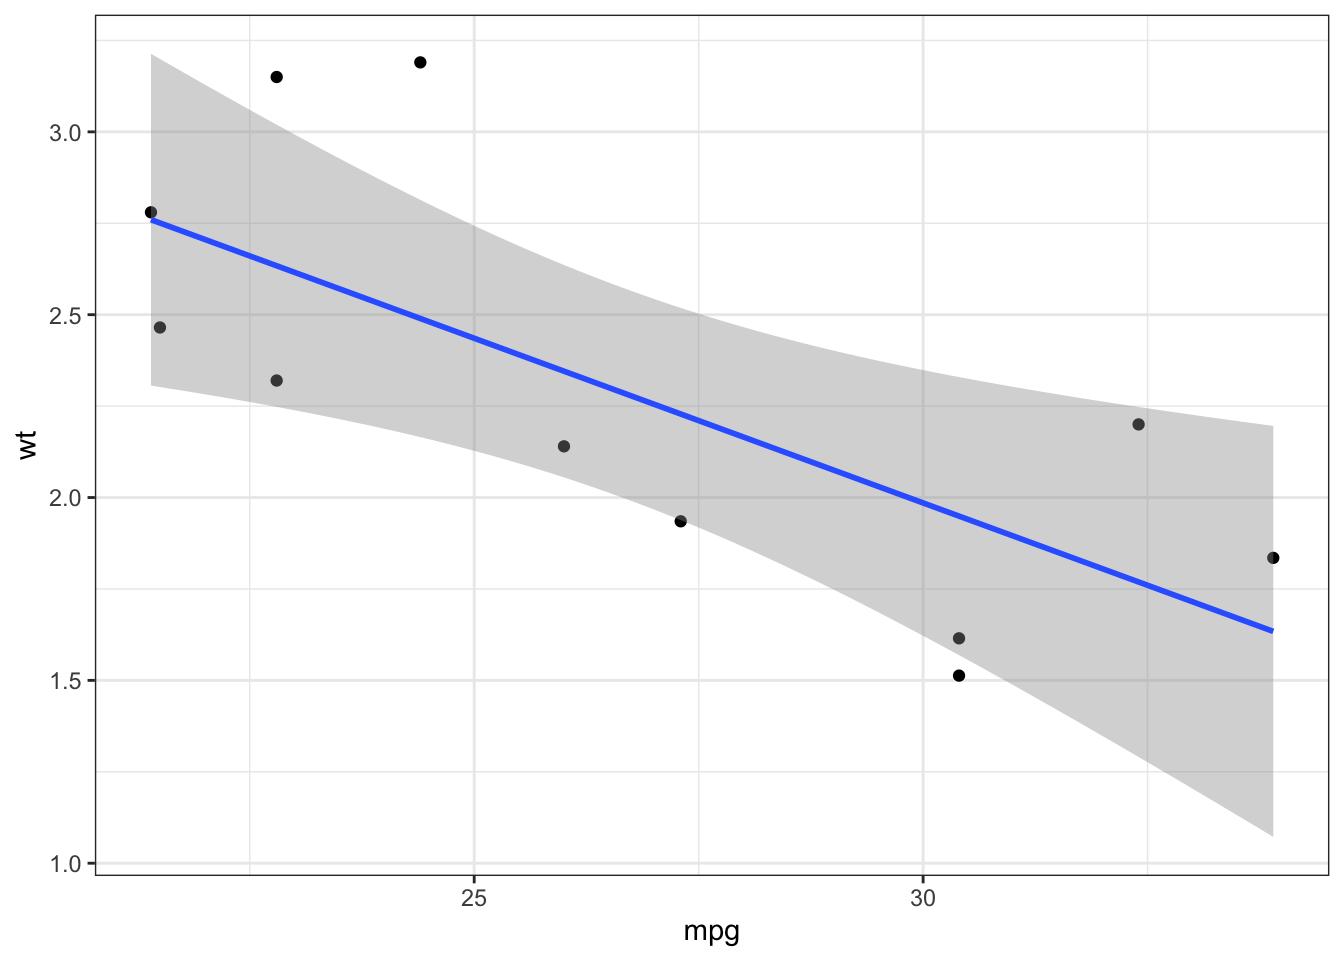
\includegraphics{_main_files/figure-latex/unnamed-chunk-78-1.pdf}

\begin{Shaded}
\begin{Highlighting}[]
\NormalTok{p[[}\DecValTok{3}\NormalTok{]]}
\end{Highlighting}
\end{Shaded}

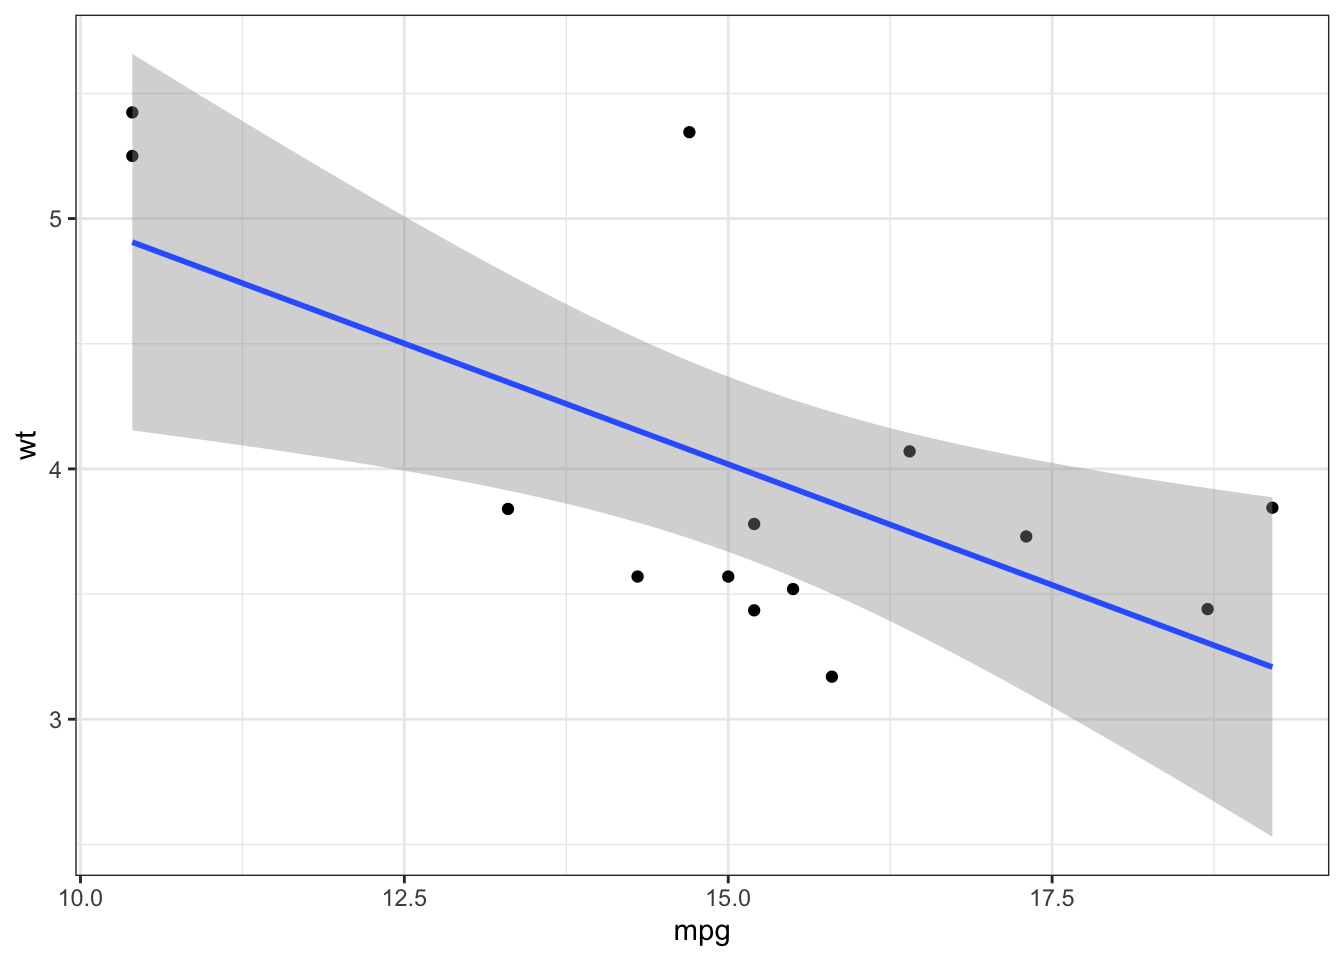
\includegraphics{_main_files/figure-latex/unnamed-chunk-78-2.pdf}

Combining the package \texttt{broom} with iterative model fitting is particularly useful:

\begin{Shaded}
\begin{Highlighting}[]
\FunctionTok{library}\NormalTok{(broom)}
\NormalTok{mtcars\_lst }\SpecialCharTok{\%\textgreater{}\%}
  \FunctionTok{map}\NormalTok{(}\SpecialCharTok{\textasciitilde{}} \FunctionTok{lm}\NormalTok{(mpg }\SpecialCharTok{\textasciitilde{}}\NormalTok{ gear, }\AttributeTok{data =}\NormalTok{ .x)) }\SpecialCharTok{\%\textgreater{}\%}
  \FunctionTok{map}\NormalTok{(glance) }\SpecialCharTok{\%\textgreater{}\%}
  \FunctionTok{bind\_rows}\NormalTok{()}
\end{Highlighting}
\end{Shaded}

\begin{verbatim}
## # A tibble: 3 x 12
##   r.squared adj.r.~1 sigma stati~2 p.value    df logLik   AIC
##       <dbl>    <dbl> <dbl>   <dbl>   <dbl> <dbl>  <dbl> <dbl>
## 1 0.115       0.0163  4.47 1.17e+0   0.308     1  -31.0  68.0
## 2 0.0000902  -0.200   1.59 4.51e-4   0.984     1  -12.0  30.0
## 3 0.00246    -0.0807  2.66 2.97e-2   0.866     1  -32.5  71.0
## # ... with 4 more variables: BIC <dbl>, deviance <dbl>,
## #   df.residual <int>, nobs <int>, and abbreviated variable
## #   names 1: adj.r.squared, 2: statistic
\end{verbatim}

Using \texttt{lapply()} instead:

\begin{Shaded}
\begin{Highlighting}[]
\FunctionTok{lapply}\NormalTok{(mtcars\_lst, }\ControlFlowTok{function}\NormalTok{(x) }\FunctionTok{lm}\NormalTok{(mpg }\SpecialCharTok{\textasciitilde{}}\NormalTok{ gear, }\AttributeTok{data =}\NormalTok{ x)) }\SpecialCharTok{\%\textgreater{}\%}
  \FunctionTok{lapply}\NormalTok{(glance) }\SpecialCharTok{\%\textgreater{}\%} \FunctionTok{bind\_rows}\NormalTok{()}
\end{Highlighting}
\end{Shaded}

\begin{verbatim}
## # A tibble: 3 x 12
##   r.squared adj.r.~1 sigma stati~2 p.value    df logLik   AIC
##       <dbl>    <dbl> <dbl>   <dbl>   <dbl> <dbl>  <dbl> <dbl>
## 1 0.115       0.0163  4.47 1.17e+0   0.308     1  -31.0  68.0
## 2 0.0000902  -0.200   1.59 4.51e-4   0.984     1  -12.0  30.0
## 3 0.00246    -0.0807  2.66 2.97e-2   0.866     1  -32.5  71.0
## # ... with 4 more variables: BIC <dbl>, deviance <dbl>,
## #   df.residual <int>, nobs <int>, and abbreviated variable
## #   names 1: adj.r.squared, 2: statistic
\end{verbatim}

The \texttt{map()} function can also be used to extract elements:

\begin{Shaded}
\begin{Highlighting}[]
\NormalTok{mtcars\_lst }\SpecialCharTok{\%\textgreater{}\%} \FunctionTok{map}\NormalTok{(}\StringTok{\textquotesingle{}CAR\textquotesingle{}}\NormalTok{)}
\end{Highlighting}
\end{Shaded}

\begin{verbatim}
## [[1]]
##  [1] "Datsun 710"     "Merc 240D"      "Merc 230"      
##  [4] "Fiat 128"       "Honda Civic"    "Toyota Corolla"
##  [7] "Toyota Corona"  "Fiat X1-9"      "Porsche 914-2" 
## [10] "Lotus Europa"   "Volvo 142E"    
## 
## [[2]]
## [1] "Mazda RX4"      "Mazda RX4 Wag"  "Hornet 4 Drive"
## [4] "Valiant"        "Merc 280"       "Merc 280C"     
## [7] "Ferrari Dino"  
## 
## [[3]]
##  [1] "Hornet Sportabout"   "Duster 360"         
##  [3] "Merc 450SE"          "Merc 450SL"         
##  [5] "Merc 450SLC"         "Cadillac Fleetwood" 
##  [7] "Lincoln Continental" "Chrysler Imperial"  
##  [9] "Dodge Challenger"    "AMC Javelin"        
## [11] "Camaro Z28"          "Pontiac Firebird"   
## [13] "Ford Pantera L"      "Maserati Bora"
\end{verbatim}

\begin{Shaded}
\begin{Highlighting}[]
\NormalTok{mtcars\_lst }\SpecialCharTok{\%\textgreater{}\%}
  \FunctionTok{map}\NormalTok{(}\SpecialCharTok{\textasciitilde{}} \FunctionTok{lm}\NormalTok{(mpg }\SpecialCharTok{\textasciitilde{}}\NormalTok{ gear, }\AttributeTok{data =}\NormalTok{ .x)) }\SpecialCharTok{\%\textgreater{}\%}
  \FunctionTok{map}\NormalTok{(coef) }\SpecialCharTok{\%\textgreater{}\%}
  \FunctionTok{map\_dbl}\NormalTok{(}\DecValTok{2}\NormalTok{)}
\end{Highlighting}
\end{Shaded}

\begin{verbatim}
## [1]  2.83125 -0.02000  0.17500
\end{verbatim}

\hypertarget{iterating-over-vectors}{%
\section{Iterating over vectors}\label{iterating-over-vectors}}

Let's say we have a vector with missing values:

\begin{Shaded}
\begin{Highlighting}[]
\NormalTok{x }\OtherTok{\textless{}{-}} \FunctionTok{c}\NormalTok{(}\DecValTok{3}\NormalTok{, }\DecValTok{2}\NormalTok{, }\ConstantTok{NA}\NormalTok{, }\DecValTok{2}\NormalTok{, }\DecValTok{1}\NormalTok{, }\DecValTok{4}\NormalTok{, }\DecValTok{2}\NormalTok{, }\ConstantTok{NA}\NormalTok{, }\DecValTok{2}\NormalTok{, }\ConstantTok{NA}\NormalTok{)}
\NormalTok{x}
\end{Highlighting}
\end{Shaded}

\begin{verbatim}
##  [1]  3  2 NA  2  1  4  2 NA  2 NA
\end{verbatim}

Filling the missing values is easy with iteration over the length of the vector:

\begin{Shaded}
\begin{Highlighting}[]
\NormalTok{x }\SpecialCharTok{\%\textgreater{}\%} \FunctionTok{map\_dbl}\NormalTok{(}\SpecialCharTok{\textasciitilde{}} \FunctionTok{replace}\NormalTok{(., }\FunctionTok{is.na}\NormalTok{(.x), }\DecValTok{0}\NormalTok{))}
\end{Highlighting}
\end{Shaded}

\begin{verbatim}
##  [1] 3 2 0 2 1 4 2 0 2 0
\end{verbatim}

Or if we want to replace the missing values with the mean:

\begin{Shaded}
\begin{Highlighting}[]
\NormalTok{x }\SpecialCharTok{\%\textgreater{}\%} \FunctionTok{map\_dbl}\NormalTok{(}\SpecialCharTok{\textasciitilde{}} \FunctionTok{replace}\NormalTok{(., }\FunctionTok{is.na}\NormalTok{(.x), }\FunctionTok{mean}\NormalTok{(x, }\AttributeTok{na.rm =} \ConstantTok{TRUE}\NormalTok{)))}
\end{Highlighting}
\end{Shaded}

\begin{verbatim}
##  [1] 3.000000 2.000000 2.285714 2.000000 1.000000 4.000000
##  [7] 2.000000 2.285714 2.000000 2.285714
\end{verbatim}

This can of course be done with a for loop instead:

\begin{Shaded}
\begin{Highlighting}[]
\ControlFlowTok{for}\NormalTok{ (i }\ControlFlowTok{in} \FunctionTok{seq\_along}\NormalTok{(x))\{}
  \ControlFlowTok{if}\NormalTok{ (}\FunctionTok{is.na}\NormalTok{(x[i]) }\SpecialCharTok{==} \ConstantTok{TRUE}\NormalTok{)\{}
\NormalTok{    x[i] }\OtherTok{\textless{}{-}} \FunctionTok{mean}\NormalTok{(x, }\AttributeTok{na.rm =} \ConstantTok{TRUE}\NormalTok{)}
\NormalTok{  \}}
\NormalTok{\}}

\NormalTok{x}
\end{Highlighting}
\end{Shaded}

\begin{verbatim}
##  [1] 3.000000 2.000000 2.285714 2.000000 1.000000 4.000000
##  [7] 2.000000 2.285714 2.000000 2.285714
\end{verbatim}

Note that \texttt{seq\_along(x)} prints the indices along the length of the vector, as if to write \texttt{1:length(x)}.

Iterating over a vector of characters requires \texttt{map\_chr()} to get the character vector back, but the syntax is the same:

\begin{Shaded}
\begin{Highlighting}[]
\NormalTok{z }\OtherTok{\textless{}{-}} \FunctionTok{c}\NormalTok{(}\StringTok{\textquotesingle{}Brian\textquotesingle{}}\NormalTok{, }\StringTok{\textquotesingle{}Connor\textquotesingle{}}\NormalTok{, }\StringTok{\textquotesingle{}Harry\textquotesingle{}}\NormalTok{, }\StringTok{\textquotesingle{}Sonny\textquotesingle{}}\NormalTok{)}
\FunctionTok{map\_chr}\NormalTok{(z, }\SpecialCharTok{\textasciitilde{}} \FunctionTok{paste0}\NormalTok{(.x, }\StringTok{\textquotesingle{}\_NAME\textquotesingle{}}\NormalTok{))}
\end{Highlighting}
\end{Shaded}

\begin{verbatim}
## [1] "Brian_NAME"  "Connor_NAME" "Harry_NAME"  "Sonny_NAME"
\end{verbatim}

\begin{Shaded}
\begin{Highlighting}[]
\NormalTok{out }\OtherTok{\textless{}{-}} \FunctionTok{character}\NormalTok{(}\FunctionTok{length}\NormalTok{(z))}
\ControlFlowTok{for}\NormalTok{ (i }\ControlFlowTok{in} \FunctionTok{seq\_along}\NormalTok{(z))\{}
\NormalTok{  out[i] }\OtherTok{\textless{}{-}} \FunctionTok{paste0}\NormalTok{(z[i], }\StringTok{\textquotesingle{}\_NAME\textquotesingle{}}\NormalTok{)}
\NormalTok{\}}
\NormalTok{out}
\end{Highlighting}
\end{Shaded}

\begin{verbatim}
## [1] "Brian_NAME"  "Connor_NAME" "Harry_NAME"  "Sonny_NAME"
\end{verbatim}

In particular cases where the output is printed out, as in the case of \texttt{print()} and \texttt{cat()}, we may end up echoing both the return values and the output list when using \texttt{map()}. To that end, \texttt{walk()} is used to avoid showing the result twice:

\begin{Shaded}
\begin{Highlighting}[]
\FunctionTok{walk}\NormalTok{(z, }\SpecialCharTok{\textasciitilde{}} \FunctionTok{print}\NormalTok{(}\FunctionTok{paste0}\NormalTok{(.x, }\StringTok{\textquotesingle{}\_NAME\textquotesingle{}}\NormalTok{)))}
\end{Highlighting}
\end{Shaded}

\begin{verbatim}
## [1] "Brian_NAME"
## [1] "Connor_NAME"
## [1] "Harry_NAME"
## [1] "Sonny_NAME"
\end{verbatim}

\hypertarget{iterating-with-two-inputs}{%
\section{Iterating with two inputs}\label{iterating-with-two-inputs}}

In contrast to every solution so far, there's a case to be made about iterating over multiple inputs. For that purpose, \texttt{purrr:map2} does the job.

\begin{Shaded}
\begin{Highlighting}[]
\NormalTok{x }\OtherTok{\textless{}{-}} \FunctionTok{c}\NormalTok{(}\DecValTok{2}\NormalTok{, }\DecValTok{4}\NormalTok{, }\DecValTok{2}\NormalTok{, }\DecValTok{5}\NormalTok{)}
\NormalTok{y }\OtherTok{\textless{}{-}} \FunctionTok{c}\NormalTok{(}\DecValTok{2}\NormalTok{, }\DecValTok{6}\NormalTok{, }\DecValTok{3}\NormalTok{, }\DecValTok{1}\NormalTok{)}
\FunctionTok{map2\_dbl}\NormalTok{(x, y, sum)}
\end{Highlighting}
\end{Shaded}

\begin{verbatim}
## [1]  4 10  5  6
\end{verbatim}

\begin{Shaded}
\begin{Highlighting}[]
\FunctionTok{map2\_chr}\NormalTok{(x, y, }\SpecialCharTok{\textasciitilde{}} \FunctionTok{str\_glue}\NormalTok{(}\StringTok{\textquotesingle{}The sum of \{.x\} and \{.y\} is \{sum(.x, .y)\}\textquotesingle{}}\NormalTok{))}
\end{Highlighting}
\end{Shaded}

\begin{verbatim}
## [1] "The sum of 2 and 2 is 4"  "The sum of 4 and 6 is 10"
## [3] "The sum of 2 and 3 is 5"  "The sum of 5 and 1 is 6"
\end{verbatim}

Note that the iteration occurs at the \emph{i}th position of each vector.

The intuition behind \texttt{map2()} is straightforward and is illustrated by the equivalent for loop:

\begin{Shaded}
\begin{Highlighting}[]
\NormalTok{result }\OtherTok{\textless{}{-}} \FunctionTok{numeric}\NormalTok{(}\FunctionTok{length}\NormalTok{(x))}
\ControlFlowTok{for}\NormalTok{ (i }\ControlFlowTok{in} \FunctionTok{seq\_along}\NormalTok{(x))\{}
\NormalTok{  result[i] }\OtherTok{\textless{}{-}} \FunctionTok{sum}\NormalTok{(x[i], y[i])}
\NormalTok{\}}
\NormalTok{result}
\end{Highlighting}
\end{Shaded}

\begin{verbatim}
## [1]  4 10  5  6
\end{verbatim}

One quirk with \texttt{map2()} is that it recycles the input:

\begin{Shaded}
\begin{Highlighting}[]
\FunctionTok{map2\_chr}\NormalTok{(}\StringTok{\textquotesingle{}My name is \textquotesingle{}}\NormalTok{, }\FunctionTok{c}\NormalTok{(}\StringTok{\textquotesingle{}Brian\textquotesingle{}}\NormalTok{, }\StringTok{\textquotesingle{}Connor\textquotesingle{}}\NormalTok{), str\_c)}
\end{Highlighting}
\end{Shaded}

\begin{verbatim}
## [1] "My name is Brian"  "My name is Connor"
\end{verbatim}

Suppose a dataset such as this:

\begin{Shaded}
\begin{Highlighting}[]
\NormalTok{z }\OtherTok{\textless{}{-}} \FunctionTok{tibble}\NormalTok{(}\AttributeTok{A =}\NormalTok{ x, }\AttributeTok{B =}\NormalTok{ y)}
\NormalTok{z}
\end{Highlighting}
\end{Shaded}

\begin{verbatim}
## # A tibble: 4 x 2
##       A     B
##   <dbl> <dbl>
## 1     2     2
## 2     4     6
## 3     2     3
## 4     5     1
\end{verbatim}

There may be cases where we want to create a new column using \texttt{mutate()} which results from a transformation of the \texttt{A} and \texttt{B} columns at each row.

First, see why the following does not work in creating a column \texttt{C} which takes the higher value between \texttt{A} and \texttt{B} at each row:

\begin{Shaded}
\begin{Highlighting}[]
\NormalTok{z }\SpecialCharTok{\%\textgreater{}\%} \FunctionTok{mutate}\NormalTok{(}\AttributeTok{C =} \FunctionTok{max}\NormalTok{(A, B))}
\end{Highlighting}
\end{Shaded}

\begin{verbatim}
## # A tibble: 4 x 3
##       A     B     C
##   <dbl> <dbl> <dbl>
## 1     2     2     6
## 2     4     6     6
## 3     2     3     6
## 4     5     1     6
\end{verbatim}

Using \texttt{map2()}, however, this does work:

\begin{Shaded}
\begin{Highlighting}[]
\NormalTok{z }\SpecialCharTok{\%\textgreater{}\%} \FunctionTok{mutate}\NormalTok{(}\AttributeTok{C =} \FunctionTok{map2\_dbl}\NormalTok{(A, B, max))}
\end{Highlighting}
\end{Shaded}

\begin{verbatim}
## # A tibble: 4 x 3
##       A     B     C
##   <dbl> <dbl> <dbl>
## 1     2     2     2
## 2     4     6     6
## 3     2     3     3
## 4     5     1     5
\end{verbatim}

Other families of \texttt{map2()} works normally in this context, for example, if we want to check whether the sum of \texttt{A} and \texttt{B} at each row is an even number:

\begin{Shaded}
\begin{Highlighting}[]
\NormalTok{z }\SpecialCharTok{\%\textgreater{}\%} \FunctionTok{mutate}\NormalTok{(}\AttributeTok{C =} \FunctionTok{map2\_lgl}\NormalTok{(A, B, }\SpecialCharTok{\textasciitilde{}}\NormalTok{ (.x }\SpecialCharTok{+}\NormalTok{ .y) }\SpecialCharTok{\%\%} \DecValTok{2} \SpecialCharTok{==} \DecValTok{0}\NormalTok{))}
\end{Highlighting}
\end{Shaded}

\begin{verbatim}
## # A tibble: 4 x 3
##       A     B C    
##   <dbl> <dbl> <lgl>
## 1     2     2 TRUE 
## 2     4     6 TRUE 
## 3     2     3 FALSE
## 4     5     1 TRUE
\end{verbatim}

When there are more than 2 inputs, we can use \texttt{pmap()} instead; this function takes a list of the inputs instead:

\begin{Shaded}
\begin{Highlighting}[]
\NormalTok{w }\OtherTok{\textless{}{-}} \FunctionTok{c}\NormalTok{(}\DecValTok{4}\NormalTok{, }\DecValTok{2}\NormalTok{, }\DecValTok{3}\NormalTok{, }\DecValTok{1}\NormalTok{)}
\FunctionTok{pmap\_dbl}\NormalTok{(}\FunctionTok{list}\NormalTok{(x, y, w), sum)}
\end{Highlighting}
\end{Shaded}

\begin{verbatim}
## [1]  8 12  8  7
\end{verbatim}

\begin{Shaded}
\begin{Highlighting}[]
\NormalTok{z }\OtherTok{\textless{}{-}} \FunctionTok{tibble}\NormalTok{(}\AttributeTok{A =}\NormalTok{ x, }\AttributeTok{B =}\NormalTok{ y, }\AttributeTok{C =}\NormalTok{ w)}
\NormalTok{z}
\end{Highlighting}
\end{Shaded}

\begin{verbatim}
## # A tibble: 4 x 3
##       A     B     C
##   <dbl> <dbl> <dbl>
## 1     2     2     4
## 2     4     6     2
## 3     2     3     3
## 4     5     1     1
\end{verbatim}

\begin{Shaded}
\begin{Highlighting}[]
\NormalTok{z }\SpecialCharTok{\%\textgreater{}\%} \FunctionTok{mutate}\NormalTok{(}\AttributeTok{v =} \FunctionTok{pmap\_lgl}\NormalTok{(}\FunctionTok{list}\NormalTok{(A, B, C), }\SpecialCharTok{\textasciitilde{}} \FunctionTok{sum}\NormalTok{(.) }\SpecialCharTok{\%\%} \DecValTok{2} \SpecialCharTok{==} \DecValTok{0}\NormalTok{))}
\end{Highlighting}
\end{Shaded}

\begin{verbatim}
## # A tibble: 4 x 4
##       A     B     C v    
##   <dbl> <dbl> <dbl> <lgl>
## 1     2     2     4 TRUE 
## 2     4     6     2 TRUE 
## 3     2     3     3 TRUE 
## 4     5     1     1 FALSE
\end{verbatim}

Using the notation for anonymous functions instead:

\begin{Shaded}
\begin{Highlighting}[]
\NormalTok{z }\SpecialCharTok{\%\textgreater{}\%} \FunctionTok{mutate}\NormalTok{(}\AttributeTok{v =} \FunctionTok{pmap\_lgl}\NormalTok{(}\FunctionTok{list}\NormalTok{(A, B, C), }\SpecialCharTok{\textasciitilde{}} \FunctionTok{sum}\NormalTok{(..}\DecValTok{1} \SpecialCharTok{+}\NormalTok{ ..}\DecValTok{2} \SpecialCharTok{+}\NormalTok{ ..}\DecValTok{3}\NormalTok{) }\SpecialCharTok{\%\%} \DecValTok{2} \SpecialCharTok{==} \DecValTok{0}\NormalTok{))}
\end{Highlighting}
\end{Shaded}

\begin{verbatim}
## # A tibble: 4 x 4
##       A     B     C v    
##   <dbl> <dbl> <dbl> <lgl>
## 1     2     2     4 TRUE 
## 2     4     6     2 TRUE 
## 3     2     3     3 TRUE 
## 4     5     1     1 FALSE
\end{verbatim}

\hypertarget{iterating-over-indices-and-names}{%
\section{Iterating over indices and names}\label{iterating-over-indices-and-names}}

A related function is \texttt{imap()} and its variants, which is analogous to looping over numeric indices, such as in the case of \texttt{for\ (i\ in\ seq\_along(x))}. That is, it applies a function over an input and its corresponding index. For example:

\begin{Shaded}
\begin{Highlighting}[]
\NormalTok{x }\OtherTok{\textless{}{-}} \FunctionTok{c}\NormalTok{(}\DecValTok{2}\NormalTok{, }\DecValTok{4}\NormalTok{, }\DecValTok{2}\NormalTok{, }\DecValTok{5}\NormalTok{)}
\FunctionTok{imap\_chr}\NormalTok{(x, }\SpecialCharTok{\textasciitilde{}} \FunctionTok{paste0}\NormalTok{(}\StringTok{\textquotesingle{}The index \textquotesingle{}}\NormalTok{, .y, }\StringTok{\textquotesingle{} number in x is \textquotesingle{}}\NormalTok{, .x))}
\end{Highlighting}
\end{Shaded}

\begin{verbatim}
## [1] "The index 1 number in x is 2"
## [2] "The index 2 number in x is 4"
## [3] "The index 3 number in x is 2"
## [4] "The index 4 number in x is 5"
\end{verbatim}

Without using \texttt{purrr}, this is equivalent to the for loop:

\begin{Shaded}
\begin{Highlighting}[]
\NormalTok{out }\OtherTok{\textless{}{-}} \FunctionTok{character}\NormalTok{(}\FunctionTok{length}\NormalTok{(x))}
\ControlFlowTok{for}\NormalTok{ (i }\ControlFlowTok{in} \FunctionTok{seq\_along}\NormalTok{(x))\{}
\NormalTok{  out[i] }\OtherTok{\textless{}{-}} \FunctionTok{paste0}\NormalTok{(}\StringTok{\textquotesingle{}The index \textquotesingle{}}\NormalTok{, i, }\StringTok{\textquotesingle{} number in x is \textquotesingle{}}\NormalTok{, x[i])}
\NormalTok{\}}
\NormalTok{out}
\end{Highlighting}
\end{Shaded}

\begin{verbatim}
## [1] "The index 1 number in x is 2"
## [2] "The index 2 number in x is 4"
## [3] "The index 3 number in x is 2"
## [4] "The index 4 number in x is 5"
\end{verbatim}

\texttt{imap} also works with names instead of indices, if required:

\begin{Shaded}
\begin{Highlighting}[]
\FunctionTok{names}\NormalTok{(x) }\OtherTok{\textless{}{-}} \FunctionTok{c}\NormalTok{(}\StringTok{\textquotesingle{}A\textquotesingle{}}\NormalTok{, }\StringTok{\textquotesingle{}B\textquotesingle{}}\NormalTok{, }\StringTok{\textquotesingle{}C\textquotesingle{}}\NormalTok{, }\StringTok{\textquotesingle{}D\textquotesingle{}}\NormalTok{)}
\FunctionTok{imap\_lgl}\NormalTok{(x, }\SpecialCharTok{\textasciitilde{}} \ControlFlowTok{if}\NormalTok{(.y }\SpecialCharTok{\%in\%} \FunctionTok{c}\NormalTok{(}\StringTok{\textquotesingle{}A\textquotesingle{}}\NormalTok{, }\StringTok{\textquotesingle{}C\textquotesingle{}}\NormalTok{)) }\ConstantTok{TRUE} \ControlFlowTok{else} \ConstantTok{FALSE}\NormalTok{)}
\end{Highlighting}
\end{Shaded}

\begin{verbatim}
##     A     B     C     D 
##  TRUE FALSE  TRUE FALSE
\end{verbatim}

The equivalent expression in the form of a for loop is as follows:

\begin{Shaded}
\begin{Highlighting}[]
\NormalTok{out }\OtherTok{\textless{}{-}} \FunctionTok{logical}\NormalTok{()}
\ControlFlowTok{for}\NormalTok{ (i }\ControlFlowTok{in} \FunctionTok{names}\NormalTok{(x))\{}
  \ControlFlowTok{if}\NormalTok{(i }\SpecialCharTok{\%in\%} \FunctionTok{c}\NormalTok{(}\StringTok{\textquotesingle{}A\textquotesingle{}}\NormalTok{, }\StringTok{\textquotesingle{}C\textquotesingle{}}\NormalTok{))\{}
\NormalTok{    out[i] }\OtherTok{\textless{}{-}} \ConstantTok{TRUE}
\NormalTok{  \} }\ControlFlowTok{else}\NormalTok{ \{}
\NormalTok{    out[i] }\OtherTok{\textless{}{-}} \ConstantTok{FALSE}
\NormalTok{  \}}
\NormalTok{\}}
\NormalTok{out}
\end{Highlighting}
\end{Shaded}

\begin{verbatim}
##     A     B     C     D 
##  TRUE FALSE  TRUE FALSE
\end{verbatim}

Therefore, we see clearly that the two uses of \texttt{imap()} - iterating over indices and over names - is equivalent to \texttt{for\ (i\ in\ seq\_along(x))} and \texttt{for\ (i\ in\ names(x))}, respectively.

\hypertarget{handling-errors-within-purrr}{%
\section{\texorpdfstring{Handling errors within \texttt{purrr}}{Handling errors within purrr}}\label{handling-errors-within-purrr}}

Let's return to the \texttt{mtcars} dataset, specifically after we split the tibble into a list based on \texttt{group\_split(cyl)}.

\begin{Shaded}
\begin{Highlighting}[]
\NormalTok{mtcars\_lst }\OtherTok{\textless{}{-}}\NormalTok{ mtcars }\SpecialCharTok{\%\textgreater{}\%} \FunctionTok{group\_split}\NormalTok{(cyl)}
\end{Highlighting}
\end{Shaded}

For one of the elements of the list, I'm filling the \texttt{gear} column with missing values:

\begin{Shaded}
\begin{Highlighting}[]
\NormalTok{mtcars\_lst[[}\DecValTok{2}\NormalTok{]] }\OtherTok{\textless{}{-}}\NormalTok{ mtcars\_lst[[}\DecValTok{2}\NormalTok{]] }\SpecialCharTok{\%\textgreater{}\%} \FunctionTok{mutate}\NormalTok{(}\AttributeTok{gear =} \ConstantTok{NA}\NormalTok{)}
\NormalTok{mtcars\_lst[[}\DecValTok{2}\NormalTok{]]}
\end{Highlighting}
\end{Shaded}

\begin{verbatim}
## # A tibble: 7 x 12
##   CAR     mpg   cyl  disp    hp  drat    wt  qsec    vs    am
##   <chr> <dbl> <dbl> <dbl> <dbl> <dbl> <dbl> <dbl> <dbl> <dbl>
## 1 Mazd~  21       6  160    110  3.9   2.62  16.5     0     1
## 2 Mazd~  21       6  160    110  3.9   2.88  17.0     0     1
## 3 Horn~  21.4     6  258    110  3.08  3.22  19.4     1     0
## 4 Vali~  18.1     6  225    105  2.76  3.46  20.2     1     0
## 5 Merc~  19.2     6  168.   123  3.92  3.44  18.3     1     0
## 6 Merc~  17.8     6  168.   123  3.92  3.44  18.9     1     0
## 7 Ferr~  19.7     6  145    175  3.62  2.77  15.5     0     1
## # ... with 2 more variables: gear <dbl>, carb <dbl>
\end{verbatim}

Now, if I were to try and fit a linear model using \texttt{lm(mpg\ \textasciitilde{}\ wt)} iteratively over the \texttt{mtcars\_lst}, it will fail at the second element as the \texttt{wt} values are all missing.

\begin{Shaded}
\begin{Highlighting}[]
\NormalTok{mtcars\_lst }\SpecialCharTok{\%\textgreater{}\%}
  \FunctionTok{map}\NormalTok{(}\SpecialCharTok{\textasciitilde{}} \FunctionTok{lm}\NormalTok{(mpg }\SpecialCharTok{\textasciitilde{}}\NormalTok{ gear, }\AttributeTok{data =}\NormalTok{ .x)) }\SpecialCharTok{\%\textgreater{}\%}
  \FunctionTok{map}\NormalTok{(coef) }\SpecialCharTok{\%\textgreater{}\%}
  \FunctionTok{map\_dbl}\NormalTok{(}\DecValTok{2}\NormalTok{) }\CommentTok{\# returns an error}
\end{Highlighting}
\end{Shaded}

This is inconvenient in many cases as ideally we'd want to skip over the iteration at which the function fails and get the rest of the results. Thankfully this can be done using \texttt{possibly()}; note the second element in the output where the \texttt{lm()} function would've failed:

\begin{Shaded}
\begin{Highlighting}[]
\FunctionTok{map}\NormalTok{(mtcars\_lst, }\FunctionTok{possibly}\NormalTok{(}\SpecialCharTok{\textasciitilde{}} \FunctionTok{lm}\NormalTok{(mpg }\SpecialCharTok{\textasciitilde{}}\NormalTok{ gear, }\AttributeTok{data =}\NormalTok{ .x), }\AttributeTok{otherwise =} \ConstantTok{NA}\NormalTok{))}
\end{Highlighting}
\end{Shaded}

\begin{verbatim}
## [[1]]
## 
## Call:
## lm(formula = mpg ~ gear, data = .x)
## 
## Coefficients:
## (Intercept)         gear  
##      15.081        2.831  
## 
## 
## [[2]]
## [1] NA
## 
## [[3]]
## 
## Call:
## lm(formula = mpg ~ gear, data = .x)
## 
## Coefficients:
## (Intercept)         gear  
##      14.525        0.175
\end{verbatim}

The second argument within \texttt{otherwise\ =} argument within \texttt{possibly()}, where we wrapped the iterative function, provides an alternative solution in case the function fails. As we can see above, the second element of the output corresponds to \texttt{NA} and the iteration continued after.

Using \texttt{purrr::keep()} I can select for the elements that did not fail:

\begin{Shaded}
\begin{Highlighting}[]
\FunctionTok{map}\NormalTok{(mtcars\_lst, }\FunctionTok{possibly}\NormalTok{(}\SpecialCharTok{\textasciitilde{}} \FunctionTok{lm}\NormalTok{(mpg }\SpecialCharTok{\textasciitilde{}}\NormalTok{ gear, }\AttributeTok{data =}\NormalTok{ .x), }\AttributeTok{otherwise =} \ConstantTok{NA}\NormalTok{)) }\SpecialCharTok{\%\textgreater{}\%} 
  \FunctionTok{keep}\NormalTok{(}\SpecialCharTok{\textasciitilde{}} \SpecialCharTok{!}\FunctionTok{is.na}\NormalTok{(.x) }\SpecialCharTok{\%\textgreater{}\%} \FunctionTok{all}\NormalTok{())}
\end{Highlighting}
\end{Shaded}

\begin{verbatim}
## [[1]]
## 
## Call:
## lm(formula = mpg ~ gear, data = .x)
## 
## Coefficients:
## (Intercept)         gear  
##      15.081        2.831  
## 
## 
## [[2]]
## 
## Call:
## lm(formula = mpg ~ gear, data = .x)
## 
## Coefficients:
## (Intercept)         gear  
##      14.525        0.175
\end{verbatim}

Of course this is the same as running the first \texttt{map()} function wrapped around \texttt{possibly()} and then running \texttt{result{[}-which(is.na(result){]}}.

Sometimes it's not useful to keep the failed element in the first place, so setting \texttt{otherwise\ =\ NULL} within \texttt{possibly()} works too. Afterwards, removing the empty element (i.e., \texttt{NULL}) is done using \texttt{purrr::compact()}.

\begin{Shaded}
\begin{Highlighting}[]
\FunctionTok{map}\NormalTok{(mtcars\_lst, }\FunctionTok{possibly}\NormalTok{(}\SpecialCharTok{\textasciitilde{}} \FunctionTok{lm}\NormalTok{(mpg }\SpecialCharTok{\textasciitilde{}}\NormalTok{ gear, }\AttributeTok{data =}\NormalTok{ .x), }\AttributeTok{otherwise =} \ConstantTok{NULL}\NormalTok{)) }\SpecialCharTok{\%\textgreater{}\%}
  \FunctionTok{compact}\NormalTok{()}
\end{Highlighting}
\end{Shaded}

\begin{verbatim}
## [[1]]
## 
## Call:
## lm(formula = mpg ~ gear, data = .x)
## 
## Coefficients:
## (Intercept)         gear  
##      15.081        2.831  
## 
## 
## [[2]]
## 
## Call:
## lm(formula = mpg ~ gear, data = .x)
## 
## Coefficients:
## (Intercept)         gear  
##      14.525        0.175
\end{verbatim}

Instead of discarding the iteration where the function failed, we could also catch the error by using \texttt{safely()} instead. This returns a nested list as such:

\begin{Shaded}
\begin{Highlighting}[]
\FunctionTok{map}\NormalTok{(mtcars\_lst, }\FunctionTok{safely}\NormalTok{(}\SpecialCharTok{\textasciitilde{}} \FunctionTok{lm}\NormalTok{(mpg }\SpecialCharTok{\textasciitilde{}}\NormalTok{ gear, }\AttributeTok{data =}\NormalTok{ .x)))}
\end{Highlighting}
\end{Shaded}

\begin{verbatim}
## [[1]]
## [[1]]$result
## 
## Call:
## lm(formula = mpg ~ gear, data = .x)
## 
## Coefficients:
## (Intercept)         gear  
##      15.081        2.831  
## 
## 
## [[1]]$error
## NULL
## 
## 
## [[2]]
## [[2]]$result
## NULL
## 
## [[2]]$error
## <simpleError in lm.fit(x, y, offset = offset, singular.ok = singular.ok, ...): 0 (non-NA) cases>
## 
## 
## [[3]]
## [[3]]$result
## 
## Call:
## lm(formula = mpg ~ gear, data = .x)
## 
## Coefficients:
## (Intercept)         gear  
##      14.525        0.175  
## 
## 
## [[3]]$error
## NULL
\end{verbatim}

We could also just pull the \texttt{error} terms and throw away the empty \texttt{NULL} elements:

\begin{Shaded}
\begin{Highlighting}[]
\FunctionTok{map}\NormalTok{(mtcars\_lst, }\FunctionTok{safely}\NormalTok{(}\SpecialCharTok{\textasciitilde{}} \FunctionTok{lm}\NormalTok{(mpg }\SpecialCharTok{\textasciitilde{}}\NormalTok{ gear, }\AttributeTok{data =}\NormalTok{ .x))) }\SpecialCharTok{\%\textgreater{}\%} \FunctionTok{map}\NormalTok{(}\StringTok{\textquotesingle{}error\textquotesingle{}}\NormalTok{) }\SpecialCharTok{\%\textgreater{}\%}
  \FunctionTok{compact}\NormalTok{()}
\end{Highlighting}
\end{Shaded}

\begin{verbatim}
## [[1]]
## <simpleError in lm.fit(x, y, offset = offset, singular.ok = singular.ok, ...): 0 (non-NA) cases>
\end{verbatim}

In a traditional for loop without \texttt{purrr}, a solution could be to use \texttt{tryCatch()} with \texttt{next}. Below returns the iteration with the error as \texttt{NULL} as was the case with \texttt{possibly(...,\ otherwise\ =\ NULL)}.

\begin{Shaded}
\begin{Highlighting}[]
\NormalTok{mod }\OtherTok{\textless{}{-}} \FunctionTok{list}\NormalTok{()}
\ControlFlowTok{for}\NormalTok{ (i }\ControlFlowTok{in} \FunctionTok{seq\_along}\NormalTok{(mtcars\_lst))\{}
\NormalTok{  err }\OtherTok{\textless{}{-}} \FunctionTok{tryCatch}\NormalTok{(}
\NormalTok{    mod[[i]] }\OtherTok{\textless{}{-}} \FunctionTok{lm}\NormalTok{(mpg }\SpecialCharTok{\textasciitilde{}}\NormalTok{ gear, }\AttributeTok{data =}\NormalTok{ mtcars\_lst[[i]]), }
    \AttributeTok{error =} \ControlFlowTok{function}\NormalTok{(e) e}
\NormalTok{  )}
  \ControlFlowTok{if}\NormalTok{ (}\FunctionTok{inherits}\NormalTok{(err, }\StringTok{\textquotesingle{}error\textquotesingle{}}\NormalTok{)) }\ControlFlowTok{next}
\NormalTok{  mod[[i]] }\OtherTok{\textless{}{-}} \FunctionTok{lm}\NormalTok{(mpg }\SpecialCharTok{\textasciitilde{}}\NormalTok{ gear, }\AttributeTok{data =}\NormalTok{ mtcars\_lst[[i]])}
\NormalTok{\}}
\NormalTok{mod}
\end{Highlighting}
\end{Shaded}

\begin{verbatim}
## [[1]]
## 
## Call:
## lm(formula = mpg ~ gear, data = mtcars_lst[[i]])
## 
## Coefficients:
## (Intercept)         gear  
##      15.081        2.831  
## 
## 
## [[2]]
## NULL
## 
## [[3]]
## 
## Call:
## lm(formula = mpg ~ gear, data = mtcars_lst[[i]])
## 
## Coefficients:
## (Intercept)         gear  
##      14.525        0.175
\end{verbatim}

\hypertarget{interlude-i-a-brief-glimpse-into-data.table}{%
\chapter{\texorpdfstring{Interlude I: A brief glimpse into \texttt{data.table}}{Interlude I: A brief glimpse into data.table}}\label{interlude-i-a-brief-glimpse-into-data.table}}

In the first chapter, we saw various practical solutions in data wrangling using \texttt{tidyverse} and base R. One topic that has not been discussed is the idea of computational efficiency and runtime - this matter has been trivial so far since the datasets have been considerably tiny. However, when working with large data, it may be in the user's interest to try using an alternative package designed for reducing programming and computation time - \texttt{data.table}. The vignette is available \href{https://rdatatable.gitlab.io/data.table/articles/datatable-intro.html}{here}.

\begin{Shaded}
\begin{Highlighting}[]
\FunctionTok{library}\NormalTok{(data.table)}
\FunctionTok{options}\NormalTok{(}\AttributeTok{datatable.print.nrows=}\DecValTok{10}\NormalTok{)}
\end{Highlighting}
\end{Shaded}

Similarly to how a \texttt{tibble} is an enhanced form of a \texttt{data.frame} in \texttt{tidyverse}, \texttt{data.table} uses an object class called a \texttt{data.table}. Using \texttt{fread()} to read in data - whether the argument corresponds to a local file or a URL pointing to a dataset - automatically generates a \texttt{data.table} object. Converting a regular \texttt{data.frame} to a \texttt{data.table} is done with \texttt{setDT()}.

\begin{Shaded}
\begin{Highlighting}[]
\FunctionTok{data}\NormalTok{(mtcars)}
\FunctionTok{setDT}\NormalTok{(mtcars)}
\FunctionTok{head}\NormalTok{(mtcars, }\DecValTok{10}\NormalTok{)}
\end{Highlighting}
\end{Shaded}

\begin{verbatim}
##      mpg cyl  disp  hp drat    wt  qsec vs am gear carb
##  1: 21.0   6 160.0 110 3.90 2.620 16.46  0  1    4    4
##  2: 21.0   6 160.0 110 3.90 2.875 17.02  0  1    4    4
##  3: 22.8   4 108.0  93 3.85 2.320 18.61  1  1    4    1
##  4: 21.4   6 258.0 110 3.08 3.215 19.44  1  0    3    1
##  5: 18.7   8 360.0 175 3.15 3.440 17.02  0  0    3    2
##  6: 18.1   6 225.0 105 2.76 3.460 20.22  1  0    3    1
##  7: 14.3   8 360.0 245 3.21 3.570 15.84  0  0    3    4
##  8: 24.4   4 146.7  62 3.69 3.190 20.00  1  0    4    2
##  9: 22.8   4 140.8  95 3.92 3.150 22.90  1  0    4    2
## 10: 19.2   6 167.6 123 3.92 3.440 18.30  1  0    4    4
\end{verbatim}

\begin{Shaded}
\begin{Highlighting}[]
\FunctionTok{class}\NormalTok{(mtcars)[}\DecValTok{1}\NormalTok{]}
\end{Highlighting}
\end{Shaded}

\begin{verbatim}
## [1] "data.table"
\end{verbatim}

\hypertarget{data-wrangling-operations}{%
\section{Data wrangling operations}\label{data-wrangling-operations}}

The vignette does a great job explaining the syntax of \texttt{data.table} in detail, but the takeaway message is that it subsets the data by \texttt{i}, performs an operation according to \texttt{j}, then groups it using \texttt{by\ =}. That is, \texttt{DT{[}i,\ j,\ by{]}}.

\begin{Shaded}
\begin{Highlighting}[]
\NormalTok{mtcars[cyl }\SpecialCharTok{==} \DecValTok{6}\NormalTok{, .(}\AttributeTok{mean\_mileage =} \FunctionTok{mean}\NormalTok{(mpg))]}
\end{Highlighting}
\end{Shaded}

\begin{verbatim}
##    mean_mileage
## 1:     19.74286
\end{verbatim}

Above, \texttt{data.table} has subsetted the object based on \texttt{cyl\ ==\ 6} then calculated the mean mileage. The \texttt{j} is wrapped around \texttt{.()}, which is equivalent to \texttt{list()} - this is because the columns in a table are analogous to a \texttt{list} object and we want to return a \texttt{data.table} as our output rather than an atomic vector.

\begin{Shaded}
\begin{Highlighting}[]
\FunctionTok{class}\NormalTok{(mtcars[cyl }\SpecialCharTok{==} \DecValTok{6}\NormalTok{, .(}\AttributeTok{mean\_mileage =} \FunctionTok{mean}\NormalTok{(mpg))])}
\end{Highlighting}
\end{Shaded}

\begin{verbatim}
## [1] "data.table" "data.frame"
\end{verbatim}

Multiple calculations can be performed in \texttt{j}:

\begin{Shaded}
\begin{Highlighting}[]
\NormalTok{mtcars[cyl }\SpecialCharTok{==} \DecValTok{6} \SpecialCharTok{\&}\NormalTok{ gear }\SpecialCharTok{==} \DecValTok{4}\NormalTok{, .(}\AttributeTok{mean\_mileage =} \FunctionTok{mean}\NormalTok{(mpg), }\AttributeTok{median\_wt =} \FunctionTok{median}\NormalTok{(wt))]}
\end{Highlighting}
\end{Shaded}

\begin{verbatim}
##    mean_mileage median_wt
## 1:        19.75    3.1575
\end{verbatim}

Calculating the number of rows in \texttt{j} uses a special variable \texttt{.N}.

\begin{Shaded}
\begin{Highlighting}[]
\NormalTok{mtcars[cyl }\SpecialCharTok{==} \DecValTok{6} \SpecialCharTok{\&}\NormalTok{ gear }\SpecialCharTok{==} \DecValTok{4}\NormalTok{, .N]}
\end{Highlighting}
\end{Shaded}

\begin{verbatim}
## [1] 4
\end{verbatim}

The \texttt{j} argument can be used to select columns after subsetting rows with \texttt{i}; this is analogous to \texttt{filter()} and \texttt{select()} in \texttt{dplyr}:

\begin{Shaded}
\begin{Highlighting}[]
\NormalTok{mtcars[, .(mpg, wt, gear)][}\DecValTok{1}\SpecialCharTok{:}\DecValTok{10}\NormalTok{]}
\end{Highlighting}
\end{Shaded}

\begin{verbatim}
##      mpg    wt gear
##  1: 21.0 2.620    4
##  2: 21.0 2.875    4
##  3: 22.8 2.320    4
##  4: 21.4 3.215    3
##  5: 18.7 3.440    3
##  6: 18.1 3.460    3
##  7: 14.3 3.570    3
##  8: 24.4 3.190    4
##  9: 22.8 3.150    4
## 10: 19.2 3.440    4
\end{verbatim}

\begin{Shaded}
\begin{Highlighting}[]
\NormalTok{my\_cols }\OtherTok{\textless{}{-}} \FunctionTok{c}\NormalTok{(}\StringTok{\textquotesingle{}mpg\textquotesingle{}}\NormalTok{, }\StringTok{\textquotesingle{}wt\textquotesingle{}}\NormalTok{, }\StringTok{\textquotesingle{}gear\textquotesingle{}}\NormalTok{)}
\NormalTok{mtcars[, ..my\_cols][}\DecValTok{1}\SpecialCharTok{:}\DecValTok{10}\NormalTok{]}
\end{Highlighting}
\end{Shaded}

\begin{verbatim}
##      mpg    wt gear
##  1: 21.0 2.620    4
##  2: 21.0 2.875    4
##  3: 22.8 2.320    4
##  4: 21.4 3.215    3
##  5: 18.7 3.440    3
##  6: 18.1 3.460    3
##  7: 14.3 3.570    3
##  8: 24.4 3.190    4
##  9: 22.8 3.150    4
## 10: 19.2 3.440    4
\end{verbatim}

Using \texttt{by\ =} argument is similar to \texttt{group\_by()} in \texttt{dplyr}:

\begin{Shaded}
\begin{Highlighting}[]
\NormalTok{mtcars[, .(}\AttributeTok{mean\_mileage =} \FunctionTok{mean}\NormalTok{(mpg), }\AttributeTok{median\_wt =} \FunctionTok{median}\NormalTok{(wt)), by }\OtherTok{=}\NormalTok{ cyl]}
\end{Highlighting}
\end{Shaded}

\begin{verbatim}
##    cyl mean_mileage median_wt
## 1:   6     19.74286     3.215
## 2:   4     26.66364     2.200
## 3:   8     15.10000     3.755
\end{verbatim}

\begin{Shaded}
\begin{Highlighting}[]
\NormalTok{mtcars[, .N, by }\OtherTok{=}\NormalTok{ cyl]}
\end{Highlighting}
\end{Shaded}

\begin{verbatim}
##    cyl  N
## 1:   6  7
## 2:   4 11
## 3:   8 14
\end{verbatim}

\begin{Shaded}
\begin{Highlighting}[]
\NormalTok{mtcars[vs }\SpecialCharTok{==} \DecValTok{0}\NormalTok{, .N, by }\OtherTok{=}\NormalTok{ .(cyl, gear)]}
\end{Highlighting}
\end{Shaded}

\begin{verbatim}
##    cyl gear  N
## 1:   6    4  2
## 2:   8    3 12
## 3:   4    5  1
## 4:   8    5  2
## 5:   6    5  1
\end{verbatim}

Piping multiple operations together in \texttt{data.table} is straightforward:

\begin{Shaded}
\begin{Highlighting}[]
\NormalTok{mtcars[vs }\SpecialCharTok{==} \DecValTok{0}\NormalTok{, .(mpg, cyl, gear)][,.(}\AttributeTok{mean\_mpg =} \FunctionTok{mean}\NormalTok{(mpg)), by }\OtherTok{=}\NormalTok{ .(cyl, gear)]}
\end{Highlighting}
\end{Shaded}

\begin{verbatim}
##    cyl gear mean_mpg
## 1:   6    4    21.00
## 2:   8    3    15.05
## 3:   4    5    26.00
## 4:   8    5    15.40
## 5:   6    5    19.70
\end{verbatim}

\hypertarget{sd-.sdcols-and}{%
\section{\texorpdfstring{\texttt{.SD}, \texttt{.SDcols}, and \texttt{:=}}{.SD, .SDcols, and :=}}\label{sd-.sdcols-and}}

For slightly more difficult operations, we need to define three new concepts: firstly, the \texttt{.SD} variable points to the current \emph{subset of data}.

\begin{Shaded}
\begin{Highlighting}[]
\NormalTok{mtcars[cyl }\SpecialCharTok{==} \DecValTok{6}\NormalTok{, .SD]}
\end{Highlighting}
\end{Shaded}

\begin{verbatim}
##     mpg cyl  disp  hp drat    wt  qsec vs am gear carb
## 1: 21.0   6 160.0 110 3.90 2.620 16.46  0  1    4    4
## 2: 21.0   6 160.0 110 3.90 2.875 17.02  0  1    4    4
## 3: 21.4   6 258.0 110 3.08 3.215 19.44  1  0    3    1
## 4: 18.1   6 225.0 105 2.76 3.460 20.22  1  0    3    1
## 5: 19.2   6 167.6 123 3.92 3.440 18.30  1  0    4    4
## 6: 17.8   6 167.6 123 3.92 3.440 18.90  1  0    4    4
## 7: 19.7   6 145.0 175 3.62 2.770 15.50  0  1    5    6
\end{verbatim}

In above context, the \texttt{.SD} doesn't do much. but this special variable is useful when you're doing operations over multiple columns. Using \texttt{.SDcols} with \texttt{.SD} allows user to specifically \emph{point to columns across the current subset of data}.

\begin{Shaded}
\begin{Highlighting}[]
\NormalTok{mtcars[cyl }\SpecialCharTok{==} \DecValTok{6}\NormalTok{, .SD, .SDcols }\OtherTok{=} \FunctionTok{c}\NormalTok{(}\StringTok{\textquotesingle{}disp\textquotesingle{}}\NormalTok{, }\StringTok{\textquotesingle{}hp\textquotesingle{}}\NormalTok{, }\StringTok{\textquotesingle{}drat\textquotesingle{}}\NormalTok{)]}
\end{Highlighting}
\end{Shaded}

\begin{verbatim}
##     disp  hp drat
## 1: 160.0 110 3.90
## 2: 160.0 110 3.90
## 3: 258.0 110 3.08
## 4: 225.0 105 2.76
## 5: 167.6 123 3.92
## 6: 167.6 123 3.92
## 7: 145.0 175 3.62
\end{verbatim}

This means we can easily perform operations across a subset of columns:

\begin{Shaded}
\begin{Highlighting}[]
\NormalTok{mtcars[, }\FunctionTok{lapply}\NormalTok{(.SD, mean), by }\OtherTok{=}\NormalTok{ cyl, .SDcols }\OtherTok{=} \FunctionTok{c}\NormalTok{(}\StringTok{\textquotesingle{}disp\textquotesingle{}}\NormalTok{, }\StringTok{\textquotesingle{}hp\textquotesingle{}}\NormalTok{, }\StringTok{\textquotesingle{}drat\textquotesingle{}}\NormalTok{)]}
\end{Highlighting}
\end{Shaded}

\begin{verbatim}
##    cyl     disp        hp     drat
## 1:   6 183.3143 122.28571 3.585714
## 2:   4 105.1364  82.63636 4.070909
## 3:   8 353.1000 209.21429 3.229286
\end{verbatim}

\texttt{.SDcols} is flexible because it also accepts indices:

\begin{Shaded}
\begin{Highlighting}[]
\NormalTok{col\_idx }\OtherTok{\textless{}{-}} \FunctionTok{colnames}\NormalTok{(mtcars) }\SpecialCharTok{\%in\%} \FunctionTok{c}\NormalTok{(}\StringTok{\textquotesingle{}disp\textquotesingle{}}\NormalTok{, }\StringTok{\textquotesingle{}hp\textquotesingle{}}\NormalTok{, }\StringTok{\textquotesingle{}drat\textquotesingle{}}\NormalTok{)}
\NormalTok{mtcars[, }\FunctionTok{lapply}\NormalTok{(.SD, mean), by }\OtherTok{=}\NormalTok{ cyl, .SDcols }\OtherTok{=}\NormalTok{ col\_idx]}
\end{Highlighting}
\end{Shaded}

\begin{verbatim}
##    cyl     disp        hp     drat
## 1:   6 183.3143 122.28571 3.585714
## 2:   4 105.1364  82.63636 4.070909
## 3:   8 353.1000 209.21429 3.229286
\end{verbatim}

Using the \texttt{:=} operator allows user to define new columns in one of two ways: firstly, in a simple \texttt{LHS\ :=\ RHS} syntax; this creates a new column but does not print the result to the console.

\begin{Shaded}
\begin{Highlighting}[]
\NormalTok{mtcars[, HpPerMpg }\SpecialCharTok{:}\ErrorTok{=}\NormalTok{ .(hp}\SpecialCharTok{/}\NormalTok{mpg)]}
\FunctionTok{head}\NormalTok{(mtcars)}
\end{Highlighting}
\end{Shaded}

\begin{verbatim}
##     mpg cyl disp  hp drat    wt  qsec vs am gear carb
## 1: 21.0   6  160 110 3.90 2.620 16.46  0  1    4    4
## 2: 21.0   6  160 110 3.90 2.875 17.02  0  1    4    4
## 3: 22.8   4  108  93 3.85 2.320 18.61  1  1    4    1
## 4: 21.4   6  258 110 3.08 3.215 19.44  1  0    3    1
## 5: 18.7   8  360 175 3.15 3.440 17.02  0  0    3    2
## 6: 18.1   6  225 105 2.76 3.460 20.22  1  0    3    1
##    HpPerMpg
## 1: 5.238095
## 2: 5.238095
## 3: 4.078947
## 4: 5.140187
## 5: 9.358289
## 6: 5.801105
\end{verbatim}

This allows users to remove columns by setting the RHS to \texttt{NULL}:

\begin{Shaded}
\begin{Highlighting}[]
\CommentTok{\# not run}
\NormalTok{mtcars[, HpPerMpg }\SpecialCharTok{:}\ErrorTok{=} \ConstantTok{NULL}\NormalTok{]}
\end{Highlighting}
\end{Shaded}

Subsetting using \texttt{i} allows for condition-based operations, similar to \texttt{mutate(case\_when())} in \texttt{dplyr}:

\begin{Shaded}
\begin{Highlighting}[]
\NormalTok{mtcars[cyl }\SpecialCharTok{==} \DecValTok{6}\NormalTok{, CylThreshold }\SpecialCharTok{:}\ErrorTok{=} \StringTok{\textquotesingle{}Over 6\textquotesingle{}}\NormalTok{][cyl }\SpecialCharTok{!=} \DecValTok{6}\NormalTok{, CylThreshold }\SpecialCharTok{:}\ErrorTok{=} \StringTok{\textquotesingle{}Under 6\textquotesingle{}}\NormalTok{]}
\FunctionTok{head}\NormalTok{(mtcars)}
\end{Highlighting}
\end{Shaded}

\begin{verbatim}
##     mpg cyl disp  hp drat    wt  qsec vs am gear carb
## 1: 21.0   6  160 110 3.90 2.620 16.46  0  1    4    4
## 2: 21.0   6  160 110 3.90 2.875 17.02  0  1    4    4
## 3: 22.8   4  108  93 3.85 2.320 18.61  1  1    4    1
## 4: 21.4   6  258 110 3.08 3.215 19.44  1  0    3    1
## 5: 18.7   8  360 175 3.15 3.440 17.02  0  0    3    2
## 6: 18.1   6  225 105 2.76 3.460 20.22  1  0    3    1
##    HpPerMpg CylThreshold
## 1: 5.238095       Over 6
## 2: 5.238095       Over 6
## 3: 4.078947      Under 6
## 4: 5.140187       Over 6
## 5: 9.358289      Under 6
## 6: 5.801105       Over 6
\end{verbatim}

Secondly, \texttt{:=} can be used in a functional form:

\begin{Shaded}
\begin{Highlighting}[]
\NormalTok{mtcars[, }\StringTok{\textasciigrave{}}\AttributeTok{:=}\StringTok{\textasciigrave{}}\NormalTok{(}\AttributeTok{HpPerMpg =}\NormalTok{ hp}\SpecialCharTok{/}\NormalTok{mpg, }\AttributeTok{MpgXCyl =}\NormalTok{ mpg}\SpecialCharTok{*}\NormalTok{cyl)]}
\FunctionTok{head}\NormalTok{(mtcars)}
\end{Highlighting}
\end{Shaded}

\begin{verbatim}
##     mpg cyl disp  hp drat    wt  qsec vs am gear carb
## 1: 21.0   6  160 110 3.90 2.620 16.46  0  1    4    4
## 2: 21.0   6  160 110 3.90 2.875 17.02  0  1    4    4
## 3: 22.8   4  108  93 3.85 2.320 18.61  1  1    4    1
## 4: 21.4   6  258 110 3.08 3.215 19.44  1  0    3    1
## 5: 18.7   8  360 175 3.15 3.440 17.02  0  0    3    2
## 6: 18.1   6  225 105 2.76 3.460 20.22  1  0    3    1
##    HpPerMpg CylThreshold MpgXCyl
## 1: 5.238095       Over 6   126.0
## 2: 5.238095       Over 6   126.0
## 3: 4.078947      Under 6    91.2
## 4: 5.140187       Over 6   128.4
## 5: 9.358289      Under 6   149.6
## 6: 5.801105       Over 6   108.6
\end{verbatim}

Combining the \texttt{:=} with \texttt{by\ =}:

\begin{Shaded}
\begin{Highlighting}[]
\NormalTok{mtcars[, }\StringTok{\textasciigrave{}}\AttributeTok{:=}\StringTok{\textasciigrave{}}\NormalTok{(}\AttributeTok{mean\_mileage =} \FunctionTok{mean}\NormalTok{(mpg)), by }\OtherTok{=}\NormalTok{ .(cyl, vs)]}
\FunctionTok{head}\NormalTok{(mtcars)}
\end{Highlighting}
\end{Shaded}

\begin{verbatim}
##     mpg cyl disp  hp drat    wt  qsec vs am gear carb
## 1: 21.0   6  160 110 3.90 2.620 16.46  0  1    4    4
## 2: 21.0   6  160 110 3.90 2.875 17.02  0  1    4    4
## 3: 22.8   4  108  93 3.85 2.320 18.61  1  1    4    1
## 4: 21.4   6  258 110 3.08 3.215 19.44  1  0    3    1
## 5: 18.7   8  360 175 3.15 3.440 17.02  0  0    3    2
## 6: 18.1   6  225 105 2.76 3.460 20.22  1  0    3    1
##    HpPerMpg CylThreshold MpgXCyl mean_mileage
## 1: 5.238095       Over 6   126.0     20.56667
## 2: 5.238095       Over 6   126.0     20.56667
## 3: 4.078947      Under 6    91.2     26.73000
## 4: 5.140187       Over 6   128.4     19.12500
## 5: 9.358289      Under 6   149.6     15.10000
## 6: 5.801105       Over 6   108.6     19.12500
\end{verbatim}

Combining \texttt{.SD} with the \texttt{:=} operator:

\begin{Shaded}
\begin{Highlighting}[]
\NormalTok{mtcars[, }\FunctionTok{c}\NormalTok{(}\StringTok{\textquotesingle{}max\_disp\textquotesingle{}}\NormalTok{, }\StringTok{\textquotesingle{}max\_hp\textquotesingle{}}\NormalTok{, }\StringTok{\textquotesingle{}max\_wt\textquotesingle{}}\NormalTok{) }\SpecialCharTok{:}\ErrorTok{=} \FunctionTok{lapply}\NormalTok{(.SD, max), }
\NormalTok{       by }\OtherTok{=}\NormalTok{ cyl, .SDcols }\OtherTok{=} \FunctionTok{c}\NormalTok{(}\StringTok{\textquotesingle{}disp\textquotesingle{}}\NormalTok{, }\StringTok{\textquotesingle{}hp\textquotesingle{}}\NormalTok{, }\StringTok{\textquotesingle{}wt\textquotesingle{}}\NormalTok{)]}
\FunctionTok{head}\NormalTok{(mtcars)}
\end{Highlighting}
\end{Shaded}

\begin{verbatim}
##     mpg cyl disp  hp drat    wt  qsec vs am gear carb
## 1: 21.0   6  160 110 3.90 2.620 16.46  0  1    4    4
## 2: 21.0   6  160 110 3.90 2.875 17.02  0  1    4    4
## 3: 22.8   4  108  93 3.85 2.320 18.61  1  1    4    1
## 4: 21.4   6  258 110 3.08 3.215 19.44  1  0    3    1
## 5: 18.7   8  360 175 3.15 3.440 17.02  0  0    3    2
## 6: 18.1   6  225 105 2.76 3.460 20.22  1  0    3    1
##    HpPerMpg CylThreshold MpgXCyl mean_mileage max_disp
## 1: 5.238095       Over 6   126.0     20.56667    258.0
## 2: 5.238095       Over 6   126.0     20.56667    258.0
## 3: 4.078947      Under 6    91.2     26.73000    146.7
## 4: 5.140187       Over 6   128.4     19.12500    258.0
## 5: 9.358289      Under 6   149.6     15.10000    472.0
## 6: 5.801105       Over 6   108.6     19.12500    258.0
##    max_hp max_wt
## 1:    175  3.460
## 2:    175  3.460
## 3:    113  3.190
## 4:    175  3.460
## 5:    335  5.424
## 6:    175  3.460
\end{verbatim}

Finally, a strange behaviour is observed when we start making copies of data; for example:

\begin{Shaded}
\begin{Highlighting}[]
\FunctionTok{data}\NormalTok{(iris)}
\FunctionTok{setDT}\NormalTok{(iris)}
\end{Highlighting}
\end{Shaded}

\begin{Shaded}
\begin{Highlighting}[]
\NormalTok{iris2 }\OtherTok{\textless{}{-}}\NormalTok{ iris}
\FunctionTok{identical}\NormalTok{(iris, iris2)}
\end{Highlighting}
\end{Shaded}

\begin{verbatim}
## [1] TRUE
\end{verbatim}

Now see what happens when we change one of the columns in \texttt{iris2} using \texttt{:=}:

\begin{Shaded}
\begin{Highlighting}[]
\NormalTok{iris2[, Petal.Width }\SpecialCharTok{:}\ErrorTok{=}\NormalTok{ Petal.Width}\SpecialCharTok{/}\DecValTok{100}\NormalTok{]}
\NormalTok{iris2}
\end{Highlighting}
\end{Shaded}

\begin{verbatim}
##      Sepal.Length Sepal.Width Petal.Length Petal.Width
##   1:          5.1         3.5          1.4       0.002
##   2:          4.9         3.0          1.4       0.002
##   3:          4.7         3.2          1.3       0.002
##   4:          4.6         3.1          1.5       0.002
##   5:          5.0         3.6          1.4       0.002
##  ---                                                  
## 146:          6.7         3.0          5.2       0.023
## 147:          6.3         2.5          5.0       0.019
## 148:          6.5         3.0          5.2       0.020
## 149:          6.2         3.4          5.4       0.023
## 150:          5.9         3.0          5.1       0.018
##        Species
##   1:    setosa
##   2:    setosa
##   3:    setosa
##   4:    setosa
##   5:    setosa
##  ---          
## 146: virginica
## 147: virginica
## 148: virginica
## 149: virginica
## 150: virginica
\end{verbatim}

It turns out that changing \texttt{iris2} has also changed the original data \texttt{iris}:

\begin{Shaded}
\begin{Highlighting}[]
\FunctionTok{head}\NormalTok{(iris)}
\end{Highlighting}
\end{Shaded}

\begin{verbatim}
##    Sepal.Length Sepal.Width Petal.Length Petal.Width Species
## 1:          5.1         3.5          1.4       0.002  setosa
## 2:          4.9         3.0          1.4       0.002  setosa
## 3:          4.7         3.2          1.3       0.002  setosa
## 4:          4.6         3.1          1.5       0.002  setosa
## 5:          5.0         3.6          1.4       0.002  setosa
## 6:          5.4         3.9          1.7       0.004  setosa
\end{verbatim}

\begin{Shaded}
\begin{Highlighting}[]
\FunctionTok{identical}\NormalTok{(iris, iris2)}
\end{Highlighting}
\end{Shaded}

\begin{verbatim}
## [1] TRUE
\end{verbatim}

However, if we use \texttt{\textless{}-} to change one of the columns of \texttt{iris2}, the original \texttt{iris} data does not change:

\begin{Shaded}
\begin{Highlighting}[]
\NormalTok{iris2}\SpecialCharTok{$}\NormalTok{Petal.Length }\OtherTok{\textless{}{-}}\NormalTok{ iris2}\SpecialCharTok{$}\NormalTok{Petal.Length}\SpecialCharTok{/}\DecValTok{100}
\FunctionTok{identical}\NormalTok{(iris, iris2)}
\end{Highlighting}
\end{Shaded}

\begin{verbatim}
## [1] FALSE
\end{verbatim}

The rationale for this behaviour is well-explained in this stackoverflow \href{https://stackoverflow.com/questions/10225098/understanding-exactly-when-a-data-table-is-a-reference-to-vs-a-copy-of-another}{post}, but essentially what happens is that \texttt{:=} operator \emph{modifies by reference}. Both \texttt{iris2} and \texttt{iris} are pointing to the same location after copying initially with \texttt{\textless{}-}. Thus when we modify the copy of \texttt{iris} by reference, there is no need to copy the entire dataset \texttt{iris} to alter its copy. On the other hand, changing \texttt{iris2} using \texttt{\textless{}-} will copy the entire thing even if we're only changing just one column. This behaviour is undesirable when we're working with very large data.

To avoid changing the original dataset but still use \texttt{:=} to update a copy, \texttt{data.table} uses the \texttt{copy()} function:

\begin{Shaded}
\begin{Highlighting}[]
\NormalTok{iris3 }\OtherTok{\textless{}{-}} \FunctionTok{copy}\NormalTok{(iris)}
\NormalTok{iris3[, Petal.Width }\SpecialCharTok{:}\ErrorTok{=}\NormalTok{ Petal.Width}\SpecialCharTok{/}\DecValTok{100}\NormalTok{]}
\FunctionTok{identical}\NormalTok{(iris, iris3) }\CommentTok{\# only the iris3 object was changed here}
\end{Highlighting}
\end{Shaded}

\begin{verbatim}
## [1] FALSE
\end{verbatim}

\hypertarget{reshaping-data-using-melt-and-dcast}{%
\section{\texorpdfstring{Reshaping data using \texttt{melt} and \texttt{dcast}}{Reshaping data using melt and dcast}}\label{reshaping-data-using-melt-and-dcast}}

In the first chapter, I briefly touched on \texttt{melt()} as an alternative to \texttt{tidr::pivot\_longer()}. Base R's equivalent \texttt{reshape()} is rather clunky to use, so I much prefer the \texttt{tidyr} or \texttt{data.table} solutions.

\begin{Shaded}
\begin{Highlighting}[]
\NormalTok{DT }\OtherTok{\textless{}{-}} \FunctionTok{data.table}\NormalTok{(}
  \AttributeTok{Team =} \FunctionTok{c}\NormalTok{(}\StringTok{\textquotesingle{}Tottenham\textquotesingle{}}\NormalTok{, }\StringTok{\textquotesingle{}Arsenal\textquotesingle{}}\NormalTok{, }\StringTok{\textquotesingle{}Chelsea\textquotesingle{}}\NormalTok{, }\StringTok{\textquotesingle{}ManUnited\textquotesingle{}}\NormalTok{),}
  \AttributeTok{Wins =} \FunctionTok{c}\NormalTok{(}\DecValTok{7}\NormalTok{, }\DecValTok{3}\NormalTok{, }\DecValTok{4}\NormalTok{, }\DecValTok{6}\NormalTok{),}
  \AttributeTok{Goals =} \FunctionTok{c}\NormalTok{(}\DecValTok{29}\NormalTok{, }\DecValTok{18}\NormalTok{, }\DecValTok{22}\NormalTok{, }\DecValTok{26}\NormalTok{),}
  \AttributeTok{CleanSheets =} \FunctionTok{c}\NormalTok{(}\DecValTok{3}\NormalTok{, }\DecValTok{1}\NormalTok{, }\DecValTok{2}\NormalTok{, }\DecValTok{3}\NormalTok{)}
\NormalTok{)}
\NormalTok{DT}
\end{Highlighting}
\end{Shaded}

\begin{verbatim}
##         Team Wins Goals CleanSheets
## 1: Tottenham    7    29           3
## 2:   Arsenal    3    18           1
## 3:   Chelsea    4    22           2
## 4: ManUnited    6    26           3
\end{verbatim}

\begin{Shaded}
\begin{Highlighting}[]
\NormalTok{DT\_long }\OtherTok{\textless{}{-}} \FunctionTok{melt}\NormalTok{(DT, }\AttributeTok{id.vars =} \StringTok{\textquotesingle{}Team\textquotesingle{}}\NormalTok{, }\AttributeTok{measure.vars =} \FunctionTok{c}\NormalTok{(}\StringTok{\textquotesingle{}Wins\textquotesingle{}}\NormalTok{, }\StringTok{\textquotesingle{}Goals\textquotesingle{}}\NormalTok{, }\StringTok{\textquotesingle{}CleanSheets\textquotesingle{}}\NormalTok{),}
                \AttributeTok{variable.name =} \StringTok{\textquotesingle{}Stat\textquotesingle{}}\NormalTok{, }\AttributeTok{value.name =} \StringTok{\textquotesingle{}Value\textquotesingle{}}\NormalTok{)}
\NormalTok{DT\_long}
\end{Highlighting}
\end{Shaded}

\begin{verbatim}
##          Team        Stat Value
##  1: Tottenham        Wins     7
##  2:   Arsenal        Wins     3
##  3:   Chelsea        Wins     4
##  4: ManUnited        Wins     6
##  5: Tottenham       Goals    29
## ---                            
##  8: ManUnited       Goals    26
##  9: Tottenham CleanSheets     3
## 10:   Arsenal CleanSheets     1
## 11:   Chelsea CleanSheets     2
## 12: ManUnited CleanSheets     3
\end{verbatim}

The \texttt{data.table} equivalent to \texttt{tidyr::pivot\_wider()} is \texttt{dcast()}; this function takes in a formula as an argument (\texttt{\textasciitilde{}}) where the LHS corresponds to the \texttt{id.vars} and the RHS corresponds to the column that originated from the \texttt{measure.vars}. Running this yields the original dataset:

\begin{Shaded}
\begin{Highlighting}[]
\FunctionTok{dcast}\NormalTok{(DT\_long, Team }\SpecialCharTok{\textasciitilde{}}\NormalTok{ Stat, }\AttributeTok{value.var =} \StringTok{\textquotesingle{}Value\textquotesingle{}}\NormalTok{)}
\end{Highlighting}
\end{Shaded}

\begin{verbatim}
##         Team Wins Goals CleanSheets
## 1:   Arsenal    3    18           1
## 2:   Chelsea    4    22           2
## 3: ManUnited    6    26           3
## 4: Tottenham    7    29           3
\end{verbatim}

\hypertarget{everyday-exploratory-data-analysis}{%
\chapter{Everyday exploratory data analysis}\label{everyday-exploratory-data-analysis}}

Before diving straight into complex modeling tasks, many downstream failures and oversights can be avoided with a broad, preliminary look at the data. Exploratory data analysis (EDA) doesn't aim to answer a specific question or a hypothesis, but seeks to find general, interesting trends and quirks in the data. Finding and identifying outliers, understanding data formats, and investigating the distribution of the data are all components of EDA. There is no one set rule or protocol, but this chapter aims to follow a typical EDA workflow working with continuous, categorical, and ordinal data.

\begin{Shaded}
\begin{Highlighting}[]
\FunctionTok{library}\NormalTok{(tidyverse)}
\FunctionTok{library}\NormalTok{(mlbench)}
\end{Highlighting}
\end{Shaded}

\hypertarget{workflow-1-continuous-data}{%
\section{Workflow 1: continuous data}\label{workflow-1-continuous-data}}

For this exercise I will use the Boston Housing dataset from \texttt{mlbench}, which is a common dataset used in ML tutorials. It consists of numerical features (except one column \texttt{chas}, which is a binary dummy variable) and a continuous target variable \texttt{medv} - median value of homes.

\begin{Shaded}
\begin{Highlighting}[]
\FunctionTok{data}\NormalTok{(}\StringTok{"BostonHousing"}\NormalTok{)}
\NormalTok{df }\OtherTok{\textless{}{-}} \FunctionTok{as\_tibble}\NormalTok{(BostonHousing)}
\end{Highlighting}
\end{Shaded}

The function \texttt{str()} conveniently returns the structure of the dataset and as we can see, it returns the nature of each column.

\begin{Shaded}
\begin{Highlighting}[]
\FunctionTok{str}\NormalTok{(df)}
\end{Highlighting}
\end{Shaded}

\begin{verbatim}
## tibble [506 x 14] (S3: tbl_df/tbl/data.frame)
##  $ crim   : num [1:506] 0.00632 0.02731 0.02729 0.03237 0.06905 ...
##  $ zn     : num [1:506] 18 0 0 0 0 0 12.5 12.5 12.5 12.5 ...
##  $ indus  : num [1:506] 2.31 7.07 7.07 2.18 2.18 2.18 7.87 7.87 7.87 7.87 ...
##  $ chas   : Factor w/ 2 levels "0","1": 1 1 1 1 1 1 1 1 1 1 ...
##  $ nox    : num [1:506] 0.538 0.469 0.469 0.458 0.458 0.458 0.524 0.524 0.524 0.524 ...
##  $ rm     : num [1:506] 6.58 6.42 7.18 7 7.15 ...
##  $ age    : num [1:506] 65.2 78.9 61.1 45.8 54.2 58.7 66.6 96.1 100 85.9 ...
##  $ dis    : num [1:506] 4.09 4.97 4.97 6.06 6.06 ...
##  $ rad    : num [1:506] 1 2 2 3 3 3 5 5 5 5 ...
##  $ tax    : num [1:506] 296 242 242 222 222 222 311 311 311 311 ...
##  $ ptratio: num [1:506] 15.3 17.8 17.8 18.7 18.7 18.7 15.2 15.2 15.2 15.2 ...
##  $ b      : num [1:506] 397 397 393 395 397 ...
##  $ lstat  : num [1:506] 4.98 9.14 4.03 2.94 5.33 ...
##  $ medv   : num [1:506] 24 21.6 34.7 33.4 36.2 28.7 22.9 27.1 16.5 18.9 ...
\end{verbatim}

Immediately we see that the column \texttt{chas} is a factor. As previously iterated, this column contains a dummy variable which indicates \texttt{1} if tract bounds river and \texttt{0} if otherwise. As expected, \texttt{vapply()} output says this is the only non-numerical column. We will have to be aware of this.

\begin{Shaded}
\begin{Highlighting}[]
\FunctionTok{vapply}\NormalTok{(df, is.numeric, }\FunctionTok{logical}\NormalTok{(}\DecValTok{1}\NormalTok{))}
\end{Highlighting}
\end{Shaded}

\begin{verbatim}
##    crim      zn   indus    chas     nox      rm     age 
##    TRUE    TRUE    TRUE   FALSE    TRUE    TRUE    TRUE 
##     dis     rad     tax ptratio       b   lstat    medv 
##    TRUE    TRUE    TRUE    TRUE    TRUE    TRUE    TRUE
\end{verbatim}

Generally, features (also as known as predictors) tend to show some degree of correlations with one another. This can be identified with \texttt{cor()}, which returns a correlation matrix.

\begin{Shaded}
\begin{Highlighting}[]
\NormalTok{cor\_res }\OtherTok{\textless{}{-}} \FunctionTok{cor}\NormalTok{(df }\SpecialCharTok{\%\textgreater{}\%} \FunctionTok{select}\NormalTok{(}\SpecialCharTok{{-}}\FunctionTok{c}\NormalTok{(medv, chas)))}
\FunctionTok{head}\NormalTok{(cor\_res)}
\end{Highlighting}
\end{Shaded}

\begin{verbatim}
##             crim         zn      indus        nox         rm
## crim   1.0000000 -0.2004692  0.4065834  0.4209717 -0.2192467
## zn    -0.2004692  1.0000000 -0.5338282 -0.5166037  0.3119906
## indus  0.4065834 -0.5338282  1.0000000  0.7636514 -0.3916759
## nox    0.4209717 -0.5166037  0.7636514  1.0000000 -0.3021882
## rm    -0.2192467  0.3119906 -0.3916759 -0.3021882  1.0000000
## age    0.3527343 -0.5695373  0.6447785  0.7314701 -0.2402649
##              age        dis        rad        tax    ptratio
## crim   0.3527343 -0.3796701  0.6255051  0.5827643  0.2899456
## zn    -0.5695373  0.6644082 -0.3119478 -0.3145633 -0.3916785
## indus  0.6447785 -0.7080270  0.5951293  0.7207602  0.3832476
## nox    0.7314701 -0.7692301  0.6114406  0.6680232  0.1889327
## rm    -0.2402649  0.2052462 -0.2098467 -0.2920478 -0.3555015
## age    1.0000000 -0.7478805  0.4560225  0.5064556  0.2615150
##                b      lstat
## crim  -0.3850639  0.4556215
## zn     0.1755203 -0.4129946
## indus -0.3569765  0.6037997
## nox   -0.3800506  0.5908789
## rm     0.1280686 -0.6138083
## age   -0.2735340  0.6023385
\end{verbatim}

The package \texttt{corrplot} elegantly outputs a visualization using the correlation matrix:

\begin{Shaded}
\begin{Highlighting}[]
\FunctionTok{library}\NormalTok{(corrplot)}
\end{Highlighting}
\end{Shaded}

\begin{verbatim}
## corrplot 0.84 loaded
\end{verbatim}

\begin{Shaded}
\begin{Highlighting}[]
\FunctionTok{corrplot}\NormalTok{(cor\_res, }\AttributeTok{method =} \StringTok{\textquotesingle{}color\textquotesingle{}}\NormalTok{)}
\end{Highlighting}
\end{Shaded}

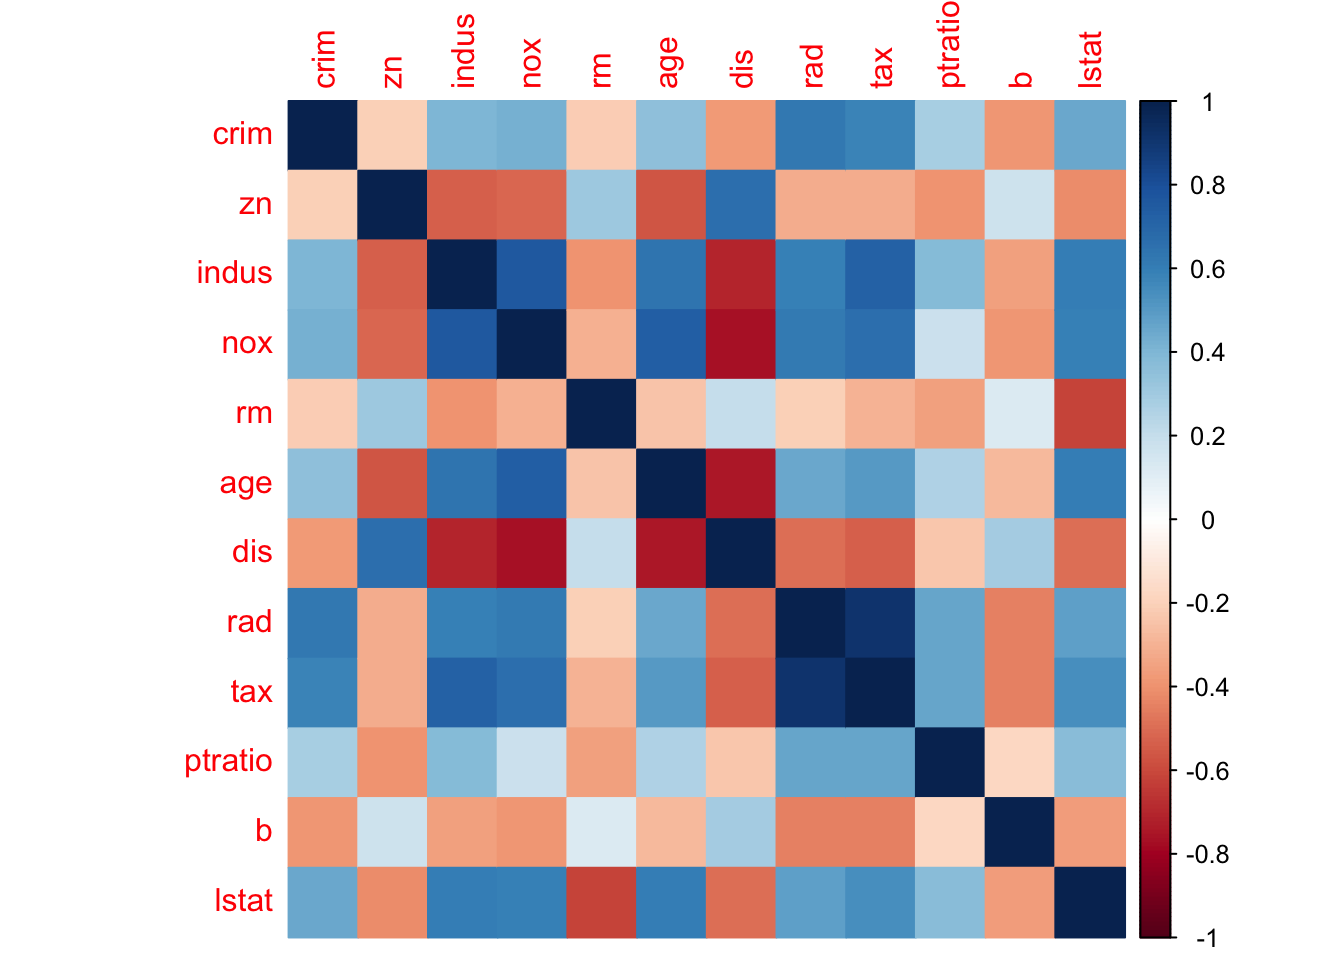
\includegraphics{_main_files/figure-latex/unnamed-chunk-151-1.pdf}

Now it's time to check the distribution of the features. For this I want to make a boxplot, but for that I need to reshape the dataset first. As seen in Chapter 1, \texttt{tidyr::pivot\_longer()} can be used to convert the data into long format.

\begin{Shaded}
\begin{Highlighting}[]
\NormalTok{dfm }\OtherTok{\textless{}{-}}\NormalTok{ df }\SpecialCharTok{\%\textgreater{}\%} \FunctionTok{select}\NormalTok{(}\SpecialCharTok{{-}}\FunctionTok{c}\NormalTok{(medv, chas)) }\SpecialCharTok{\%\textgreater{}\%}
  \FunctionTok{pivot\_longer}\NormalTok{(}\FunctionTok{everything}\NormalTok{(), }\AttributeTok{names\_to =} \StringTok{\textquotesingle{}Feature\textquotesingle{}}\NormalTok{, }\AttributeTok{values\_to =} \StringTok{\textquotesingle{}Value\textquotesingle{}}\NormalTok{)}

\NormalTok{dfm}
\end{Highlighting}
\end{Shaded}

\begin{verbatim}
## # A tibble: 6,072 x 2
##    Feature     Value
##    <chr>       <dbl>
##  1 crim      0.00632
##  2 zn       18      
##  3 indus     2.31   
##  4 nox       0.538  
##  5 rm        6.58   
##  6 age      65.2    
##  7 dis       4.09   
##  8 rad       1      
##  9 tax     296      
## 10 ptratio  15.3    
## # ... with 6,062 more rows
\end{verbatim}

Now it's trivial to use \texttt{ggplot()} to make the boxplot:

\begin{Shaded}
\begin{Highlighting}[]
\FunctionTok{ggplot}\NormalTok{(dfm, }\FunctionTok{aes}\NormalTok{(}\AttributeTok{x =}\NormalTok{ Feature, }\AttributeTok{y =}\NormalTok{ Value)) }\SpecialCharTok{+} 
  \FunctionTok{geom\_boxplot}\NormalTok{(}\FunctionTok{aes}\NormalTok{(}\AttributeTok{fill =}\NormalTok{ Feature), }\AttributeTok{alpha =}\NormalTok{ .}\DecValTok{6}\NormalTok{) }\SpecialCharTok{+} 
  \FunctionTok{theme\_bw}\NormalTok{() }\SpecialCharTok{+} \FunctionTok{theme}\NormalTok{(}\AttributeTok{legend.position =} \StringTok{\textquotesingle{}none\textquotesingle{}}\NormalTok{)}
\end{Highlighting}
\end{Shaded}

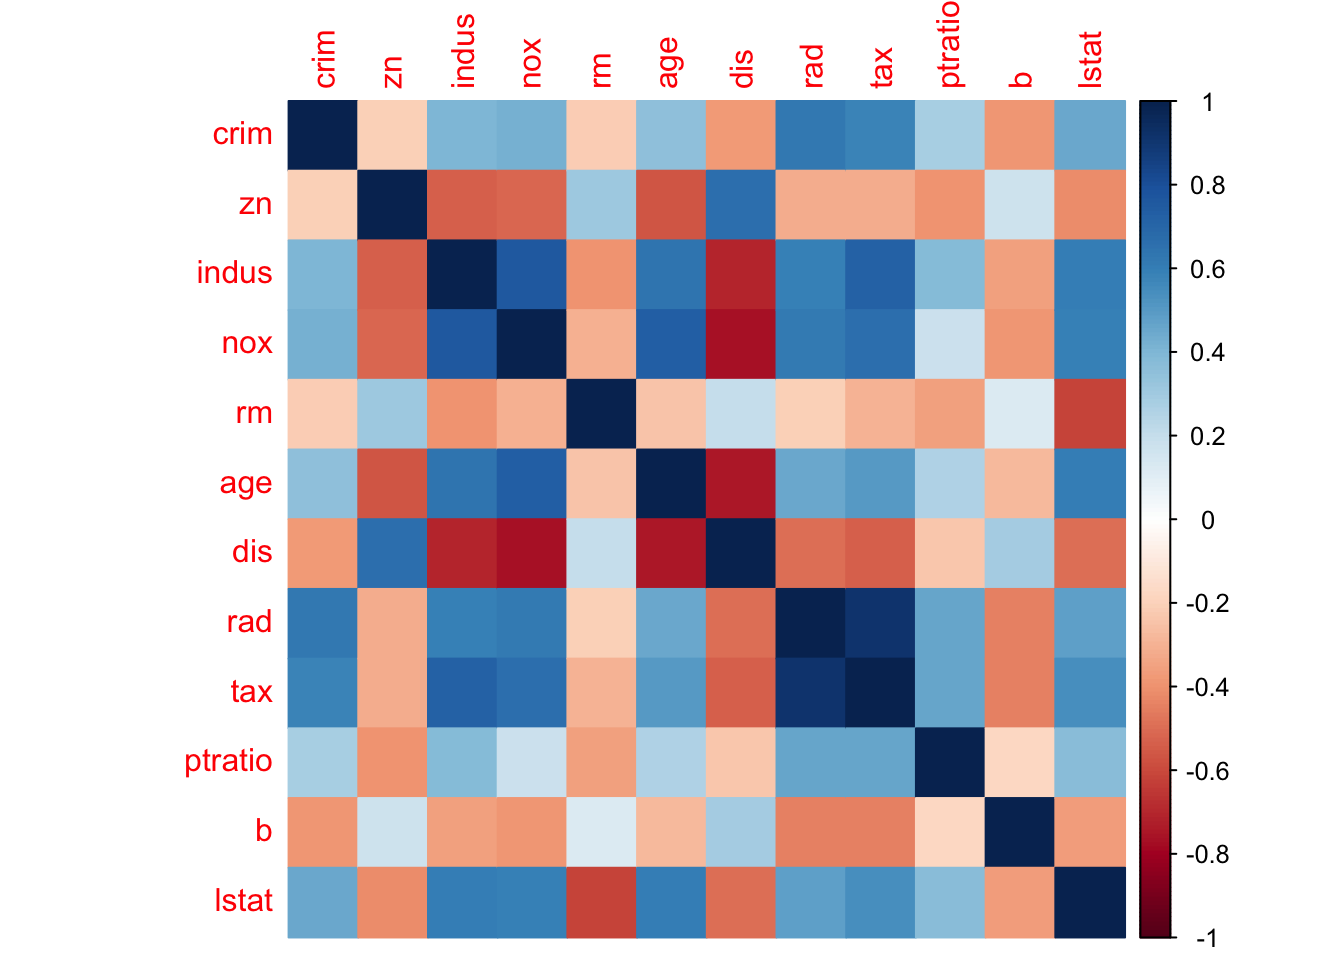
\includegraphics{_main_files/figure-latex/unnamed-chunk-153-1.pdf}

It looks like the scales for the features are not consistent. This is common in real-life data and for most ML algorithms, features need to be preprocessed. I will cover this in the future chapters, but in brief, we can calculate the z-score as such for each predictor:

\begin{Shaded}
\begin{Highlighting}[]
\NormalTok{zs }\OtherTok{\textless{}{-}} \ControlFlowTok{function}\NormalTok{(x)\{}
\NormalTok{  (x }\SpecialCharTok{{-}} \FunctionTok{mean}\NormalTok{(x)) }\SpecialCharTok{/} \FunctionTok{sd}\NormalTok{(x)}
\NormalTok{\}}

\NormalTok{df\_s }\OtherTok{\textless{}{-}}\NormalTok{ df }\SpecialCharTok{\%\textgreater{}\%} \FunctionTok{select}\NormalTok{(}\SpecialCharTok{{-}}\FunctionTok{c}\NormalTok{(medv, chas)) }\SpecialCharTok{\%\textgreater{}\%}
  \FunctionTok{mutate}\NormalTok{(}\FunctionTok{across}\NormalTok{(}\FunctionTok{everything}\NormalTok{(), zs))}

\NormalTok{df\_s}
\end{Highlighting}
\end{Shaded}

\begin{verbatim}
## # A tibble: 506 x 12
##      crim      zn  indus    nox     rm     age   dis    rad
##     <dbl>   <dbl>  <dbl>  <dbl>  <dbl>   <dbl> <dbl>  <dbl>
##  1 -0.419  0.285  -1.29  -0.144  0.413 -0.120  0.140 -0.982
##  2 -0.417 -0.487  -0.593 -0.740  0.194  0.367  0.557 -0.867
##  3 -0.417 -0.487  -0.593 -0.740  1.28  -0.266  0.557 -0.867
##  4 -0.416 -0.487  -1.31  -0.834  1.02  -0.809  1.08  -0.752
##  5 -0.412 -0.487  -1.31  -0.834  1.23  -0.511  1.08  -0.752
##  6 -0.417 -0.487  -1.31  -0.834  0.207 -0.351  1.08  -0.752
##  7 -0.410  0.0487 -0.476 -0.265 -0.388 -0.0702 0.838 -0.522
##  8 -0.403  0.0487 -0.476 -0.265 -0.160  0.978  1.02  -0.522
##  9 -0.396  0.0487 -0.476 -0.265 -0.930  1.12   1.09  -0.522
## 10 -0.400  0.0487 -0.476 -0.265 -0.399  0.615  1.33  -0.522
## # ... with 496 more rows, and 4 more variables: tax <dbl>,
## #   ptratio <dbl>, b <dbl>, lstat <dbl>
\end{verbatim}

Now the boxplots look more uniform:

\begin{Shaded}
\begin{Highlighting}[]
\NormalTok{df\_sm }\OtherTok{\textless{}{-}}\NormalTok{ df\_s }\SpecialCharTok{\%\textgreater{}\%} \FunctionTok{pivot\_longer}\NormalTok{(}\FunctionTok{everything}\NormalTok{(), }
                               \AttributeTok{names\_to =} \StringTok{\textquotesingle{}Feature\textquotesingle{}}\NormalTok{, }
                               \AttributeTok{values\_to =} \StringTok{\textquotesingle{}Value\textquotesingle{}}\NormalTok{)}

\FunctionTok{ggplot}\NormalTok{(df\_sm, }\FunctionTok{aes}\NormalTok{(}\AttributeTok{x =}\NormalTok{ Feature, }\AttributeTok{y =}\NormalTok{ Value)) }\SpecialCharTok{+} 
  \FunctionTok{geom\_boxplot}\NormalTok{(}\FunctionTok{aes}\NormalTok{(}\AttributeTok{fill =}\NormalTok{ Feature), }\AttributeTok{alpha =}\NormalTok{ .}\DecValTok{6}\NormalTok{) }\SpecialCharTok{+} 
  \FunctionTok{theme\_bw}\NormalTok{() }\SpecialCharTok{+} \FunctionTok{theme}\NormalTok{(}\AttributeTok{legend.position =} \StringTok{\textquotesingle{}none\textquotesingle{}}\NormalTok{)}
\end{Highlighting}
\end{Shaded}

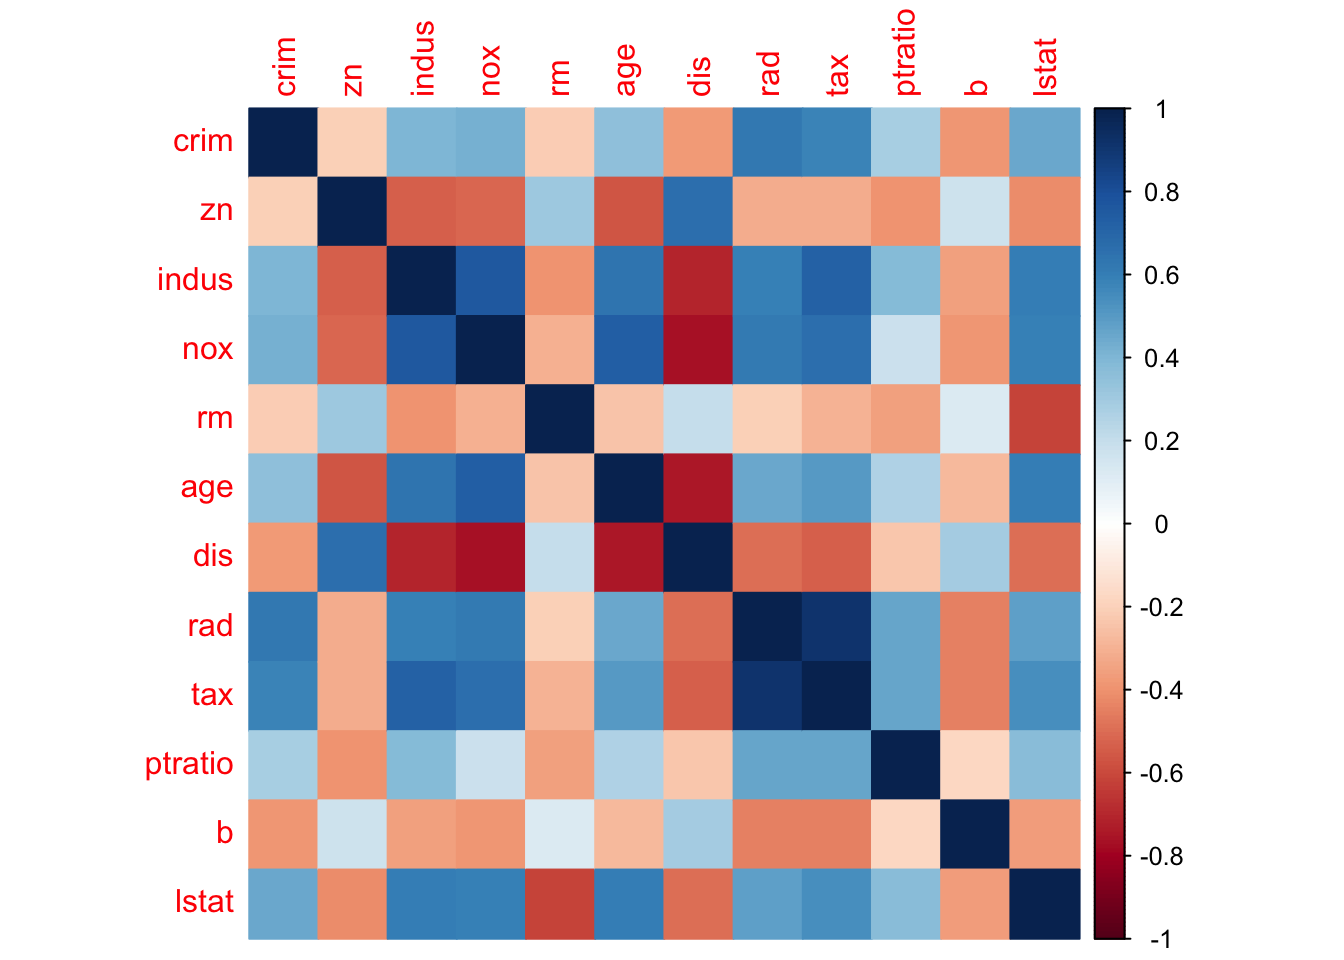
\includegraphics{_main_files/figure-latex/unnamed-chunk-155-1.pdf}

How about our target variable - the housing price? This column is also continuous so let's check the shape of this distribution using a histogram:

\begin{Shaded}
\begin{Highlighting}[]
\FunctionTok{hist}\NormalTok{(df}\SpecialCharTok{$}\NormalTok{medv)}
\end{Highlighting}
\end{Shaded}

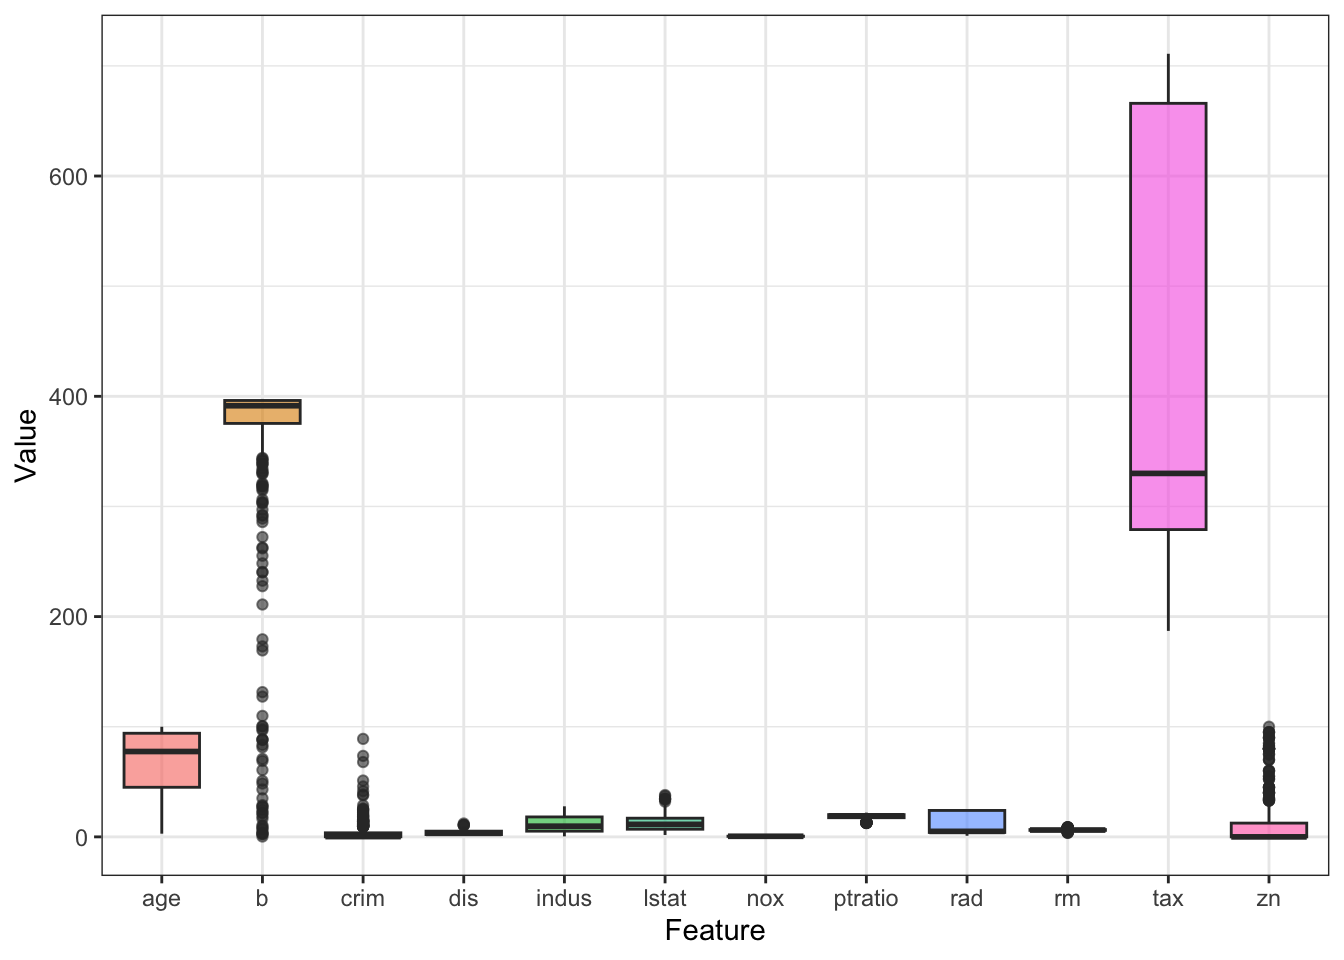
\includegraphics{_main_files/figure-latex/unnamed-chunk-156-1.pdf}

It looks like the mean value for \texttt{medv} is at around 22 to 23. Changing the number of bins can give us a better look, if needed.

Since the target variable is continuous, we can easily fit a simple linear model to check for relationships between the predictors and the target. This part may be delving a bit deeper than our initial goal of EDA, but it's still useful to make us aware of possible relationships in our data.

\begin{Shaded}
\begin{Highlighting}[]
\NormalTok{df\_num }\OtherTok{\textless{}{-}}\NormalTok{ df }\SpecialCharTok{\%\textgreater{}\%} \FunctionTok{select}\NormalTok{(}\SpecialCharTok{{-}}\NormalTok{chas)}

\NormalTok{lm\_mod }\OtherTok{\textless{}{-}} \FunctionTok{lm}\NormalTok{(medv }\SpecialCharTok{\textasciitilde{}}\NormalTok{ ., }\AttributeTok{data =}\NormalTok{ df\_num)}
\FunctionTok{summary}\NormalTok{(lm\_mod)}
\end{Highlighting}
\end{Shaded}

\begin{verbatim}
## 
## Call:
## lm(formula = medv ~ ., data = df_num)
## 
## Residuals:
##      Min       1Q   Median       3Q      Max 
## -13.3968  -2.8103  -0.6455   1.9141  26.3755 
## 
## Coefficients:
##               Estimate Std. Error t value Pr(>|t|)    
## (Intercept)  36.891960   5.146516   7.168 2.79e-12 ***
## crim         -0.113139   0.033113  -3.417 0.000686 ***
## zn            0.047052   0.013847   3.398 0.000734 ***
## indus         0.040311   0.061707   0.653 0.513889    
## nox         -17.366999   3.851224  -4.509 8.13e-06 ***
## rm            3.850492   0.421402   9.137  < 2e-16 ***
## age           0.002784   0.013309   0.209 0.834407    
## dis          -1.485374   0.201187  -7.383 6.64e-13 ***
## rad           0.328311   0.066542   4.934 1.10e-06 ***
## tax          -0.013756   0.003766  -3.653 0.000287 ***
## ptratio      -0.990958   0.131399  -7.542 2.25e-13 ***
## b             0.009741   0.002706   3.600 0.000351 ***
## lstat        -0.534158   0.051072 -10.459  < 2e-16 ***
## ---
## Signif. codes:  
## 0 '***' 0.001 '**' 0.01 '*' 0.05 '.' 0.1 ' ' 1
## 
## Residual standard error: 4.787 on 493 degrees of freedom
## Multiple R-squared:  0.7355, Adjusted R-squared:  0.7291 
## F-statistic: 114.3 on 12 and 493 DF,  p-value: < 2.2e-16
\end{verbatim}

An ANOVA table on the fitted model gives us additional info such as the mean sum of squares:

\begin{Shaded}
\begin{Highlighting}[]
\FunctionTok{anova}\NormalTok{(lm\_mod)}
\end{Highlighting}
\end{Shaded}

\begin{verbatim}
## Analysis of Variance Table
## 
## Response: medv
##            Df  Sum Sq Mean Sq  F value    Pr(>F)    
## crim        1  6440.8  6440.8 281.0564 < 2.2e-16 ***
## zn          1  3554.3  3554.3 155.1005 < 2.2e-16 ***
## indus       1  2551.2  2551.2 111.3283 < 2.2e-16 ***
## nox         1    28.7    28.7   1.2507   0.26397    
## rm          1 11794.6 11794.6 514.6823 < 2.2e-16 ***
## age         1    74.1    74.1   3.2330   0.07278 .  
## dis         1  1858.3  1858.3  81.0890 < 2.2e-16 ***
## rad         1    46.9    46.9   2.0447   0.15337    
## tax         1   454.1   454.1  19.8158 1.055e-05 ***
## ptratio     1  1458.7  1458.7  63.6538 1.046e-14 ***
## b           1   650.0   650.0  28.3656 1.529e-07 ***
## lstat       1  2506.8  2506.8 109.3905 < 2.2e-16 ***
## Residuals 493 11297.8    22.9                       
## ---
## Signif. codes:  
## 0 '***' 0.001 '**' 0.01 '*' 0.05 '.' 0.1 ' ' 1
\end{verbatim}

The \texttt{broom} package is useful in converting summaries of model objects into workable tibbles:

\begin{Shaded}
\begin{Highlighting}[]
\FunctionTok{library}\NormalTok{(broom)}
\FunctionTok{tidy}\NormalTok{(lm\_mod)}
\end{Highlighting}
\end{Shaded}

\begin{verbatim}
## # A tibble: 13 x 5
##    term         estimate std.error statistic  p.value
##    <chr>           <dbl>     <dbl>     <dbl>    <dbl>
##  1 (Intercept)  36.9       5.15        7.17  2.79e-12
##  2 crim         -0.113     0.0331     -3.42  6.86e- 4
##  3 zn            0.0471    0.0138      3.40  7.34e- 4
##  4 indus         0.0403    0.0617      0.653 5.14e- 1
##  5 nox         -17.4       3.85       -4.51  8.13e- 6
##  6 rm            3.85      0.421       9.14  1.66e-18
##  7 age           0.00278   0.0133      0.209 8.34e- 1
##  8 dis          -1.49      0.201      -7.38  6.64e-13
##  9 rad           0.328     0.0665      4.93  1.10e- 6
## 10 tax          -0.0138    0.00377    -3.65  2.87e- 4
## 11 ptratio      -0.991     0.131      -7.54  2.25e-13
## 12 b             0.00974   0.00271     3.60  3.51e- 4
## 13 lstat        -0.534     0.0511    -10.5   2.94e-23
\end{verbatim}

Since we seem to have linear relationships across our dataset, we can use scatterplots in combination with correlation analysis to generate useful visualizations:

\begin{Shaded}
\begin{Highlighting}[]
\FunctionTok{library}\NormalTok{(ggpubr)}
\FunctionTok{ggplot}\NormalTok{(df\_num, }\FunctionTok{aes}\NormalTok{(}\AttributeTok{x =}\NormalTok{ rm, }\AttributeTok{y =}\NormalTok{ medv)) }\SpecialCharTok{+} 
  \FunctionTok{geom\_point}\NormalTok{() }\SpecialCharTok{+} 
  \FunctionTok{geom\_smooth}\NormalTok{(}\AttributeTok{method =} \StringTok{\textquotesingle{}lm\textquotesingle{}}\NormalTok{) }\SpecialCharTok{+} \FunctionTok{theme\_bw}\NormalTok{() }\SpecialCharTok{+} 
  \FunctionTok{stat\_cor}\NormalTok{(}\AttributeTok{method =} \StringTok{\textquotesingle{}pearson\textquotesingle{}}\NormalTok{)}
\end{Highlighting}
\end{Shaded}

\begin{verbatim}
## `geom_smooth()` using formula = 'y ~ x'
\end{verbatim}

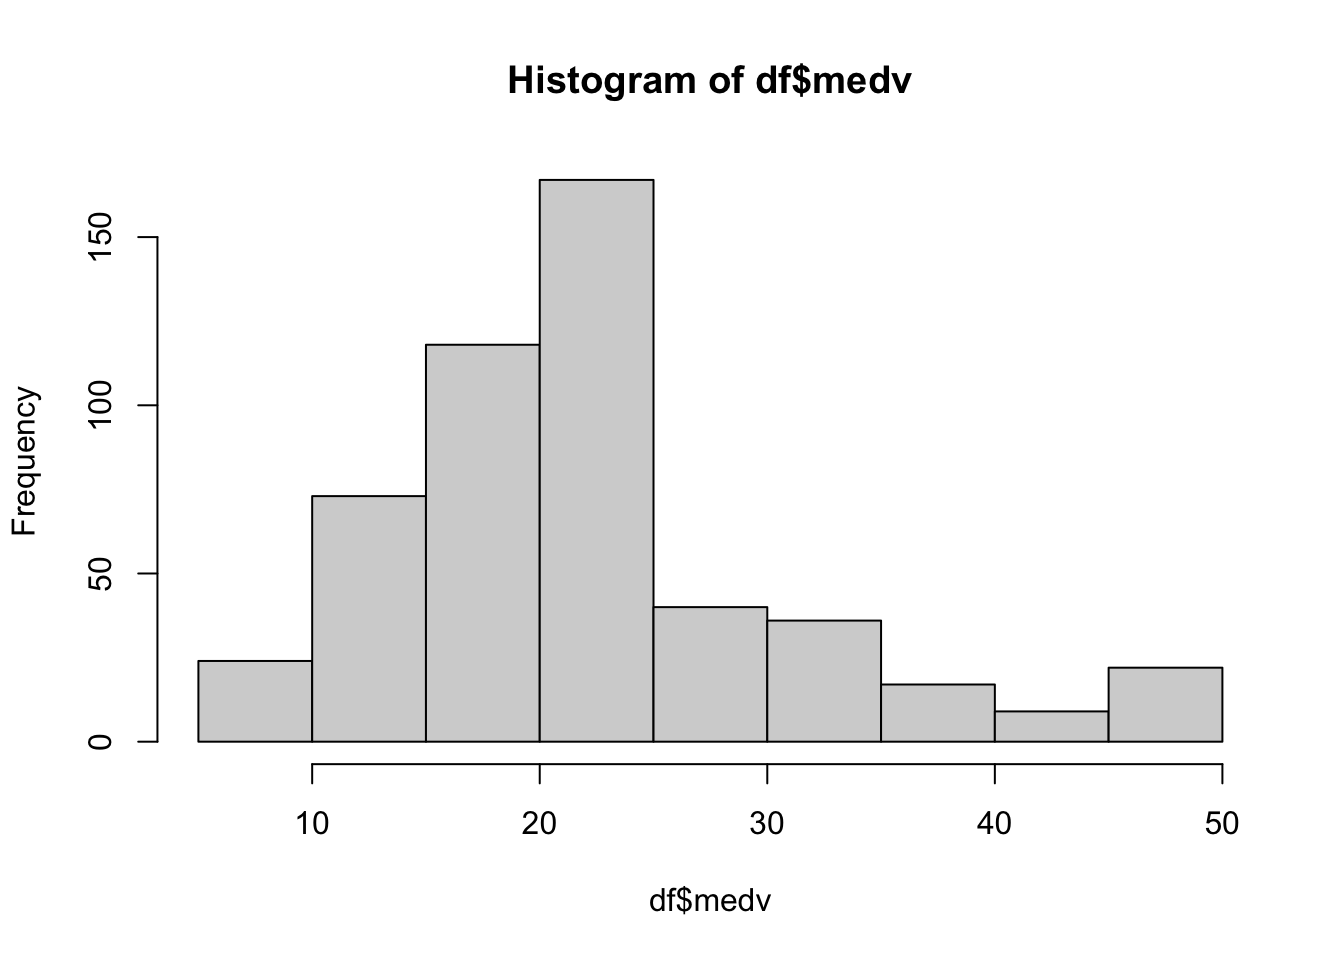
\includegraphics{_main_files/figure-latex/unnamed-chunk-160-1.pdf}

Oops! Even though it's clear there is indeed a linear relationship between the number of rooms \texttt{rm} and the housing price \texttt{medv}, it looks like there is a strange behaviour at \texttt{medv\ ==\ 50}. Indeed, it looks like the measurement was artificially capped at 50 and there are 16 instances where this value is found:

\begin{Shaded}
\begin{Highlighting}[]
\FunctionTok{length}\NormalTok{(df}\SpecialCharTok{$}\NormalTok{medv[df}\SpecialCharTok{$}\NormalTok{medv }\SpecialCharTok{==} \DecValTok{50}\NormalTok{])}
\end{Highlighting}
\end{Shaded}

\begin{verbatim}
## [1] 16
\end{verbatim}

Since we're only concerned with EDA for now, we won't delve further into how we're going to tackle this. Of course, if we are training a prediction model, we probably shouldn't leave the values capped like that as is. EDA have made us aware of this before we started high-level modeling tasks, and that's good.

Let's circle back to the dummy variable \texttt{chas}. Since this is a factor, let's treat them as groups and compare the distribution of \texttt{medv} using a Wilcoxon test:

\begin{Shaded}
\begin{Highlighting}[]
\NormalTok{df\_chas }\OtherTok{\textless{}{-}}\NormalTok{ df }\SpecialCharTok{\%\textgreater{}\%} \FunctionTok{select}\NormalTok{(medv, chas)}

\FunctionTok{ggplot}\NormalTok{(df\_chas, }\FunctionTok{aes}\NormalTok{(}\AttributeTok{x =}\NormalTok{ chas, }\AttributeTok{y =}\NormalTok{ medv)) }\SpecialCharTok{+}
  \FunctionTok{geom\_boxplot}\NormalTok{(}\FunctionTok{aes}\NormalTok{(}\AttributeTok{fill =}\NormalTok{ chas), }\AttributeTok{alpha =}\NormalTok{ .}\DecValTok{6}\NormalTok{) }\SpecialCharTok{+} 
  \FunctionTok{theme\_bw}\NormalTok{() }\SpecialCharTok{+} \FunctionTok{theme}\NormalTok{(}\AttributeTok{legend.position =} \StringTok{\textquotesingle{}none\textquotesingle{}}\NormalTok{) }\SpecialCharTok{+}
  \FunctionTok{stat\_compare\_means}\NormalTok{(}\AttributeTok{method =} \StringTok{\textquotesingle{}wilcox\textquotesingle{}}\NormalTok{)}
\end{Highlighting}
\end{Shaded}

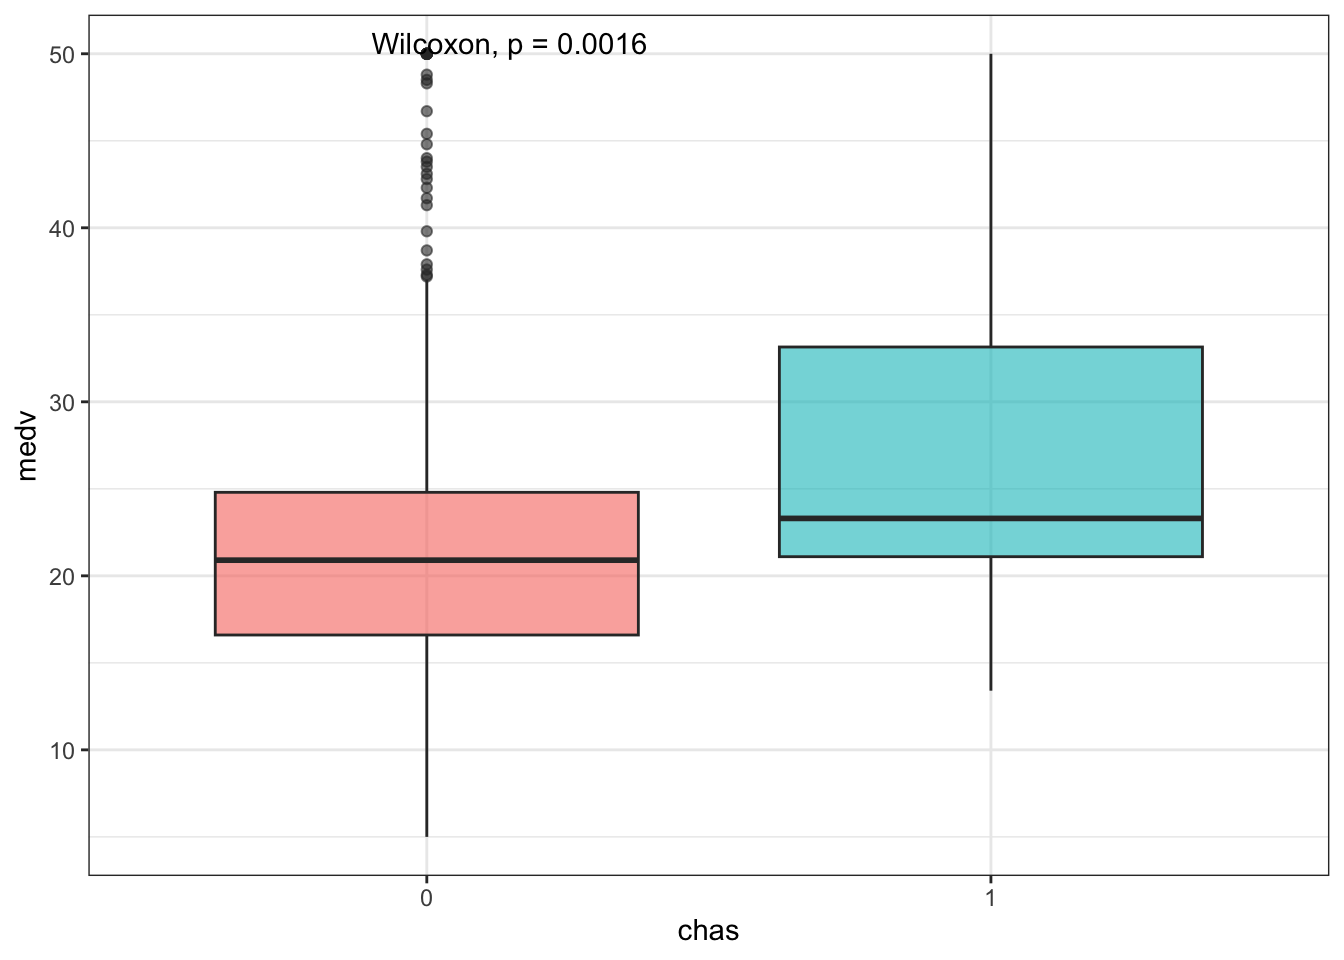
\includegraphics{_main_files/figure-latex/unnamed-chunk-162-1.pdf}

Boxplots are nice but violin plots give us a further look at the shape of the distributions: this way we can actually see that \texttt{medv} values are capped at 50.

\begin{Shaded}
\begin{Highlighting}[]
\FunctionTok{ggplot}\NormalTok{(df\_chas, }\FunctionTok{aes}\NormalTok{(}\AttributeTok{x =}\NormalTok{ chas, }\AttributeTok{y =}\NormalTok{ medv)) }\SpecialCharTok{+}
  \FunctionTok{geom\_violin}\NormalTok{(}\FunctionTok{aes}\NormalTok{(}\AttributeTok{fill =}\NormalTok{ chas), }\AttributeTok{alpha =}\NormalTok{ .}\DecValTok{6}\NormalTok{) }\SpecialCharTok{+} 
  \FunctionTok{theme\_bw}\NormalTok{() }\SpecialCharTok{+} \FunctionTok{theme}\NormalTok{(}\AttributeTok{legend.position =} \StringTok{\textquotesingle{}none\textquotesingle{}}\NormalTok{) }\SpecialCharTok{+}
  \FunctionTok{stat\_compare\_means}\NormalTok{(}\AttributeTok{method =} \StringTok{\textquotesingle{}wilcox\textquotesingle{}}\NormalTok{)}
\end{Highlighting}
\end{Shaded}

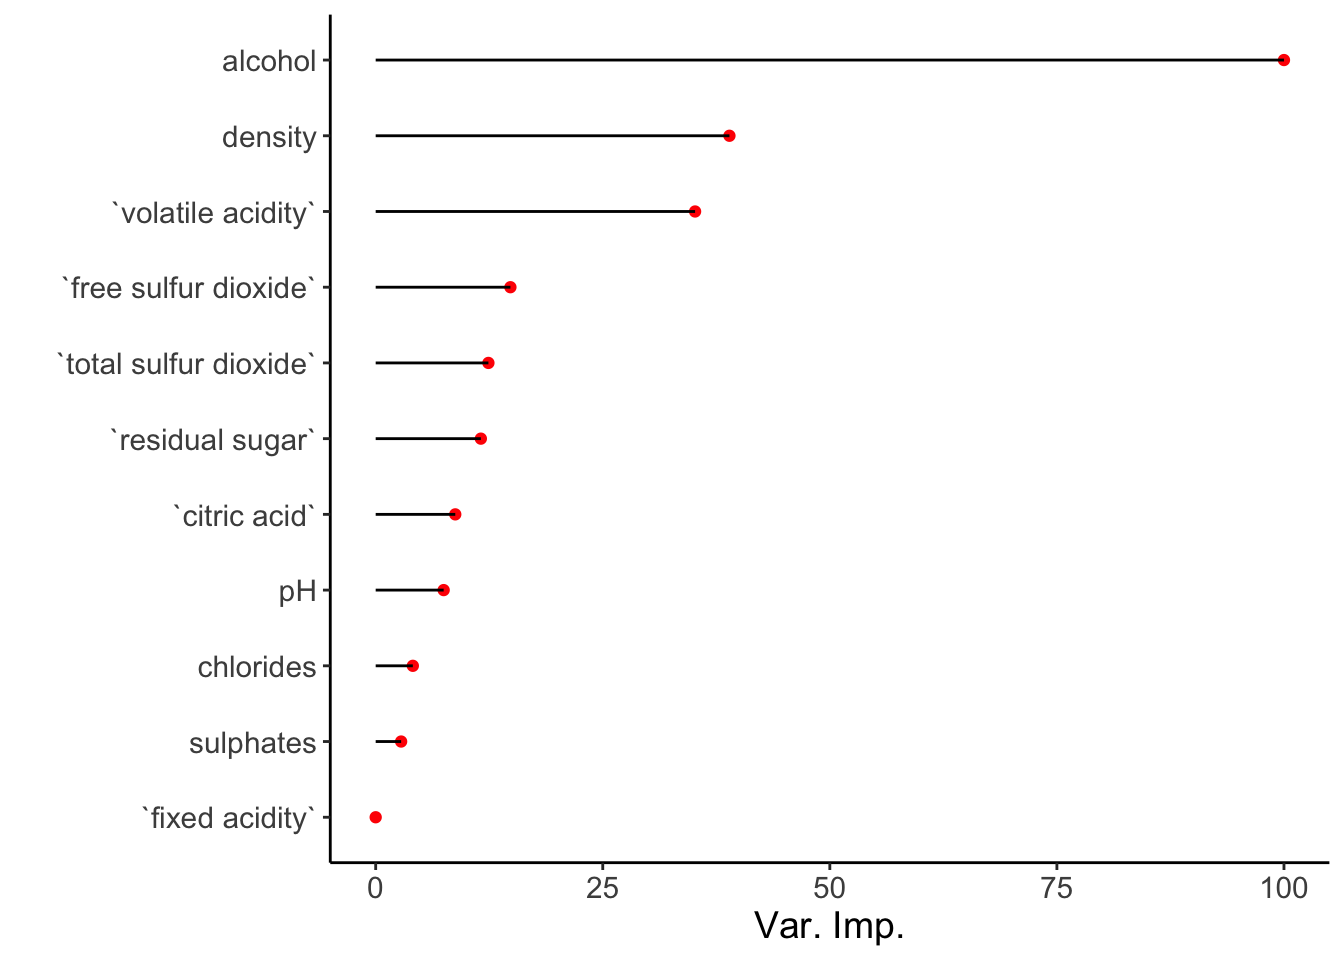
\includegraphics{_main_files/figure-latex/unnamed-chunk-163-1.pdf}

\hypertarget{workflow-2-dates-and-ordinal-data}{%
\section{Workflow 2: dates and ordinal data}\label{workflow-2-dates-and-ordinal-data}}

For this part I will pull the \texttt{Ozone} data from \texttt{mlbench} which has the following three columns as the first three: integers coding for the month, integers coding for the day of the month, and integers coding for the day of the week, with Monday coded as the first day (i.e., 1 = Mon., 2 = Tues.,\ldots). The rest of the columns correspond to various weather measurements as continuous values such as the temperature, humidity, and visibility.

\begin{Shaded}
\begin{Highlighting}[]
\FunctionTok{data}\NormalTok{(}\StringTok{\textquotesingle{}Ozone\textquotesingle{}}\NormalTok{)}
\NormalTok{df }\OtherTok{\textless{}{-}} \FunctionTok{as\_tibble}\NormalTok{(Ozone)}
\NormalTok{df}
\end{Highlighting}
\end{Shaded}

\begin{verbatim}
## # A tibble: 366 x 13
##    V1    V2    V3       V4    V5    V6    V7    V8    V9
##    <fct> <fct> <fct> <dbl> <dbl> <dbl> <dbl> <dbl> <dbl>
##  1 1     1     4         3  5480     8    20    NA  NA  
##  2 1     2     5         3  5660     6    NA    38  NA  
##  3 1     3     6         3  5710     4    28    40  NA  
##  4 1     4     7         5  5700     3    37    45  NA  
##  5 1     5     1         5  5760     3    51    54  45.3
##  6 1     6     2         6  5720     4    69    35  49.6
##  7 1     7     3         4  5790     6    19    45  46.4
##  8 1     8     4         4  5790     3    25    55  52.7
##  9 1     9     5         6  5700     3    73    41  48.0
## 10 1     10    6         7  5700     3    59    44  NA  
## # ... with 356 more rows, and 4 more variables: V10 <dbl>,
## #   V11 <dbl>, V12 <dbl>, V13 <dbl>
\end{verbatim}

It's not necessary in this case, but since we are working with dates let's make the date labels easier to read. Using \texttt{lubridate} I will convert the month labels into a factor with character levels. Then using base R's \texttt{weekdays()} I will convert the days of the week to characters as well.

\begin{Shaded}
\begin{Highlighting}[]
\FunctionTok{library}\NormalTok{(lubridate)}
\end{Highlighting}
\end{Shaded}

\begin{verbatim}
## 
## Attaching package: 'lubridate'
\end{verbatim}

\begin{verbatim}
## The following objects are masked from 'package:data.table':
## 
##     hour, isoweek, mday, minute, month, quarter,
##     second, wday, week, yday, year
\end{verbatim}

\begin{verbatim}
## The following objects are masked from 'package:base':
## 
##     date, intersect, setdiff, union
\end{verbatim}

\begin{Shaded}
\begin{Highlighting}[]
\NormalTok{df }\OtherTok{\textless{}{-}}\NormalTok{ df }\SpecialCharTok{\%\textgreater{}\%} 
  \FunctionTok{mutate}\NormalTok{(}\AttributeTok{V1 =}\NormalTok{ lubridate}\SpecialCharTok{::}\FunctionTok{month}\NormalTok{(}\FunctionTok{as.numeric}\NormalTok{(V1), }
                               \AttributeTok{label =} \ConstantTok{TRUE}\NormalTok{)) }\SpecialCharTok{\%\textgreater{}\%}
  \FunctionTok{mutate}\NormalTok{(}\AttributeTok{V3 =} \FunctionTok{weekdays}\NormalTok{(}\FunctionTok{.Date}\NormalTok{(}\DecValTok{4}\SpecialCharTok{:}\DecValTok{10}\NormalTok{))[df}\SpecialCharTok{$}\NormalTok{V3])}

\NormalTok{df}
\end{Highlighting}
\end{Shaded}

\begin{verbatim}
## # A tibble: 366 x 13
##    V1    V2    V3           V4    V5    V6    V7    V8    V9
##    <ord> <fct> <chr>     <dbl> <dbl> <dbl> <dbl> <dbl> <dbl>
##  1 Jan   1     Thursday      3  5480     8    20    NA  NA  
##  2 Jan   2     Friday        3  5660     6    NA    38  NA  
##  3 Jan   3     Saturday      3  5710     4    28    40  NA  
##  4 Jan   4     Sunday        5  5700     3    37    45  NA  
##  5 Jan   5     Monday        5  5760     3    51    54  45.3
##  6 Jan   6     Tuesday       6  5720     4    69    35  49.6
##  7 Jan   7     Wednesday     4  5790     6    19    45  46.4
##  8 Jan   8     Thursday      4  5790     3    25    55  52.7
##  9 Jan   9     Friday        6  5700     3    73    41  48.0
## 10 Jan   10    Saturday      7  5700     3    59    44  NA  
## # ... with 356 more rows, and 4 more variables: V10 <dbl>,
## #   V11 <dbl>, V12 <dbl>, V13 <dbl>
\end{verbatim}

\begin{Shaded}
\begin{Highlighting}[]
\NormalTok{df }\OtherTok{\textless{}{-}}\NormalTok{ df }\SpecialCharTok{\%\textgreater{}\%} 
  \FunctionTok{mutate}\NormalTok{(}\AttributeTok{V3 =} \FunctionTok{factor}\NormalTok{(V3, }\AttributeTok{levels=} 
                       \FunctionTok{weekdays}\NormalTok{(}\FunctionTok{.Date}\NormalTok{(}\DecValTok{4}\SpecialCharTok{:}\DecValTok{10}\NormalTok{))))}
\end{Highlighting}
\end{Shaded}

Another thing to note - since this data is temporal data, there's a big chance there are many missing values due to external factors. Let's see:

\begin{Shaded}
\begin{Highlighting}[]
\FunctionTok{vapply}\NormalTok{(df, }\ControlFlowTok{function}\NormalTok{(x) }\FunctionTok{sum}\NormalTok{(}\FunctionTok{is.na}\NormalTok{(x)), }\FunctionTok{double}\NormalTok{(}\DecValTok{1}\NormalTok{))}
\end{Highlighting}
\end{Shaded}

\begin{verbatim}
##  V1  V2  V3  V4  V5  V6  V7  V8  V9 V10 V11 V12 V13 
##   0   0   0   5  12   0  15   2 139  15   1  14   0
\end{verbatim}

Column \texttt{V9}, which correspond to temperature measured in El Monte, CA has 139 missing values! Immediately you could argue we can replace these with 0s but remember the nature of this data - a 0 degree weather has actual meaning. Imputation cases like this are tricky and that will be important during modeling tasks.

Since we are working with ordinal data - in our case, data points over time, it makes sense to make a trendline. Using \texttt{facet\_wrap()}, in \texttt{ggplot()}, I can make a grid based on the time of the month; here I am plotting \texttt{V8} - temperature measured at Sandburg, CA - versus \texttt{V2} - day of the month.

\begin{Shaded}
\begin{Highlighting}[]
\FunctionTok{ggplot}\NormalTok{(df, }\FunctionTok{aes}\NormalTok{(}\AttributeTok{x =}\NormalTok{ V2, }\AttributeTok{y =}\NormalTok{ V8)) }\SpecialCharTok{+} 
  \FunctionTok{geom\_point}\NormalTok{() }\SpecialCharTok{+} \FunctionTok{geom\_line}\NormalTok{(}\FunctionTok{aes}\NormalTok{(}\AttributeTok{group =} \DecValTok{1}\NormalTok{)) }\SpecialCharTok{+}
  \FunctionTok{facet\_wrap}\NormalTok{(}\SpecialCharTok{\textasciitilde{}}\NormalTok{ V1) }\SpecialCharTok{+} \FunctionTok{theme\_bw}\NormalTok{() }\SpecialCharTok{+}
  \FunctionTok{theme}\NormalTok{(}\AttributeTok{axis.text.x =} \FunctionTok{element\_blank}\NormalTok{())}
\end{Highlighting}
\end{Shaded}

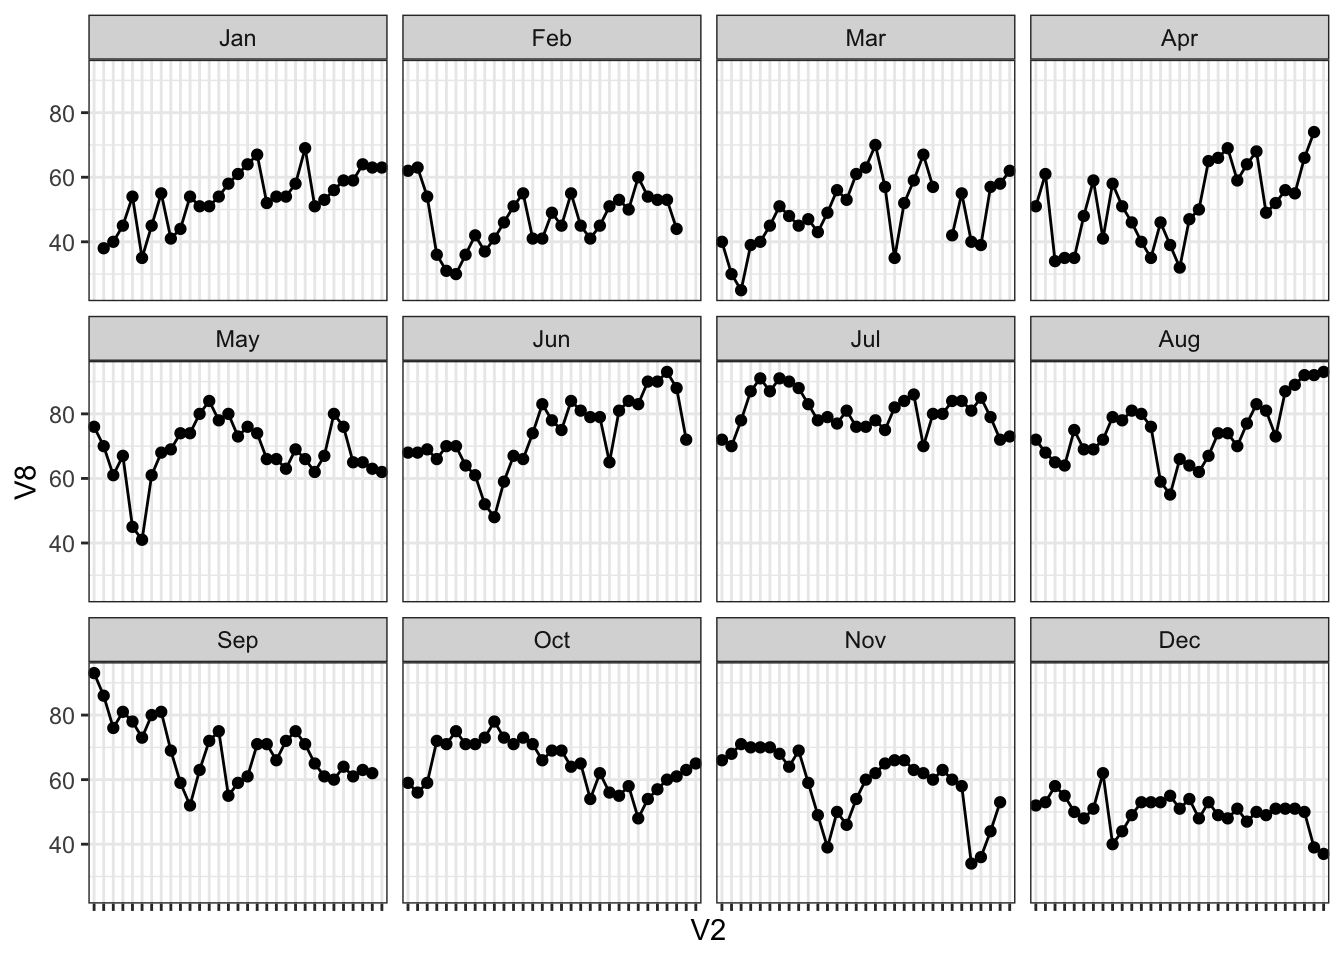
\includegraphics{_main_files/figure-latex/unnamed-chunk-168-1.pdf}

For a visual reference, let's see what happens when we plot the temperature at El Monte instead, with all those missing values:

\begin{Shaded}
\begin{Highlighting}[]
\FunctionTok{ggplot}\NormalTok{(df, }\FunctionTok{aes}\NormalTok{(}\AttributeTok{x =}\NormalTok{ V2, }\AttributeTok{y =}\NormalTok{ V9)) }\SpecialCharTok{+} 
  \FunctionTok{geom\_point}\NormalTok{() }\SpecialCharTok{+} \FunctionTok{geom\_line}\NormalTok{(}\FunctionTok{aes}\NormalTok{(}\AttributeTok{group =} \DecValTok{1}\NormalTok{)) }\SpecialCharTok{+}
  \FunctionTok{facet\_wrap}\NormalTok{(}\SpecialCharTok{\textasciitilde{}}\NormalTok{ V1) }\SpecialCharTok{+} \FunctionTok{theme\_bw}\NormalTok{() }\SpecialCharTok{+}
  \FunctionTok{theme}\NormalTok{(}\AttributeTok{axis.text.x =} \FunctionTok{element\_blank}\NormalTok{())}
\end{Highlighting}
\end{Shaded}

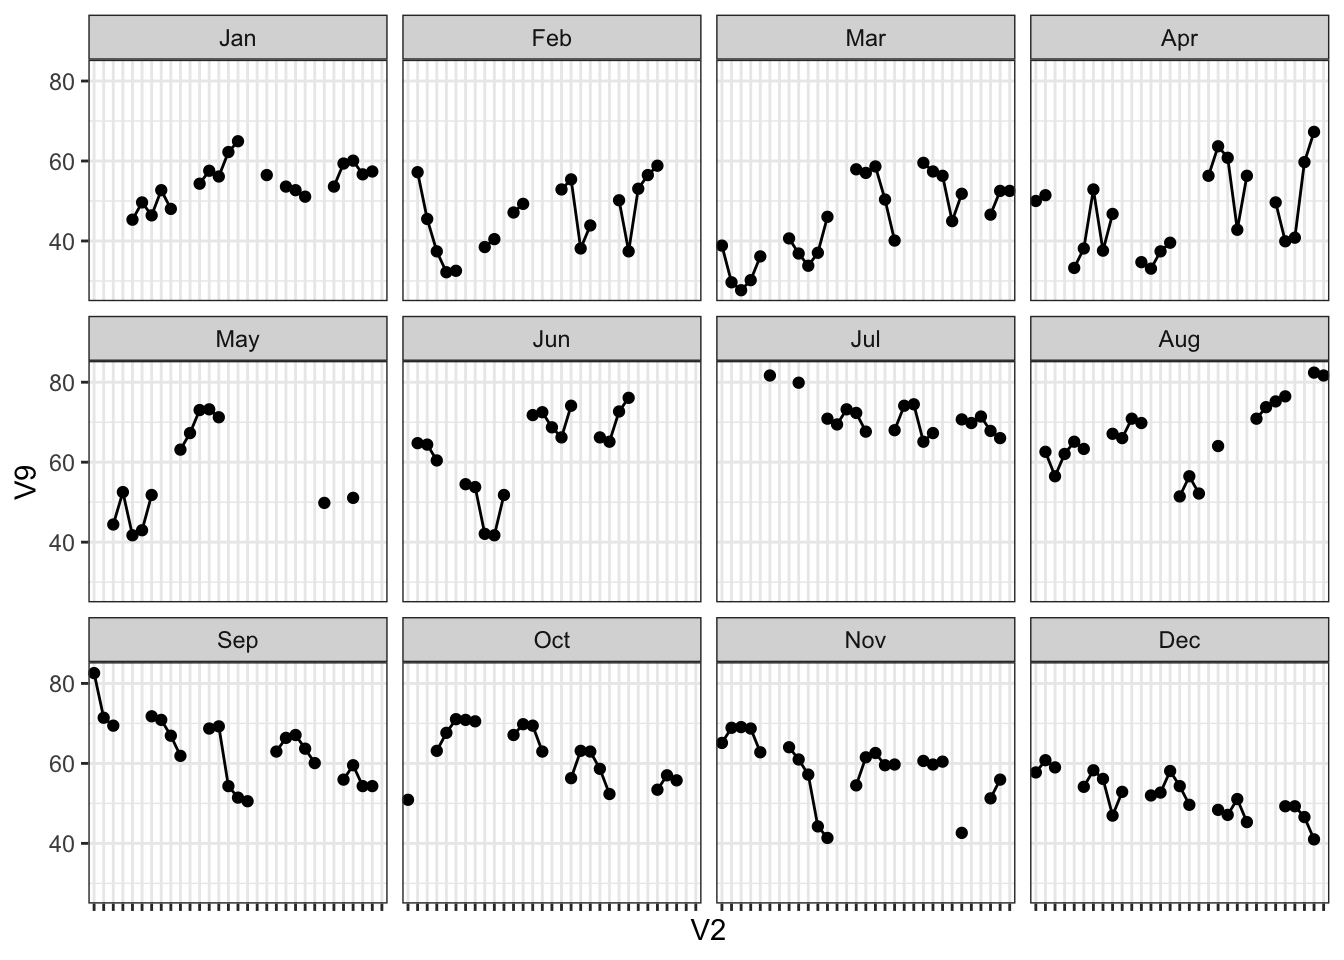
\includegraphics{_main_files/figure-latex/unnamed-chunk-169-1.pdf}

Adding multiple trendlines is easy using the \texttt{group\ =} aesthetic within \texttt{geom\_line()}; here I will plot \texttt{V7} and \texttt{V11} together - humidity and pressure gradient measured at LAX, respectively:

\begin{Shaded}
\begin{Highlighting}[]
\NormalTok{df\_2 }\OtherTok{\textless{}{-}}\NormalTok{ df }\SpecialCharTok{\%\textgreater{}\%} \FunctionTok{select}\NormalTok{(V1, V2, V7, V11) }\SpecialCharTok{\%\textgreater{}\%}
  \FunctionTok{pivot\_longer}\NormalTok{(}\FunctionTok{c}\NormalTok{(V7, V11), }
               \AttributeTok{names\_to =} \StringTok{\textquotesingle{}Measurement\textquotesingle{}}\NormalTok{, }
               \AttributeTok{values\_to =} \StringTok{\textquotesingle{}Values\textquotesingle{}}\NormalTok{)}

\FunctionTok{ggplot}\NormalTok{(df\_2, }\FunctionTok{aes}\NormalTok{(}\AttributeTok{x =}\NormalTok{ V2, }\AttributeTok{y =}\NormalTok{ Values)) }\SpecialCharTok{+}
  \FunctionTok{geom\_point}\NormalTok{() }\SpecialCharTok{+} 
  \FunctionTok{geom\_line}\NormalTok{(}\FunctionTok{aes}\NormalTok{(}\AttributeTok{group =}\NormalTok{ Measurement,}
                \AttributeTok{color =}\NormalTok{ Measurement)) }\SpecialCharTok{+}
  \FunctionTok{facet\_wrap}\NormalTok{(}\SpecialCharTok{\textasciitilde{}}\NormalTok{ V1) }\SpecialCharTok{+} \FunctionTok{theme\_bw}\NormalTok{() }\SpecialCharTok{+} 
  \FunctionTok{theme}\NormalTok{(}\AttributeTok{legend.position =} \StringTok{\textquotesingle{}bottom\textquotesingle{}}\NormalTok{,}
        \AttributeTok{axis.text.x =} \FunctionTok{element\_blank}\NormalTok{())}
\end{Highlighting}
\end{Shaded}

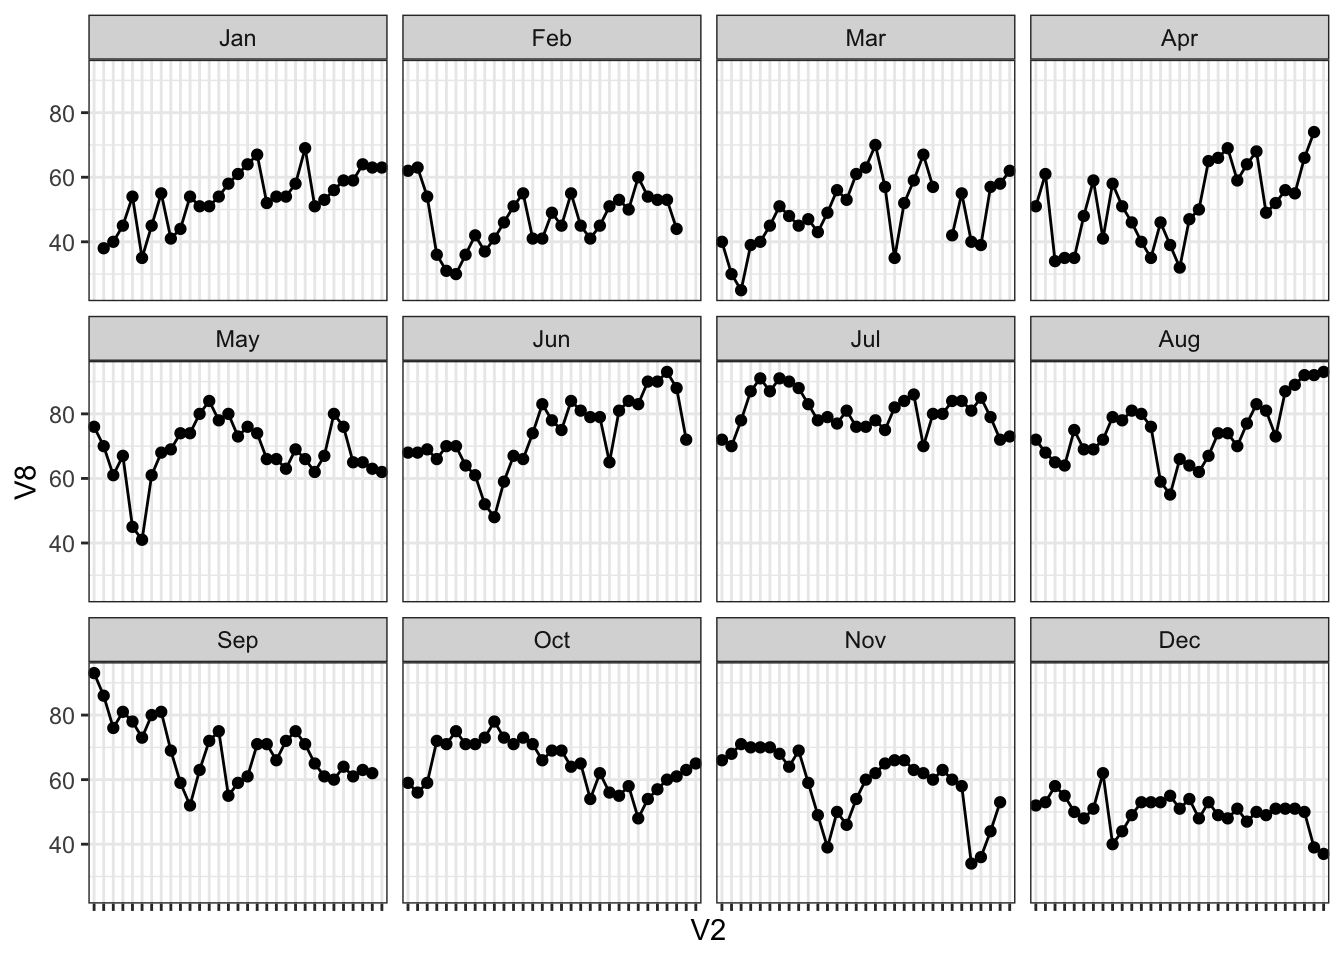
\includegraphics{_main_files/figure-latex/unnamed-chunk-170-1.pdf}

Working with grouped data such as this means an ANOVA tells us whether there is a significant variation across the group means relative to the within-group means:

\begin{Shaded}
\begin{Highlighting}[]
\NormalTok{aov\_mod }\OtherTok{\textless{}{-}} \FunctionTok{aov}\NormalTok{(V8 }\SpecialCharTok{\textasciitilde{}}\NormalTok{ V1, }\AttributeTok{data =}\NormalTok{ df)}
\FunctionTok{summary}\NormalTok{(aov\_mod)}
\end{Highlighting}
\end{Shaded}

\begin{verbatim}
##              Df Sum Sq Mean Sq F value Pr(>F)    
## V1           11  43504    3955   45.67 <2e-16 ***
## Residuals   352  30483      87                   
## ---
## Signif. codes:  
## 0 '***' 0.001 '**' 0.01 '*' 0.05 '.' 0.1 ' ' 1
## 2 observations deleted due to missingness
\end{verbatim}

A nice way to visualize an ANOVA result is by using grouped boxplots; here I am adding the Kruskal-Wallis ANOVA result from \texttt{ggpubr()}:

\begin{Shaded}
\begin{Highlighting}[]
\FunctionTok{ggplot}\NormalTok{(df, }\FunctionTok{aes}\NormalTok{(}\AttributeTok{x =}\NormalTok{ V1, }\AttributeTok{y =}\NormalTok{ V8)) }\SpecialCharTok{+}
  \FunctionTok{geom\_boxplot}\NormalTok{(}\FunctionTok{aes}\NormalTok{(}\AttributeTok{fill =}\NormalTok{ V1), }\AttributeTok{alpha =}\NormalTok{ .}\DecValTok{6}\NormalTok{) }\SpecialCharTok{+}
  \FunctionTok{theme\_bw}\NormalTok{() }\SpecialCharTok{+} \FunctionTok{xlab}\NormalTok{(}\StringTok{\textquotesingle{}\textquotesingle{}}\NormalTok{) }\SpecialCharTok{+}
  \FunctionTok{theme}\NormalTok{(}\AttributeTok{legend.position =} \StringTok{\textquotesingle{}none\textquotesingle{}}\NormalTok{) }\SpecialCharTok{+}
  \FunctionTok{stat\_compare\_means}\NormalTok{(}\AttributeTok{method =} \StringTok{\textquotesingle{}kruskal\textquotesingle{}}\NormalTok{)}
\end{Highlighting}
\end{Shaded}

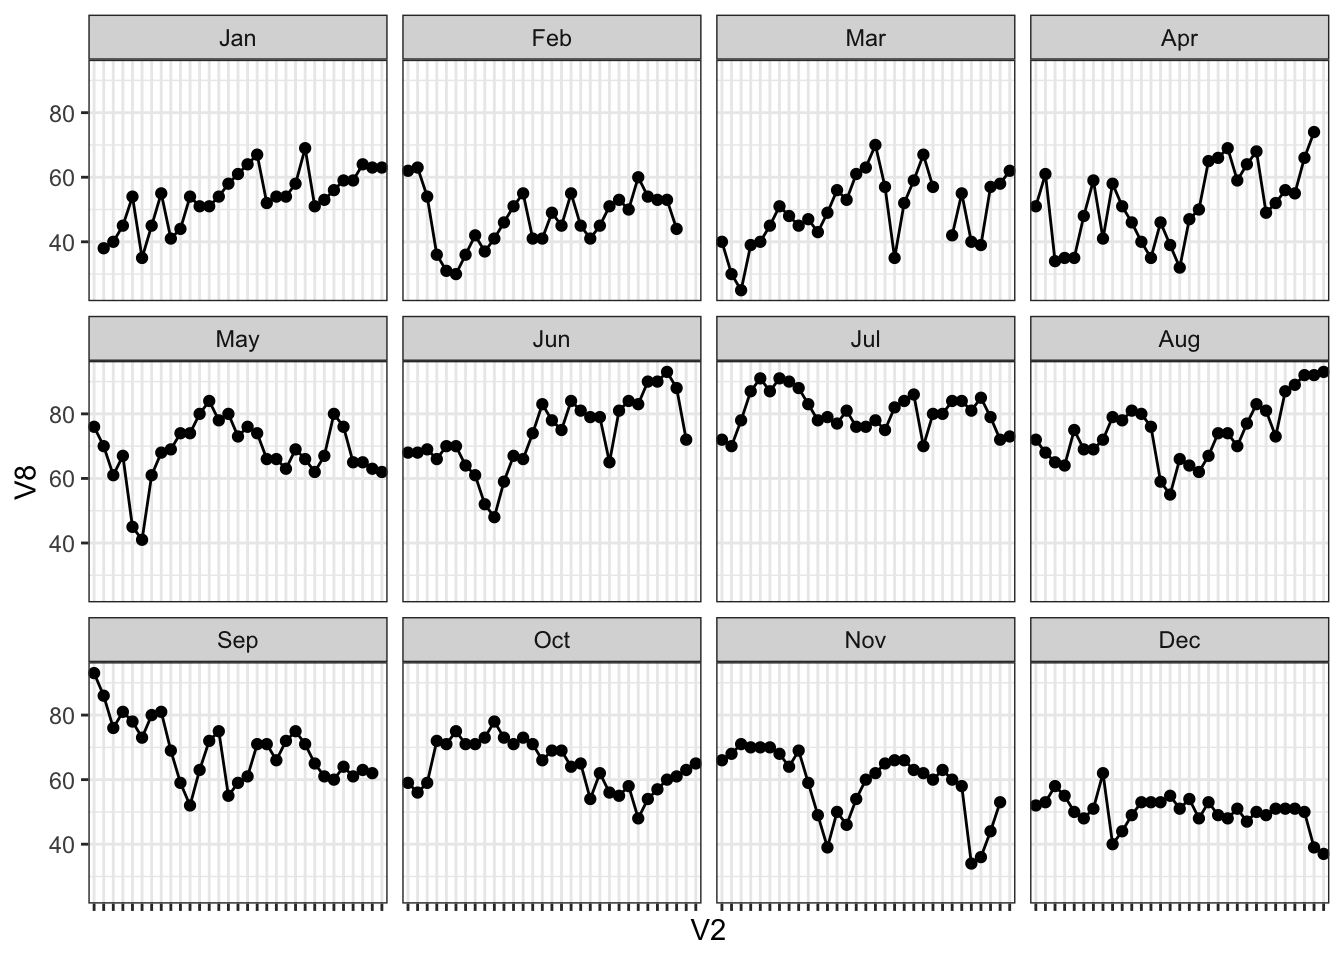
\includegraphics{_main_files/figure-latex/unnamed-chunk-172-1.pdf}

Instead of an ANOVA, I can also run pairwise Wilcoxon tests against a reference group. Here I will make January the reference group:

\begin{Shaded}
\begin{Highlighting}[]
\FunctionTok{ggplot}\NormalTok{(df, }\FunctionTok{aes}\NormalTok{(}\AttributeTok{x =}\NormalTok{ V1, }\AttributeTok{y =}\NormalTok{ V8)) }\SpecialCharTok{+}
  \FunctionTok{geom\_boxplot}\NormalTok{(}\FunctionTok{aes}\NormalTok{(}\AttributeTok{fill =}\NormalTok{ V1), }\AttributeTok{alpha =}\NormalTok{ .}\DecValTok{6}\NormalTok{) }\SpecialCharTok{+}
  \FunctionTok{theme\_bw}\NormalTok{() }\SpecialCharTok{+} \FunctionTok{xlab}\NormalTok{(}\StringTok{\textquotesingle{}\textquotesingle{}}\NormalTok{) }\SpecialCharTok{+}
  \FunctionTok{theme}\NormalTok{(}\AttributeTok{legend.position =} \StringTok{\textquotesingle{}none\textquotesingle{}}\NormalTok{) }\SpecialCharTok{+}
  \FunctionTok{stat\_compare\_means}\NormalTok{(}\AttributeTok{method =} \StringTok{\textquotesingle{}wilcox\textquotesingle{}}\NormalTok{,}
                     \AttributeTok{ref.group =} \StringTok{\textquotesingle{}Jan\textquotesingle{}}\NormalTok{,}
                     \AttributeTok{label =} \StringTok{\textquotesingle{}p.signif\textquotesingle{}}\NormalTok{)}
\end{Highlighting}
\end{Shaded}

\begin{verbatim}
## Warning: The dot-dot notation (`..p.signif..`) was deprecated in
## ggplot2 3.4.0.
## i Please use `after_stat(p.signif)` instead.
\end{verbatim}

\begin{verbatim}
## Warning: Removed 2 rows containing non-finite values
## (`stat_boxplot()`).
\end{verbatim}

\begin{verbatim}
## Warning: Removed 2 rows containing non-finite values
## (`stat_compare_means()`).
\end{verbatim}

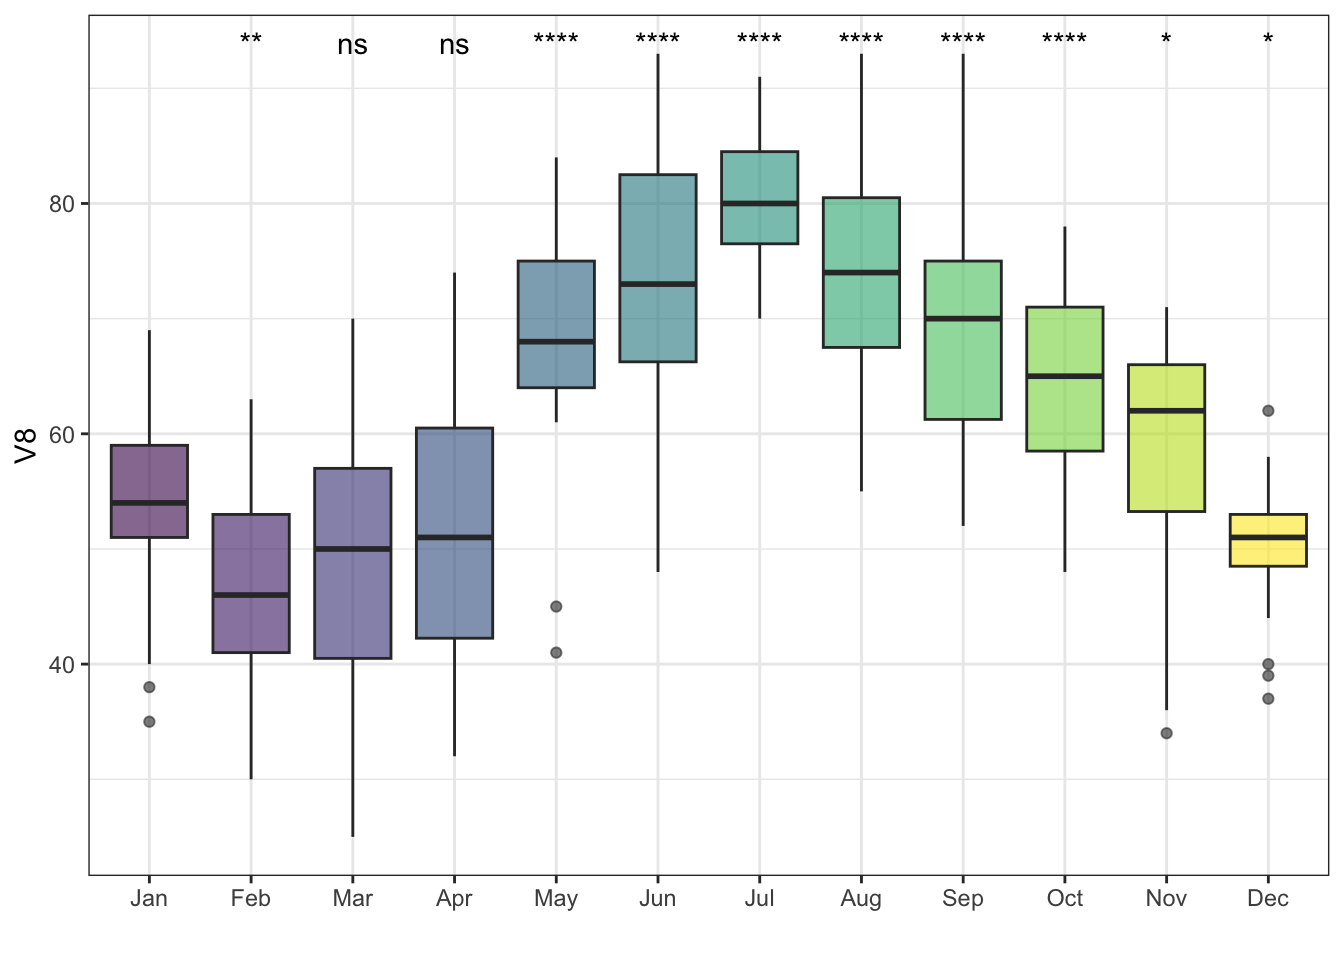
\includegraphics{_main_files/figure-latex/unnamed-chunk-173-1.pdf}

If we want to calculate values based on groups, \texttt{dplyr}'s \texttt{group\_by()} is useful, as seen in Chapter 1:

\begin{Shaded}
\begin{Highlighting}[]
\NormalTok{df }\SpecialCharTok{\%\textgreater{}\%} \FunctionTok{group\_by}\NormalTok{(V1) }\SpecialCharTok{\%\textgreater{}\%}
  \FunctionTok{summarise}\NormalTok{(}\FunctionTok{across}\NormalTok{(V4}\SpecialCharTok{:}\NormalTok{V13, }\SpecialCharTok{\textasciitilde{}} \FunctionTok{mean}\NormalTok{(.x, }\AttributeTok{na.rm =} \ConstantTok{TRUE}\NormalTok{), }
                   \AttributeTok{.names =} \StringTok{\textquotesingle{}mean\_\{col\}\textquotesingle{}}\NormalTok{))}
\end{Highlighting}
\end{Shaded}

\begin{verbatim}
## # A tibble: 12 x 11
##    V1    mean_V4 mean_V5 mean_V6 mean_V7 mean_V8 mean_V9
##    <ord>   <dbl>   <dbl>   <dbl>   <dbl>   <dbl>   <dbl>
##  1 Jan      5.45   5745.    4.23    37.4    53.7    54.6
##  2 Feb      7.14   5659.    5.69    56.9    47.0    45.9
##  3 Mar      8.84   5656.    5.03    49.8    49.5    45.3
##  4 Apr     10      5637.    5.97    58.2    51.7    47.2
##  5 May     15.8    5753.    5.48    70.9    68.4    56.9
##  6 Jun     17.1    5792     5.2     63.3    73.6    62.8
##  7 Jul     20.2    5862.    5.29    72.8    80.5    71.2
##  8 Aug     17.5    5830.    5.23    67.6    74.4    66.7
##  9 Sep     12.4    5797.    5.77    73.6    69.2    63.5
## 10 Oct     12.6    5796.    4.90    62.7    64.5    62.4
## 11 Nov      7.67   5790.    3.3     50.1    58.8    58.6
## 12 Dec      4.06   5725     2.42    36.1    50.2    51.9
## # ... with 4 more variables: mean_V10 <dbl>, mean_V11 <dbl>,
## #   mean_V12 <dbl>, mean_V13 <dbl>
\end{verbatim}

\begin{Shaded}
\begin{Highlighting}[]
\NormalTok{df }\SpecialCharTok{\%\textgreater{}\%} \FunctionTok{group\_by}\NormalTok{(V1, V3) }\SpecialCharTok{\%\textgreater{}\%}
  \FunctionTok{summarise}\NormalTok{(}\AttributeTok{mean\_hum\_LAX =} \FunctionTok{mean}\NormalTok{(V7, }\AttributeTok{na.rm=}\NormalTok{T))}
\end{Highlighting}
\end{Shaded}

\begin{verbatim}
## `summarise()` has grouped output by 'V1'. You can override
## using the `.groups` argument.
\end{verbatim}

\begin{verbatim}
## # A tibble: 84 x 3
## # Groups:   V1 [12]
##    V1    V3        mean_hum_LAX
##    <ord> <fct>            <dbl>
##  1 Jan   Monday            56  
##  2 Jan   Tuesday           35  
##  3 Jan   Wednesday         19  
##  4 Jan   Thursday          21.8
##  5 Jan   Friday            44.8
##  6 Jan   Saturday          41.6
##  7 Jan   Sunday            46.8
##  8 Feb   Monday            58.2
##  9 Feb   Tuesday           69.2
## 10 Feb   Wednesday         63.2
## # ... with 74 more rows
\end{verbatim}

\hypertarget{visualization-of-clusters}{%
\section{Visualization of clusters}\label{visualization-of-clusters}}

Clustering and dimensionality reduction tasks can give us a visual look at groupings in the data. The concept of unsupervised clustering and dimensionality reduction techniques will be covered in one of the future chapters, but this is a high-level glance that will be useful in quickly identifying clusters:

\begin{Shaded}
\begin{Highlighting}[]
\FunctionTok{data}\NormalTok{(}\StringTok{"iris"}\NormalTok{)}
\NormalTok{df }\OtherTok{\textless{}{-}} \FunctionTok{as\_tibble}\NormalTok{(iris)}
\end{Highlighting}
\end{Shaded}

For PCA, I will use the useful \texttt{factoextra} package for visualization. The first step is to make sure that the input for PCA is numeric; this means that, for example, in the \texttt{iris} dataset, I need to exclude the column containing the target labels. Additionally, I am declaring the target label column as a factor, since I want to label the data points with these labels in the PCA plot.

The \texttt{fviz\_pca\_ind()} function draws the PCA plot:

\begin{Shaded}
\begin{Highlighting}[]
\FunctionTok{library}\NormalTok{(factoextra)}

\NormalTok{pc\_res }\OtherTok{\textless{}{-}} \FunctionTok{prcomp}\NormalTok{(}
\NormalTok{  df }\SpecialCharTok{\%\textgreater{}\%} \FunctionTok{select}\NormalTok{(}\SpecialCharTok{{-}}\NormalTok{Species), }\AttributeTok{scale =} \ConstantTok{TRUE}
\NormalTok{)}

\NormalTok{groups }\OtherTok{\textless{}{-}} \FunctionTok{factor}\NormalTok{(df}\SpecialCharTok{$}\NormalTok{Species)}

\FunctionTok{fviz\_pca\_ind}\NormalTok{(pc\_res, }\AttributeTok{col.ind =}\NormalTok{ groups, }
             \AttributeTok{addEllipses =} \ConstantTok{TRUE}\NormalTok{, }
             \AttributeTok{legend.title =} \StringTok{\textquotesingle{}Species\textquotesingle{}}\NormalTok{)}
\end{Highlighting}
\end{Shaded}

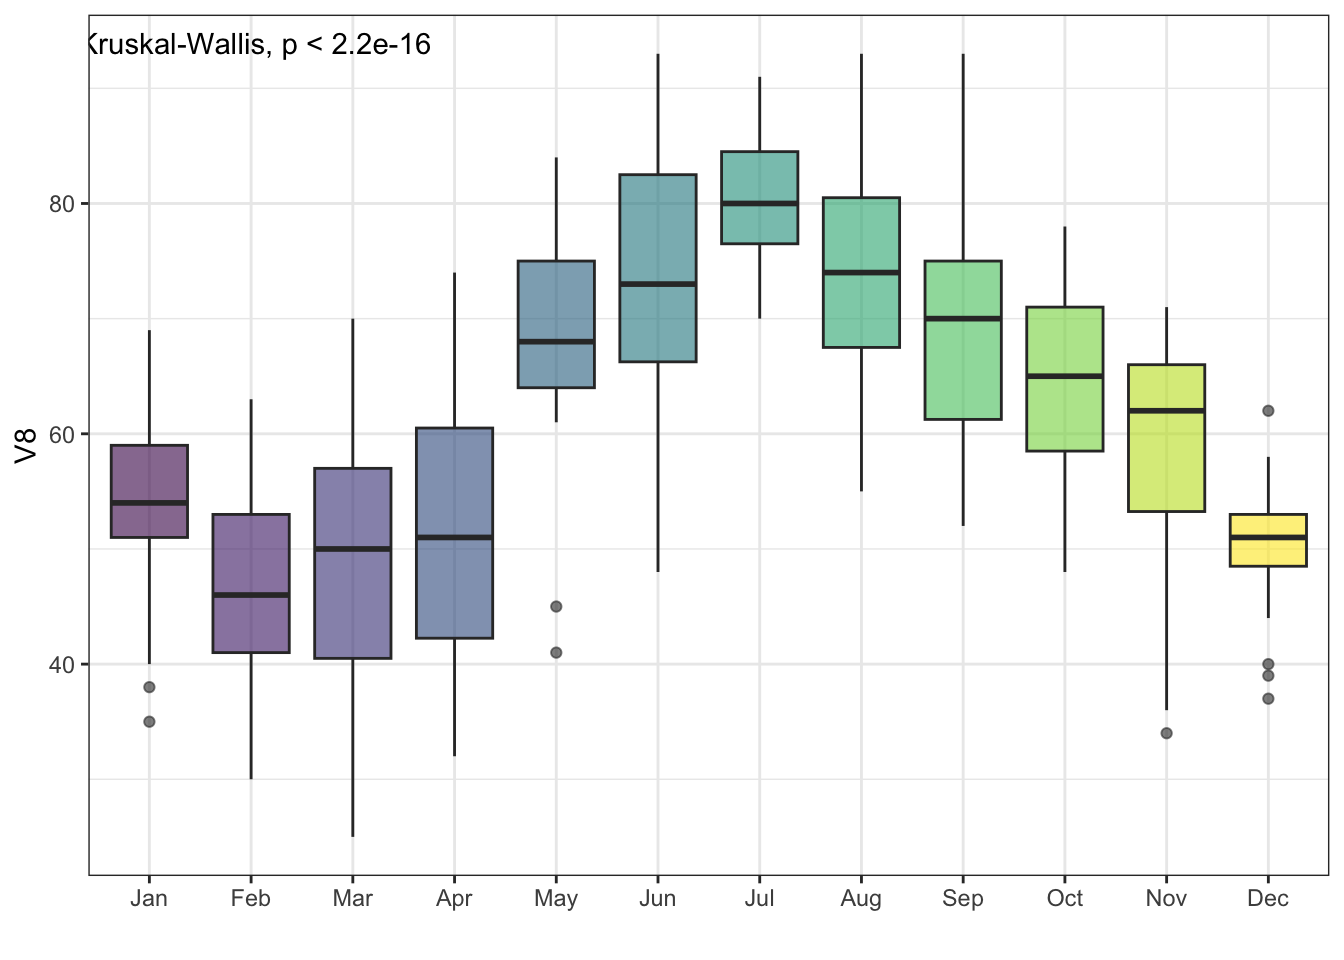
\includegraphics{_main_files/figure-latex/unnamed-chunk-177-1.pdf}

Since this is a tiny and simple dataset frequently used in these types of tutorials, it's no surprise that we get nice ellipses in the data. The data points separate well across the first PC (the x-axis).

The \texttt{fviz\_contrib()} plot shows the contribution of each variable. The horizontal red line here shows the expected level of contribution if the contributions were uniform. The \texttt{axes\ =\ 1} argument states that I want to check for the contribution in the first PC only.

\begin{Shaded}
\begin{Highlighting}[]
\FunctionTok{fviz\_contrib}\NormalTok{(pc\_res, }\AttributeTok{axes =} \DecValTok{1}\NormalTok{, }\AttributeTok{choice =} \StringTok{\textquotesingle{}var\textquotesingle{}}\NormalTok{)}
\end{Highlighting}
\end{Shaded}

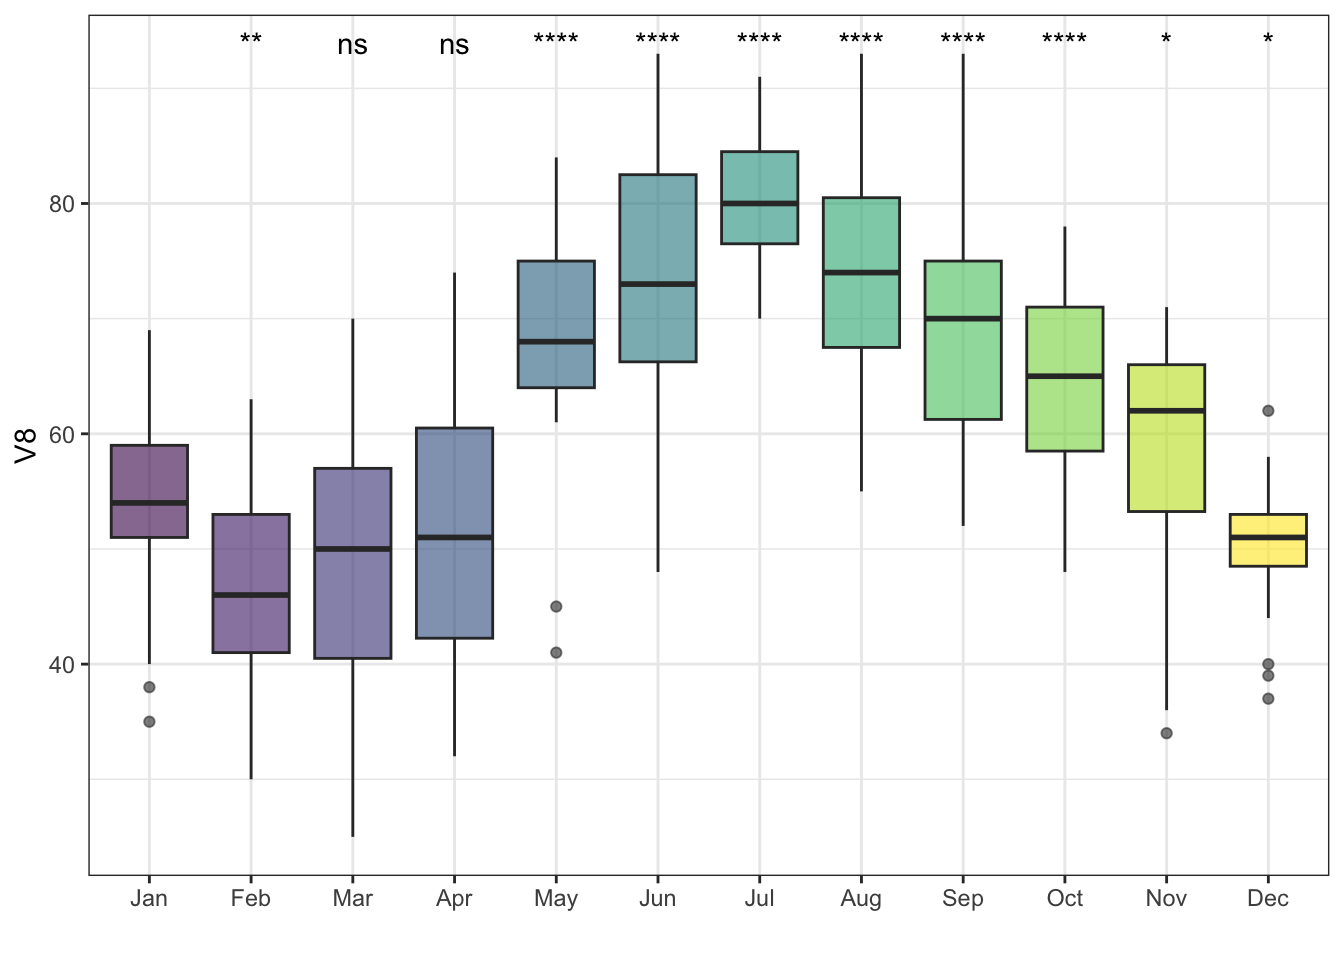
\includegraphics{_main_files/figure-latex/unnamed-chunk-178-1.pdf}

Screeplot shows the level of covariance explained by each PC:

\begin{Shaded}
\begin{Highlighting}[]
\FunctionTok{fviz\_screeplot}\NormalTok{(pc\_res)}
\end{Highlighting}
\end{Shaded}

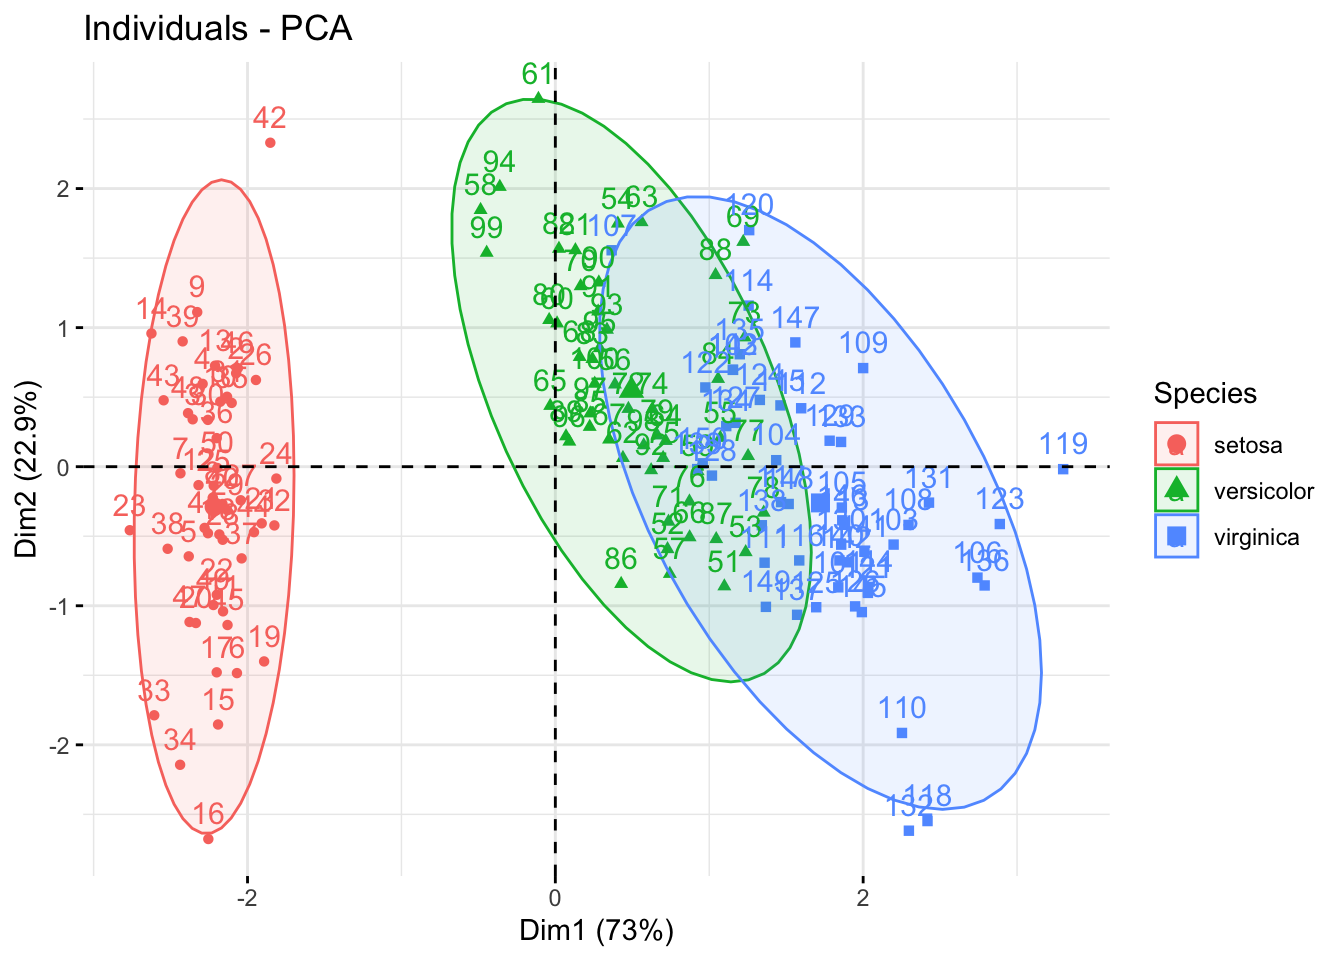
\includegraphics{_main_files/figure-latex/unnamed-chunk-179-1.pdf}

Alternatively, dendrograms are a commonly used tools to visualize hierarchical clustering in the data. Again, the concept behind the clustering method will be explained in greater detail in future chapters, but essentially we need to generate a distance matrix (using some sort of a distance metric, in this case Euclidean distance) and then calculate linkage between each instance. The \texttt{dist()} and \texttt{hclust()} from base R handles this nicely:

\begin{Shaded}
\begin{Highlighting}[]
\FunctionTok{data}\NormalTok{(mtcars)}

\NormalTok{dm }\OtherTok{\textless{}{-}} \FunctionTok{dist}\NormalTok{(mtcars, }\AttributeTok{method =} \StringTok{\textquotesingle{}euclidean\textquotesingle{}}\NormalTok{)}
\NormalTok{hc }\OtherTok{\textless{}{-}} \FunctionTok{hclust}\NormalTok{(dm, }\AttributeTok{method =} \StringTok{\textquotesingle{}complete\textquotesingle{}}\NormalTok{)}
\end{Highlighting}
\end{Shaded}

The \texttt{dendextend} package can accept the output from \texttt{hclust} to make customizable dendrograms:

\begin{Shaded}
\begin{Highlighting}[]
\FunctionTok{library}\NormalTok{(dendextend)}
\NormalTok{den }\OtherTok{\textless{}{-}} \FunctionTok{as.dendrogram}\NormalTok{(hc)}

\NormalTok{den }\SpecialCharTok{\%\textgreater{}\%} \FunctionTok{plot}\NormalTok{()}
\end{Highlighting}
\end{Shaded}

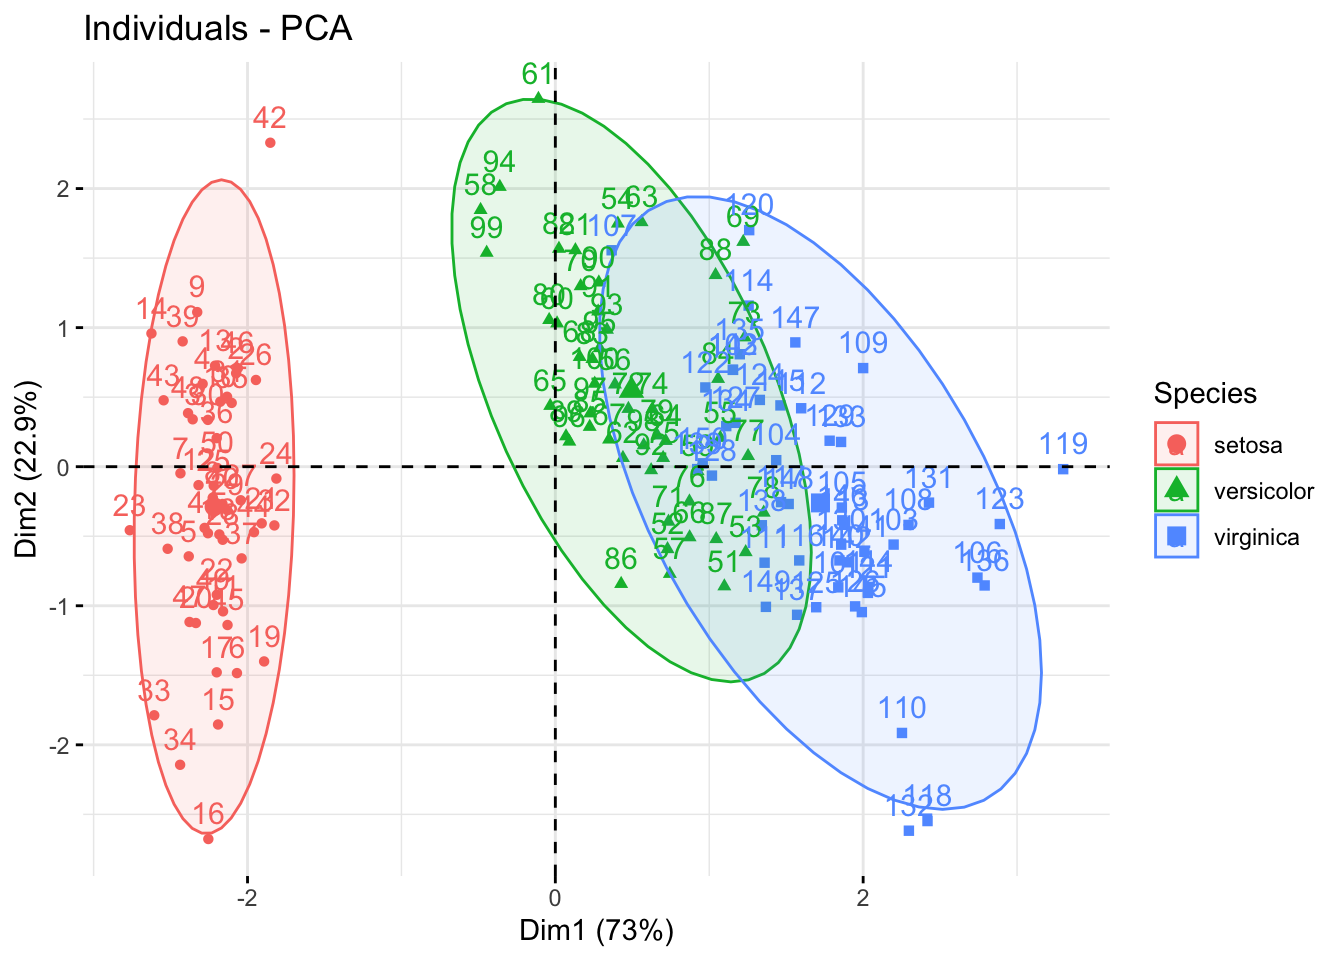
\includegraphics{_main_files/figure-latex/unnamed-chunk-181-1.pdf}

When we know the number of clusters present, we can color them differently with \texttt{color\_branches()}. For an alternative look at dendrograms, we can circlize them using \texttt{circlize\_dendrogram()}:

\begin{Shaded}
\begin{Highlighting}[]
\NormalTok{den }\SpecialCharTok{\%\textgreater{}\%} \FunctionTok{color\_branches}\NormalTok{(}\AttributeTok{k =} \DecValTok{4}\NormalTok{) }\SpecialCharTok{\%\textgreater{}\%}
  \FunctionTok{circlize\_dendrogram}\NormalTok{()}
\end{Highlighting}
\end{Shaded}

\begin{verbatim}
## Loading required namespace: circlize
\end{verbatim}

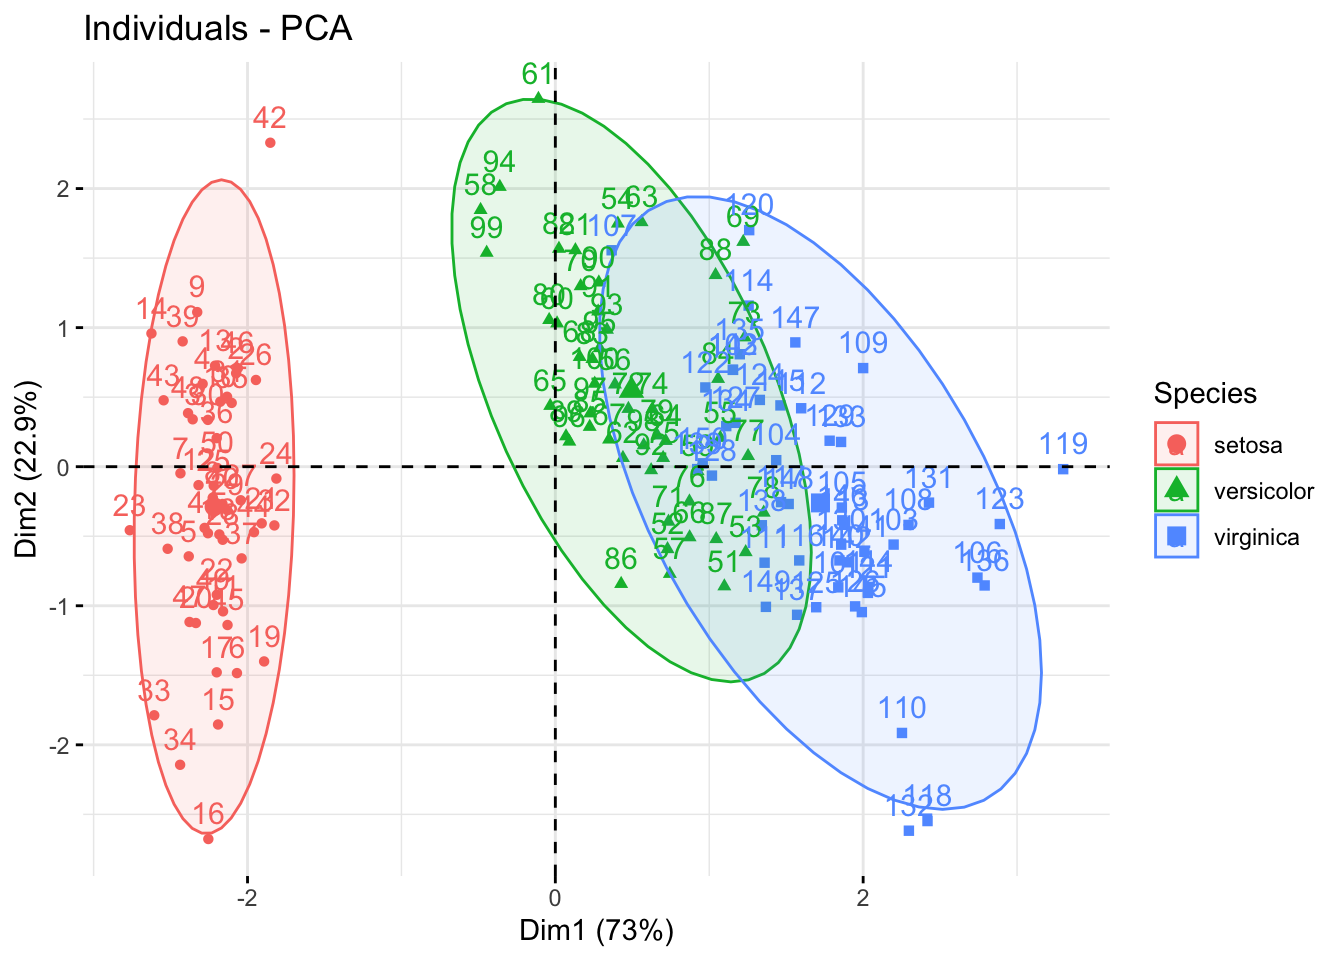
\includegraphics{_main_files/figure-latex/unnamed-chunk-182-1.pdf}

The \texttt{cutree()} function accepts the \texttt{hclust()} output and assigns a cluster label, depending on the number of clusters defined:

\begin{Shaded}
\begin{Highlighting}[]
\FunctionTok{cutree}\NormalTok{(hc, }\AttributeTok{k =} \DecValTok{4}\NormalTok{) }\SpecialCharTok{\%\textgreater{}\%} \FunctionTok{head}\NormalTok{()}
\end{Highlighting}
\end{Shaded}

\begin{verbatim}
##         Mazda RX4     Mazda RX4 Wag        Datsun 710 
##                 1                 1                 1 
##    Hornet 4 Drive Hornet Sportabout           Valiant 
##                 2                 3                 2
\end{verbatim}

Finally, identifying the optimal number of clusters in the data can mainly be done using the silhouette method or the elbow (also called the wss) method:

\begin{Shaded}
\begin{Highlighting}[]
\FunctionTok{fviz\_nbclust}\NormalTok{(mtcars, }\AttributeTok{FUNcluster =}\NormalTok{ hcut,}
             \AttributeTok{method =} \StringTok{\textquotesingle{}silhouette\textquotesingle{}}\NormalTok{,}
             \AttributeTok{diss =}\NormalTok{ dm)}
\end{Highlighting}
\end{Shaded}

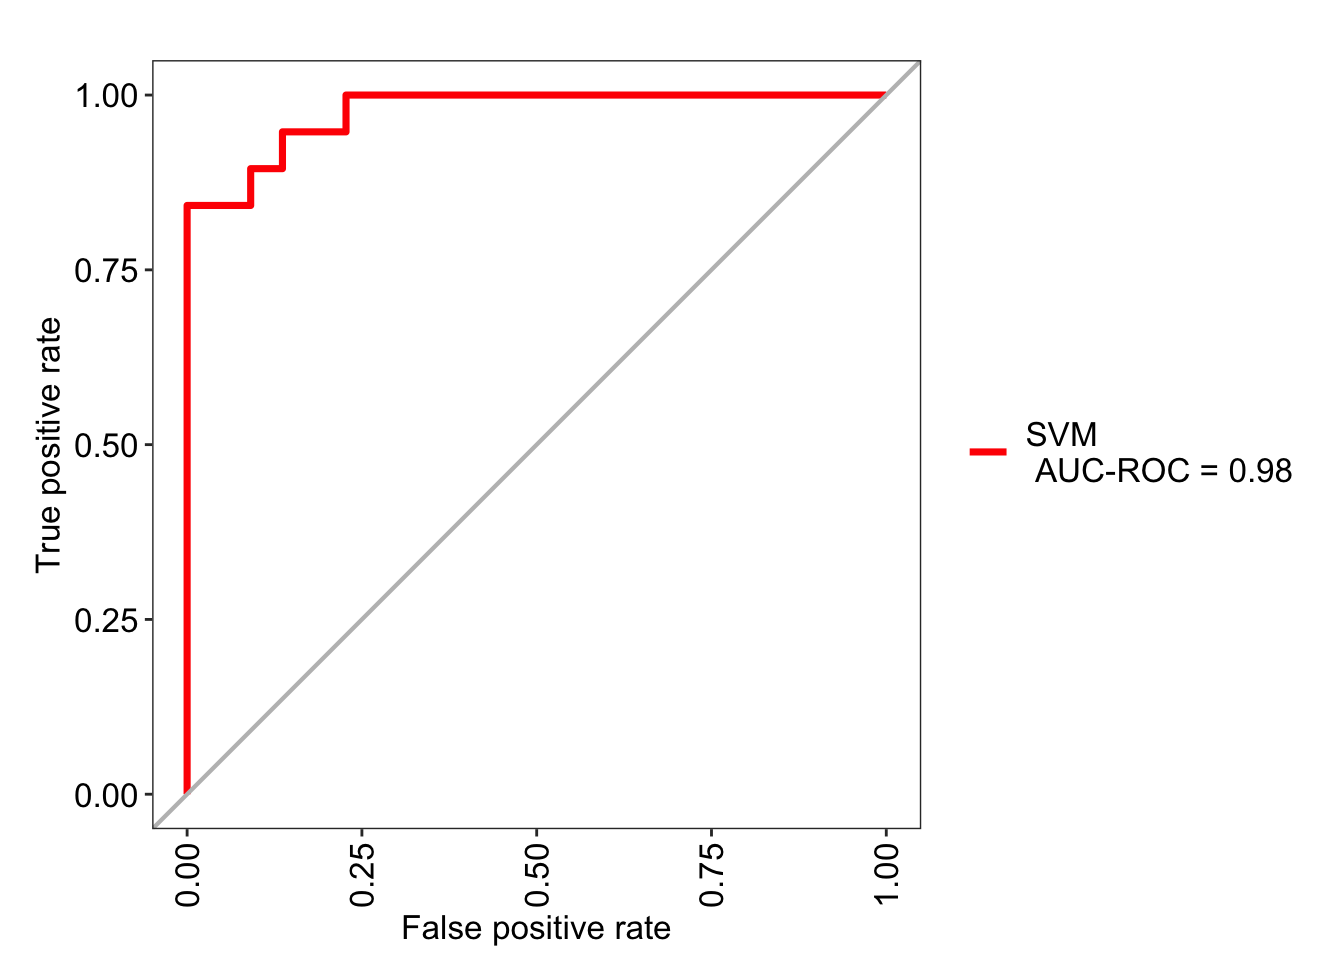
\includegraphics{_main_files/figure-latex/unnamed-chunk-184-1.pdf}

\begin{Shaded}
\begin{Highlighting}[]
\FunctionTok{fviz\_nbclust}\NormalTok{(mtcars, }\AttributeTok{FUNcluster =}\NormalTok{ hcut,}
             \AttributeTok{method =} \StringTok{\textquotesingle{}wss\textquotesingle{}}\NormalTok{,}
             \AttributeTok{diss =}\NormalTok{ dm)}
\end{Highlighting}
\end{Shaded}

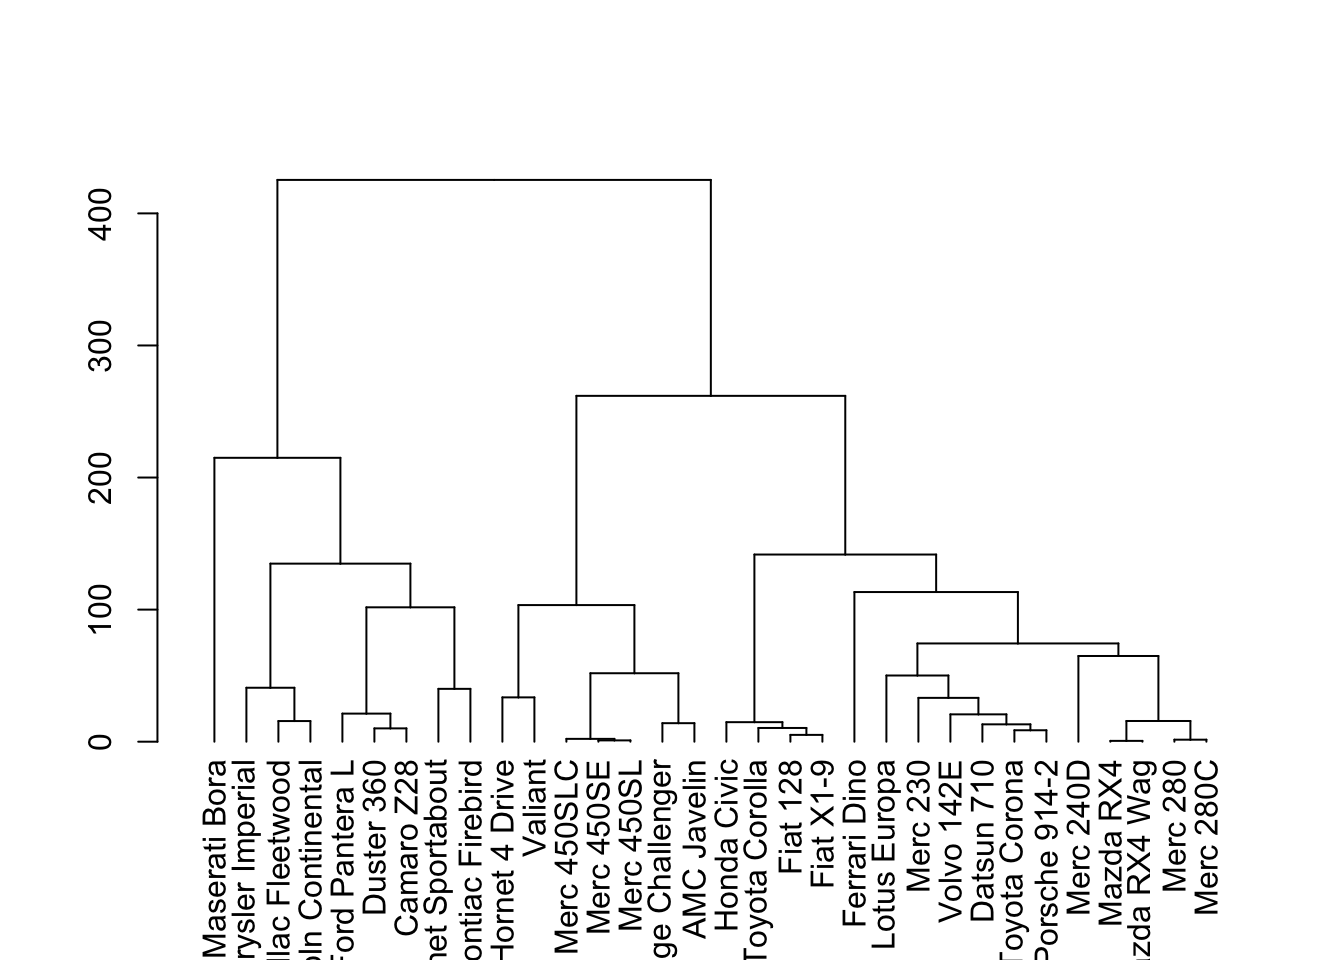
\includegraphics{_main_files/figure-latex/unnamed-chunk-185-1.pdf}

\hypertarget{everyday-ml-classification}{%
\chapter{Everyday ML: Classification}\label{everyday-ml-classification}}

In the preceeding chapters, I reviewed the fundamentals of wrangling data as well as running some exploratory data analysis to get a feel for the data at hand. In data science projects, it is often typical to frame problems in context of a model - how does a variable \emph{y} behave according to some other variable \emph{x}? For example, how does the pricing of a residential property behave according to the square footage? Is the relationship linear? Are there confounding variables that affect this relationship we have not accounted for?

In the simplest sense, fitting a linear model using ordinary least squares using \texttt{lm()} in R provide us with two parameters: the coefficient and the intercept. We can use these parameters to predict the housing price of a property based on the input \emph{feature} - or \emph{features} most likely - of that particular instance. This is the fundamental concept at the core of supervised learning. This example is a type of a \emph{regression} as the target variable (i.e., the housing price) is a continuous variable. However, if the variable we were trying to predict is categorical (e.g., bins based on the bracket of housing price) the task would be \emph{classification}.

The digression into concepts in ML and the details into each algorithm is beyond the scope of this book, but more details around specific topics are available on my \href{https://brianjmpark.github.io/}{blog} as well as documentation for popular ML packages such as Python's \href{https://scikit-learn.org/stable/}{Scikit-Learn}.

In R, the workhorse of supervised learning models, whether it's classification or regression, is the \texttt{caret} package.

\begin{Shaded}
\begin{Highlighting}[]
\FunctionTok{library}\NormalTok{(tidyverse)}
\FunctionTok{library}\NormalTok{(caret)}
\end{Highlighting}
\end{Shaded}

\begin{verbatim}
## Loading required package: lattice
\end{verbatim}

\begin{verbatim}
## 
## Attaching package: 'caret'
\end{verbatim}

\begin{verbatim}
## The following object is masked from 'package:purrr':
## 
##     lift
\end{verbatim}

\hypertarget{model-training-and-predictions}{%
\section{Model training and predictions}\label{model-training-and-predictions}}

For the first exercise I will use a dataset from Kaggle \href{https://www.kaggle.com/datasets/kkhandekar/all-datasets-for-practicing-ml}{here} which I also uploaded onto my GitHub for reference:

\begin{Shaded}
\begin{Highlighting}[]
\NormalTok{url }\OtherTok{\textless{}{-}} \StringTok{\textquotesingle{}https://raw.githubusercontent.com/snowoflondon/everyday{-}r/main/datasets/Class\_Winequality.csv\textquotesingle{}}
\NormalTok{df }\OtherTok{\textless{}{-}} \FunctionTok{read\_delim}\NormalTok{(url, }\AttributeTok{delim =} \StringTok{\textquotesingle{};\textquotesingle{}}\NormalTok{)}
\end{Highlighting}
\end{Shaded}

\begin{verbatim}
## 
## -- Column specification -------------------------------------
## cols(
##   `fixed acidity` = col_double(),
##   `volatile acidity` = col_double(),
##   `citric acid` = col_double(),
##   `residual sugar` = col_double(),
##   chlorides = col_double(),
##   `free sulfur dioxide` = col_double(),
##   `total sulfur dioxide` = col_double(),
##   density = col_double(),
##   pH = col_double(),
##   sulphates = col_double(),
##   alcohol = col_double(),
##   quality = col_double()
## )
\end{verbatim}

\begin{Shaded}
\begin{Highlighting}[]
\FunctionTok{head}\NormalTok{(df)}
\end{Highlighting}
\end{Shaded}

\begin{verbatim}
## # A tibble: 6 x 12
##   fixed aci~1 volat~2 citri~3 resid~4 chlor~5 free ~6 total~7
##         <dbl>   <dbl>   <dbl>   <dbl>   <dbl>   <dbl>   <dbl>
## 1         7      0.27    0.36    20.7   0.045      45     170
## 2         6.3    0.3     0.34     1.6   0.049      14     132
## 3         8.1    0.28    0.4      6.9   0.05       30      97
## 4         7.2    0.23    0.32     8.5   0.058      47     186
## 5         7.2    0.23    0.32     8.5   0.058      47     186
## 6         8.1    0.28    0.4      6.9   0.05       30      97
## # ... with 5 more variables: density <dbl>, pH <dbl>,
## #   sulphates <dbl>, alcohol <dbl>, quality <dbl>, and
## #   abbreviated variable names 1: `fixed acidity`,
## #   2: `volatile acidity`, 3: `citric acid`,
## #   4: `residual sugar`, 5: chlorides,
## #   6: `free sulfur dioxide`, 7: `total sulfur dioxide`
\end{verbatim}

This dataset has 11 features and a target label column called \texttt{quality}. Firstly, I convert the \texttt{quality} column into factors to reiterate the fact that we are working with a categorical column with defined levels.

\begin{Shaded}
\begin{Highlighting}[]
\NormalTok{df }\OtherTok{\textless{}{-}}\NormalTok{ df }\SpecialCharTok{\%\textgreater{}\%} \FunctionTok{mutate}\NormalTok{(}\AttributeTok{quality =} \FunctionTok{factor}\NormalTok{(quality)) }\SpecialCharTok{\%\textgreater{}\%} \FunctionTok{relocate}\NormalTok{(quality)}
\end{Highlighting}
\end{Shaded}

A glimpse into the 11 features shows us that the values are heterogenous in scale:

\begin{Shaded}
\begin{Highlighting}[]
\FunctionTok{summary}\NormalTok{(df }\SpecialCharTok{\%\textgreater{}\%} \FunctionTok{select}\NormalTok{(}\SpecialCharTok{{-}}\NormalTok{quality))}
\end{Highlighting}
\end{Shaded}

\begin{verbatim}
##  fixed acidity    volatile acidity  citric acid    
##  Min.   : 3.800   Min.   :0.0800   Min.   :0.0000  
##  1st Qu.: 6.300   1st Qu.:0.2100   1st Qu.:0.2700  
##  Median : 6.800   Median :0.2600   Median :0.3200  
##  Mean   : 6.855   Mean   :0.2782   Mean   :0.3342  
##  3rd Qu.: 7.300   3rd Qu.:0.3200   3rd Qu.:0.3900  
##  Max.   :14.200   Max.   :1.1000   Max.   :1.6600  
##  residual sugar     chlorides       free sulfur dioxide
##  Min.   : 0.600   Min.   :0.00900   Min.   :  2.00     
##  1st Qu.: 1.700   1st Qu.:0.03600   1st Qu.: 23.00     
##  Median : 5.200   Median :0.04300   Median : 34.00     
##  Mean   : 6.391   Mean   :0.04577   Mean   : 35.31     
##  3rd Qu.: 9.900   3rd Qu.:0.05000   3rd Qu.: 46.00     
##  Max.   :65.800   Max.   :0.34600   Max.   :289.00     
##  total sulfur dioxide    density             pH       
##  Min.   :  9.0        Min.   :0.9871   Min.   :2.720  
##  1st Qu.:108.0        1st Qu.:0.9917   1st Qu.:3.090  
##  Median :134.0        Median :0.9937   Median :3.180  
##  Mean   :138.4        Mean   :0.9940   Mean   :3.188  
##  3rd Qu.:167.0        3rd Qu.:0.9961   3rd Qu.:3.280  
##  Max.   :440.0        Max.   :1.0390   Max.   :3.820  
##    sulphates         alcohol     
##  Min.   :0.2200   Min.   : 8.00  
##  1st Qu.:0.4100   1st Qu.: 9.50  
##  Median :0.4700   Median :10.40  
##  Mean   :0.4898   Mean   :10.51  
##  3rd Qu.:0.5500   3rd Qu.:11.40  
##  Max.   :1.0800   Max.   :14.20
\end{verbatim}

For a quick exploratory analysis, take a look at the distribution of the features and their scales (i.e., y-axis). Typically in ML tasks, the scales need to be preprocessed prior to model training. This isn't necessarily the case in models like the random forest, for example, but it is good practice regardless. I will circle back to this in a bit.

\begin{Shaded}
\begin{Highlighting}[]
\FunctionTok{library}\NormalTok{(RColorBrewer)}
\NormalTok{dfm }\OtherTok{\textless{}{-}}\NormalTok{ df }\SpecialCharTok{\%\textgreater{}\%} \FunctionTok{pivot\_longer}\NormalTok{(}\SpecialCharTok{{-}}\NormalTok{quality, }\AttributeTok{names\_to =} \StringTok{\textquotesingle{}feature\textquotesingle{}}\NormalTok{, }
               \AttributeTok{values\_to =} \StringTok{\textquotesingle{}values\textquotesingle{}}\NormalTok{)}

\NormalTok{dfm }\SpecialCharTok{\%\textgreater{}\%} \FunctionTok{ggplot}\NormalTok{(}\FunctionTok{aes}\NormalTok{(}\AttributeTok{x =}\NormalTok{ quality, }\AttributeTok{y =}\NormalTok{ values)) }\SpecialCharTok{+} 
  \FunctionTok{geom\_boxplot}\NormalTok{(}\FunctionTok{aes}\NormalTok{(}\AttributeTok{fill =}\NormalTok{ quality), }\AttributeTok{alpha =}\NormalTok{ .}\DecValTok{6}\NormalTok{) }\SpecialCharTok{+} 
  \FunctionTok{facet\_wrap}\NormalTok{(}\SpecialCharTok{\textasciitilde{}}\NormalTok{ feature, }\AttributeTok{scales =} \StringTok{\textquotesingle{}free\textquotesingle{}}\NormalTok{) }\SpecialCharTok{+} \FunctionTok{theme\_bw}\NormalTok{() }\SpecialCharTok{+} 
  \FunctionTok{theme}\NormalTok{(}\AttributeTok{legend.position =} \StringTok{\textquotesingle{}none\textquotesingle{}}\NormalTok{) }\SpecialCharTok{+} 
  \FunctionTok{scale\_fill\_brewer}\NormalTok{(}\AttributeTok{palette =} \StringTok{\textquotesingle{}Set1\textquotesingle{}}\NormalTok{)}
\end{Highlighting}
\end{Shaded}

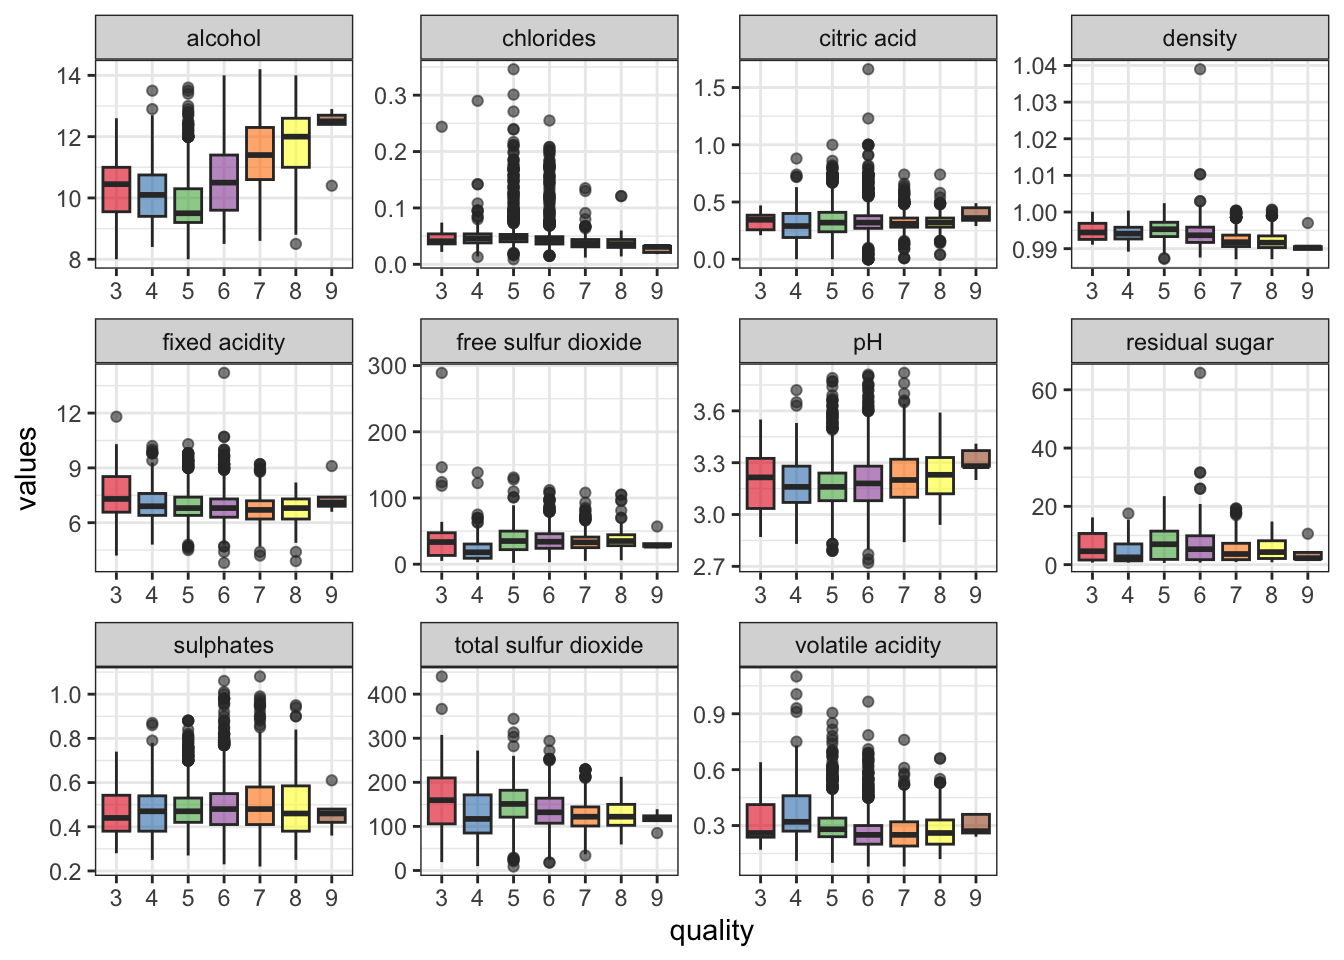
\includegraphics{_main_files/figure-latex/unnamed-chunk-190-1.pdf}

Before doing any kind of preprocessing or normalization, it is imperative to split the data into training and testing to prevent information leak. The \texttt{createDataPartition()} function accepts the \texttt{p\ =} argument which defines the split fraction. Here I use 80/20 split.

\begin{Shaded}
\begin{Highlighting}[]
\FunctionTok{set.seed}\NormalTok{(}\DecValTok{42}\NormalTok{)}
\NormalTok{df }\OtherTok{\textless{}{-}}\NormalTok{ df }\SpecialCharTok{\%\textgreater{}\%} \FunctionTok{mutate}\NormalTok{(}\AttributeTok{quality =} \FunctionTok{paste0}\NormalTok{(}\StringTok{\textquotesingle{}Group\_\textquotesingle{}}\NormalTok{, quality)) }\SpecialCharTok{\%\textgreater{}\%}
  \FunctionTok{mutate}\NormalTok{(}\AttributeTok{quality =} \FunctionTok{factor}\NormalTok{(quality))}

\NormalTok{idx }\OtherTok{\textless{}{-}} \FunctionTok{createDataPartition}\NormalTok{(}\AttributeTok{y =}\NormalTok{ df}\SpecialCharTok{$}\NormalTok{quality, }\AttributeTok{p =}\NormalTok{ .}\DecValTok{8}\NormalTok{,}
                           \AttributeTok{list =} \ConstantTok{FALSE}\NormalTok{, }\AttributeTok{times =} \DecValTok{1}\NormalTok{)}

\NormalTok{df\_train }\OtherTok{\textless{}{-}}\NormalTok{ df[idx,]}
\NormalTok{df\_test }\OtherTok{\textless{}{-}}\NormalTok{ df[}\SpecialCharTok{{-}}\NormalTok{idx,]}
\end{Highlighting}
\end{Shaded}

The \texttt{createDataPartition()} outputs an array of indices which can be used to split the original data.

Going back to the talk of scaling and preprocessing the data: a common procedure is to \texttt{center} and \texttt{scale}, that is - subtract the mean and divide by the standard deviation. If you're familiar with \texttt{scikit-learn} in Python, this is analogous to running \texttt{StandardScaler()}.

\begin{Shaded}
\begin{Highlighting}[]
\NormalTok{preProcObj }\OtherTok{\textless{}{-}} \FunctionTok{preProcess}\NormalTok{(df\_train, }\AttributeTok{method =} \FunctionTok{c}\NormalTok{(}\StringTok{\textquotesingle{}center\textquotesingle{}}\NormalTok{, }\StringTok{\textquotesingle{}scale\textquotesingle{}}\NormalTok{))}
\NormalTok{preProcObj}
\end{Highlighting}
\end{Shaded}

\begin{verbatim}
## Created from 3920 samples and 12 variables
## 
## Pre-processing:
##   - centered (11)
##   - ignored (1)
##   - scaled (11)
\end{verbatim}

Evidently, the \texttt{preProcess()} function recognized the column containing the target labels and ignored it for preprocessing.

Preprocessing is done on the training data and the learned object is applied to both the training and testing data:

\begin{Shaded}
\begin{Highlighting}[]
\NormalTok{df\_train }\OtherTok{\textless{}{-}} \FunctionTok{predict}\NormalTok{(preProcObj, df\_train)}
\NormalTok{df\_test }\OtherTok{\textless{}{-}} \FunctionTok{predict}\NormalTok{(preProcObj, df\_test)}
\end{Highlighting}
\end{Shaded}

Revisiting the features now shows the effect of the preprocessing step:

\begin{Shaded}
\begin{Highlighting}[]
\FunctionTok{summary}\NormalTok{(df\_train }\SpecialCharTok{\%\textgreater{}\%} \FunctionTok{select}\NormalTok{(}\SpecialCharTok{{-}}\NormalTok{quality))}
\end{Highlighting}
\end{Shaded}

\begin{verbatim}
##  fixed acidity      volatile acidity   citric acid     
##  Min.   :-3.63462   Min.   :-1.9812   Min.   :-2.7409  
##  1st Qu.:-0.66724   1st Qu.:-0.6815   1st Qu.:-0.5247  
##  Median :-0.07376   Median :-0.1816   Median :-0.1143  
##  Mean   : 0.00000   Mean   : 0.0000   Mean   : 0.0000  
##  3rd Qu.: 0.63841   3rd Qu.: 0.4182   3rd Qu.: 0.4602  
##  Max.   : 8.70968   Max.   : 7.2663   Max.   :10.8844  
##  residual sugar      chlorides       free sulfur dioxide
##  Min.   :-1.1408   Min.   :-1.6600   Min.   :-1.89691   
##  1st Qu.:-0.9250   1st Qu.:-0.4457   1st Qu.:-0.72325   
##  Median :-0.2384   Median :-0.1309   Median :-0.07773   
##  Mean   : 0.0000   Mean   : 0.0000   Mean   : 0.00000   
##  3rd Qu.: 0.6835   3rd Qu.: 0.1840   3rd Qu.: 0.62647   
##  Max.   :11.6490   Max.   :13.4966   Max.   :14.88647   
##  total sulfur dioxide    density              pH          
##  Min.   :-3.0417      Min.   :-2.2943   Min.   :-2.99893  
##  1st Qu.:-0.6983      1st Qu.:-0.7665   1st Qu.:-0.65873  
##  Median :-0.1065      Median :-0.1122   Median :-0.05697  
##  Mean   : 0.0000      Mean   : 0.0000   Mean   : 0.00000  
##  3rd Qu.: 0.6746      3rd Qu.: 0.7082   3rd Qu.: 0.61166  
##  Max.   : 7.1367      Max.   :14.9270   Max.   : 4.22224  
##    sulphates          alcohol        
##  Min.   :-2.4096   Min.   :-2.05259  
##  1st Qu.:-0.7084   1st Qu.:-0.83024  
##  Median :-0.1711   Median :-0.09683  
##  Mean   : 0.0000   Mean   : 0.00000  
##  3rd Qu.: 0.5452   3rd Qu.: 0.71807  
##  Max.   : 4.4850   Max.   : 2.99978
\end{verbatim}

The scales have been normalized, as evident here:

\begin{Shaded}
\begin{Highlighting}[]
\NormalTok{df\_train }\SpecialCharTok{\%\textgreater{}\%} \FunctionTok{pivot\_longer}\NormalTok{(}\SpecialCharTok{{-}}\NormalTok{quality, }\AttributeTok{names\_to =} \StringTok{\textquotesingle{}feature\textquotesingle{}}\NormalTok{,}
                          \AttributeTok{values\_to =} \StringTok{\textquotesingle{}values\textquotesingle{}}\NormalTok{) }\SpecialCharTok{\%\textgreater{}\%}
  \FunctionTok{ggplot}\NormalTok{(}\FunctionTok{aes}\NormalTok{(}\AttributeTok{x =}\NormalTok{ quality, }\AttributeTok{y =}\NormalTok{ values)) }\SpecialCharTok{+}
  \FunctionTok{geom\_boxplot}\NormalTok{(}\FunctionTok{aes}\NormalTok{(}\AttributeTok{fill =}\NormalTok{ quality), }\AttributeTok{alpha =}\NormalTok{ .}\DecValTok{6}\NormalTok{) }\SpecialCharTok{+}
  \FunctionTok{facet\_wrap}\NormalTok{(}\SpecialCharTok{\textasciitilde{}}\NormalTok{ feature, }\AttributeTok{scales =} \StringTok{\textquotesingle{}free\textquotesingle{}}\NormalTok{) }\SpecialCharTok{+} \FunctionTok{theme\_bw}\NormalTok{() }\SpecialCharTok{+}
  \FunctionTok{theme}\NormalTok{(}\AttributeTok{legend.position =} \StringTok{\textquotesingle{}none\textquotesingle{}}\NormalTok{) }\SpecialCharTok{+} 
  \FunctionTok{scale\_fill\_brewer}\NormalTok{(}\AttributeTok{palette =} \StringTok{\textquotesingle{}Set1\textquotesingle{}}\NormalTok{)}
\end{Highlighting}
\end{Shaded}

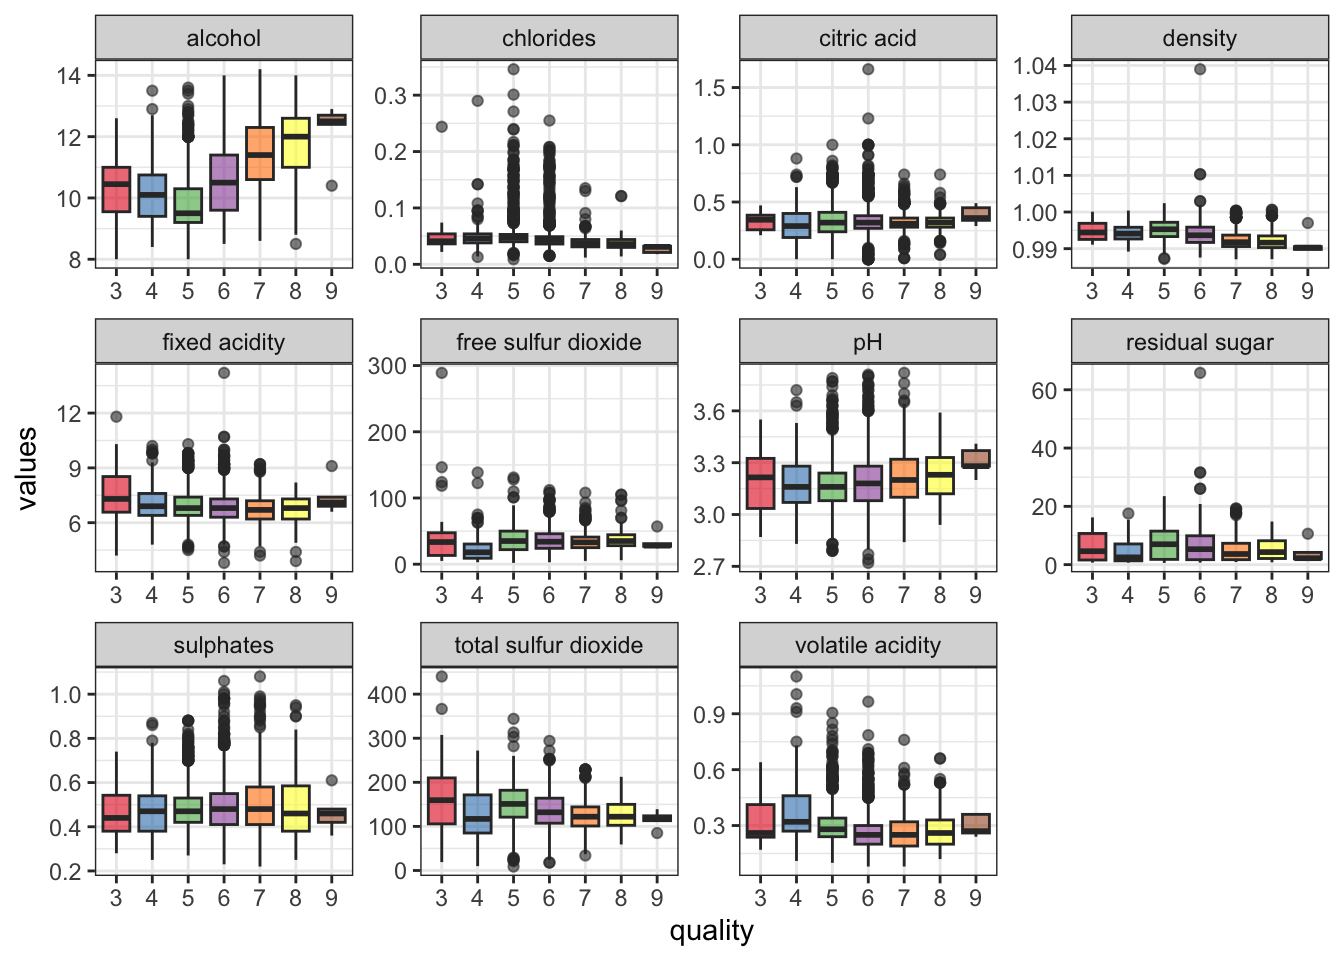
\includegraphics{_main_files/figure-latex/unnamed-chunk-195-1.pdf}

Once we're ready to train the model, an important function is \texttt{trainControl()}. Here, typically we define the sampling method for the model training. I am using \texttt{method\ =\ cv} with \texttt{number\ =\ 5} for k-fold cross-validation with 5 folds. Alternatively, I could use \texttt{method\ =\ repeatedcv} with \texttt{number\ =\ 5} and \texttt{repeats\ =\ 5} for repeated cross-validation with 5 iterations, but for this exercise I will settle with the simple 5-fold cross validation.

\begin{Shaded}
\begin{Highlighting}[]
\NormalTok{tr }\OtherTok{\textless{}{-}} \FunctionTok{trainControl}\NormalTok{(}\AttributeTok{method =} \StringTok{\textquotesingle{}cv\textquotesingle{}}\NormalTok{,}
                   \AttributeTok{number =} \DecValTok{5}\NormalTok{,}
                   \AttributeTok{classProbs =} \ConstantTok{TRUE}\NormalTok{)}

\NormalTok{model }\OtherTok{\textless{}{-}} \FunctionTok{train}\NormalTok{(quality }\SpecialCharTok{\textasciitilde{}}\NormalTok{ ., }\AttributeTok{data =}\NormalTok{ df\_train,}
               \AttributeTok{method =} \StringTok{\textquotesingle{}ranger\textquotesingle{}}\NormalTok{, }\AttributeTok{importance =} \StringTok{\textquotesingle{}impurity\textquotesingle{}}\NormalTok{,}
               \AttributeTok{trControl =}\NormalTok{ tr)}
\end{Highlighting}
\end{Shaded}

Above, I defined \texttt{method\ =\ ranger} within \texttt{train()}, which is a wrapper for training a random forest model. For all available methods for \texttt{train()}, see \texttt{caret}'s documentation \href{https://topepo.github.io/caret/train-models-by-tag.html}{here}. The \texttt{importance\ =\ \textquotesingle{}impurity\textquotesingle{}} asks the model to use the Gini impurity method to rank variable importance. This will be useful later.

Calling the model object summarizes the model's performance on the validation set (i.e., hold-out sets during k-fold cross validation).

\begin{Shaded}
\begin{Highlighting}[]
\NormalTok{model}
\end{Highlighting}
\end{Shaded}

\begin{verbatim}
## Random Forest 
## 
## 3920 samples
##   11 predictor
##    7 classes: 'Group_3', 'Group_4', 'Group_5', 'Group_6', 'Group_7', 'Group_8', 'Group_9' 
## 
## No pre-processing
## Resampling: Cross-Validated (5 fold) 
## Summary of sample sizes: 3136, 3135, 3136, 3137, 3136 
## Resampling results across tuning parameters:
## 
##   mtry  splitrule   Accuracy   Kappa    
##    2    gini        0.6670799  0.4785271
##    2    extratrees  0.6691211  0.4770672
##    6    gini        0.6578979  0.4671397
##    6    extratrees  0.6668264  0.4778833
##   11    gini        0.6571260  0.4668996
##   11    extratrees  0.6647859  0.4756944
## 
## Tuning parameter 'min.node.size' was held constant at
##  a value of 1
## Accuracy was used to select the optimal model using
##  the largest value.
## The final values used for the model were mtry = 2,
##  splitrule = extratrees and min.node.size = 1.
\end{verbatim}

Various hyperparametes were tested and the combination with the highest validation accuracy was chosen:

\begin{Shaded}
\begin{Highlighting}[]
\NormalTok{model}\SpecialCharTok{$}\NormalTok{bestTune}
\end{Highlighting}
\end{Shaded}

\begin{verbatim}
##   mtry  splitrule min.node.size
## 2    2 extratrees             1
\end{verbatim}

The performance on the resamples during the cross validation process can be found here:

\begin{Shaded}
\begin{Highlighting}[]
\NormalTok{model}\SpecialCharTok{$}\NormalTok{resample}
\end{Highlighting}
\end{Shaded}

\begin{verbatim}
##    Accuracy     Kappa Resample
## 1 0.6530612 0.4487323    Fold1
## 2 0.6811224 0.4989916    Fold3
## 3 0.6942675 0.5131632    Fold2
## 4 0.6683673 0.4796363    Fold5
## 5 0.6487867 0.4448126    Fold4
\end{verbatim}

The testing dataset has not been touched at all during model training. For model evaluation, above model is tested on this hold-out set using \texttt{predict()}:

\begin{Shaded}
\begin{Highlighting}[]
\NormalTok{pred }\OtherTok{\textless{}{-}} \FunctionTok{predict}\NormalTok{(model, df\_test)}
\end{Highlighting}
\end{Shaded}

For a clean summary of model evaluation, use \texttt{confusionMatrix()}:

\begin{Shaded}
\begin{Highlighting}[]
\FunctionTok{confusionMatrix}\NormalTok{(}\AttributeTok{data =}\NormalTok{ pred, }\AttributeTok{reference =}\NormalTok{ df\_test}\SpecialCharTok{$}\NormalTok{quality, }
                \AttributeTok{mode =} \StringTok{\textquotesingle{}prec\_recall\textquotesingle{}}\NormalTok{)}
\end{Highlighting}
\end{Shaded}

\begin{verbatim}
## Confusion Matrix and Statistics
## 
##           Reference
## Prediction Group_3 Group_4 Group_5 Group_6 Group_7 Group_8
##    Group_3       0       0       0       0       0       0
##    Group_4       0       7       1       0       0       0
##    Group_5       3      14     217      55       3       1
##    Group_6       1      11      71     360      82      15
##    Group_7       0       0       2      23      90       7
##    Group_8       0       0       0       1       1      12
##    Group_9       0       0       0       0       0       0
##           Reference
## Prediction Group_9
##    Group_3       0
##    Group_4       0
##    Group_5       0
##    Group_6       1
##    Group_7       0
##    Group_8       0
##    Group_9       0
## 
## Overall Statistics
##                                         
##                Accuracy : 0.7014        
##                  95% CI : (0.6717, 0.73)
##     No Information Rate : 0.4489        
##     P-Value [Acc > NIR] : < 2.2e-16     
##                                         
##                   Kappa : 0.533         
##                                         
##  Mcnemar's Test P-Value : NA            
## 
## Statistics by Class:
## 
##                      Class: Group_3 Class: Group_4
## Precision                        NA       0.875000
## Recall                      0.00000       0.218750
## F1                               NA       0.350000
## Prevalence                  0.00409       0.032720
## Detection Rate              0.00000       0.007157
## Detection Prevalence        0.00000       0.008180
## Balanced Accuracy           0.50000       0.608846
##                      Class: Group_5 Class: Group_6
## Precision                    0.7406         0.6654
## Recall                       0.7457         0.8200
## F1                           0.7432         0.7347
## Prevalence                   0.2975         0.4489
## Detection Rate               0.2219         0.3681
## Detection Prevalence         0.2996         0.5532
## Balanced Accuracy            0.8175         0.7421
##                      Class: Group_7 Class: Group_8
## Precision                   0.73770        0.85714
## Recall                      0.51136        0.34286
## F1                          0.60403        0.48980
## Prevalence                  0.17996        0.03579
## Detection Rate              0.09202        0.01227
## Detection Prevalence        0.12474        0.01431
## Balanced Accuracy           0.73573        0.67037
##                      Class: Group_9
## Precision                        NA
## Recall                     0.000000
## F1                               NA
## Prevalence                 0.001022
## Detection Rate             0.000000
## Detection Prevalence       0.000000
## Balanced Accuracy          0.500000
\end{verbatim}

Certain models such as the random forest have built-in feature importance. During model training, I defined \texttt{importance\ =\ \textquotesingle{}impurity\textquotesingle{}}, which means that the feature importance is calculated using the mean decrease in impurity after permutation of a given feature. Accessing this information is useful when we want to know which variables have the greatest influence on model performance and conversely, which ones have the least.

\begin{Shaded}
\begin{Highlighting}[]
\FunctionTok{varImp}\NormalTok{(model)}\SpecialCharTok{$}\NormalTok{importance}
\end{Highlighting}
\end{Shaded}

\begin{verbatim}
##                           Overall
## `fixed acidity`          0.000000
## `volatile acidity`      35.165026
## `citric acid`            8.761852
## `residual sugar`        11.579565
## chlorides                4.090038
## `free sulfur dioxide`   14.832990
## `total sulfur dioxide`  12.411664
## density                 38.947736
## pH                       7.484357
## sulphates                2.801255
## alcohol                100.000000
\end{verbatim}

The variable importance score is automatically scaled so that the highest score is set to 100. This can be turned off using \texttt{scale\ =\ FALSE} within \texttt{varImp()}.

A quick visualization of variable importance is useful:

\begin{Shaded}
\begin{Highlighting}[]
\NormalTok{df\_imp }\OtherTok{\textless{}{-}} \FunctionTok{varImp}\NormalTok{(model)}\SpecialCharTok{$}\NormalTok{importance }\SpecialCharTok{\%\textgreater{}\%} 
  \FunctionTok{rownames\_to\_column}\NormalTok{(}\AttributeTok{var =} \StringTok{\textquotesingle{}Var\textquotesingle{}}\NormalTok{) }\SpecialCharTok{\%\textgreater{}\%}
  \FunctionTok{as\_tibble}\NormalTok{() }\SpecialCharTok{\%\textgreater{}\%} \FunctionTok{arrange}\NormalTok{(}\FunctionTok{desc}\NormalTok{(Overall))}

\FunctionTok{ggplot}\NormalTok{(df\_imp, }\FunctionTok{aes}\NormalTok{(}\AttributeTok{x =} \FunctionTok{reorder}\NormalTok{(Var, Overall), }\AttributeTok{y =}\NormalTok{ Overall)) }\SpecialCharTok{+} 
  \FunctionTok{geom\_point}\NormalTok{(}\AttributeTok{stat =} \StringTok{\textquotesingle{}identity\textquotesingle{}}\NormalTok{, }\AttributeTok{color =} \StringTok{\textquotesingle{}red\textquotesingle{}}\NormalTok{) }\SpecialCharTok{+} 
  \FunctionTok{geom\_segment}\NormalTok{(}\FunctionTok{aes}\NormalTok{(}\AttributeTok{x =} \FunctionTok{reorder}\NormalTok{(Var, Overall), }
                   \AttributeTok{xend =} \FunctionTok{reorder}\NormalTok{(Var, Overall),}
                   \AttributeTok{y =} \DecValTok{0}\NormalTok{,}
                   \AttributeTok{yend =}\NormalTok{ Overall)) }\SpecialCharTok{+} 
  \FunctionTok{theme\_classic}\NormalTok{() }\SpecialCharTok{+} \FunctionTok{coord\_flip}\NormalTok{() }\SpecialCharTok{+} \FunctionTok{xlab}\NormalTok{(}\StringTok{\textquotesingle{}\textquotesingle{}}\NormalTok{) }\SpecialCharTok{+} \FunctionTok{ylab}\NormalTok{(}\StringTok{\textquotesingle{}Var. Imp.\textquotesingle{}}\NormalTok{) }\SpecialCharTok{+}
  \FunctionTok{theme}\NormalTok{(}\AttributeTok{text =} \FunctionTok{element\_text}\NormalTok{(}\AttributeTok{size =} \DecValTok{14}\NormalTok{))}
\end{Highlighting}
\end{Shaded}

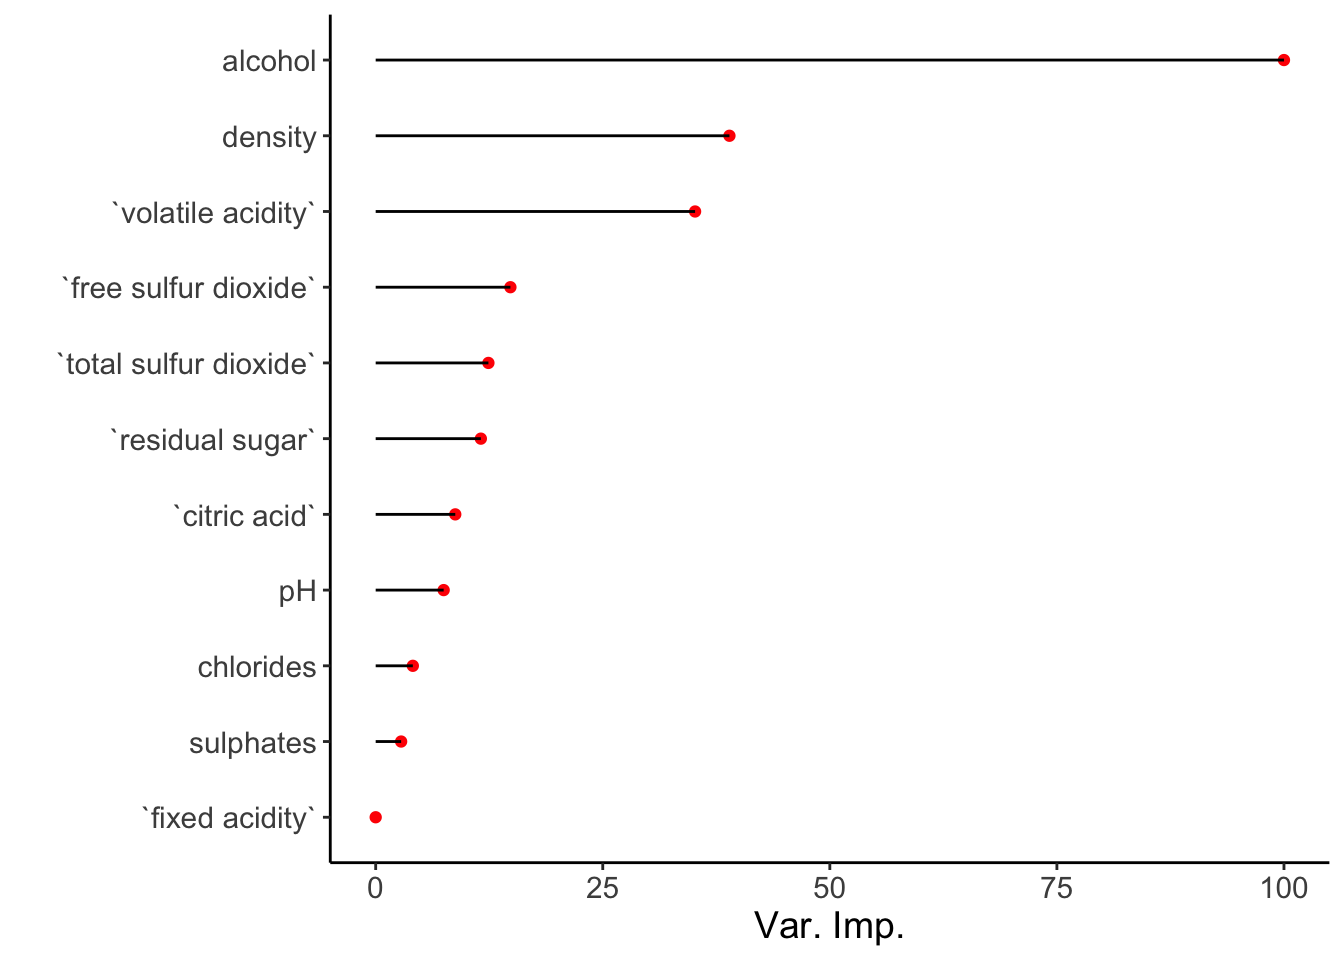
\includegraphics{_main_files/figure-latex/unnamed-chunk-203-1.pdf}

\hypertarget{feature-selection-using-univariate-filters}{%
\section{Feature selection using univariate filters}\label{feature-selection-using-univariate-filters}}

When the dataset is considerably larger, the number of \emph{n} features may grow extremely large. In these scenarios, it may be advisable to reduce the number of features to save computation time but also to reduce model complexity.

Of course, dimensionality reduction is possible, though this transforms the data and the original meaning of the features is lost. An alternative method is \emph{feature selection} - selecting important features and discarding unimportant ones. This relates specifically to the concept of feature importance in the previous section.

\texttt{caret} offers a simple way to rank features when built-in feature importance measures are not available. This is by using univariate filters, which are essentially fitting \emph{n} individual models (where \emph{n} is the number of features) against the target label and ranking them based on their statistical significance.

\texttt{anoveScores()} is used for classification models and fits an ANOVA for each feature against the label. The null hypothesis here assumes the mean values for each feature is equal for all labels. \texttt{gamScores()} is used for regression models and uses a generalized additive model to look for functional relationships between the features and the label. In both cases, each feature in the predictor set is passed individually.

For this part I will use the \texttt{Sonar} dataset from \texttt{mlbench}.

\begin{Shaded}
\begin{Highlighting}[]
\FunctionTok{library}\NormalTok{(mlbench)}
\FunctionTok{data}\NormalTok{(Sonar)}
\NormalTok{Sonar }\OtherTok{\textless{}{-}} \FunctionTok{as\_tibble}\NormalTok{(Sonar)}
\NormalTok{Sonar}
\end{Highlighting}
\end{Shaded}

\begin{verbatim}
## # A tibble: 208 x 61
##        V1     V2     V3     V4     V5     V6     V7     V8
##     <dbl>  <dbl>  <dbl>  <dbl>  <dbl>  <dbl>  <dbl>  <dbl>
##  1 0.02   0.0371 0.0428 0.0207 0.0954 0.0986 0.154  0.160 
##  2 0.0453 0.0523 0.0843 0.0689 0.118  0.258  0.216  0.348 
##  3 0.0262 0.0582 0.110  0.108  0.0974 0.228  0.243  0.377 
##  4 0.01   0.0171 0.0623 0.0205 0.0205 0.0368 0.110  0.128 
##  5 0.0762 0.0666 0.0481 0.0394 0.059  0.0649 0.121  0.247 
##  6 0.0286 0.0453 0.0277 0.0174 0.0384 0.099  0.120  0.183 
##  7 0.0317 0.0956 0.132  0.141  0.167  0.171  0.0731 0.140 
##  8 0.0519 0.0548 0.0842 0.0319 0.116  0.0922 0.103  0.0613
##  9 0.0223 0.0375 0.0484 0.0475 0.0647 0.0591 0.0753 0.0098
## 10 0.0164 0.0173 0.0347 0.007  0.0187 0.0671 0.106  0.0697
## # ... with 198 more rows, and 53 more variables: V9 <dbl>,
## #   V10 <dbl>, V11 <dbl>, V12 <dbl>, V13 <dbl>, V14 <dbl>,
## #   V15 <dbl>, V16 <dbl>, V17 <dbl>, V18 <dbl>, V19 <dbl>,
## #   V20 <dbl>, V21 <dbl>, V22 <dbl>, V23 <dbl>, V24 <dbl>,
## #   V25 <dbl>, V26 <dbl>, V27 <dbl>, V28 <dbl>, V29 <dbl>,
## #   V30 <dbl>, V31 <dbl>, V32 <dbl>, V33 <dbl>, V34 <dbl>,
## #   V35 <dbl>, V36 <dbl>, V37 <dbl>, V38 <dbl>, ...
\end{verbatim}

The target labels in \texttt{Sonar} has two classes:

\begin{Shaded}
\begin{Highlighting}[]
\NormalTok{Sonar}\SpecialCharTok{$}\NormalTok{Class }\SpecialCharTok{\%\textgreater{}\%} \FunctionTok{str}\NormalTok{()}
\end{Highlighting}
\end{Shaded}

\begin{verbatim}
##  Factor w/ 2 levels "M","R": 2 2 2 2 2 2 2 2 2 2 ...
\end{verbatim}

Since this is a classification task, I will use \texttt{anovaScores()} to output a score for each feature.

\begin{Shaded}
\begin{Highlighting}[]
\NormalTok{fit\_anova }\OtherTok{\textless{}{-}} \ControlFlowTok{function}\NormalTok{(x, y) \{}
\NormalTok{    anova\_res }\OtherTok{\textless{}{-}} \FunctionTok{apply}\NormalTok{(x, }\DecValTok{2}\NormalTok{, }\ControlFlowTok{function}\NormalTok{(f) \{}\FunctionTok{anovaScores}\NormalTok{(f, y)\})}
    \FunctionTok{return}\NormalTok{(anova\_res)}
\NormalTok{\}}

\NormalTok{aov\_res }\OtherTok{\textless{}{-}} \FunctionTok{fit\_anova}\NormalTok{(}\AttributeTok{x =} \FunctionTok{select}\NormalTok{(Sonar, }\SpecialCharTok{{-}}\NormalTok{Class), }
                     \AttributeTok{y =}\NormalTok{ Sonar}\SpecialCharTok{$}\NormalTok{Class)}

\NormalTok{aov\_res }\OtherTok{\textless{}{-}} \FunctionTok{as.data.frame}\NormalTok{(aov\_res)}
\FunctionTok{head}\NormalTok{(aov\_res)}
\end{Highlighting}
\end{Shaded}

\begin{verbatim}
##         aov_res
## V1 0.0000719490
## V2 0.0007779402
## V3 0.0054167746
## V4 0.0002607819
## V5 0.0012544689
## V6 0.0567376774
\end{verbatim}

The output for each feature is the p-value for the whole model F-test. These can be ranked to find the features with the greatest degree of relationship with the target labels:

\begin{Shaded}
\begin{Highlighting}[]
\NormalTok{aov\_res }\OtherTok{\textless{}{-}}\NormalTok{ aov\_res }\SpecialCharTok{\%\textgreater{}\%} \FunctionTok{rownames\_to\_column}\NormalTok{(}\AttributeTok{var =} \StringTok{\textquotesingle{}Var\textquotesingle{}}\NormalTok{) }\SpecialCharTok{\%\textgreater{}\%}
  \FunctionTok{as\_tibble}\NormalTok{() }\SpecialCharTok{\%\textgreater{}\%} \FunctionTok{rename}\NormalTok{(}\AttributeTok{pVal =}\NormalTok{ aov\_res) }\SpecialCharTok{\%\textgreater{}\%} \FunctionTok{arrange}\NormalTok{(aov\_res)}

\NormalTok{aov\_res}
\end{Highlighting}
\end{Shaded}

\begin{verbatim}
## # A tibble: 60 x 2
##    Var       pVal
##    <chr>    <dbl>
##  1 V11   6.59e-11
##  2 V12   4.64e- 9
##  3 V49   1.96e- 7
##  4 V10   4.60e- 7
##  5 V45   5.30e- 7
##  6 V48   1.19e- 6
##  7 V9    2.20e- 6
##  8 V13   4.22e- 6
##  9 V46   7.16e- 6
## 10 V47   9.49e- 6
## # ... with 50 more rows
\end{verbatim}

\hypertarget{feature-selection-using-recursive-feature-elimination}{%
\section{Feature selection using recursive feature elimination}\label{feature-selection-using-recursive-feature-elimination}}

An alternative method for feature selection is recursive feature elimination (RFE). RFE is a wrapper method that uses another model to rank features based on variable importance. This model does not have to be the same model used in the downstream model prediction task.

The feature importance ranking method depends which model the RFE wrapper uses. Tree models such as the random forest, as previous mentioned, can use impurity scores or mean accuracy decrease to calculate this.

The \texttt{rfeControl()} function specifies the RFE model as well as the resampling method. Then \texttt{rfe()} runs the algorithm to identify important features as well as the model accuracy as the RFE recursively removes the less important features and trains the model.

\begin{Shaded}
\begin{Highlighting}[]
\NormalTok{rfec }\OtherTok{\textless{}{-}} \FunctionTok{rfeControl}\NormalTok{(}\AttributeTok{functions =}\NormalTok{ rfFuncs, }\AttributeTok{method =} \StringTok{\textquotesingle{}cv\textquotesingle{}}\NormalTok{,}
                  \AttributeTok{number =} \DecValTok{5}\NormalTok{)}

\NormalTok{rfeObj }\OtherTok{\textless{}{-}} \FunctionTok{rfe}\NormalTok{(}\AttributeTok{x =} \FunctionTok{select}\NormalTok{(Sonar, }\SpecialCharTok{{-}}\NormalTok{Class), }\AttributeTok{y =}\NormalTok{ Sonar}\SpecialCharTok{$}\NormalTok{Class,}
              \AttributeTok{rfeControl =}\NormalTok{ rfec)}
\end{Highlighting}
\end{Shaded}

Calling the output shows that the top 5 most important features show overlap with the result from \texttt{anovaScores()} from the previous section, which is good. It also shows that keeping the original 60 features here shows the best model accuracy, which is fine. This won't always be the case with increasing number of dimensions in the data.

\begin{Shaded}
\begin{Highlighting}[]
\NormalTok{rfeObj}
\end{Highlighting}
\end{Shaded}

\begin{verbatim}
## 
## Recursive feature selection
## 
## Outer resampling method: Cross-Validated (5 fold) 
## 
## Resampling performance over subset size:
## 
##  Variables Accuracy  Kappa AccuracySD KappaSD Selected
##          4   0.7212 0.4398    0.05514 0.11064         
##          8   0.7308 0.4557    0.04581 0.09426         
##         16   0.7790 0.5539    0.05389 0.10782         
##         60   0.8176 0.6290    0.06359 0.12886        *
## 
## The top 5 variables (out of 60):
##    V11, V12, V9, V10, V48
\end{verbatim}

The fitted model and its performance can be retrieved as such:

\begin{Shaded}
\begin{Highlighting}[]
\NormalTok{rfeObj}\SpecialCharTok{$}\NormalTok{fit}
\end{Highlighting}
\end{Shaded}

\begin{verbatim}
## 
## Call:
##  randomForest(x = x, y = y, importance = TRUE) 
##                Type of random forest: classification
##                      Number of trees: 500
## No. of variables tried at each split: 7
## 
##         OOB estimate of  error rate: 15.87%
## Confusion matrix:
##     M  R class.error
## M 101 10  0.09009009
## R  23 74  0.23711340
\end{verbatim}

The ranking of the features can be retreived here, which is useful if we were to select the first few and subset our original dataset:

\begin{Shaded}
\begin{Highlighting}[]
\NormalTok{rfeObj}\SpecialCharTok{$}\NormalTok{optVariables}
\end{Highlighting}
\end{Shaded}

\begin{verbatim}
##  [1] "V11" "V12" "V9"  "V10" "V48" "V47" "V36" "V49" "V28"
## [10] "V45" "V37" "V21" "V46" "V16" "V13" "V17" "V51" "V27"
## [19] "V4"  "V15" "V20" "V18" "V52" "V5"  "V44" "V23" "V1" 
## [28] "V31" "V43" "V26" "V22" "V35" "V19" "V30" "V14" "V8" 
## [37] "V39" "V34" "V32" "V24" "V54" "V42" "V29" "V59" "V55"
## [46] "V25" "V2"  "V6"  "V41" "V58" "V38" "V3"  "V33" "V40"
## [55] "V50" "V7"  "V53" "V57" "V60" "V56"
\end{verbatim}

Calling \texttt{ggplot()} on the RFE result provides a visual look:

\begin{Shaded}
\begin{Highlighting}[]
\FunctionTok{ggplot}\NormalTok{(rfeObj) }\SpecialCharTok{+} \FunctionTok{theme\_bw}\NormalTok{()}
\end{Highlighting}
\end{Shaded}

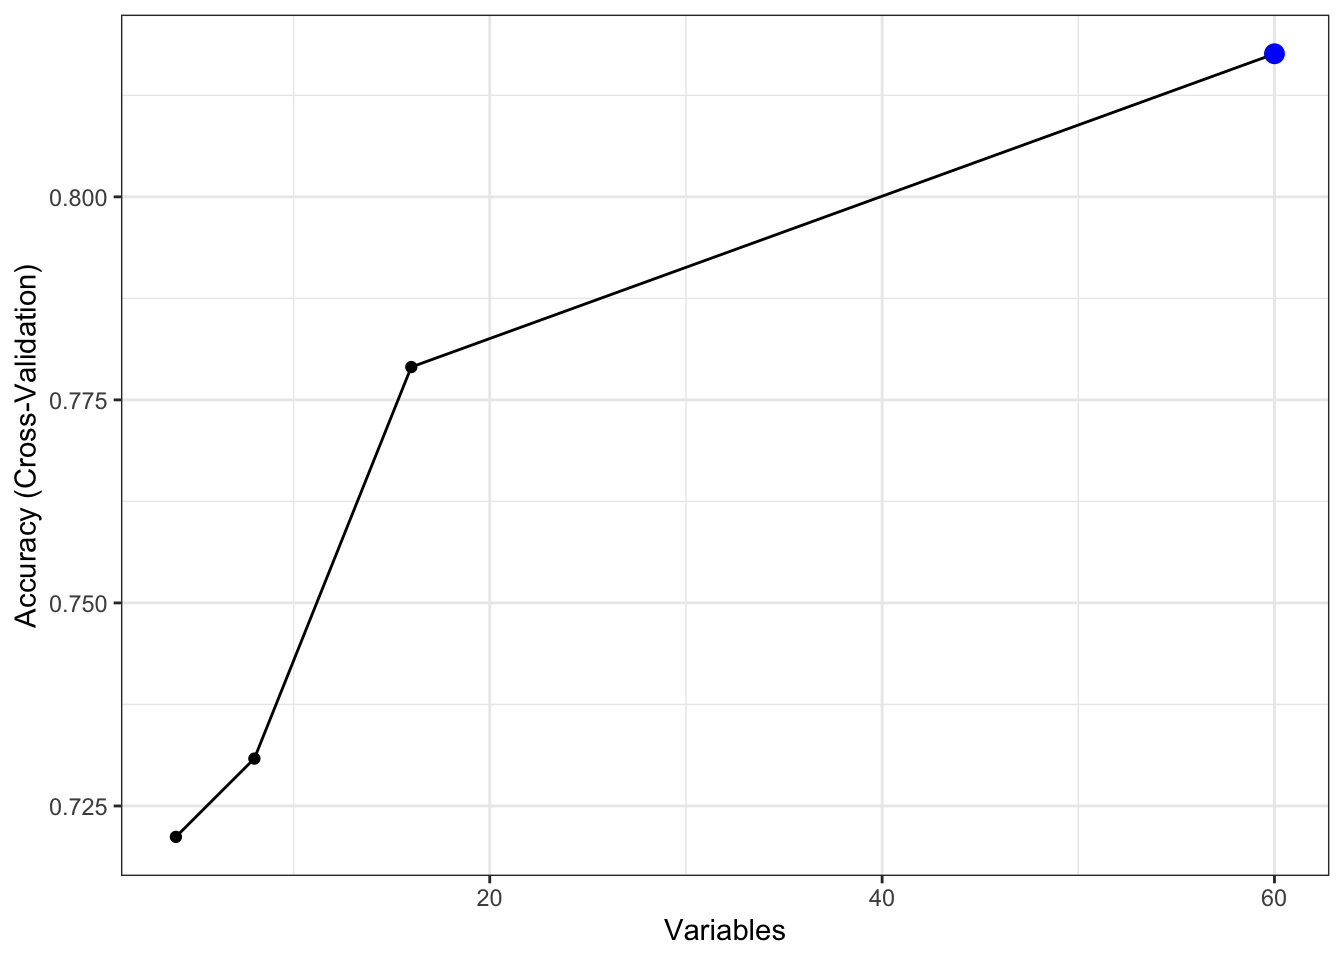
\includegraphics{_main_files/figure-latex/unnamed-chunk-212-1.pdf}

\hypertarget{hyperparameter-tuning}{%
\section{Hyperparameter tuning}\label{hyperparameter-tuning}}

Previously when we trained the random forest model using \texttt{train()}, it automatically deduced the optimal values for the model hyperparameters. Under the hood, \texttt{train()} ran a grid search to find these values, but we can define our own grid as well.

Hyperparameter tuning should of course be done on the training set, so I will use the \texttt{Sonar} dataset to arrive at the training and testing sets:

\begin{Shaded}
\begin{Highlighting}[]
\NormalTok{idx }\OtherTok{\textless{}{-}} \FunctionTok{createDataPartition}\NormalTok{(}\AttributeTok{y =}\NormalTok{ Sonar}\SpecialCharTok{$}\NormalTok{Class, }\AttributeTok{p =}\NormalTok{ .}\DecValTok{8}\NormalTok{,}
                           \AttributeTok{list =} \ConstantTok{FALSE}\NormalTok{, }\AttributeTok{times =} \DecValTok{1}\NormalTok{)}

\NormalTok{df\_train }\OtherTok{\textless{}{-}}\NormalTok{ Sonar[idx,]}
\NormalTok{df\_test }\OtherTok{\textless{}{-}}\NormalTok{ Sonar[}\SpecialCharTok{{-}}\NormalTok{idx,]}

\NormalTok{preProcObj }\OtherTok{\textless{}{-}} \FunctionTok{preProcess}\NormalTok{(df\_train, }\AttributeTok{method =} \FunctionTok{c}\NormalTok{(}\StringTok{\textquotesingle{}center\textquotesingle{}}\NormalTok{, }\StringTok{\textquotesingle{}scale\textquotesingle{}}\NormalTok{))}
\NormalTok{df\_train }\OtherTok{\textless{}{-}} \FunctionTok{predict}\NormalTok{(preProcObj, df\_train)}
\NormalTok{df\_test }\OtherTok{\textless{}{-}} \FunctionTok{predict}\NormalTok{(preProcObj, df\_test)}
\end{Highlighting}
\end{Shaded}

For the random forest model, I define the possible values for the three hyperparameters as such, and then train by providing an input for \texttt{tuneGrid\ =}.

\begin{Shaded}
\begin{Highlighting}[]
\NormalTok{rf\_grid }\OtherTok{\textless{}{-}} \FunctionTok{expand.grid}\NormalTok{(}\AttributeTok{mtry =} \FunctionTok{c}\NormalTok{(}\DecValTok{2}\NormalTok{, }\DecValTok{4}\NormalTok{, }\DecValTok{8}\NormalTok{, }\DecValTok{10}\NormalTok{), }
                       \AttributeTok{splitrule =} \FunctionTok{c}\NormalTok{(}\StringTok{"gini"}\NormalTok{, }\StringTok{"extratrees"}\NormalTok{), }
                       \AttributeTok{min.node.size =} \FunctionTok{c}\NormalTok{(}\DecValTok{1}\NormalTok{, }\DecValTok{3}\NormalTok{, }\DecValTok{5}\NormalTok{))}

\NormalTok{model\_rf }\OtherTok{\textless{}{-}} \FunctionTok{train}\NormalTok{(Class }\SpecialCharTok{\textasciitilde{}}\NormalTok{ ., }\AttributeTok{data =}\NormalTok{ df\_train, }\AttributeTok{method =} \StringTok{\textquotesingle{}ranger\textquotesingle{}}\NormalTok{,}
                    \AttributeTok{importance =} \StringTok{\textquotesingle{}impurity\textquotesingle{}}\NormalTok{, }\AttributeTok{trControl =}\NormalTok{ tr,}
                    \AttributeTok{tuneGrid =}\NormalTok{ rf\_grid)}
\end{Highlighting}
\end{Shaded}

Calling the model then shows the model performance (with the specified resampling method) for each combination of the grid search:

\begin{Shaded}
\begin{Highlighting}[]
\NormalTok{model\_rf}
\end{Highlighting}
\end{Shaded}

\begin{verbatim}
## Random Forest 
## 
## 167 samples
##  60 predictor
##   2 classes: 'M', 'R' 
## 
## No pre-processing
## Resampling: Cross-Validated (5 fold) 
## Summary of sample sizes: 133, 133, 134, 133, 135 
## Resampling results across tuning parameters:
## 
##   mtry  splitrule   min.node.size  Accuracy   Kappa    
##    2    gini        1              0.8151181  0.6228532
##    2    gini        3              0.8327540  0.6590288
##    2    gini        5              0.8090463  0.6096000
##    2    extratrees  1              0.8207999  0.6350424
##    2    extratrees  3              0.8211676  0.6358619
##    2    extratrees  5              0.8022504  0.5957834
##    4    gini        1              0.8329434  0.6587746
##    4    gini        3              0.8210004  0.6353605
##    4    gini        5              0.8268828  0.6467128
##    4    extratrees  1              0.8206217  0.6332840
##    4    extratrees  3              0.8325758  0.6576618
##    4    extratrees  5              0.8450646  0.6844312
##    8    gini        1              0.8208222  0.6363709
##    8    gini        3              0.8268828  0.6495138
##    8    gini        5              0.8208222  0.6357195
##    8    extratrees  1              0.8445187  0.6823220
##    8    extratrees  3              0.8388146  0.6720493
##    8    extratrees  5              0.8272282  0.6488559
##   10    gini        1              0.8329434  0.6599363
##   10    gini        3              0.8388369  0.6717421
##   10    gini        5              0.8267045  0.6480589
##   10    extratrees  1              0.8206217  0.6339633
##   10    extratrees  3              0.8441511  0.6816926
##   10    extratrees  5              0.8265040  0.6457295
## 
## Accuracy was used to select the optimal model using
##  the largest value.
## The final values used for the model were mtry = 4,
##  splitrule = extratrees and min.node.size = 5.
\end{verbatim}

As before, the best set of hyperparameters can be retrieved:

\begin{Shaded}
\begin{Highlighting}[]
\NormalTok{model\_rf}\SpecialCharTok{$}\NormalTok{bestTune}
\end{Highlighting}
\end{Shaded}

\begin{verbatim}
##    mtry  splitrule min.node.size
## 12    4 extratrees             5
\end{verbatim}

Instead of a predefined grid search, we can do a randomized search instead. This can be done by setting \texttt{search\ =\ \textquotesingle{}random\textquotesingle{}} within \texttt{trainControl()} first and then specifying \texttt{tuneLength\ =} in \texttt{train()}.

Since we've only used random forest models so far, here I will do a similar grid search but using a support vector machine (SVM) with the radial basis function kernel instead:

\begin{Shaded}
\begin{Highlighting}[]
\NormalTok{tr\_svm }\OtherTok{\textless{}{-}} \FunctionTok{trainControl}\NormalTok{(}\AttributeTok{method =} \StringTok{\textquotesingle{}cv\textquotesingle{}}\NormalTok{,}
                   \AttributeTok{number =} \DecValTok{5}\NormalTok{,}
                   \AttributeTok{classProbs =} \ConstantTok{TRUE}\NormalTok{,}
                   \AttributeTok{search =} \StringTok{\textquotesingle{}random\textquotesingle{}}\NormalTok{)}

\NormalTok{model\_svm }\OtherTok{\textless{}{-}} \FunctionTok{train}\NormalTok{(Class }\SpecialCharTok{\textasciitilde{}}\NormalTok{ ., }\AttributeTok{data =}\NormalTok{ df\_train, }
                   \AttributeTok{method =} \StringTok{\textquotesingle{}svmRadial\textquotesingle{}}\NormalTok{,}
                   \AttributeTok{trControl =}\NormalTok{ tr\_svm, }
                   \AttributeTok{tunelength =} \DecValTok{8}\NormalTok{)}
\end{Highlighting}
\end{Shaded}

Calling the model shows the best combination for \texttt{C} (cost) and \texttt{sigma} based on the model accuracy:

\begin{Shaded}
\begin{Highlighting}[]
\NormalTok{model\_svm}
\end{Highlighting}
\end{Shaded}

\begin{verbatim}
## Support Vector Machines with Radial Basis Function Kernel 
## 
## 167 samples
##  60 predictor
##   2 classes: 'M', 'R' 
## 
## No pre-processing
## Resampling: Cross-Validated (5 fold) 
## Summary of sample sizes: 133, 133, 133, 134, 135 
## Resampling results across tuning parameters:
## 
##   sigma        C           Accuracy   Kappa    
##   0.002678978   58.142065  0.7708445  0.5357187
##   0.024781262  563.129570  0.8680481  0.7316302
##   0.033519260    2.093291  0.8564617  0.7081256
## 
## Accuracy was used to select the optimal model using
##  the largest value.
## The final values used for the model were sigma =
##  0.02478126 and C = 563.1296.
\end{verbatim}

\hypertarget{roc-and-precision-recall-curves}{%
\section{ROC and precision-recall curves}\label{roc-and-precision-recall-curves}}

A nice way to visualize model evaluation is by using ROC curves, which uses metrics that were already calculated previously - precision and recall.

For this I will generate predictions for the random forest model using \texttt{Sonar}. Setting \texttt{type\ =\ \textquotesingle{}prob\textquotesingle{}} yields probabilities for each label classification instead of the label itself:

\begin{Shaded}
\begin{Highlighting}[]
\NormalTok{pred }\OtherTok{\textless{}{-}} \FunctionTok{predict}\NormalTok{(model\_rf, df\_test, }\AttributeTok{type =} \StringTok{\textquotesingle{}prob\textquotesingle{}}\NormalTok{)}
\FunctionTok{head}\NormalTok{(pred)}
\end{Highlighting}
\end{Shaded}

\begin{verbatim}
##           M         R
## 1 0.5870667 0.4129333
## 2 0.6210333 0.3789667
## 3 0.4531667 0.5468333
## 4 0.2409667 0.7590333
## 5 0.6803667 0.3196333
## 6 0.1867333 0.8132667
\end{verbatim}

The package \texttt{MLeval} can be used to generate ROC curves as such; here we achieve the ROC area under the curve of 0.96.

\begin{Shaded}
\begin{Highlighting}[]
\FunctionTok{library}\NormalTok{(MLeval)}
\end{Highlighting}
\end{Shaded}

\begin{verbatim}
## 
## Attaching package: 'MLeval'
\end{verbatim}

\begin{verbatim}
## The following object is masked _by_ '.GlobalEnv':
## 
##     Sonar
\end{verbatim}

\begin{Shaded}
\begin{Highlighting}[]
\NormalTok{roc\_rf }\OtherTok{\textless{}{-}} \FunctionTok{evalm}\NormalTok{(}\FunctionTok{data.frame}\NormalTok{(pred, df\_test}\SpecialCharTok{$}\NormalTok{Class, }\AttributeTok{Group =} \StringTok{\textquotesingle{}RF\textquotesingle{}}\NormalTok{), }
                \AttributeTok{showplots =} \ConstantTok{FALSE}\NormalTok{, }\AttributeTok{silent =} \ConstantTok{TRUE}\NormalTok{)}
\NormalTok{roc\_rf}\SpecialCharTok{$}\NormalTok{roc}
\end{Highlighting}
\end{Shaded}

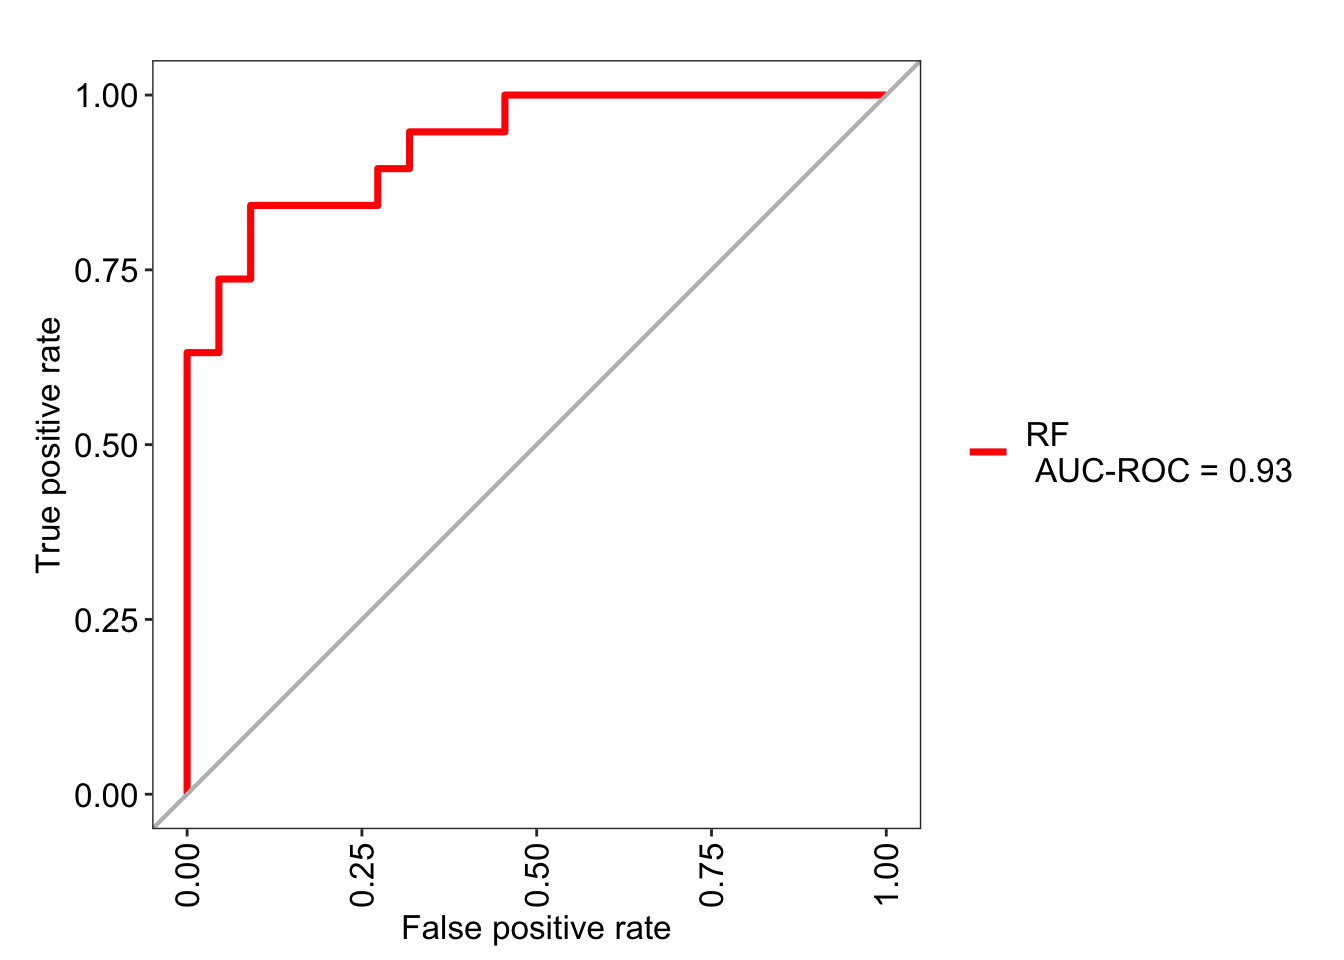
\includegraphics{_main_files/figure-latex/unnamed-chunk-220-1.pdf}

Similarly, a precision-recall curve can also be visualized. This curve shows the tradeoff between the two metrics for each threshold.

\begin{Shaded}
\begin{Highlighting}[]
\NormalTok{roc\_rf}\SpecialCharTok{$}\NormalTok{proc}
\end{Highlighting}
\end{Shaded}

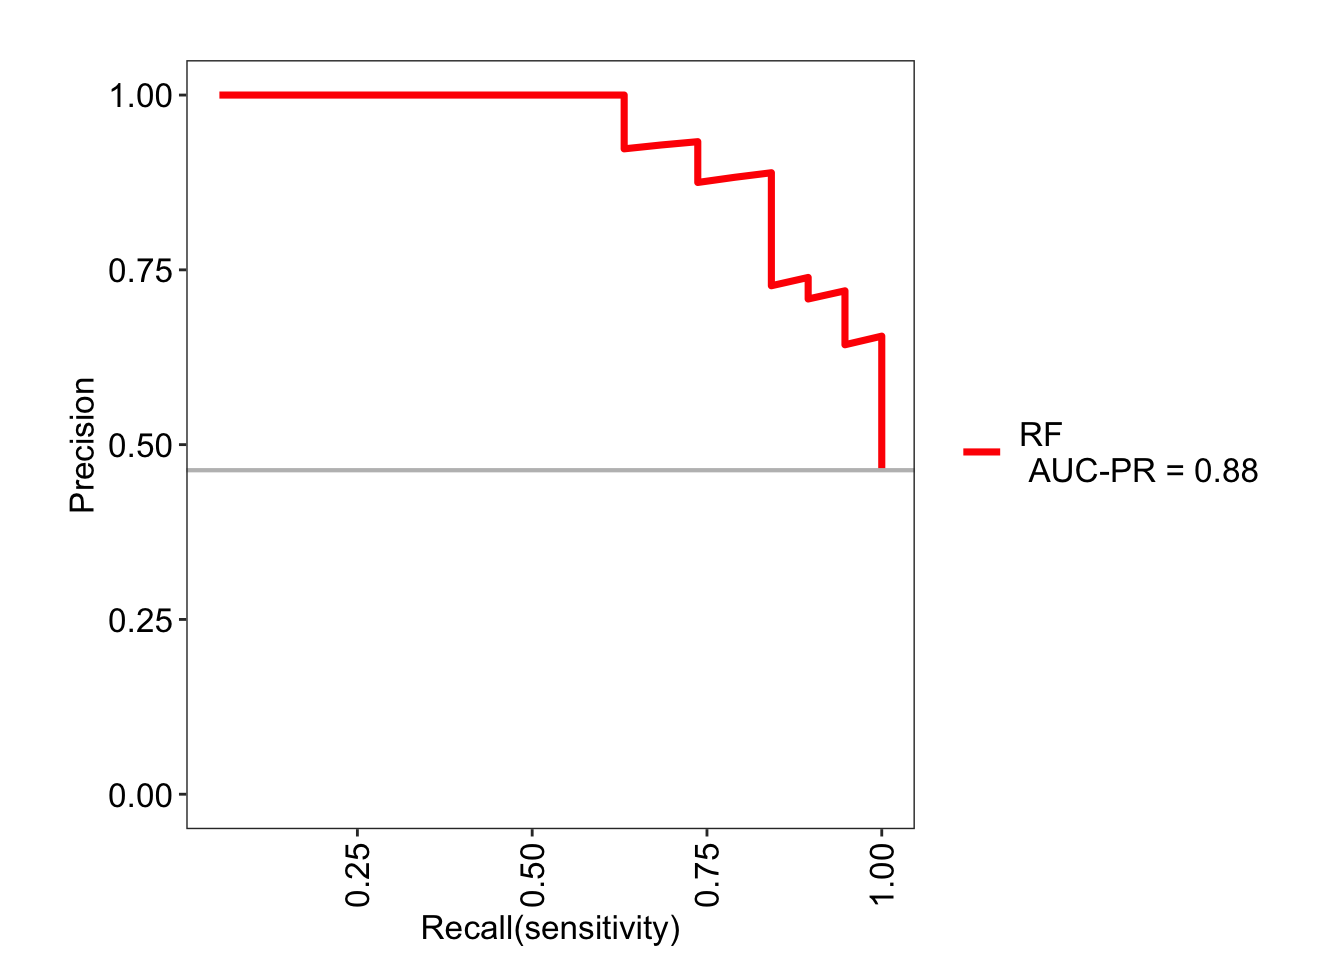
\includegraphics{_main_files/figure-latex/unnamed-chunk-221-1.pdf}

The values can be retrieved here:

\begin{Shaded}
\begin{Highlighting}[]
\NormalTok{roc\_rf}\SpecialCharTok{$}\NormalTok{optres}
\end{Highlighting}
\end{Shaded}

\begin{verbatim}
## $RF
##               Score        CI
## SENS          0.842 0.62-0.94
## SPEC          0.909 0.72-0.97
## MCC           0.755      <NA>
## Informedness  0.751      <NA>
## PREC          0.889 0.67-0.97
## NPV           0.870 0.68-0.95
## FPR           0.091      <NA>
## F1            0.865      <NA>
## TP           16.000      <NA>
## FP            2.000      <NA>
## TN           20.000      <NA>
## FN            3.000      <NA>
## AUC-ROC       0.930 0.84-1.02
## AUC-PR        0.880      <NA>
## AUC-PRG       0.610      <NA>
\end{verbatim}

For completeness I will make these figures for the SVM model as well:

\begin{Shaded}
\begin{Highlighting}[]
\NormalTok{pred2 }\OtherTok{\textless{}{-}} \FunctionTok{predict}\NormalTok{(model\_svm, df\_test, }\AttributeTok{type =} \StringTok{\textquotesingle{}prob\textquotesingle{}}\NormalTok{)}
\end{Highlighting}
\end{Shaded}

\begin{Shaded}
\begin{Highlighting}[]
\NormalTok{roc\_svm }\OtherTok{\textless{}{-}} \FunctionTok{evalm}\NormalTok{(}\FunctionTok{data.frame}\NormalTok{(pred2, df\_test}\SpecialCharTok{$}\NormalTok{Class, }\AttributeTok{Group =} \StringTok{\textquotesingle{}SVM\textquotesingle{}}\NormalTok{), }
                \AttributeTok{showplots =} \ConstantTok{FALSE}\NormalTok{, }\AttributeTok{silent =} \ConstantTok{TRUE}\NormalTok{)}
\NormalTok{roc\_svm}\SpecialCharTok{$}\NormalTok{roc}
\end{Highlighting}
\end{Shaded}

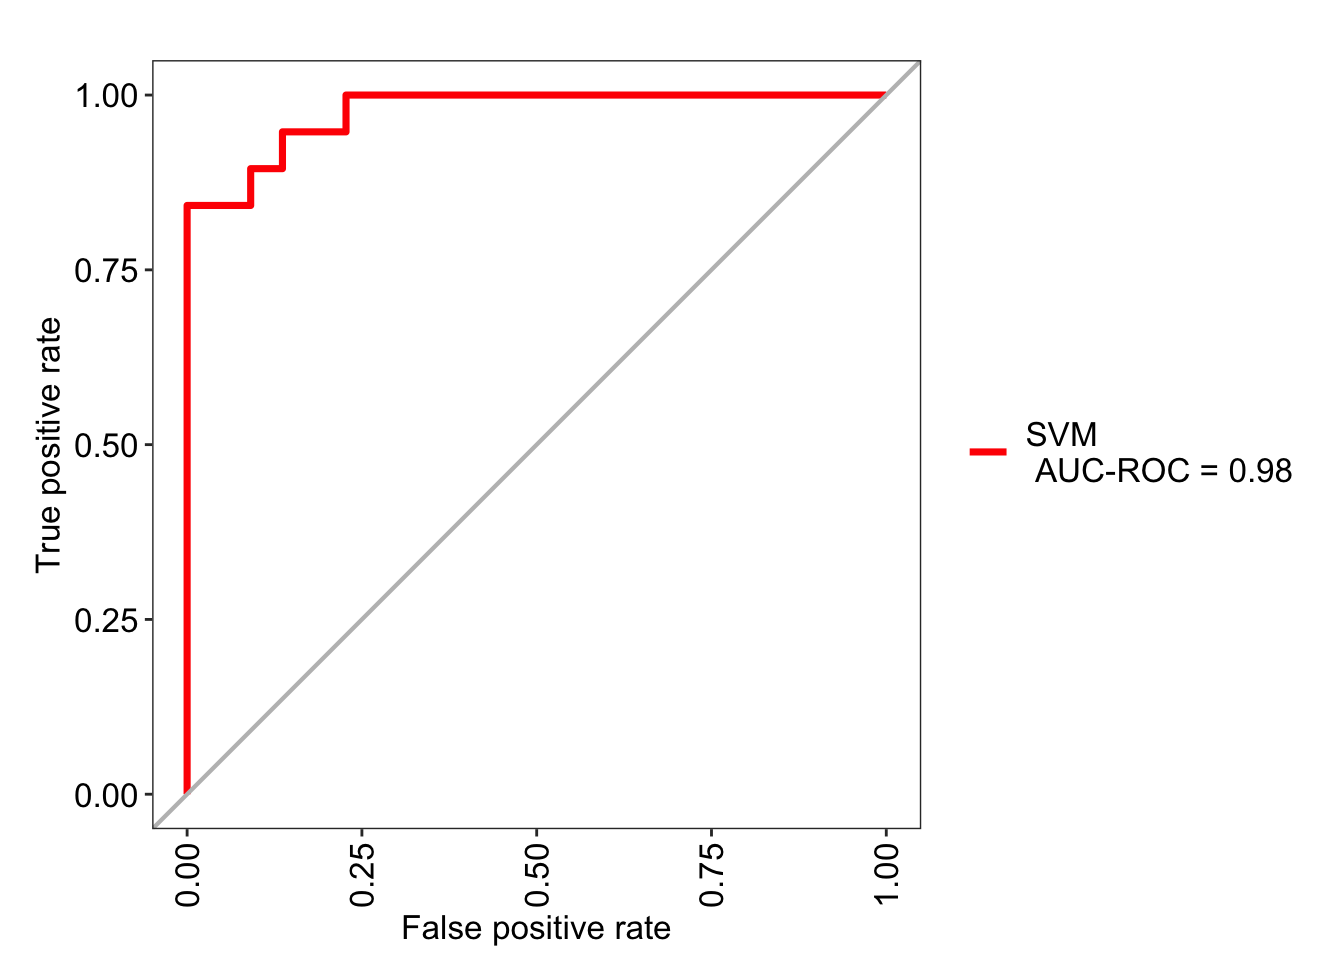
\includegraphics{_main_files/figure-latex/unnamed-chunk-224-1.pdf}

\begin{Shaded}
\begin{Highlighting}[]
\NormalTok{roc\_svm}\SpecialCharTok{$}\NormalTok{proc}
\end{Highlighting}
\end{Shaded}

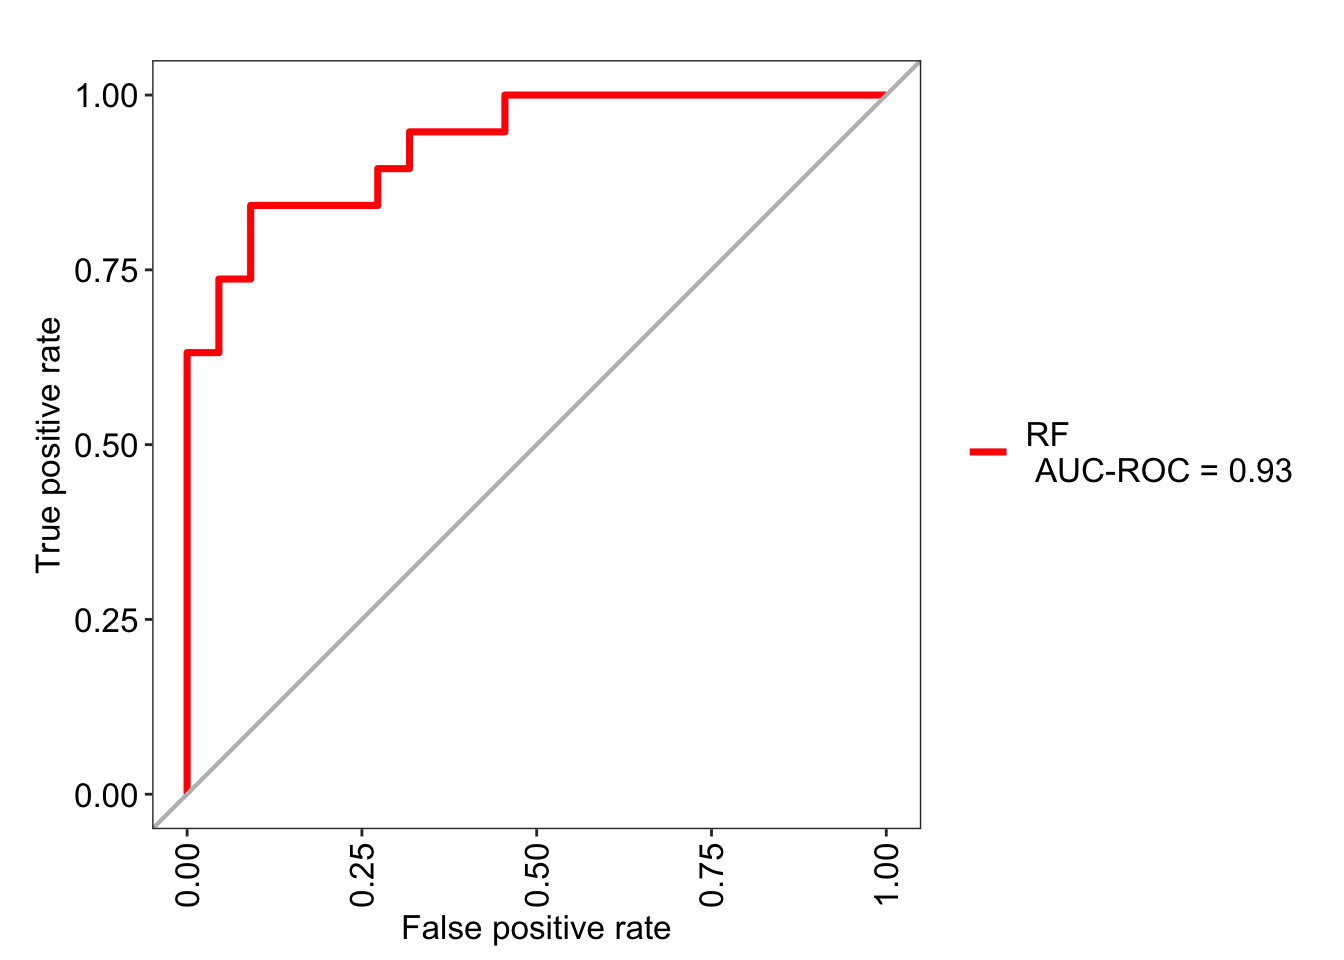
\includegraphics{_main_files/figure-latex/unnamed-chunk-225-1.pdf}

\hypertarget{model-comparisons}{%
\section{Model comparisons}\label{model-comparisons}}

\texttt{caret} provides an elegant way to compare the performance of multiple models for model selection. We have two models trained on \texttt{Sonar} dataset already, so I will train two more.

Here I am using a gradient boosted machine (\texttt{gbm}) and a k-nearest neighbors (\texttt{knn}).

\begin{Shaded}
\begin{Highlighting}[]
\CommentTok{\# model\_rf}
\CommentTok{\# model\_svm}
\NormalTok{model\_gbm }\OtherTok{\textless{}{-}} \FunctionTok{train}\NormalTok{(Class }\SpecialCharTok{\textasciitilde{}}\NormalTok{., }\AttributeTok{data =}\NormalTok{ df\_train, }
                   \AttributeTok{method =} \StringTok{\textquotesingle{}gbm\textquotesingle{}}\NormalTok{, }\AttributeTok{trControl =}\NormalTok{ tr, }
                   \AttributeTok{verbose =} \ConstantTok{FALSE}\NormalTok{)}

\NormalTok{model\_knn }\OtherTok{\textless{}{-}} \FunctionTok{train}\NormalTok{(Class }\SpecialCharTok{\textasciitilde{}}\NormalTok{ ., }\AttributeTok{data =}\NormalTok{ df\_train,}
                   \AttributeTok{method =} \StringTok{\textquotesingle{}knn\textquotesingle{}}\NormalTok{, }\AttributeTok{trControl =}\NormalTok{ tr)}
\end{Highlighting}
\end{Shaded}

\begin{Shaded}
\begin{Highlighting}[]
\NormalTok{model\_gbm}
\end{Highlighting}
\end{Shaded}

\begin{verbatim}
## Stochastic Gradient Boosting 
## 
## 167 samples
##  60 predictor
##   2 classes: 'M', 'R' 
## 
## No pre-processing
## Resampling: Cross-Validated (5 fold) 
## Summary of sample sizes: 134, 133, 134, 133, 134 
## Resampling results across tuning parameters:
## 
##   interaction.depth  n.trees  Accuracy   Kappa    
##   1                   50      0.8263815  0.6476087
##   1                  100      0.8500891  0.6962862
##   1                  150      0.8438503  0.6846292
##   2                   50      0.8074866  0.6102189
##   2                  100      0.8376114  0.6720095
##   2                  150      0.8556150  0.7082185
##   3                   50      0.8379679  0.6717409
##   3                  100      0.8436720  0.6837614
##   3                  150      0.8557932  0.7087382
## 
## Tuning parameter 'shrinkage' was held constant at a value
##  of 0.1
## Tuning parameter 'n.minobsinnode' was held
##  constant at a value of 10
## Accuracy was used to select the optimal model using
##  the largest value.
## The final values used for the model were n.trees =
##  150, interaction.depth = 3, shrinkage = 0.1
##  and n.minobsinnode = 10.
\end{verbatim}

\begin{Shaded}
\begin{Highlighting}[]
\NormalTok{model\_knn}
\end{Highlighting}
\end{Shaded}

\begin{verbatim}
## k-Nearest Neighbors 
## 
## 167 samples
##  60 predictor
##   2 classes: 'M', 'R' 
## 
## No pre-processing
## Resampling: Cross-Validated (5 fold) 
## Summary of sample sizes: 133, 133, 134, 134, 134 
## Resampling results across tuning parameters:
## 
##   k  Accuracy   Kappa    
##   5  0.7852050  0.5633587
##   7  0.7672014  0.5278251
##   9  0.7433155  0.4775343
## 
## Accuracy was used to select the optimal model using
##  the largest value.
## The final value used for the model was k = 5.
\end{verbatim}

Both accuracy and kappa are then used to compare the model performance across the four models:

\begin{Shaded}
\begin{Highlighting}[]
\NormalTok{comps }\OtherTok{\textless{}{-}} \FunctionTok{resamples}\NormalTok{(}
  \FunctionTok{list}\NormalTok{(}\AttributeTok{RF =}\NormalTok{ model\_rf, }\AttributeTok{SVM =}\NormalTok{ model\_svm, }\AttributeTok{GBM =}\NormalTok{ model\_gbm, }
       \AttributeTok{KNN =}\NormalTok{ model\_knn)}
\NormalTok{  )}

\FunctionTok{summary}\NormalTok{(comps)}
\end{Highlighting}
\end{Shaded}

\begin{verbatim}
## 
## Call:
## summary.resamples(object = comps)
## 
## Models: RF, SVM, GBM, KNN 
## Number of resamples: 5 
## 
## Accuracy 
##          Min.   1st Qu.    Median      Mean   3rd Qu.
## RF  0.7941176 0.8235294 0.8484848 0.8450646 0.8529412
## SVM 0.8181818 0.8235294 0.8750000 0.8680481 0.8823529
## GBM 0.7575758 0.8484848 0.8529412 0.8557932 0.8787879
## KNN 0.7058824 0.7272727 0.7352941 0.7852050 0.8484848
##          Max. NA's
## RF  0.9062500    0
## SVM 0.9411765    0
## GBM 0.9411765    0
## KNN 0.9090909    0
## 
## Kappa 
##          Min.   1st Qu.    Median      Mean   3rd Qu.
## RF  0.5853659 0.6382979 0.6857143 0.6844312 0.7017544
## SVM 0.6250000 0.6382979 0.7490196 0.7316302 0.7638889
## GBM 0.5056180 0.6961326 0.7017544 0.7087382 0.7582418
## KNN 0.4055944 0.4469274 0.4593640 0.5633587 0.6892655
##          Max. NA's
## RF  0.8110236    0
## SVM 0.8819444    0
## GBM 0.8819444    0
## KNN 0.8156425    0
\end{verbatim}

And finally, a quick visualization at the model performance comparisons:

\begin{Shaded}
\begin{Highlighting}[]
\FunctionTok{dotplot}\NormalTok{(comps)}
\end{Highlighting}
\end{Shaded}

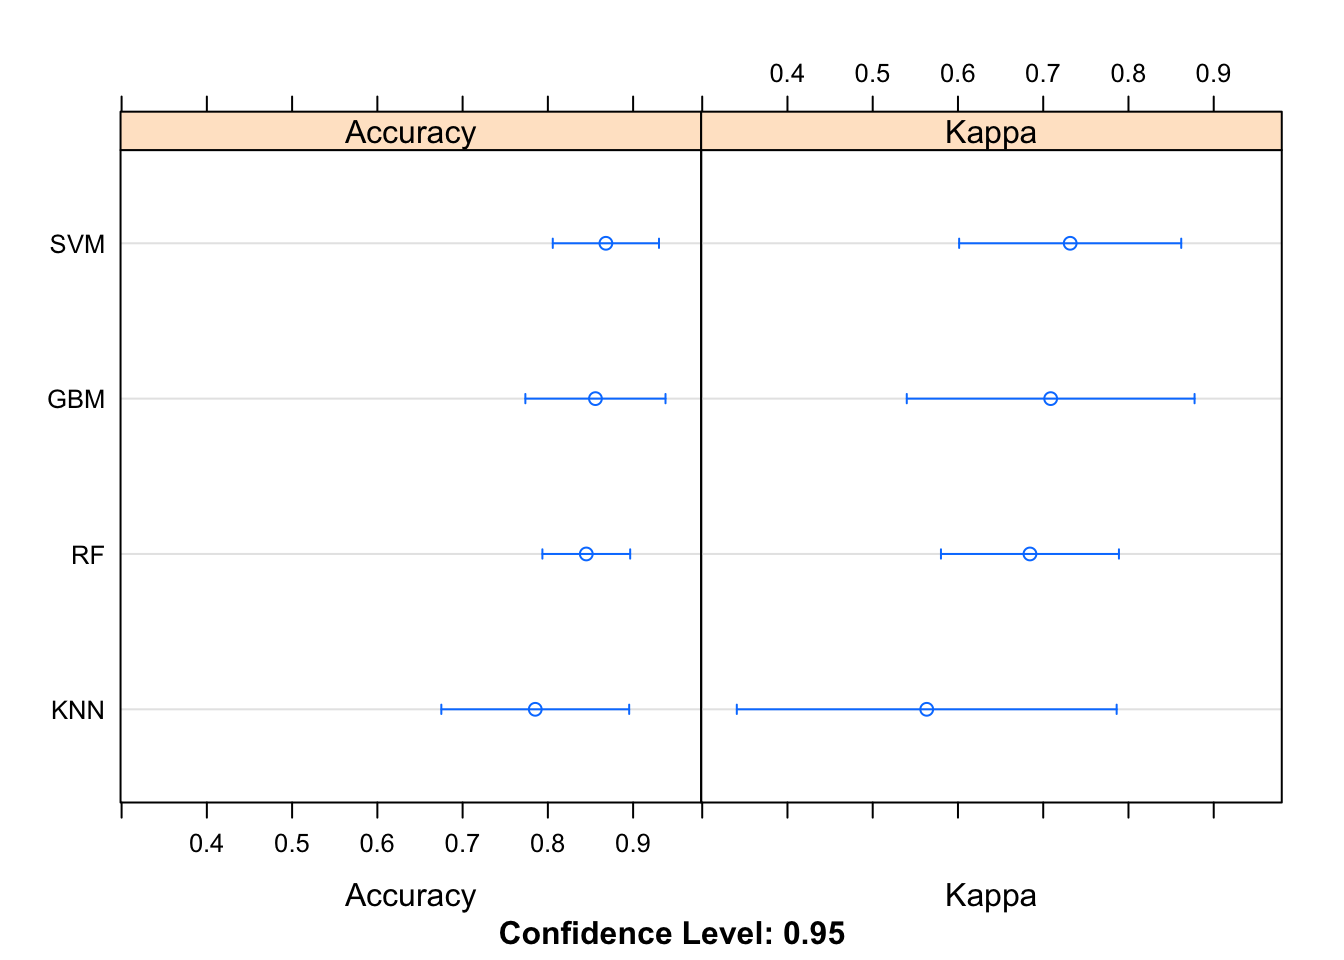
\includegraphics{_main_files/figure-latex/unnamed-chunk-230-1.pdf}

\end{document}
